% $Id: cryptomethods.tex 3712 2016-03-22 23:36:46Z xesslinger $
% !Mode:: "TeX:DE"    % Setting document mode and submode for WinEdt
% ..............................................................................
% B i t b l o c k -  u n d  B i t s t r o m - V e r s c h l ü s s e l u n g
% ~~~~~~~~~~~~~~~~~~~~~~~~~~~~~~~~~~~~~~~~~~~~~~~~~~~~~~~~~~~~~~~~~~~~~~~~~~~~~~

\begin{refsegment}


%BERM0 Changed when bc becoming part of the CT book.
%BERM1 Transformed to comment when bc becoming part of the CT book: There it already was in script-en.tex.
%BERM2 Transformed to comment when bc becoming part of the CT book: Added there to script-en.tex.
%BERM3 Redefined new commands already existing in moderncryptography.tex when bc becoming part of the CT book
%BERM3 (see http://tex.stackexchange.com/questions/36175/what-do-newcommand-renewcommand-and-providecommand-do-and-how-do-they-differ).

%BERM1 \documentclass[11pt,a4paper,leqno]{report}
%BERM1 \usepackage[latin1]{inputenc}
%BERM1 \usepackage[T1]{fontenc}
%BERM1 \usepackage{german}
%BERM1 \usepackage{amsmath,amssymb,amscd,latexsym}
%BERM1 \usepackage{color}
%BERM1 \usepackage{hyperref}
%BERM1 \usepackage{makeidx}
%BERM1 \usepackage[pdftex]{graphicx}
%BERM1 \usepackage{float}

% ++++++++++++++++++++++++++++++++++++++++++++++++++++++++++++++++++++++++++
% Pommerenings Spezialitäten
% ~~~~~~~~~~~~~~~~~~~~~~~~~~~~~~~~~~~~~~~~~~~~~~~~~~~~~~~~~~~~~~~~~~~~~~~~~~

%\newcommand*{\Oh}{\operatorname{O}}

% ++++++++++++++++++++++++++++++++++++++++++++++++++++++++++++++++++++++++++
% CrypTool-Spezialitäten
% ~~~~~~~~~~~~~~~~~~~~~~~~~~~~~~~~~~~~~~~~~~~~~~~~~~~~~~~~~~~~~~~~~~~~~~~~~~
%BERM1 \newtheorem{definition}{Definition}[section]
%BERM1 \newtheorem{satz}{Satz}[section]
%BERM1 \newenvironment{Beweis}[1]{\noindent\textbf{Beweis #1} \\}{\hfill$\Box$\par}
%BERM1 \newenvironment{example}[1]{\noindent\textbf{Beispiel#1}}{}
%BERM1 \newenvironment{remark}[1]{\noindent\textbf{Bemerkung#1}}{}
%BERM1 \setcounter{secnumdepth}{4} % Nummerierung auch bei subsubsection
%BERM1 \floatstyle{ruled}
%BERM1 \newfloat{sagecode}{!ht}{loc}[chapter]
%BERM1 \floatname{sagecode}{SageMath-Beispiel}

\sloppy
\frenchspacing
%BERM1 \makeindex
%BERM1 \begin{document}

%BERM0 \setcounter{chapter}{98}  % ====> Dummy - beim Einfügen ins CT-Skript löschen <=====
\setcounter{satz}{0}
\setcounter{definition}{0}


\newpage %BERM0
\hypertarget{Chapter_BitCiphers}{}   %BERM0
\chapter{Einführung in die Bitblock- und Bitstrom-Verschlüsselung}
\chaptermark{Einführung Bit-Verschlüsselung}
\label{Chapter_BitCiphers}
(\hyperlink{author_Klaus-Pommerening}{Klaus Pommerening},
 Januar--Juni 2015; Updates: Jan. 2016, Apr. 2016) \\

\noindent
Während asymmetrische Verschlüsselung meistens zahlentheoretische Methoden
verwendet, beruhen die heutigen symmetrischen
Verschlüsselungsverfahren\index{Verschlüsselung!symmetrisch}
in der Regel auf Boolescher Algebra\index{Boolesche Algebra}\index{Algebra!Boolesche},
d.\,h., auf Manipulationen von Bits.
Das ist eine ganz andere Art von Mathematik, für Einsteiger vielleicht
ungewohnt, so dass dieses Kapitel eine sanfte Einführung in dieses mathematische
Gebiet sein soll. Vorkenntnisse aus einem Grundkurs Mathematik am Gymnasium
sollen ausreichen. Ohne weitere Erklärung als bekannt
angenommen werden die Begriffe "`Variable"' und "`Funktion"', auch für Argumente
und Werte in anderen Mengen als den reellen Zahlen.

Beginnen wir also mit der Beschreibung, wie Bits interpretiert, verknüpft
und durch Funktionen, sogenannte Boolesche
Funktionen\index{Boolesche Funktion}\index{Funktion!Boolesche}, verarbeitet werden.
Namenspatron dieses Fachgebiets ist
George Boole\index{Boole, George}\footnote{%
  George Boole, englischer Mathematiker, Logiker und Philosoph,
  2.11.1815--8.12.1864.
},
der durch die Einführung der elementaren logischen Operationen die Logik
mathematisch formalisierte ("`Logikkalkül\index{Logikkalkül}"').
Moderne symmetrische Verschlüsselungsverfahren, wie auch
Hash-Funktionen\index{Hashfunktion},
werden durch Systeme von Booleschen Funktionen beschrieben.

Der Schwerpunkt dieses Kapitels liegt in der Einführung in die
mathematischen Grundlagen der Verschlüsselungstechniken, die auf
Bits operieren. Konkrete Verfahren werden nicht detailliert beschrieben;
hierfür sei auf die Bücher von
Menezes/Orschot/Vanstone \cite{Menezes2001},
Oppliger \cite{Oppliger2011},
Paar und Pelzl \cite{PaPe2009},
Schmeh \cite{Schm2003, Schm2016}
und Stamp \cite{Stamp2007} verwiesen.

Noch ein Wort zur Nomenklatur: Die Verfahren werden in der Literatur
meist als "`Blockchiffren\index{Blockchiffre}"' oder
"`Stromchiffren\index{Stromchiffre}"' bezeichnet, ohne
das Präfix "`Bit-"'. Das ist manchmal missverständlich, da -- besonders
bei Stromchiffren -- auch andere Zeichensätze (Alphabete, Buchstaben)
als kleinste Einheiten verwendet werden. Der Deutlichkeit halber
sollte man im Zweifelsfall also die "`Bits"' mit in die Bezeichnung
aufnehmen.

Das Thema dieses Kapitels ist also mit anderen Worten

%\begin{quote}
   {\bf Symmetrische Verschlüsselung von mit Bits dargestellten Informationen}.
%\end{quote}

\noindent Die mathematischen Grundlagen und Methoden gehören zu den Gebieten

   {\bf Boolesche Algebra\index{Boolesche Algebra}\index{Algebra!Boolesche}
   und endliche Körper\index{endlicher Körper}\index{Körper!endlich}}.


% ++++++++++++++++++++++++++++++++++++++++++++++++++++++++++++++++++++++++++
\newpage
\section{Boolesche Funktionen}\label{s-bool-fct}
\subsection{Bits und ihre Verknüpfung}\label{s-bool-bit}

Die Objekte, mit denen Computer auf der untersten Software-Ebene operieren,
sind Bits\index{Bit} oder Gruppen von Bits (z.\,B. Bytes\index{Byte},
die meist aus 8 Bits bestehen,
oder "`Wörter\index{Wort}"', je nach Computer-Architektur meist 32 oder 64 Bits).
Der Umgang mit den Bits $0$ und $1$ und mit den elementaren
logischen Operationen wie "`und"' (AND), "`oder"' (OR),
"`nicht"' (NOT) und "`exklusives oder"' (XOR) ist zwar den meisten
vertraut, soll aber hier kurz beschrieben werden, auch um die verwendete
Terminologie einzuführen.

Bits können logisch interpretiert werden als die
Wahrheitswerte\index{Wahrheitswert} "`wahr"'
(True, T) und "`falsch"' (False, F). Sie können auch algebraisch interpretiert
werden als die Werte $0$ (entspricht F) und $1$ (entspricht T). Mathematisch
gesprochen sind sie dann Elemente der zweielementigen Menge $\{0, 1\}$,
die wir hinfort in diesem Kapitel mit $\F_2$ bezeichnen werden; warum,
wird gleich erklärt:

Betrachtet man nämlich den Restklassenring von $\Z$ modulo $2$, so
hat dieser zwei Elemente und ist ein Körper\index{Körper},
da $2$ eine Primzahl ist. Die Addition in diesem Körper
entspricht genau der logischen Verknüpfung XOR\index{XOR},
die Multiplikation der logischen Verknüpfung AND\index{AND},
wie man in Tabelle~\ref{t-bool-xor} sieht. Tabelle~\ref{t-bool-trf}
listet die Umrechnungsformeln zwischen den elementaren logischen
und algebraischen Operationen auf.

\begin{table}[h]
\begin{center}
\begin{tabular}{|cc|ccc||cc|cc|} \hline
   \multicolumn{5}{|c||}{\bf logisch} & \multicolumn{4}{c|}{\bf algebraisch} \\ \hline
   \multicolumn{2}{|c|}{Bits} & \multicolumn{3}{|c||}{Verknüpfung} &
        \multicolumn{2}{|c|}{Bits} & \multicolumn{2}{|c|}{Verknüpfung} \\ \hline
   $x$ & $y$ & OR & AND & XOR & $x$ & $y$ & + & $\cdot$ \\ \hline
    F  &  F  & F  &  F  &  F  &  0  &  0  &  0  &  0    \\
    F  &  T  & T  &  F  &  T  &  0  &  1  &  1  &  0    \\
    T  &  F  & T  &  F  &  T  &  1  &  0  &  1  &  0    \\
    T  &  T  & T  &  T  &  F  &  1  &  1  &  0  &  1    \\
   \hline
\end{tabular}
\end{center}
\caption{Die wichtigsten Verknüpfungen von Bits\index{Bit}. Dabei ist das logische
  XOR\index{XOR} identisch mit dem algebraischen +, das logische AND\index{AND} mit dem
  algebraischen $\cdot$ (Multiplikation).}\label{t-bool-xor}
\end{table}

\begin{table}[h]
\begin{center}
\begin{tabular}{|rcl|} \hline
   \multicolumn{3}{|c|}{\bf algebraisch nach logisch}          \\ \hline
   $x + y$      & = & $(x \vee y) \wedge (\neg x \vee \neg y)$ \\
   $x \cdot y$  & = & $x \wedge y$                             \\ \hline \hline
   \multicolumn{3}{|c|}{\bf logisch nach algebraisch}          \\ \hline
   $x \vee y$   & = & $x + y + x\cdot y$                       \\
   $x \wedge y$ & = & $x \cdot y$                              \\
   $\neg x$     & = & $1 + x$                                  \\ \hline
\end{tabular}
\end{center}
\caption{Umrechnung der algebraischen Operationen in logische und umgekehrt}\label{t-bool-trf}
\end{table}

Da die algebraische Struktur als Körper\index{Körper} für die Kryptographie
eine herausragende Rolle spielt, wird hier die in der Algebra übliche
Bezeichnung für endliche Körper\index{Körper!endlich} $\F_q$ (oft
auch $\text{GF}(q)$ für "`Galois\index{Galois, Évariste}\footnote{%
  Évariste Galois, französischer Mathematiker,
  25.10.1811--31.5.1832.
}
Field"', dabei ist $q$ die Anzahl der Elemente) übernommen\footnote{%
  Auch SageMath verwendet die Bezeichnung $\text{GF}(q)$.
}.
In diesem Kontext ist es sinnvoll, für die
Verknüpfungen die algebraischen Symbole $+$ (für XOR) und
$\cdot$ (für AND) zu verwenden, wobei der Multiplikationspunkt wie
auch sonst in der Mathematik oft weggelassen wird. Kryptographen benutzen
gerne auch die Symbole $\oplus$ und $\otimes$, die allerdings in der
Mathematik mit ganz anderen Bedeutungen\footnote{%
  direkte Summe und Tensorprodukt von Vektorräumen
}
belegt sind und daher in diesem Text -- abgesehen von Diagrammen --
meist vermieden werden.

Zur Verdeutlichung sei noch explizit auf einige Besonderheiten des
algebraischen Rechnens im binären Fall (d.\,h., in Charakteristik $2$)
hingewiesen:
\begin{itemize}
   \item In einer Summe heben sich zwei gleiche Summanden gegenseitig
      weg, d.\,h., sie ergeben zusammen $0$. Allgemeine Regel: $x + x = 0$
      oder $2x = 0$.
   \item Allgemeiner ergibt eine gerade Anzahl gleicher Summanden immer $0$,
      während eine ungerade Anzahl gleicher Summanden genau diesen Summanden
      ergibt. Allgemeine Regel:
\[
         m \, x := \underbrace{x + \cdots + x}_m \quad = \quad
            \begin{cases}
               0 & \text{für gerades } m \\ x & \text{für ungerades } m.
            \end{cases}
\]
   \item Bei algebraischen Umformungen ist eine Subtraktion dasselbe wie
      eine Addition; man kann Plus- und Minuszeichen beliebig gegeneinander
      austauschen. Allgemeine Regel: $x + y = x - y$.
   \item Alle drei binomischen Formeln, also für $(x + y)^2$, $(x - y)^2$,
      $(x + y)(x - y)$, fallen zu einer einzigen zusammen:
\[
         (x + y)^2 = x^2 + y^2.
\]
      Denn das doppelte Produkt ist $0$.
\end{itemize}


\subsection{Beschreibung Boolescher Funktionen}\label{ss-bool-descr}

Definieren wir zunächst ganz naiv: Eine {\bf Boolesche
Funktion}\index{Boolesche Funktion}\index{Funktion!Boolesche} ist eine
Vorschrift (oder eine Rechenregel oder ein Algorithmus), die aus einer
bestimmten Anzahl von Bits ein neues Bit erzeugt. Bevor wir diese
Definition mathematisch präzise fassen (siehe Definition~\ref{def-bool-fkt}),
soll sie zunächst etwas anschaulicher gemacht werden.

Für eine vertiefte Darstellung sei auf \cite{CuSt2009} oder \cite{Pomm2008, Pomm2014}
sowie die beiden Artikel von Claude Carlet\footnote{%
  siehe auch dessen Publikationsverzeichnis unter
  %BERM \url statt \href
  % \href{http://www.math.univ-paris13.fr/~carlet/pubs.html}{\tt http://www.math.univ-paris13.fr/$\sim$carlet/pubs.html}
  \url{http://www.math.univ-paris13.fr/~carlet/pubs.html}
} in \cite{CrHa2010}\footnote{%
  online zu finden unter
  \url{http://www.math.univ-paris13.fr/~carlet/chap-fcts-Bool-corr.pdf}  und
  \url{http://www.math.univ-paris13.fr/~carlet/chap-vectorial-fcts-corr.pdf}
} verwiesen.

Als ganz einfaches Musterbeispiel dient die Funktion AND\index{AND}: Sie nimmt zwei Bits
entgegen und erzeugt daraus ein neues Bit nach der bekannten Verknüpfungsregel
des logischen "`und"', siehe Tabelle~\ref{t-bool-xor}.

Als etwas komplizierteres Beispiel möge die Funktion $f_0$ dienen, die aus drei Bits
$x_1$, $x_2$ und $x_3$ den Wert
\begin{equation}\label{bc_sample-fct-f0-with-3-vars}
   f_0(x_1, x_2, x_3) = x_1\: \text{AND}\: (x_2\: \text{OR}\: x_3)
\end{equation}
% Hier equation statt  \[...\]  oder  $$...$$, die wohl äqivalent sind. Vorher war:
%  \[
%     f_0(x_1, x_2, x_3) = x_1\: \text{AND}\: (x_2\: \text{OR}\: x_3)
%  \]
berechnet.

Veranschaulichen kann man sich eine Boolesche Funktion durch eine
"`Black Box\index{Black Box}"':
\begin{center}
\begin{picture}(140,60)
   \put(20,25){\colorbox{black}{XgXXXXXXXXXX}}
%   \put(20,20){\framebox(100,20){$f$}}
   \put(25,35){\line(0,1){10}}
   \put(35,35){\line(0,1){10}}
   \put(45,35){\line(0,1){10}}
   \put(65,40){\ldots}
   \put(95,35){\line(0,1){10}}
   \put(105,35){\line(0,1){10}}
   \put(115,35){\line(0,1){10}}
   \put(70,20){\line(0,-1){10}}
   \put(48,50){\sf Input-Bits}
   \put(48,0){\sf Output-Bit}
\end{picture}
\end{center}

\noindent Was innerhalb dieser "`Black Box"' passiert, kann man auf verschiedene
Arten beschreiben:
\begin{itemize}
   \item {\bf mathematisch} durch eine Formel,
   \item {\bf informatisch} durch einen Algorithmus,
   \item {\bf technisch} durch ein Schaltnetz\index{Schaltnetz}
      (oder Schaltdiagramm),
   \item {\bf pragmatisch} durch eine Wahrheitstafel\index{Wahrheitstafel}
      (das ist die Wertetabelle).
\end{itemize}
Die Beispielfunktion $f_0$ ist mathematisch definiert in der
Gleichung~(\ref{bc_sample-fct-f0-with-3-vars}). Der entsprechende Algorithmus
wird hier am besten ebenfalls durch diese Formel beschrieben, da keinerlei
Verzweigungen oder bedingte Anweisungen nötig sind. Als Schaltnetz kann man
$f_0$ etwa wie in Abbildung~\ref{fig-bool-circuit} visualisieren.
Die Wahrheitstafel gibt zu jedem Input-Tripel einfach den Wert von $f_0$ an,
siehe Tabelle~\ref{tab-bool-wt}.

\begin{figure}[h]
\begin{center}
\begin{picture}(130,90)
   \put(58,30){AND}
   \put(70,29){\vector(0,-1){20}}
   \put(45,0){$f_0(x_1,x_2,x_3)$}
   \put(22,80){$x_1$}
   \put(67,80){$x_2$}
   \put(109,80){$x_3$}
   \put(88,55){OR}
   \put(90,51){\vector(-1,-1){10}}
   \put(110,75){\vector(-1,-1){10}}
   \put(78,75){\vector(1,-1){10}}
   \put(30,75){\vector(1,-1){34}}
\end{picture}
\end{center}
\caption{Beispiel eines Schaltnetzes}\label{fig-bool-circuit}
\end{figure}

\begin{table}[hbpt]
\begin{center}
\begin{tabular}{|ccc|c|} \hline
   $x_1$ & $x_2$ & $x_3$ & $f_0(x_1,x_2,x_3)$ \\ \hline
      0  &   0   &   0   &  0  \\
      0  &   0   &   1   &  0  \\
      0  &   1   &   0   &  0  \\
      0  &   1   &   1   &  0  \\
      1  &   0   &   0   &  0  \\
      1  &   0   &   1   &  1  \\
      1  &   1   &   0   &  1  \\
      1  &   1   &   1   &  1  \\
   \hline
\end{tabular}
\end{center}
\caption{Beispiel einer Wahrheitstafel}\label{tab-bool-wt}
\end{table}

Die Bezeichnung "`Wahrheitstafel\index{Wahrheitstafel}"' kommt von der Interpretation der
Bits im Logikkalkül\index{Logikkalkül}: 0 (= F) bedeutet "`falsch"', 1 (= T) bedeutet "`wahr"'.
Der Wert $f(x_1,\ldots,x_n)$ einer Booleschen Funktion $f$ sagt dann,
ob der gesamte Ausdruck wahr oder falsch ist, wenn die einzelnen Input-Bits
$x_1,\ldots,x_n$ die angegebenen Wahrheitswerte haben.

Die Verbindung zur Technik, also die Beziehung zwischen Logikkalkül
und elektrischen Schaltungen, wurde im Wesentlichen von
Shannon\index{Shannon, Claude}\footnote{%
  Claude Elwood Shannon, amerikanischer Mathematiker und Elektrotechniker,
  30.4.1916--24.2.2001.
}
entwickelt.

\subsection{Die Anzahl Boolescher Funktionen}\label{ss-bool-enum}

Die obige Wahrheitstafel für $f_0$ suggeriert eine einfache Abzählung aller
Booleschen Funktionen:
Bei drei Variablen gibt es $8 = 2^3$ verschiedene Input-Tripel, denn jedes
einzelne Input-Bit kann unabhängig von den beiden anderen Bits die Werte $0$ oder $1$
annehmen. Eine Boolesche Funktion $f$ wiederum kann für jedes Input-Tripel
unabhängig von den sieben anderen Tripeln $0$ oder $1$ werden, das
sind $8$ unabhängige Möglichkeiten für $0$ oder $1$, also insgesamt $2^8$.
Also gibt es $256 = 2^8$ Boolesche Funktionen von drei Variablen.

Im allgemeinen Fall haben wir $N = 2^n$ verschiedene Besetzungen für
die $n$ Input-Variablen, und für jeden dieser $N$ Inputs kann die
Funktion $0$ oder $1$ werden, das macht $2^N$ verschiedene
Möglichkeiten. Die allgemeine Formel ist also:

\begin{satz}\label{thm-bool-enum}
   Es gibt genau $2^{2^n}$ verschiedene Boolesche Funktionen von
   $n$ Variablen.
\end{satz}

Bei vier Variablen sind das schon $2^{16} = 65536$ Stück, und die Formel
sagt, dass die Anzahl superexponenziell\index{superexponenziell} anwächst: Der Exponent wächst
ja selbst schon exponenziell.

Alle 16 Booleschen Funktionen von zwei Variablen sind im
Abschnitt~\ref{ss-bool-2}, Tabelle~\ref{tab-bool-2}, aufgelistet.

\subsection{Bitblöcke und Boolesche Funktionen}\label{ss-bool-blck}

Für Gruppierungen von Bits gibt es je nach Kontext verschiedene
Bezeichnungen\footnote{%
   Begrifflich beschreiben sie das gleiche. In Python\index{Python} bzw. SageMath
   entsprechen den verschiedenen Bezeichnungen aber z.\,T. unterschiedliche
   Typen.
}:
Vektoren\index{Vektor}, Listen\index{Liste}, ($n$-) Tupel\index{Tupel},
\ldots, bei bestimmten Größen auch spezielle Bezeichnungen wie Bytes\index{Byte}
(für 8 Bits), Wörter\index{Wort} (für 32 oder
64 Bytes, je nach Prozessorarchitektur) \ldots\
In diesem Kapitel wird überwiegend
die in der Kryptographie gängige Bezeichnung "`Bitblöcke\index{Bitblock}"' verwendet.
Ein {\bf Bitblock} der Länge $n$ ist also eine Liste $(x_1, \ldots, x_n)$ von
Bits. Hierbei kommt es auf die Reihenfolge an. Es gibt acht
verschiedene Bitblöcke der Länge $3$. Dies sind sie:
\[
   (0,0,0), (0,0,1), (0,1,0), (0,1,1), (1,0,0), (1,0,1), (1,1,0), (1,1,1).
\]
Gelegentlich werden sie, wenn dadurch kein Missverständnis zu befürchten ist, auch
ohne Klammern und Kommas als Bitketten\index{Bitkette} geschrieben\footnote{%
   Manchmal werden sie auch in Spaltenform, als $n \times 1$-Matrizen,
   geschrieben, wenn die Interpretation als Vektor\index{Vektor} im Vordergrund steht.
}:
\[
   000, 001, 010, 011, 100, 101, 110, 111.
\]

Oft wird die abgekürzte Schreibweise $x$ für $(x_1, \ldots, x_n)$ verwendet,
die ausdrückt, dass
Bitblöcke\index{Bitblock} Objekte "`eigenen Rechts"' sind. Die $2^n$ verschiedenen
Bitblöcke der Länge $n$ sind genau die Elemente des kartesischen Produkts
$\F_2^n = \F_2 \times \cdots \times \F_2$. Dieses kartesische Produkt
hat eine "`natürliche"' Vektorraum-Struktur\index{Vektorraum} -- man kann Bitblöcke
$x$ und $y \in \F_2^n$ addieren und mit Skalaren $a \in \F_2$ multiplizieren:
\[
   (x_1, \ldots, x_n) + (y_1, \ldots, y_n) =  (x_1 + y_1, \ldots, x_n + y_n),
\]
\[
   a \cdot (x_1, \ldots, x_n) = (a \cdot x_1, \ldots, a \cdot x_n).
\]

Damit können wir nun die mathematisch exakte Definition formulieren:

\begin{definition}\label{def-bool-fkt}\index{Boolesche Funktion}\index{Funktion!Boolesche}
  Eine {\bf Boolesche Funktion von $n$ Variablen} ist eine Abbildung
\[
     f\!\!: \F_2^n \longrightarrow \F_2.
\]
\end{definition}
Eine solche nimmt als Argument also einen Bitblock\index{Bitblock} der Länge $n$
und produziert daraus ein Bit.

Die Menge aller Booleschen Funktionen auf $\F_2^n$ wird im Folgenden gelegentlich
mit $\mathcal{F}_n$ bezeichnet. Nach Satz~\ref{thm-bool-enum} hat sie
$2^{2^n}$ Elemente.

\begin{description}
   \item[Konvention:] Beschreibt man eine Boolesche Funktion durch ihre
      Wahrheitstafel, so ordnet man diese, wie auch oben im Beispiel
      schon gesehen, in der Regel lexikographisch\index{lexikographisch}\footnote{%
        Bei einer lexikographischen Ordnung\index{Ordnung!lexikographisch}
        werden die zu ordnenden
        Zeichenketten (wie in einem Lexikon) nach der Größe des ersten
        Zeichens -- hier $0$ oder $1$ mit $0 < 1$ -- geordnet.
        Falls dieses gleich ist, nach der Ordnung des zweiten Zeichens
        usw. Lexikographisch geordnet ist die Folge $011,100,101$. Nicht
        lexikographisch geordnet die Folge $100,101,011$, weil hier die
        dritte Zeichenkette mit einer $0$ beginnt, die kleiner ist als das
        Anfangszeichen der davor stehenden Zeichenkette. Die zu Beginn
        von \ref{ss-bool-blck} aufgeschriebene Reihenfolge der acht
        Bitblöcke der Länge $3$ folgt der lexikographischen Ordnung.
      } nach $x \in \F_2^n$;
      diese Ordnung ist, anders ausgedrückt, die natürliche Ordnung der
      Zahlen $a = 0, \ldots, 2^n-1$, wenn diese binär als
\[
     a = x_1\cdot 2^{n-1} + \cdots + x_{n-1}\cdot 2 + x_n
\]
      dargestellt und auf diese Weise den Bitblöcken\index{Bitblock}
      $(x_1,\ldots,x_n) \in \F_2^n$ zugeordnet werden.
\end{description}

\subsection{Logische Ausdrücke und disjunktive Normalform}\label{ss-bool-dnf}

Für die mathematische Beschreibung Boolescher Funktionen, also wie
oben gesagt die Beschreibung durch eine Formel, sind im wesentlichen
außer der Wahrheitstafel zwei Ansätze gebräuchlich:
\begin{itemize}
   \item In der Logik werden Boolesche Funktionen durch Disjunktionen\index{Disjunktion}
      (die Operation OR\index{OR}, auch $\vee$ geschrieben), Konjunktionen\index{Konjunktion}
      (die Operation AND\index{AND}, auch $\wedge$ geschrieben) und Negationen
      (die Operation NOT\index{NOT}, auch $\neg$ geschrieben) ausgedrückt.
      Zusammensetzungen dieser Operationen heißen {\bf logische
      Ausdrücke}\index{logischer Ausdruck}\index{Ausdruck!logisch}.
   \item In der Algebra werden Boolesche Funktionen durch die
      Addition $+$ und die Multiplikation $\cdot$ des Körpers $\F_2$
      ausgedrückt. Zusammensetzungen dieser Operationen heißen
      {\bf (binäre) polynomiale
      Ausdrücke\index{polynomialer Ausdruck}\index{Ausdruck!polynomial}}\footnote{%
        Nicht polynomial wären Ausdrücke, in denen andere Verknüpfungen
        vorkommen. Bei Zahlen könnte man hier auch daran denken,
        Inputvariablen als Exponenten zu verwenden, das ergibt bei den
        Booleschen Variablen $0$ und $1$ allerdings keinen rechten Sinn.
      }.
\end{itemize}
Wir werden bald sehen, dass man auf beide Weisen alle Booleschen
Funktionen\index{Boolesche Funktion}\index{Funktion!Boolesche}
beschreiben kann und dass dabei sogar zusätzliche Anforderungen
an die Gestalt der Formeln, sogenannte Normalformen, gestellt werden
können. Selbstverständlich kann man auch für jede Boolesche Funktion
zwischen den drei Darstellungsarten Wahrheitstafel, logischer Ausdruck
und binärer polynomialer Ausdruck hin- und herwechseln. Dass die
Algorithmen dafür bei großer Zahl $n$ von Variablen effizient sind,
ist aber nicht zu erwarten, denn schon allein das Aufschreiben einer
Wahrheitstafel\index{Wahrheitstafel} erfordert $2^n$ Bits. Für die algorithmische Behandlung
Boolescher Funktionen in SageMath siehe auch Anhang~\ref{a-bool-sage}.

Die algebraische Form scheint für kryptologische Zwecke aufgrund ihrer
(noch zu erkundenden)
Strukturiertheit etwas besser zu handhaben sein. Die logische Form führt
dagegen einfacher zu einer Hardware-Realisierung durch ein Schaltnetz\index{Schaltnetz},
weil die elementaren Booleschen Operationen direkte Entsprechungen
in Schaltelementen ("`Gatter\index{Gatter}"') haben.

Da die logische Form im Folgenden eine geringere Rolle spielt, wird
das Ergebnis hier ohne weitere Begründung angegeben; die bloße Möglichkeit
der Darstellung durch die logischen Operationen (ohne Normalisierung)
folgt im Abschnitt~\ref{ss-bool-2} noch einmal als Nebenergebnis,
siehe Satz~\ref{thm-bool-log}.

\begin{satz}\label{thm-bool-disj}
   Jede Boolesche Funktion von $n$ Variablen $x_1, \ldots, x_n$ lässt
   sich mit einem geeigneten $r$ in der Form (Konjunktion\index{Konjunktion})
\[
     f(x) = s_1(x) \wedge \ldots \wedge s_r(x)
\]
   schreiben, wobei die $s_j(x)$ für $j = 1, \ldots, r$ jeweils die
   Gestalt (Disjunktionen\index{Disjunktion})
\[
     s_j(x) = t_{j1}(x) \vee \ldots \vee t_{jn_j}(x)
\]
   mit einer Anzahl $n_j$ von Termen $t_{jk}(x)$ ($j = 1, \ldots, r$
   und $k = 1, \ldots, n_j$) haben, die selbst jeweils
   von der Gestalt $x_i$ (Input-Bit) oder
   $\neg x_i$ (negiertes Input-Bit) für jeweils einen Index $i$
   sind\footnote{%
   Insbesondere ist $n_j \leq n$ für $j = 1, \ldots,r$.
   Ein einzelnes Input-Bit $x_i$ kommt in jedem der $t_{jk}(x)$
   entweder direkt oder negiert oder gar nicht vor.}.
\end{satz}
Mit anderen Worten: Man kann jede Boolesche
Funktion\index{Boolesche Funktion}\index{Funktion!Boolesche} aufbauen, indem
man einige Ausdrücke (die $s_j(x)$) durch OR\index{OR}-Verknüpfung von einigen der
Input-Bits oder deren Negation bildet, und diese Ausdrücke dann
mit AND\index{AND} verbindet ("`Konjunktion von Disjunktionen"'). Die AND- und
OR-Verknüpfungen sind in dieser "`Normalform"' also sauber
in zwei Schichten getrennt, eine weitere Vermischung kommt nicht vor.
Die Beispielfunktion $f_0$ aus Abschnitt~\ref{ss-bool-descr} hat
die Definitionsgleichung
\[
     f_0(x_1,x_2,x_3)
     = \underbrace{x_1}_{s_1(x)}
     \wedge \underbrace{(x_2 \vee x_3)}_{s_2(x)}.
\]
Diese hat schon die gewünschte "`konjunktive"' Form aus
Satz~\ref{thm-bool-disj} mit
\[
     n_1 = 1, \:\: s_1(x) = t_{11}(x) = x_1, \quad
     n_2 = 2, \:\: t_{21}(x) = x_2, \:\: t_{22}(x) = x_3.
\]
Das gilt nicht mehr, wenn man sie in expandiert:
\[
     f_0(x) = (x_1 \wedge x_2) \vee (x_1 \wedge x_3).
\]
Negierte Input-Bits kommen in diesem Beispiel nicht vor. Solche sieht
man aber in Tabelle~\ref{tab-bool-2} recht häufig.

Die Gestalt einer Booleschen Funktion nach Satz~\ref{thm-bool-disj}
heißt {\bf konjunktive Normalform\index{konjunktive Normalform}\index{Normalform!konjunktiv}
(CNF\index{CNF})}. Sie ist nicht eindeutig\footnote{%
  Z.\,B. könnte man der Normalform von $f_0$ noch die Terme
  $\wedge\: (x_1 \vee x_2) \wedge (x_1 \vee x_3)$ hinzufügen.
}$^,$\footnote{%
  Die Umwandlung eines logischen Ausdrucks in die CNF wird von der Funktion
  {\tt convert\_cnf()} in der mitgelieferten SageMath-Klasse
  {\tt sage.logic.boolformula.BooleanFormula} geleistet, die
  Bestimmung der zugehörigen Wahrheitstafel durch die Funktion
  {\tt truthtable()} dieser Klasse.
}.
Ohne weitere Erklärung sei vermerkt, dass man sie weiter zu einer "`kanonischen
CNF"' vereinfachen kann und damit eine gewisse Eindeutigkeit erhält.
Auch eine analoge disjunktive Normalform\index{disjunktive Normalform}\index{Normalform!disjunktiv}
({\bf DNF\index{DNF}}) ist möglich ("`Disjunktion von Konjunktionen"').

\subsection{Polynomiale Ausdrücke und algebraische Normalform}\label{ss-bool-anf}

Betrachten wir (binäre) polynomiale\index{polynomialer Ausdruck}\index{Ausdruck!polynomial}
Ausdrücke in den Variablen $x_1, \ldots, x_n$,
wie etwa $x_1^2 x_2 + x_2 x_3 + x_3^2$, so verwenden wir als Koeffizienten,
da wir im Körper $\F_2$ rechnen, nur die Konstanten $0$ und $1$, und diese
brauchen in einem solchen Ausdruck gar nicht explizit hingeschrieben zu werden.
Eine weitere Vereinfachung beruht auf der Beobachtung, dass $a^2 = a$ für alle
Elemente $a \in \F_2$ (denn $0^2 = 0$ und $1^2 = 1$). Daher gilt sogar stets
$a^e = a$ für alle Exponenten $e \geq 1$. Für binäre polynomiale Ausdrücke
bedeutet das, dass wir die Variablen $x_1, \ldots, x_n$ nur höchstens in
der ersten Potenz zu berücksichtigen brauchen. Den Beispielausdruck können
wir also auch als $x_1 x_2 + x_2 x_3 + x_3$ schreiben.
Ein anderes Beispiel: $x_1^3 x_2 + x_1 x_2^2 = x_1 x_2 + x_1 x_2 = 0$.

Allgemein hat ein {\bf monomialer Ausdruck\index{monomialer Ausdruck}\index{Ausdruck!monomial}}
(oder einfach nur "`Monom\index{Monom}"') die Gestalt
\[
    x^I := \prod_{i \in I} x_i
     \quad\text{mit einer Teilmenge } I \subseteq \{1, \ldots, n\},
\]
d.\,h., er ist ein Produkt aus einigen der Variablen, wobei die Teilmenge
$I$ die Auswahl der "`einigen"' angibt. Ein Beispiel mit $n = 3$
soll das illustrieren:
\[
      I = \{2, 3\} \Longrightarrow x^I = x_2 x_3.
\]
Solche monomialen
Ausdrücke gibt es also genau $2^n$ Stück, nämlich so viele, wie man
Teilmengen aus einer $n$-elementigen Mengen bzw.
Teilprodukte aus $n$ potenziellen Faktoren bilden kann -- die leere
Menge entspricht dem Produkt aus $0$ Faktoren, und das wird hier, wie
auch sonst üblich, gleich $1$ gesetzt\footnote{%
  während man "`leere"' Summen üblicherweise gleich $0$ setzt.
}.
Also:
\[
      I = \emptyset \Longrightarrow x^I = 1.
\]
Einen monomialen Ausdruck kann man direkt als Boolesche
Funktion\index{Boolesche Funktion}\index{Funktion!Boolesche}
interpretieren. Ob diese Funktionen alle verschieden
sind, wissen wir noch nicht, werden es aber gleich sehen.

Ein polynomialer\index{polynomialer Ausdruck}\index{Ausdruck!polynomial}
Ausdruck ist eine Summe von monomialen Ausdrücken
(die Koeffizienten können hier im binären Fall ja nur $0$ oder $1$
sein). Der allgemeinst mögliche (binäre) polynomiale Ausdruck
hat also die Gestalt
\[
     \sum_{I \subseteq \{1,\ldots,n\}} a_I x^I,
\]
wobei die Koeffizienten $a_I$ alle $0$ oder $1$ sind. D.\,h., es wird
eine Teilmenge aller $2^n$ möglichen monomialen Ausdrücke aufaddiert, und
dafür gibt es $2^{2^n}$ Möglichkeiten. Die dadurch beschriebenen
Booleschen Funktionen sind alle verschieden, aber das müssen wir
erst noch zeigen. Zunächst wird bewiesen, dass sich jede Boolesche
Funktion so ausdrücken lässt.

\begin{satz}[ANF]\label{thm-bool-anf1}
  Für jede Boolesche\index{Boolesche Funktion}\index{Funktion!Boolesche}
  Funktion $f\!: \F_2^n \longrightarrow \F_2$
  gibt es Koeffizienten $a_I \in \F_2$ (also $= 0$ oder $1$),
  wobei $I$ alle Teilmengen von $\{1, \ldots, n\}$ durchläuft, so dass
  $f$ sich als polynomialer\index{polynomialer Ausdruck}\index{Ausdruck!polynomial}
  Ausdruck in $n$ Variablen so schreiben lässt:
\begin{equation}\label{eq-bool-anf}
  f(x_1,\ldots,x_n) = \sum_{I \subseteq \{1,\ldots,n\}} a_I x^I.
\end{equation}
\end{satz}
\begin{Beweis}~
   (Induktion über $n$) Nehmen wir $n = 1$ als Induktionsanfang\footnote{%
   Eine "`typische mathematische Spitzfindigkeit"', aber dennoch korrekt,
   wäre es auch, den Trivialfall $n = 0$ als Induktionsanfang zu nehmen --
   die beiden konstanten polynomialen Ausdrücke $0$ und $1$ entsprechen
   den beiden konstanten Funktionen von $0$ Variablen.
   }.
   Die vier möglichen Booleschen Funktionen von einer Variablen $x$ sind die
   Konstanten $0$ und $1$ sowie $x$ und $1+x$ (= die Negation von $x$).
   Sie haben alle die behauptete Form.

   Sei also jetzt $n \geq 1$. Ist $x = (x_1,\ldots,x_n) \in \F_2^n$, so
   wird im Folgenden abgekürzt: $x' = (x_2,\ldots,x_n) \in \F_2^{n-1}$.
   Man kann dann auch $x = (x_1, x')$ statt $x = (x_1, \ldots, x_n)$
   schreiben.

   Sei nun eine Funktion $f \in \mathcal{F}_n$ gegeben. Für jeden festen
   Wert $b$ an Stelle der ersten Variablen $x_1$, also $b = 0$ oder $1$,
   betrachten wir die Funktion $x' \mapsto f(b,x')$ von den $n-1$ Variablen,
   die in $x'$ stecken. Für diese ist aufgrund der Induktionsannahme
   (sowohl für $b = 0$ als auch für $b = 1$) jeweils
\[
      f(b,x') = p_b(x') \qquad \textrm{für alle } x' \in \F_2^{n-1}
\]
   mit polynomialen Ausdrücken $p_0, p_1$ in $x'$ von der behaupteten
   Form, also
\[
     p_0(x') = \sum_{J \subseteq \{2,\ldots,n\}} b_J x^J, \qquad
     p_1(x') = \sum_{J \subseteq \{2,\ldots,n\}} c_J x^J.
\]
   Damit ist
\[
     f(x_1,x') = \begin{cases}
              p_0(x'), & \text{wenn } x_1 = 0, \\
              p_1(x'), & \text{wenn } x_1 = 1,
           \end{cases}
       \qquad \textrm{für alle } x = (x_1, x') \in \F_2^n,
\]
   da $x_1$ ja nur $0$ oder $1$ sein kann. Das kann man auch als
\begin{equation}\label{eq-bool-rek}
     f(x_1,x') = (1 + x_1) p_0(x') + x_1 p_1(x') \qquad
                       \textrm{für alle } x \in \F_2^n,
\end{equation}
   schreiben, wie man sofort sieht, wenn man in (\ref{eq-bool-rek}) $x_1 = 0$
   bzw. \mbox{$x_1 = 1$} einsetzt. Durch Ausmultiplizieren und Entfernen doppelt
   vorkommender Monome erhält man somit wieder einen polynomialen Ausdruck in $x$
   von der behaupteten Form:
\begin{eqnarray*}
     f(x_1,x') & = & p_0(x') + x_1 (p_0(x') + p_1(x'))\\
     & = & \underbrace{\sum_{J \subseteq \{2,\ldots,n\}} b_J x^J}_{\text{alle Monome ohne } x_1}
     + \underbrace{\sum_{J \subseteq \{2,\ldots,n\}} (b_J + c_J) x_1 x^J.}_{\text{alle Monome mit } x_1}
\end{eqnarray*}
\end{Beweis}

Die mathematisch kompakte Formulierung dieses Satzes wird durch die
zweite Spalte der Tabelle~\ref{tab-bool-2} veranschaulicht,
wobei die Variablen dort $x$ und $y$ statt $x_1$ und $x_2$ heißen
und die Koeffizienten $a$, $b$, $c$ und $d$ statt $a_{\emptyset}$,
$a_{\{1\}}$, $a_{\{2\}}$ und $a_{\{1, 2\}}$. Jede Zeile der Tabelle
beschreibt eine Boolesche Funktion in zwei Variablen, und diese
ist die Summe derjenigen der Terme $1$, $x$, $y$, $xy$,
die in der Darstellung nach Gleichung~(\ref{eq-bool-anf}) den
Koeffizienten $1$ haben, während man Terme mit Koeffizienten $0$
natürlich nicht hinzuschreiben braucht.

Die durch Satz~\ref{thm-bool-anf1} garantierte Darstellung einer
Booleschen Funktion als polynomialer Ausdruck\index{polynomialer Ausdruck}\index{Ausdruck!polynomial}
heißt {\bf algebraische\index{algebraische Normalform}\index{Normalform!algebraisch}
Normalform (ANF\index{ANF})}\footnote{%
   Die Umwandlung zwischen ANF und Wahrheitstafel
   wird von der (internen) Funktion {\tt \_\_convert()} der Klasse
   {\tt BoolF()} geleistet, siehe das SageMath-Beispiel~\ref{Sage-code-bool-boolF}.
   Das in SageMath enthaltene Modul {\tt sage.crypto.boolean\_function}
   bietet ebenfalls die Initialisierung durch eine Wahrheitstafel
   oder durch ein Boolesches Polynom sowie Funktionen
   {\tt algebraic\_normal\_form()}
   und {\tt truth\_table()} zur Umwandlung.
}. Bemerkenswert ist, dass diese sogar eindeutig ist:
Da es $2^{2^n}$ polynomiale Ausdrücke gibt und diese alle $2^{2^n}$
verschiedenen Booleschen Funktionen darstellen, müssen erstens diese
polynomialen Ausdrücke als Funktionen alle verschieden sein, und
zweitens muss diese Darstellung einer Booleschen Funktion als
polynomialer Ausdruck eindeutig sein. Damit ist gezeigt:

\begin{satz}\label{thm-bool-anf2}
   Die Darstellung einer Booleschen Funktion in algebraischer
   \index{algebraische Normalform}\index{Normalform!algebraisch} Normalform
   ist eindeutig.
\end{satz}

\begin{definition}
   Der Grad einer Booleschen\index{Boolesche Funktion}\index{Funktion!Boolesche}
   Funktion $f \in \mathcal{F}_n$ als
   polynomialer Ausdruck in algebraischer Normalform,
\[
  \deg f = \max\{\#I \:|\: a_I \neq 0\},
\]
   wird als {\bf (algebraischer) Grad\index{Grad!algebraisch}} von $f$
   bezeichnet. Er ist stets $\leq n$.
\end{definition}

Der Grad gibt also an, wie viele verschiedene Variablen in einem
Monom\index{Monom} der ANF
maximal miteinander multipliziert werden.

\begin{description}
   \item[Beispiel:] Es gibt (unabhängig von der Variablenzahl) genau
      zwei Boolesche Funktionen vom Grad $0$: die beiden Booleschen
      Konstanten $0$ und $1$.
\end{description}
Funktionen vom Grad $\leq 1$ werden auch als affine\index{affin}
Funktionen\index{Funktion!affin} bezeichnet; sie sind die Summe einer
Konstanten und einer
Booleschen Linearform, siehe dazu Abschnitt~\ref{ss-bool-lin}.
Ist der Grad $> 1$, spricht man auch von nicht-linearen
Funktionen\index{Funktion!nicht-linear},
obwohl die Bezeichnung "`nicht-affin"' korrekt wäre.
\begin{description}
   \item[Beispiel:] Die durch $x \mapsto x_1 x_2 + x_2 x_3 + x_3$
      gegebene Boolesche Funktion hat den Grad $2$.
   \item[Bemerkung:] Ein hoher Grad von Booleschen Funktionen wird also
      nicht durch höhere Potenzen von Variablen, sondern "`nur"' durch
      Produkte verschiedener Variablen erreicht. Jede einzelne
      Variable kommt in jedem Monom der ANF stets nur maximal in der
      ersten Potenz vor. Man sagt auch, sämtliche partiellen
      Grade\index{partieller Grad}\index{Grad!partiell} --
      das sind die Grade in den einzelnen Variablen $x_i$ ohne
      Berücksichtigung der anderen Variablen -- seien $\leq 1$.
\end{description}

\subsection{Boolesche Funktionen von zwei Variablen}\label{ss-bool-2}

Die $2^4 = 16$ Booleschen Funktionen in zwei Variablen $x$ und $y$
sind alle in Tabelle~\ref{tab-bool-2} aufgezählt. Sie werden
als polynomiale Ausdrücke in algebraischer Normalform $a + bx + cy + dxy$
sowie als logische Ausdrücke beschrieben. Die in Satz~\ref{thm-bool-anf1}
verwendeten Parameter $a_I$ sind hier
$a = a_{\emptyset}$, $ b = a_{\{1\}}$, $c = a_{\{2\}}$, $ d = a_{\{1,2\}}$,
die Inputvariablen $x = x_1$, $y = x_2$.

\begin{table}[hbpt]
\begin{center}
  \begin{tabular}{|cccc|l|ll|l|} \hline
    $a$&$b$&$c$&$d$& ANF        & \multicolumn{2}{l|}{logische Operation} & CNF               \\ \hline\hline
     0 & 0 & 0 & 0 & $0$        & False     & Konstante                   & $x \wedge \neg x$ \\ \hline
     1 & 0 & 0 & 0 & $1$        & True      & Konstante                   & $x \vee \neg x$   \\ \hline
     0 & 1 & 0 & 0 & $x$        & $x$       & Projektion                  & $x$               \\ \hline
     1 & 1 & 0 & 0 & $1+x$      & $\neg x$  & Negation                    & $\neg x$          \\ \hline\hline
     0 & 0 & 1 & 0 & $y$        & $y$       & Projektion                  & $y$               \\ \hline
     1 & 0 & 1 & 0 & $1+y$      & $\neg y$  & Negation                    & $\neg y$          \\ \hline
     0 & 1 & 1 & 0 & $x+y$      & $x$ XOR $y$ & XOR & $(x \vee y) \wedge (\neg x \vee \neg y)$ \\ \hline
     1 & 1 & 1 & 0 & $1+x+y$    &$x\Longleftrightarrow y$& Äquivalenz &$(\neg x\vee y)\wedge(x\vee\neg y)$\\ \hline\hline
     0 & 0 & 0 & 1 & $xy$       & $x\wedge y$ & AND                       & $x\wedge y$       \\ \hline
     1 & 0 & 0 & 1 & $1+xy$     & $\neg(x\wedge y)$ & NAND                & $(\neg x)\vee(\neg y)$\\ \hline
     0 & 1 & 0 & 1 & $x+xy$     & $x\wedge(\neg y)$ &                     & $x\wedge(\neg y)$ \\ \hline
     1 & 1 & 0 & 1 & $1+x+xy$   & $x\Longrightarrow y$& Implikation       & $(\neg x)\vee y$  \\ \hline\hline
     0 & 0 & 1 & 1 & $y+xy$     & $(\neg x)\wedge y$ &                    & $(\neg x)\wedge y$\\ \hline
     1 & 0 & 1 & 1 & $1+y+xy$   & $x\Longleftarrow y$&  Implikation       & $x \vee (\neg y)$ \\ \hline
     0 & 1 & 1 & 1 & $x+y+xy$   & $x \vee y$ & OR                         & $x \vee y$        \\ \hline
     1 & 1 & 1 & 1 & $1+x+y+xy$ & $\neg(x\vee y)$& NOR              & $(\neg x)\wedge(\neg y)$\\ \hline
  \end{tabular}
\end{center}
\caption{Die 16 zweistelligen Bitoperationen (= Boolesche Funktionen von 2 Variablen)
   unter Benutzung von Tabelle~\ref{t-bool-trf} (Die Anordnung in der ersten Spalte ist
   lexikographisch, wenn man die Reihenfolge $a$, $b$, $c$, $d$ umkehrt.)}\label{tab-bool-2}
\end{table}

Wir haben bereits gesehen, dass sich jede Boolesche Funktion in beliebig
vielen Variablen als polynomialer\index{polynomialer Ausdruck}\index{Ausdruck!polynomial}
Ausdruck schreiben lässt.
Um die Darstellbarkeit aller Booleschen Funktionen als
logische\index{logischer Ausdruck}\index{Ausdruck!logisch} Ausdrücke
zu beweisen, muss man sich nur noch vergewissern, dass die algebraischen
Operationen $+$ und $\cdot$ durch die logischen Operationen $\vee$, $\wedge$
und $\neg$ ausgedrückt werden können. Das liest man aus den entsprechenden
Zeilen von Tabelle~\ref{tab-bool-2} ab. Damit ist auch (als schwache Form
des hier unbewiesenen Satzes~\ref{thm-bool-disj}) gezeigt:

\begin{satz}\label{thm-bool-log}
   Jede Boolesche Funktion lässt sich durch einen logischen Ausdruck,
   d.\,h. als Formel in den logischen Operationen $\vee$, $\wedge$ und
   $\neg$ darstellen.
\end{satz}

\begin{description}
   \item[Hinweis.] Die logische Verneinung $\neg$ entspricht in der
      algebraischen Interpretation der Addition von $1$.
   \item[Bemerkung.] Analog kann man die ANF einer Booleschen Funktion von
      drei Variablen $x, y, z$ in der Gestalt
\[
     (x, y, z) \mapsto a + b x + c y + d z + e xy + f xz+ g yz + h xyz
\]
      schreiben\footnote{%
      In dieser Formel hat der Buchstabe $f$ -- abweichend vom
      sonst üblichen Gebrauch in diesem Text -- die Bedeutung eines
      Koeffizienten, nicht einer Funktion. In der Mathematik werden
      Buchstaben als Symbole fast immer relativ zum Kontext und nur ganz
      selten in absoluter Bedeutung gebraucht. Solche Ausnahmen sind
      etwa die Zahlen $e$, $i$ und $\pi$. Aber auch $i$ wird
      oft, wenn im Kontext keine komplexen Zahlen vorkommen,
      anders, z.\,B. als Summationsindex, verwendet. Oder $e$ als
      Exponent oder Koeffizient.
      }. Hier kommen also $8$ Koeffizienten $a, \ldots, h$
      vor. Das passt zu der Erkenntnis, dass
   \begin{itemize}
      \item eine Boolesche Funktion von drei Variablen bis zu $8 = 2^3$
         Monome enthalten kann
      \item und es $2^{2^3} = 2^8 = 256$ solche Funktionen gibt.
   \end{itemize}
   \item[Beispiel.] Wie sieht die ANF der Funktion $f_0$ aus
      Abschnitt~\ref{ss-bool-descr}, hier mit
      den Variablen $x, y, z$ als $f_0(x, y, z) = x \wedge (y \vee z)$
      geschrieben, aus? Nach Tabelle~\ref{tab-bool-2} ist
      $(y \vee z) = y + z + yz$, während die AND-Verknüpfung $\wedge$
      einfach nur das Produkt im Körper $\F_2$ ist. Daher ist
\[
     f_0(x, y, z) = x \cdot (y + z + yz) = xy + xz + xyz,
\]
      und daran sieht man, dass $f_0$ den Grad $3$ hat.
   \item[Bemerkung.] Aus der Tabelle~\ref{tab-bool-2} kann man direkt
      einen naiven Algorithmus zur Umwandlung von logischen Ausdrücken
      in (binäre) polynomiale und umgekehrt ablesen.
\end{description}

\subsection{Boolesche Abbildungen}\label{ss-bool-abb}

In der Kryptographie braucht man meistens Prozesse, die nicht nur ein
Bit, sondern gleich mehrere produzieren. Dies wird durch das Konzept
einer {\bf Booleschen Abbildung\index{Boolesche Abbildung}\index{Abbildung!Boolesche}}
abstrakt beschrieben, also als Abbildung\footnote{%
   Die begriffliche Unterscheidung zwischen "`Funktion"' und "`Abbildung"'
   ist etwas willkürlich, wird aber in der Mathematik oft so wie hier
   getroffen, um auszudrücken, ob ein Wertebereich ein- oder evtl.
   mehrdimensional ist. Boolesche Abbildungen werden in Form von
   Systemen Boolescher Funktionen oft auch als
   "`vektorwertige Boolesche Funktionen"', englisch "`Vectorial Boolean
   Functions"' (VBF) bezeichnet.
}
\[
     f\!: \F_2^n \longrightarrow \F_2^q
\]
mit natürlichen Zahlen $n$ und $q$, illustriert durch die folgende Grafik
\begin{center}
\begin{picture}(140,60)
   \put(20,25){\colorbox{black}{XgXXXXXXXXXX}}
%   \put(20,20){\framebox(100,20){$f$}}
   \put(25,35){\line(0,1){10}}
   \put(35,35){\line(0,1){10}}
   \put(45,35){\line(0,1){10}}
   \put(65,40){\ldots}
   \put(95,35){\line(0,1){10}}
   \put(105,35){\line(0,1){10}}
   \put(115,35){\line(0,1){10}}
   \put(30,20){\line(0,-1){10}}
   \put(40,20){\line(0,-1){10}}
   \put(50,20){\line(0,-1){10}}
   \put(65,12){\ldots}
   \put(90,20){\line(0,-1){10}}
   \put(100,20){\line(0,-1){10}}
   \put(110,20){\line(0,-1){10}}
   \put(40,50){$n$ {\sf Input-Bits}}
   \put(40,0){$q$ {\sf Output-Bits}}
\end{picture}
\end{center}

Die Bilder von $f$ sind also Bitblöcke der Länge $q$. Zerlegt man diese
in ihre Komponenten,
\[
     f(x) = (f_1(x), \ldots, f_q(x)) \in \F_2^q,
\]
so sieht man, dass eine Boolesche Abbildung nach $\F_2^q$ auch einfach als
$q$-Tupel (oder System) von Booleschen Funktionen
\[
     f_1, \ldots, f_q\!: \F_2^n \longrightarrow \F_2
\]
beschrieben werden kann.

\begin{definition}
   Der {\bf (algebraische) Grad\index{algebraischer Grad}\index{Grad!algebraisch}}
   einer Booleschen Abbildung
   $f\!\!: \F_2^n \longrightarrow \F_2^q$ ist das Maximum der algebraischen
   Grade ihrer Komponenten,
\[
  \deg f = \max\{\deg f_i \:|\: i = 1, \ldots, q\}.
\]
\end{definition}

\begin{satz}\label{thm-bool-anf3}
  Jede Boolesche Abbildung $f\!\!: \F_2^n \longrightarrow \F_2^q$ hat
  eine eindeutige Darstellung als
\[
  f(x_1,\ldots,x_n) = \sum_{I \subseteq \{1,\ldots,n\}} x^I a_I
\]
  mit $a_I \in \F_2^q$ und Monomen $x^I$ wie in Satz~\ref{thm-bool-anf1}.
\end{satz}
Diese Darstellung einer Booleschen\index{Boolesche Abbildung}\index{Abbildung!Boolesche}
Abbildung wird natürlich ebenfalls
{\bf algebraische Normalform\index{algebraische Normalform}\index{Normalform!algebraisch}}
genannt.
Sie entsteht aus der Zusammenfassung der algebraischen Normalformen
der Komponentenfunktionen $f_1, \ldots, f_q$.
Im Vergleich zu Satz~\ref{thm-bool-anf1} sind die $x^I$ und $a_I$
in umgekehrter Reihenfolge geschrieben,
weil man per Konvention meistens die "`Skalare"' (hier $x^I \in \F_2$)
vor die "`Vektoren"' (hier $a_I \in \F_2^q$) schreibt.
Die $a_I$ sind einfach die Zusammenfassungen der jeweiligen Koeffizienten
der Komponentenfunktionen.

\subsubsection*{Beispiel}

Eine Boolesche Abbildung $g\!\!: \F_2^3 \longrightarrow \F_2^2$ sei
durch ein Paar von logischen Ausdrücken in drei Variablen $x, y, z$
definiert:
\[
     g(x,y,z) := \begin{pmatrix}
                    x \wedge (y \vee z) \\
                    x \wedge z
                 \end{pmatrix},
\]
wobei die Komponenten übersichtlich untereinander, also in
Spaltenform geschrieben sind.
In der ersten Komponente erkennen wir die Funktion $f_0$ wieder,
in der zweiten das Produkt $x \cdot z$. Die ANF von $g$ ist also
\[
     g(x,y,z) = \begin{pmatrix} xy + xz + xyz \\ xz \end{pmatrix}
              = xy \cdot \begin{pmatrix} 1 \\ 0 \end{pmatrix}
              + xz \cdot \begin{pmatrix} 1 \\ 1 \end{pmatrix}
              + xyz \cdot \begin{pmatrix} 1 \\ 0 \end{pmatrix}.
\]
Der algebraische Grad ist $3$, und die Wertetabelle steht in
Tabelle~\ref{tab-bool-wta}. Die Werte $g(x,y,z) \in \F_2^2$
von $g$ sind dabei als Bitketten der Länge $2$ geschrieben\footnote{%
  Die verschiedenen Schreibweisen von Bitblöcken\index{Bitblock},
  hier einmal untereinander
  zwischen Klammern -- als Spaltenvektoren -- und einmal nebeneinander als
  Zeichenketten der Länge 2, sollen nicht die Verwirrung befördern,
  sondern darauf hinweisen, dass verschiedene Schreibweisen möglich
  und üblich sind, die in unterschiedlichen Situationen je nach
  Zweckmäßigkeit gewählt werden.
}.

\begin{table}[hbpt]
\begin{center}
\begin{tabular}{|ccc|c|} \hline
   $x$ & $y$ & $z$ & $g(x,y,z)$ \\ \hline
    0  &  0  &  0  &  00  \\
    0  &  0  &  1  &  00  \\
    0  &  1  &  0  &  00  \\
    0  &  1  &  1  &  00  \\
    1  &  0  &  0  &  00  \\
    1  &  0  &  1  &  11  \\
    1  &  1  &  0  &  10  \\
    1  &  1  &  1  &  11  \\
   \hline
\end{tabular}
\end{center}
\caption{Beispiel der Wertetabelle einer Booleschen Abbildung}\label{tab-bool-wta}
\end{table}

\subsection{Linearformen und lineare Abbildungen}\label{ss-bool-lin}

Eine Boolesche Funktion $f\!\!: \F_2^n \longrightarrow \F_2$ heißt
{\bf Linearform\index{Linearform}}, wenn sie vom Grad $1$ und ihr absolutes Glied $0$ ist.
Insbesondere kommen in ihrer algebraischen Normalform nur lineare
Terme vor, d.\,h., sie hat die Gestalt
\[
  f(x) = \sum_{i=1}^n s_i x_i \qquad\textrm{für alle }
  x = (x_1,\ldots,x_n) \in \F_2^n
\]
mit $s_i \in \F_2$ für $i = 1, \ldots, n$. Da alle $s_i$ nur $0$ oder $1$
sein können, hat jede Linearform also die Gestalt einer Teilsumme
\[
  \alpha_I(x) = \sum_{i\in I} x_i \qquad\textrm{für alle }
  x = (x_1,\ldots,x_n) \in \F_2^n
\]
über eine Teilmenge $I \subseteq \{1,\ldots,n\}$
der Menge aller Indizes, nämlich
\[
     I = \{i \:|\: s_i = 1\}.
\]
Es gibt also genau $2^n$ Boolesche
Linearformen in $n$ Variablen, und diese entsprechen auf natürliche
Weise genau der Potenzmenge $\mathfrak{P}(\{1,\ldots,n\})$.

Andere übliche Schreibweisen sind für $I = \{i_1,\ldots,i_r\}$:
\[
  \alpha_I(x) = x[I] = x[i_1,\ldots,i_r] = x_{i_1} + \cdots + x_{i_r}.
\]

Der folgende Satz sagt, dass die Linearformen genau dem in der
Linearen Algebra üblichen Begriff entsprechen:

\begin{satz}\label{thm-bool-linf}
   Eine Boolesche Funktion $f\!\!: \F_2^n \longrightarrow \F_2$
   ist genau dann Linearform, wenn folgende beiden Bedingungen
   erfüllt sind:

   {\rm (i)} $f(x+y) = f(x) + f(y)$ für alle $x, y \in \F_2^n$.

   {\rm (ii)} $f(ax) = af(x)$ für alle $a \in \F_2$ und alle $x \in \F_2^n$.
\end{satz}
\begin{Beweis}~
   Dass jede Linearform diese beiden Bedingungen erfüllt, folgt direkt
   aus der Darstellung als Teilsumme.

   Sei nun umgekehrt $f$ eine Boolesche Funktion, die (i) und (ii) erfüllt.
   Seien $e_1 = (1,0,\ldots,0)$, \ldots, $e_n = (0,\ldots, 1)$ die
   "`kanonischen Einheitsvektoren"'. Jedes $x = (x_1, \ldots, x_n) \in \F_2^n$
   lässt sich dann als Summe
\[
     x = x_1 e_1 + \cdots + x_n e_n
\]
   schreiben. Damit ist
\[
     f(x) = f(x_1 e_1) + \cdots + f(x_n e_n)
          = x_1 f(e_1) + \cdots + x_n f(e_n)
\]
   die Teilsumme der $x_i$ über die Indexmenge derjenigen $i$, für die der
   konstante Wert $f(e_i)$ nicht $0$, also $1$ ist. Also ist $f$ eine
   Linearform im Sinne der obigen Definition.
\end{Beweis}

Eine Boolesche Abbildung $f\!\!: \F_2^n \longrightarrow \F_2^q$ heißt
linear\index{lineare Abbildung}\index{Abbildung!linear},
wenn alle ihre Komponentenfunktionen $f_1, \ldots, f_q$
Linearformen\index{Linearform} sind. Genau wie im Fall $q = 1$ zeigt man:

\begin{satz}\label{thm-bool-lina0}
   Eine Boolesche Abbildung $f\!\!: \F_2^n \longrightarrow \F_2^q$
   ist genau dann linear, wenn folgende beiden Bedingungen
   erfüllt sind:

   {\rm (i)} $f(x+y) = f(x) + f(y)$ für alle $x, y \in \F_2^n$.

   {\rm (ii)} $f(ax) = af(x)$ für alle $a \in \F_2$ und alle $x \in \F_2^n$.
\end{satz}

\begin{satz}\label{thm-bool-lina1}
   Eine Boolesche Abbildung $f\!\!: \F_2^n \longrightarrow \F_2^q$
   ist genau dann linear, wenn sie die Gestalt
\[
     f(x) = \sum_{i=1}^n x_i s_i
\]
   mit $s_i \in \F_2^q$ hat.
\end{satz}
(Hier sind $x_i$ und $s_i$ wieder in umgekehrter Reihenfolge geschrieben.)

{\bf Affine\index{affin} (Boolesche) Abbildungen} sind solche, deren algebraischer Grad
$\leq 1$ ist. Das sind genau die, die sich durch Addition einer linearen
Abbildung und einer Konstanten bilden lassen.

Im Fall $q = 1$, also bei Funktionen, gibt es als mögliche Konstanten nur $0$
und $1$. Die Addition der Konstanten $1$ entspricht genau der logischen
Negation, d.\,h. dem "`Umkippen"' aller Bits. Daher kann man auch sagen:
{\em Die affinen Booleschen Funktionen\index{Funktion!affin} sind genau die Linearformen und
deren Negationen.}

\subsection{Boolesche lineare Gleichungssysteme}\label{ss-bool-lgl}

Die Algebra über dem Körper $\F_2$ ist so einfach, dass manche Komplikation,
die man aus anderen mathematischen Fachgebieten kennt, hier in sich zusammenfällt.
Das gilt auch für das Lösen linearer
Gleichungssysteme\index{lineares Gleichungssystem}\index{Gleichungssystem!linear}.
Ein solches hat die Gestalt
\[
\begin{matrix}
     a_{11} x_1 & + & \cdots & + & a_{1n} x_n & = & b_1 \\
     \vdots     &   &        &   & \vdots     &   & \vdots \\
     a_{m1} x_1 & + & \cdots & + & a_{mn} x_n & = & b_m
\end{matrix}
\]
mit gegebenen $a_{ij}$ und $b_i \in \F_2$ und unbekannten $x_j$, für
die eine Lösung gefunden werden soll. In Matrix-Schreibweise drückt
man das eleganter durch die Gleichung
\[
     A x = b
\]
aus, wobei hier $x$ und $b$ wieder als Spaltenvektoren, also als
$(n \times 1)$- bzw. $(m \times 1)$-Matrizen gedacht werden.

\subsubsection*{Lineare Gleichungssysteme in SageMath}

Um die Verbindung mit der "`gewöhnlichen"' Linearen
Algebra\index{lineare Algebra}\index{Algebra!lineare} herzustellen,
betrachten wir ein Beispiel über den rationalen Zahlen, das
Gleichungssystem\index{lineares Gleichungssystem}\index{Gleichungssystem!linear}
\[
\begin{matrix}
            x_1 & + & 2 x_2 & + & 3 x_3 & = &  0 \\
          3 x_1 & + & 2 x_2 & + &   x_3 & = & -4 \\
            x_1 & + &   x_2 & + &   x_3 & = & -1
\end{matrix}
\]
und sehen, wie man das in SageMath behandeln kann; die fertige Lösung steht
im SageMath-Beispiel~\ref{Sage-code-bool-lin-equ-Q}. Die einzelnen Schritte
sind:
\begin{enumerate}
   \item Wir definieren die "`Koeffizienten-Matrix"'
         $A = \begin{pmatrix} 1 & 2 & 3 \\ 3 & 2 & 1 \\ 1 & 1 & 1 \end{pmatrix}$.
   \item Wir definieren den "`Bildvektor"' $b = (0, -4, 1)$.
   \item Wir lassen SageMath einen "`Lösungsvektor"' $x$ ausrechnen. Da wir
         die linke Seite des Gleichungssystems als Matrix-Produkt $A x$
         geschrieben haben, müssen wir die Methode {\tt solve\_right()}
         verwenden.
   \item Das lineare Gleichungssystem könnte noch weitere Lösungen haben.
         Diese findet man, indem man das zugehörige "`homogene"'\footnote{%
         d.\,h., die rechte Seite $b$ wird gleich $0$ gesetzt}
         Gleichungssystem $A z = 0$ löst; ist $z$ eine Lösung davon,
         so ist $A \cdot (x+z) = A x + A z = b + 0 = b$, also $x+z$
         eine weitere Lösung des ursprünglichen ("`inhomogenen"')
         Gleichungssystems. Auf diese Weise erhält man alle Lösungen,
         denn ist $A x = b$ und $A y = b$, so $A \cdot (y - x) = 0$,
         also die Differenz $y - x$ Lösung des homogenen Systems.
         Die Lösung des homogenen Systems bestimmt man mit der SageMath-Methode
         {\tt right\_kernel()}.
   \item Die etwas kryptische Ausgabe besagt, dass alle Lösungen des
         homogenen Systems Vielfache des Vektors $z = (1,-2,1)$ sind\footnote{%
         Da alle Koeffizienten ganzzahlig waren, hat SageMath sogar in $\Z$
         (= {\tt Integer Ring}) gerechnet.
         }.
   \item Zur Probe prüfen wir, ob $y = x - 4z$ tatsächlich Lösung ist,
         d.\,h., ob $A y = b$.
\end{enumerate}

\begin{sagecode}
\begin{verbatim}

sage: A = Matrix([[1,2,3],[3,2,1],[1,1,1]])
sage: b = vector([0,-4,-1])
sage: x = A.solve_right(b); x
(-2, 1, 0)
sage: K = A.right_kernel(); K
Free module of degree 3 and rank 1 over Integer Ring
Echelon basis matrix:
[ 1 -2  1]
sage: y = x - 4*vector([1,-2,1]); y
(-6, 9, -4)
sage: A*y
(0, -4, -1)
\end{verbatim}
\caption{Auflösung eines linearen
  Gleichungssystems\index{lineares Gleichungssystem}\index{Gleichungssystem!linear}
  über $\mathbb{Q}$}
\label{Sage-code-bool-lin-equ-Q}
\end{sagecode}

\subsubsection*{Lineare Gleichungssysteme im Booleschen Fall}

Im allgemeinen Fall (über einem beliebigen Körper) findet man die
Lösung eines linearen Gleichungssystems
durch Gaußsche\footnote{%
  Johann Carl Friedrich Gauß\index{Gauss, Carl Friedrich},
  deutscher Mathematiker, Astronom, Geodät und Physiker, 30.4.1777--23.2.1855
} Elimination; dieser Algorithmus steckt natürlich auch in
der SageMath-Methode {\tt solve\_right()}.

Im Booleschen Fall (über dem Körper $\F_2$) ist die Lösung
linearer\index{lineares Gleichungssystem}\index{Gleichungssystem!linear}
Gleichungssysteme mit Gaußscher Elimination\index{Elimination} extrem einfach, da nur
Koeffizienten $0$ und $1$ vorkommen und Multiplikationen oder
Divisionen völlig entfallen; auch komplizierte Koeffizienten (wie
Brüche über $\mathbb{Q}$) oder ungenaue Koeffizienten (wie Gleitkommazahlen über
$\mathbb{R}$) gibt es hier nicht. Die Methode ist so einfach, dass selbst für sechs
Unbekannte das Rechnen per "`Papier und Bleistift"' fast noch schneller
geht, als dem zugehörigen SageMath-Progrämmchen die richtigen Werte zu
übergeben. Dies wird durch ein Beispiel illustriert.

Die Startidee der
Elimination ist die Reduktion auf ein Gleichungssystem mit nur $n-1$
Unbekannten -- eine Unbekannte wird "`eliminiert"'.
\begin{description}
   \item[1. Fall:] $x_n$ kommt nur mit Koeffizienten $a_{in} = 0$ für
      $i = 1, \ldots, m$, d.\,h.,
      de facto gar nicht vor. Dann ist das System schon reduziert.
   \item[2. Fall:] $x_n$ kommt in einer der Gleichungen mit Koeffizient $1$
      vor. Dann wird diese\footnote{%
         Wenn es mehrere gibt, ist es egal, welche man nimmt -- im
         Gegensatz zur Situation über anderen Grundkörpern, wo die
         Suche nach einem geeigneten "`Pivotelement"' ein wesentlicher
         Bestandteil des Verfahrens ist.
      } nach $x_n$ aufgelöst und der resultierende Wert für $x_n$
      in die übrigen \mbox{$m-1$} Gleichungen eingesetzt, die dann höchstens noch die
      Unbekannten $x_1, \ldots, x_{n-1}$ enthalten:
\end{description}
\[
     x_n = a_{i1} x_1 + \cdots a_{i,n-1} x_{n-1} + b_i.
\]
Das wird rekursiv fortgesetzt, bis nur noch eine Unbekannte oder eine
Gleichung übrig ist. Jetzt zu dem Beispiel, das zeigt, wie einfach es geht.

\subsubsection*{Beispiel:}

\[
   \begin{matrix}
     x_1 &           & + x_3 &       &       & + x_6 & = & 1 \\
     x_1 & + x_2     &       & + x_4 &       & + x_6 & = & 0 \\
         & \quad x_2 & + x_3 &       & + x_5 & + x_6 & = & 0 \\
     x_1 &           &       & + x_4 & + x_5 &       & = & 1 \\
         & \quad x_2 &       & + x_4 & + x_5 &       & = & 1
   \end{matrix}
\]
Aus der ersten Gleichung folgt $x_6 = x_1 + x_3 + 1$ (unter Verwendung der Regel, dass
Plus und Minus dasselbe bedeuten). Elimination\index{Elimination} ergibt als
Restsystem aus den Gleichungen 2 bis 5 (da z.\,B. $x_1 + x_1 = 0$ usw.):
\[
   \begin{matrix}
         & \quad x_2 & + x_3 & + x_4 &       & = & 1 \\
     x_1 &     + x_2 &       &       & + x_5 & = & 1 \\
     x_1 &           &       & + x_4 & + x_5 & = & 1 \\
         & \quad x_2 &       & + x_4 & + x_5 & = & 1
   \end{matrix}
\]
Wird die zweite Gleichung des Restsystems nach $x_5 = x_1 + x_2 + 1$
aufgelöst und das in die übrigen eingesetzt, so bleibt
\[
   \begin{matrix}
         & \quad x_2 & + x_3 & + x_4 & = & 1 \\
         & \quad x_2 &       & + x_4 & = & 0 \\
     x_1 &           &       & + x_4 & = & 0
   \end{matrix}
\]
Die beiden letzten Gleichungen ergeben $x_4 = x_2 = x_1$ und die erste dann
noch $x_3 = 1$. Damit ist die komplette Lösung
\[
     x_1 = x_2 = x_4 = x_6 = a \quad\text{mit } a \in \F_2 \text{ beliebig,}
     \quad x_3 = 1, \quad x_5 = 1.
\]
Da $a$ die Werte $0$ und $1$ annehmen kann, sind das also insgesamt
genau zwei Lösungen: $(0,0,1,0,1,0)$ und $(1,1,1,1,1,1)$.

\subsubsection*{Das Beispiel in SageMath}

Das Gleiche ist im SageMath-Beispiel~\ref{Sage-code-bool-lin-equ}
zu finden. Die SageMath-Methode {\tt solve\_right()} liefert nur eine
Lösung $(0,0,1,0,1,0)$. Um alle Lösungen zu erhalten, muss man noch
die Lösung der homogenen Gleichung, bestimmen: Das sind alle Vielfachen
des Vektors $v = (1,1,0,1,0,1)$, also die beiden Vektoren $(0,0,0,0,0,0) = 0 \cdot v$
und $(1,1,0,1,0,1) = 1 \cdot v$. Die zweite Lösung ist dann
$(0,0,1,0,1,0) + (1,1,0,1,0,1) = (1,1,1,1,1,1)$.

\begin{sagecode}
\begin{verbatim}

sage: M = MatrixSpace(GF(2), 5, 6) # GF(2) = field with two elements
sage: A = M([[1,0,1,0,0,1],[1,1,0,1,0,1],[0,1,1,0,1,1],[1,0,0,1,1,0],\
      [0,1,0,1,1,0]]); A
[1 0 1 0 0 1]
[1 1 0 1 0 1]
[0 1 1 0 1 1]
[1 0 0 1 1 0]
[0 1 0 1 1 0]
sage: b = vector(GF(2),[1,0,0,1,1])
sage: x = A.solve_right(b); x
(0, 0, 1, 0, 1, 0)
sage: K = A.right_kernel(); K
Vector space of degree 6 and dimension 1 over Finite Field of size 2
Basis matrix:
[1 1 0 1 0 1]
\end{verbatim}
\caption{Auflösung eines Booleschen linearen Gleichungssystems}
\label{Sage-code-bool-lin-equ}
\end{sagecode}

\subsubsection*{Aufwandsabschätzung}

Was kann man allgemein über den Aufwand zur Lösung eines Booleschen
linearen Gleichungssystems sagen? Betrachten wir $m$ Gleichungen
für $n$ Unbekannte, also eine Koeffizientenmatrix $A$ der Größe
$m \times n$ bzw. die erweiterte Matrix $(A,b)$ der Größe $m \times (n+1)$.

Da es hier nur auf eine grobe Abschätzung ankommt, machen wir uns
über Optimierungen des Ablaufs keine weiteren Gedanken und nehmen
auch o.\,B.\,d.\,A. an, dass $m = n$; im Fall $m > n$ würden wir
überzählige Gleichungen ignorieren\footnote{%
  Man muss dann allerdings nachprüfen, ob die gefundenen Lösungen
  auch die überzähligen Gleichungen erfüllen.
}, im Fall $m < n$ "`Null-Gleichungen"'
(der Art $0\cdot x_1 + \cdots + 0\cdot x_n = 0$) anfügen.

Der Eliminationsschritt, also die Reduktion der Problemgröße von $n$
auf $n-1$, bedeutet genau einen Durchlauf durch alle $n$ Zeilen der
{\em erweiterten} Matrix:
\begin{itemize}
   \item Zunächst wird in der Spalte $n$, also bei den Koeffizienten
      von $x_n$ der erste Eintrag $1$ gesucht. Dazu ist jeweils ein
      Bit-Vergleich nötig.
   \item Danach wird die gefundene Zeile (die mit dem ersten Eintrag $1$
      in Spalte $n$) auf alle diejenigen unter ihr folgenden Zeilen
      aufaddiert, die ebenfalls eine $1$ in Spalte $n$ haben. Das
      bedeutet jeweils wieder einen Bit-Vergleich und gegebenenfalls
      $n$ Bit-Additionen -- den $n$-ten Eintrag können wir dabei
      übergehen, da schon klar ist, dass dort eine $0$ hinkommt.
\end{itemize}
Insgesamt haben wir dazu $n$ Bit-Vergleiche und höchstens $n\cdot (n-1)$
Bit-Additionen auszuführen, zusammen also höchstens $n^2$ solcher
Bit-Operationen. Bezeichnen wir die Anzahl der nötigen derartigen
Operationen, die wir bis zur völligen Auflösung des Gleichungssystems
brauchen, mit $N(n)$, so gilt also folgende Ungleichung:
\[
     N(n) \leq n^2 + N(n-1) \quad \text{für alle } n \geq 2.
\]
Nun ist $N(1) = 1$: Wir prüfen den einen Koeffizienten der einen
Unbekannten, ob er $0$ oder $1$ ist; das führt zur Entscheidung,
ob die Gleichung eine eindeutige Lösung hat (Koeffizient $1$),
oder ob sie für keinen oder für beliebige Werte der Unbekannten erfüllt
ist (Koeffizient $0$, rechte Seite $b = 1$ oder $0$).

Damit folgt dann $N(2) \leq 2^2 + 1$, $N(3) \leq 3^2 + 2^2 + 1$ usw.
Mit vollständiger Induktion ergibt sich daraus sofort
\[
     N(n) \leq \sum_{i=1}^n i^2.
\]
Der explizite Wert dieser Summe ist bekannt, und wir haben bewiesen:

\begin{satz}\label{thm-bool-lin}
   Die Anzahl $N(n)$ der nötigen Bit-Vergleiche und Bit-Additionen
   zur Lösung eines Booleschen linearen Gleichungssystems aus $n$
   Gleichungen mit $n$ Unbekannten wird abgeschätzt durch
\[
     N(n) \leq \frac{1}{6} \cdot n \cdot (n+1) \cdot (2n+1).
\]
\end{satz}

Etwas vergröbernd sagt man dazu, der Aufwand sei $\Oh(n^3)$. Auf jeden
Fall ist er "`polynomial von kleinem Grad"' in Abhängigkeit von der
Größe $n$ des Problems.

\begin{description}
   \item[Bemerkung:] Die $\Oh$-Notation verschleiert den Unterschied zum
      Aufwand über anderen Körpern, der ebenfalls mit $\Oh(n^3)$ abgeschätzt
      wird. Die "`gefühlt"' wesentlich höhere Effizienz im Booleschen Fall
      begründet sich zum ersten durch die genaue Abschätzung im
      Satz~\ref{thm-bool-lin}, die selbst im schlechtesten Fall nur
      unwesentlich größer als $\frac{1}{3} \cdot n^3$ ist. Zum zweiten
      handelt es sich dabei um Bit-Operationen, nicht etwa um deutlich
      kompliziertere arithmetische oder gar Gleitkomma-Operationen.
\end{description}

\subsection{Die Repräsentation Boolescher Funktionen und Abbildungen}\label{ss-bool-repr}

\subsubsection*{Verschiedene Interpretationen von Bitblöcken}

Ein Bitblock\index{Bitblock} $b = (b_1, \ldots, b_n) \in \F_2^n$ hat uns bis jetzt zur
Beschreibung ganz unterschiedlicher Objekte gedient. Er beschreibt:
\begin{itemize}
   \item einen Bitblock (oder Vektor\index{Vektor}) $b \in \F_2^n$ (also sich selbst,
      in Zeilen- oder Spaltenform geschrieben),
   \item ein Argument einer Booleschen Funktion oder Abbildung, z.\,B. als
      Zeilenschlüssel in einer Wertetabelle (Wahrheitstafel\index{Wahrheitstafel}),
   \item eine Bitkette\index{Bitkette} (Bitstring\index{Bitstring}) der Länge $n$,
   \item eine Teilmenge $I \subseteq \{1, \ldots, n\}$, die definiert ist
      durch $b$ als Indikator: $i \in I \Leftrightarrow b_i = 1$,
   \item eine Linearform\index{Linearform} auf $\F_2^n$, ausgedrückt als
      Summe der Variablen $x_i$, für die $b_i = 1$ ist,
   \item ein Monom\index{Monom} in $n$ Variablen $x_1, \ldots, x_n$ mit allen partiellen
      Graden $\leq 1$; hier gibt $b_i$ den Exponenten $0$ oder $1$ der Variablen
      $x_i$ an,
   \item eine ganze Zahl zwischen $0$ und $2^n - 1$ in Binärdarstellung (also
      im Dual- oder Zweiersystem); die Folge der binären "`Ziffern"' (= Bits)
      stimmt genau mit der entsprechenden Bitkette überein\footnote{%
      Die SageMath-Methode {\tt binary()} wandelt eine Zahl in eine Bitkette um,
      wobei führende Nullen unterdrückt werden. Beispiel: {\tt 10.binary()}
      ergibt {\tt '1010'}.
      }. Umgekehrt entspricht
      die Zahl dem Index (beginnend ab 0) der Bitkette, wenn diese aufsteigend
      alphabetisch angeordnet werden.
\end{itemize}
Natürlich sind auch noch andere Interpretationen möglich -- schließlich lässt
sich ja jede Information binär codieren. Die Bitblöcke im Beispiel $n = 3$
sind in Tabelle~\ref{tab-bool-3} aufgelistet. Einige Umwandlungsroutinen
stehen im SageMath-Beispiel~\ref{ss-bool-conv}.

\begin{table}[hbpt]
\begin{center}
  \begin{tabular}{|c|c|c|c|c|} \hline
    Zahl & Bitkette & Teilmenge   & Linearform    & Monom       \\ \hline
    $0$  &   000    & $\emptyset$ &    $0$        &  $1$        \\
    $1$  &   001    & $\{3\}$     &    $x_3$      &  $x_3$      \\
    $2$  &   010    & $\{2\}$     &    $x_2$      &  $x_2$      \\
    $3$  &   011    & $\{2,3\}$   &  $x_2+x_3$    &  $x_2x_3$   \\
    $4$  &   100    & $\{1\}$     &    $x_1$      &  $x_1$      \\
    $5$  &   101    & $\{1,3\}$   &  $x_1+x_3$    &  $x_1x_3$   \\
    $6$  &   110    & $\{1,2\}$   &  $x_1+x_2$    &  $x_1x_2$   \\
    $7$  &   111    & $\{1,2,3\}$ & $x_1+x_2+x_3$ & $x_1x_2x_3$ \\ \hline
  \end{tabular}
\end{center}
\caption{Interpretationen der Bitblöcke der Länge $3$}\label{tab-bool-3}
\end{table}


\subsubsection*{Repräsentation der Wahrheitstafel einer Booleschen Funktion}

\begin{table}[hbpt]
\begin{center}
\begin{tabular}{|ccc|c|c|} \hline
   $x_1$ & $x_2$ & $x_3$ & $i(x)$ & $f_0(x_1,x_2,x_3)$ \\ \hline
      0  &   0   &   0   &   0    &  0  \\
      0  &   0   &   1   &   1    &  0  \\
      0  &   1   &   0   &   2    &  0  \\
      0  &   1   &   1   &   3    &  0  \\
      1  &   0   &   0   &   4    &  0  \\
      1  &   0   &   1   &   5    &  1  \\
      1  &   1   &   0   &   6    &  1  \\
      1  &   1   &   1   &   7    &  1  \\
   \hline
\end{tabular}
\end{center}
\caption{Erweiterte Wahrheitstafel\index{Wahrheitstafel} [für
   $f_0(x_1,x_2,x_3) = x_1 \wedge (x_2 \vee x_3)$]
   mit $n = 3$ und $2^n = 8$}\label{tab-bool-wt2}
\end{table}

Wie im vorigen Unterabschnitt beschrieben und in Tabelle~\ref{tab-bool-3}
für das Beispiel der Blocklänge $n = 3$ exemplarisch dargestellt, können
wir alle Bitblöcke $x = (x_1, \ldots, x_n)$ der Länge $n$
als binär dargestellte ganze Zahlen $i(x) = 0, 1, \ldots, 2^n-1$ interpretieren.
Das Beispiel in Tabelle~\ref{tab-bool-wt2} legt dann nahe, wie man
die Wahrheitstafel\index{Wahrheitstafel} einer Booleschen
Funktion $f\!: \F_2^n \longrightarrow \F_2$ sehr sparsam durch einen Bitblock
$b = (b_0, \ldots, b_{2^n-1})$ der Länge $2^n$ beschreiben kann:
Man liest dazu einfach die letzte Spalte in der Reihenfolge
der Indizes $i(x)$ ab. Die allgemeine Prozedur bei beliebigem $n$ läuft dann
so ab:
\begin{align*}
     b_{i(x)} = f(x), \quad & \text{wobei }
     i(x) = x_1 \cdot 2^{n-1} + \cdots + x_{n-1} \cdot 2 + x_n \\
     & \text{für }\quad x = (x_1, \ldots, x_n) \in \F_2^n.
\end{align*}
Das sieht vielleicht kompliziert aus, bedeutet aber einfach: "`Deute $x$ als
Binärdarstellung einer ganzen Zahl $i(x)$ und suche aus dem Bitblock $b$ das
Bit heraus, das an der Stelle $i(x)$ steht"'. Eine zusätzliche Spalte für
$i(x)$ in der Wahrheitstafel der Funktion $f_0$ ($f_0$ wurde definiert in
Gleichung~\ref{bc_sample-fct-f0-with-3-vars}) % Tabelle~\ref{tab-bool-wt}
%% BE_Done-by-will: Da eh in Klammern Gleichungsnr. nicht nochmal geklammert.
macht das beispielhaft deutlich -- siehe Tabelle~\ref{tab-bool-wt2}. Die
letzte Spalte dieser Tabelle, zeilenweise geschrieben, ist dann der
Bitblock $b$.

Die Wahrheitstafel von $f_0$ kann also einfach durch den Bitblock
$(0,0,0,0,0,1,1,1)$ oder noch sparsamer durch die Bitkette
\[
     00000111
\]
der Länge $2^3 = 8$ vollständig beschrieben werden.\footnote{%
  Bitblöcke werden in Python/SageMath\index{Python} als Liste\index{Liste} implementiert.
}


\subsubsection*{Repräsentation der algebraischen Normalform}

Die algebraische Normalform\index{algebraische Normalform}\index{Normalform!algebraisch}
(ANF\index{ANF}) wird ebenfalls durch $2^n$ Bits beschrieben,
nämlich durch die Koeffizienten der $2^n$ verschiedenen Monome\footnote{%
  Die ANF ist eine Summe von Monomen. Jedes Monom\index{Monom} ist Produkt einer Teilmenge
  von $\{x_1, \ldots, x_n \}$ und kann also, wie eben gesehen, durch eine
  ganze Zahl zwischen $0$ und $2^n-1$ repräsentiert werden.
}
(siehe Satz~\ref{thm-bool-anf1}, Seite~\pageref{thm-bool-anf1}). Auch diese
Monome kamen als Interpretation von Bitblöcken in der obigen Liste vor.
Daher können wir einen Bitblock $a = (a_0, \ldots, a_{2^n-1})$ als Repräsentation
der ANF einer Booleschen Funktion
$f\!: \F_2^n \longrightarrow \F_2$ ansehen:
\begin{align*}
     f(x) = \sum_{i=0}^{2^n-1} a_i x_1^{e_1(i)} \cdots x_n^{e_n(i)}, \quad & \text{wobei }
     i = e_1(i) \cdot 2^{n-1} + \cdots + e_n(i) \\
     & \text{mit }\quad e_1(i), \ldots, e_n(i) = 0 \text{ oder } 1.
\end{align*}
Verbal beschrieben heißt das: "`Interpretiere das $n$-Tupel $e$ der Exponenten
eines Monoms als Binärdarstellung einer ganzen Zahl $i$. An der Stelle $i$ steht im
Bitblock $a$, ob das Monom in der ANF von $f$ vorkommt oder nicht."'

Für das Beispiel $f_0$ haben wir schon gesehen (oder prüfen durch Einsetzen
leicht nach\footnote{%
   Nicht vergessen: $f(1,1,1) = 1 + 1 + 1 = 1$, da $\bmod\,2$ gerechnet wird.
}), dass die ANF durch
\[
     f_0(x) = x_1 x_3 + x_1 x_2 + x_1 x_2 x_3
\]
gegeben ist. Es kommen also genau die Monome mit den Exponenten-Tripeln
$101, 110, 111$ vor, entsprechend den ganzen Zahlen $5, 6, 7$.
Setzt man also die Bits an den Stellen $5, 6, 7$ auf $1$ und die übrigen
auf $0$, erhält man die sparsame Darstellung der ANF durch eine Bitkette:
\[
     00000111.
\]

\begin{description}
   \item[Achtung:] Dass das die gleiche Bitkette wie für die Wahrheitstafel
      ist, ist {\em Zufall} -- eine spezielle Eigenschaft der Funktion $f_0$!
      Die Funktion $f(x_1,x_2) = x_1$ hat die Wahrheitstafel $0011$ (sie hat genau
      dann den Wert $1$, wenn $x_1 = 1$ bzw. $x = (x_1,\text{beliebig})$) und
      die ANF $0010$ (weil genau das Monom $x_1$ mit Koeffizient $1$ auftritt).
\end{description}

Für die Bestimmung der ANF im Allgemeinen kann man die SageMath-Klasse
{\tt BoolF()} verwenden, die im folgenden Unterabschnitt und im
Anhang~\ref{a-bool-sage} beschrieben wird\footnote{%
  Diese Transformation, die eine Bitkette der Länge $2^n$ -- die Wahrheitstafel
  -- in eine andere Bitkette der Länge $2^n$ -- die Liste der Koeffizienten
  der ANF -- umwandelt, wird gelegentlich als
  Reed-Muller-Transformation\index{Reed-Muller-Transformation}
  oder als binäre Möbius-Transformation bezeichnet.
}, zusammen mit einer Anleitung zur Nutzung. Die Anwendung auf $f_0$
wird im SageMath-Beispiel~\ref{Sage-code-bool-anf} demonstriert.

\begin{sagecode}
\begin{verbatim}

sage: bits = "00000111"
sage: x = str2bbl(bits); x
[0, 0, 0, 0, 0, 1, 1, 1]
sage: f = BoolF(x)
sage: y = f.getTT(); y
[0, 0, 0, 0, 0, 1, 1, 1]
sage: z = f.getANF(); z
[0, 0, 0, 0, 0, 1, 1, 1]
\end{verbatim}
\caption{Boolesche Funktion mit Wahrheitstafel und ANF}
\label{Sage-code-bool-anf}
\end{sagecode}

\begin{description}
   \item[Bemerkung:] Die naive Auswertung einer Booleschen Funktion $f$
      an allen Stellen $x \in \F_2^n$ bedeutet $2^n$ Auswertungen $f(x)$ mit je maximal
      $2^n$ Summanden à maximal $n-1$ Multiplikationen. Der Aufwand liegt also
      in der Größenordnung $n\cdot 2^n \cdot 2^n$. Fairerweise muss man den Aufwand
      aber auf die Größe des Inputs beziehen, die hier
      $N = 2^n$ ist. So gesehen ist der Aufwand im wesentlichen quadratisch:
      $N^2\cdot \log_2(N)$. Wie so oft führt auch hier eine
      binäre Rekursion\index{binäre Rekursion}\index{Rekursion!binär},
      also eine Aufteilung in zwei Teilprobleme von halber Inputgröße zu einem
      wesentlich effizienteren Algorithmus. Hierzu startet man mit der
      Gleichung~(\ref{eq-bool-rek}) und benötigt im Endeffekt nur noch den
      fast linearen Aufwand $3N\cdot \log_2 N$. Dieser Algorithmus\footnote{%
      auch als schnelle binäre Möbius-Transformation bezeichnet
      } ist in der Klasse {\tt BoolF()} implementiert, siehe Abschnitt~\ref{ss-bool-class}.
\end{description}

\subsubsection*{Objektorientierte Implementation}

Für eine Implementation von Booleschen Funktionen in SageMath (bzw. Python\index{Python}) siehe
den Anhang~\ref{ss-bool-class} (Klasse {\tt BoolF()}).
SageMath selbst bringt schon eine Klasse
{\tt sage.crypto.boolean\_function} mit, die viele der benötigten Methoden,
auch die Umwandlung von Wahrheitstafel\index{Wahrheitstafel} in ANF,
enthält. Die folgende Implementation ist davon unabhängig.

Allgemein kann man in einer objektorientierten Programmiersprache eine Klasse definieren,
die die Struktur eines Objekts "`Boolesche Funktion\index{Boolesche Funktion}\index{Funktion!Boolesche}"'
abstrahiert:

\begin{description}
   \item[Klasse {\tt BoolF}:] ~
      \begin{description}
         \item[Attribute:] ~
            \begin{itemize}
               \item {\tt blist}: Wahrheitstafel\index{Wahrheitstafel} als Liste
                  der Bits (= Bitblock in der "`natürlichen"' Reihenfolge wie in
                  Abschnitt~\ref{ss-bool-blck} beschrieben);
                  diese wird als interne Repräsentation der Booleschen Funktion
                  verwendet.
               \item {\tt dim}: die Dimension des Urbildraums
            \end{itemize}
         \item[Methoden:] ~
            \begin{itemize}
               \item {\tt setTT}: Besetzung der Wahrheitstafel mit einem Bitblock
                  ("`TT"' für Truth Table = Wahrheitstafel)
               \item {\tt setANF}: Eingabe der ANF und interne Umwandlung in
                  eine Wahrheitstafel
               \item {\tt setDim}: Eingabe der Dimension des Urbildraums
               \item {\tt getTT}: Ausgabe der Wahrheitstafel als Bitblock
               \item {\tt valueAt}: Wert der Booleschen Funktion für ein gegebenes Argument
               \item {\tt getDim}: Ausgabe der Dimension des Urbildraums
               \item {\tt getANF}: Ausgabe der algebraischen Normalform (ANF\index{ANF}) als
                  Bitblock (in der "`natürlichen"' Reihenfolge wie oben beschrieben)
               \item {\tt deg}: Ausgabe des algebraischen
                  Grades\index{algebraischer Grad}\index{Grad!algebraisch}
            \end{itemize}
      \end{description}
\end{description}
Die ersten drei davon, die "`{\tt set}-Methoden"', werden nur implizit bei
der Initialisierung benötigt. Für eine leicht "`menschenlesbare"' Ausgabe
fügen wir noch die Methoden {\tt printTT} und {\tt printANF} hinzu.

Die nötigen Funktionen zur Umwandlung von Bitlisten in Zahlen oder Bitketten
und umgekehrt stehen im Anhang~\ref{ss-bool-conv}.

Die Implementation Boolescher
Abbildungen\index{Boolesche Abbildung}\index{Abbildung!Boolesche} leitet
sich daraus ab: Man definiert
eine Klasse {\tt BoolMap} als Liste von Objekten der Klasse {\tt BoolF} mit
(mindestens) den analogen Methoden. Einige davon sind auch im SageMath-eigenen Modul
{\tt sage.crypto.mq.sbox}\footnote{%
  In der Kryptographie werden Boolesche Abbildungen bei kleiner Dimension
  oft "`S-Boxen\index{S-Box}"' genannt.
} zu finden.


% ++++++++++++++++++++++++++++++++++++++++++++++++++++++++++++++++++++++++++
\newpage
\section{Bitblock-Chiffren}\label{s-bool-bitbl}

In der klassischen Kryptographie wurde die Schwäche der einfachen
monoalphabetischen Substitution auf zwei Arten behoben: einmal durch
polygraphische
Substitutionen\index{polygraphische Substitution}\index{Substitution!polygraphisch},
bei denen Gruppen von Buchstaben
gemeinsam verschlüsselt werden, zum zweiten durch polyalphabetische
Substitutionen\index{polyalphabetische Substitution}\index{Substitution!polyalphabetisch},
bei denen sich das Substitutionsalphabet mit der Position im Text ändert.

Geht man von Buchstaben zu Bits über, so sind monoalphabetische
Substitutionen kryptographisch unbrauchbar, da es nur zwei
Möglichkeiten gibt: entweder alle Bits unverändert lassen oder alle
Bits invertieren. Das ändert den Klartext gar nicht oder nur
unwesentlich. Aber die beiden Prinzipien zur Verstärkung der
monoalphabetischen Substitution führen zu zwei Klassen von brauchbaren
Verschlüsselungsverfahren für Informationen, die als Ketten von Bits
repräsentiert werden:
\begin{itemize}
   \item Bei Bitblock-Verschlüsselung\index{Bitblock-Verschlüsselung}
      werden die Bitketten\index{Bitkette} in Blöcke
      fester Länge eingeteilt, die jeweils als Ganzes substituiert
      werden.
   \item Bei Bitstrom-Verschlüsselung\index{Bitstrom-Verschlüsselung}
      wird der Reihe nach jedes Bit
      nach einer anderen Vorschrift verschlüsselt (d.\,h., entweder
      ungeändert gelassen oder negiert).
\end{itemize}

Ein mathematisch vollständiger Sicherheitsbeweis für Bitblock- oder
Bitstrom-Chiffren
existiert genausowenig wie für asymmetrische Verfahren. Im Gegenteil
kommt dort die Reduktion auf die Schwierigkeit gut untersuchter
mathematischer Probleme einem glaubhaften Sicherheitsbeweis sogar
wesentlich näher. Ein symmetrisches Bitblock-Verschlüsselungsverfahren
wird als {\em nach menschlichem Ermessen} sicher angesehen, wenn keine
der bekannten Angriffsmethoden wesentlich effizienter ist als die
vollständige Exhaustion\index{Exhaustion} des Schlüsselraums
("`Brute-Force-Attacke\index{Brute-Force}"')\footnote{%
  Dabei würde man einen Faktor von unter $10$ noch nicht als
  "`wesentlich effizienter"' ansehen.
}.

\subsection{Allgemeine Beschreibung}\label{ss-bool-bbdesc}

Bitblock-Chiffren transformieren Blöcke fester Länge $n$ längentreu
in Bitblöcke gleicher Länge in Abhängigkeit von einem Schlüssel, der
seinerseits als Bitblock einer bestimmten Länge $l$ gegeben ist\footnote{%
  Die Fortsetzung auf Bitketten beliebiger Länge ist Thema des
  Abschnitts~\ref{ss-bool-modi} und kümmert uns vorläufig nicht, ebensowenig
  wie die Frage, wie man zu kurze Blöcke auffüllt ("`Padding"').
}.

Eine solche Chiffre\index{Bitblock-Chiffre} wird also beschrieben durch eine Boolesche
Abbildung\index{Boolesche Abbildung}\index{Abbildung!Boolesche}
\[
    F\!: \F_2^n \times \F_2^l \longrightarrow \F_2^n
\]
bzw. als Familie $(F_k)_{k \in K}$ von Booleschen Abbildungen
\[
    F_k\!: \F_2^n \longrightarrow \F_2^n \quad \text{für alle } k \in K = \F_2^l
\]
mit $F_k(a) = F(a,k)$.

\subsubsection*{Wahl der Schlüssellänge}

Für die Schlüssellänge\index{Schlüssellänge} $l$ gibt es ein
sehr einleuchtendes Kriterium: Sie soll so groß sein, dass eine
Exhaustion\index{Exhaustion} des Schlüsselraums, also
eine "`Brute-Force-Attacke\index{Brute-Force}"', aussichtslos ist.
Da der Schlüsselraum
die Menge $\F_2^l$ bildet, gibt es $2^l$ verschiedene Schlüssel. Die
Wahrscheinlichkeit, einen bestimmten Schlüssel zu wählen, sollte für
alle Schlüssel gleich, also $= 1/2^l$ sein. D.\,h. wir nehmen eine
Schlüsselauswahl nach reinem Zufall an.

Unter diesen Voraussetzungen gilt eine Schlüssellänge von etwa $80$
Bits heute als gerade noch sicher \cite{LeVe2000}. Mit der meistens
gewählten Schlüssellänge von $128$ Bits ist man auf der sicheren Seite.
Das überholte, lange Jahre als Standard geltende DES-Verfahren hat
nur einen 56-Bit-Schlüssel und ist daher heute durch Exhaustion
recht schnell zu brechen.

\subsubsection*{Wahl der Blocklänge}

Die Blocklänge $n$ soll groß genug sein, um Muster- und Häufigkeitsanalysen
unmöglich zu machen; noch besser ist es, jede Art von Informationspreisgabe
über den Klartext, z.\,B. jede Wiederholung, im Geheimtext zu vermeiden.

Falls die Gegnerin ca. $2^{n/2}$ Geheimtexte von zufälligen
Klartextblöcken zum gleichen Schlüssel beobachten kann, ist die
Wahrscheinlichkeit einer
"`Kollision\index{Kollision}"'\footnote{%
  nach dem "`Geburtstagsphänomen\index{Geburtstagsphänomen}"'
} schon etwa $\frac{1}{2}$.
Daher sollte diese Zahl $2^{n/2}$ die Zahl der verfügbaren
Speicherplätze überschreiten; und auch Schlüssel sollten oft genug gewechselt
werden -- deutlich vor dieser Anzahl verschlüsselter Blöcke.

Die bisher meist verwendete Blocklänge $64$ ist so gesehen also schon bedenklich;
sie ist allenfalls noch bei häufigem Schlüsselwechsel zu rechtfertigen,
und auch nur, wenn der Klartext nicht überdurchschnittlich viele Wiederholungen
enthält\footnote{%
  Durch die "`Betriebsarten"' werden diese vermieden, siehe
  Abschnitt~\ref{ss-bool-modi}.
}. Besser ist eine Blocklänge von $128$ Bit, wie sie auch im neuen
Standard AES vorgesehen ist.

Die Überlegungen zur Schlüssel- und Blocklänge sind typische Beispiele
für die Sicherheitsabwägungen in der
modernen Kryptographie: Es wird mit breiten Sicherheitsabständen gearbeitet;
erkennbare Schwächen werden vermieden, selbst wenn sie noch weit von einer
praktischen Auswertbarkeit für die Gegnerin entfernt sind. Da es
aber tatsächlich gute und schnelle Verschlüsselungsverfahren gibt,
die diese Sicherheitsabstände einhalten, besteht überhaupt keine
Notwendigkeit, weniger starke ("`übertrieben strenge"') Verfahren
einzusetzen.

\subsection{Algebraische Kryptoanalyse}
\label{ss-bool-algca}\index{algebraische Kryptoanalyse}\index{Kryptoanalyse!algebraisch}

\subsubsection*{Der Angriff mit bekanntem\index{bekannter Klartext}\index{Klartext!bekannt}
  Klartext\footnote{%
  Bei einem Angriff mit bekanntem Klartext nimmt man an, dass die
  Angreiferin ein kleines Stück Klartext kennt oder vermutet,
  und dann daraus den Schlüssel oder weiteren, ihr bisher
  unbekannten Klartext ermitteln will. In diesem Abschnitt nehmen
  wir an, dass der bekannte Klartext ein ganzer Bitblock ist.}}

Sei eine Bitblock-Chiffre\index{Bitblock-Chiffre} durch eine
Boolesche Abbildung\index{Boolesche Abbildung}\index{Abbildung!Boolesche}
\[
  F\!: \F_2^n \times \F_2^l \longrightarrow \F_2^n
\]
beschrieben. Dann ist $F$ nach Satz~\ref{thm-bool-anf3} ein $n$-Tupel
$F = (F_1, \ldots F_n)$ von polynomialen Ausdrücken in $n+l$ Variablen, deren
sämtliche partiellen Grade $\leq 1$ sind.

Ein Angriff mit bekanntem Klartext\index{bekannter
Klartext}\index{Klartext!bekannt} $a \in \F_2^n$ und zugehörigem
Geheimtext $c \in \F_2^n$ ergibt ein Gleichungssystem
\[
    F(a,x) = c
\]
von $n$ Polynomgleichungen\index{Polynomgleichung} für den unbekannten
Schlüssel $x \in \F_2^l$.

Solche Gleichungssysteme (über beliebigen Körpern)
sind Gegenstand der Algebraischen Geometrie\index{algebraische Geometrie}.
Die allgemeine Theorie hierzu ist hochkompliziert, insbesondere, wenn man
konkrete Lösungsverfahren haben will.
Aber vielleicht hilft die Beobachtung, dass man nur
partielle Grade\index{partieller Grad}\index{Grad!partiell}
$\leq 1$ benötigt?

\begin{description}
\item[Beispiel 1,] Linearität: Ist $F$ eine {\em lineare}
Abbildung\index{lineare Abbildung}\index{Abbildung!linear},
so ist das Gleichungssystem mit den Methoden der
Linearen Algebra\index{lineare Algebra}\index{Algebra!lineare} effizient
lösbar, siehe \ref{ss-bool-lgl} ($n$ lineare Gleichungen in $l$ Unbekannten
-- ist $l < n$, braucht man natürlich mehrere bekannte Klartextblöcke, oder
man führt eine Exhaustion über die verbliebenen $n - l$ Schlüsselbits
durch). Es reicht dazu schon, wenn $F$ linear in $x$ ist.

\item[Beispiel 2,] nichtlinear in $x$: Sei $n = l = 2$,
\[
    F(a_1,a_2,x_1,x_2) = (a_1+a_2x_1, a_2+a_1x_2+x_1x_2),
\]
   $a = (0,1)$, $c = (1,1) \in \F_2^2$. Dann sieht das Gleichungssystem
   für den Schlüssel $(x_1,x_2) \in \F_2^2$ so aus:
\[
   \begin{pmatrix} 1 \\ 1 \end{pmatrix} =
   \begin{pmatrix} 0+x_1 \\ 1+0+x_1x_2 \end{pmatrix},
\]
   die Lösung ist offensichtlich $x_1 = 1$, $x_2 = 0$.

\item[Beispiel 3,] Substitution\index{Substitution}: Dass man
   Polynomgleichungen nicht immer auf den ersten
   Blick ihre Komplexität ansieht, zeigt das Beispiel (über $\F_2$)
\[
    x_1x_2x_3 + x_1x_2 + x_1x_3 + x_2x_3 + x_2 + x_3 = 0.
\]
   Es geht durch die Substitutionen\index{Substitution} $x_i = z_i + 1$ über in
\[
   z_1z_2z_3 + z_1 = 0
\]
   (umgekehrt sieht man das leichter) mit der Lösungsmenge
\[
   z_1 = 0,\: z_2, z_3 \;\text{beliebig {\em oder} } z_1 = z_2 = z_3 = 1.
\]
   Die vollständige Lösung der ursprünglichen Gleichung ist also
\[
   x_1 = 1,\: x_2, x_3 \;\text{beliebig {\em oder} } x_1 = x_2 = x_3 = 0.
\]
\end{description}

Als allgemeine Lösungsmethoden für Gleichungssysteme über $\F_2$
stehen zur Verfügung
\begin{itemize}
   \item SAT-Solver\index{SAT-Solver} \cite{GaJo1979}\footnote{%
      Mit SAT wird das Erfüllbarkeitsproblem\index{Erfüllbarkeitsproblem}
      der Aussagenlogik bezeichnet.
      Man betrachtet einen logischen Ausdruck in Booleschen Variablen
      $x_1, \ldots, x_n$ und fragt, ob es Werte für die Variablen gibt,
      die den Ausdruck "`wahr"' machen. Anders ausgedrückt betrachtet
      man eine Boolesche Funktion\index{Boolesche Funktion}\index{Funktion!Boolesche}
      $f$ und fragt, ob sie den Wert $1$ annimmt.
      Ein {\bf SAT-Solver} ist ein Algorithmus, der einen solchen logischen
      Ausdruck\index{logischer Ausdruck}\index{Ausdruck!logisch} in
      CNF\index{CNF} nimmt und die Erfüllbarkeit entscheidet, indem er
      eine Lösung für $x$ findet oder eben nicht. Das naive
      Verfahren ist die Aufstellung der Wahrheitstafel\index{Wahrheitstafel}
      für alle möglichen $2^n$ Argumente. Es gibt allerdings deutlich
      effizientere Verfahren, die gängigsten sind der
      DPLL-Algorithmus\index{DPLL-Algorithmus} (nach Davis, Putnam, Logemann
      und Loveland) und BDD-basierte\index{BDD} Verfahren (Binary Decision Diagram).
      Einiges davon findet man in den SageMath-Modulen {\tt sage.sat.solvers}
      und {\tt sage.sat.boolean\_polynomials}.
      },
   \item Elimination\index{Elimination}, am effizientesten mit Hilfe von
      Gröbner-Basen\index{Gröbner-Basis} \cite{Bric2010}\footnote{%
      Zum Einstieg in dieses Gebiet eignen sich die Lehrbücher
      \cite{Bard2009,CLOS2007,GaGe1999} sowie das Skript \cite{Sege2004} und der
      Artikel \cite{Laza1983}.
      }.
\end{itemize}
Beide Methoden funktionieren gut, wenn die Zahl der Unbekannten klein
ist. Sie stoßen mit wachsender Zahl von Unbekannten aber bald an
Komplexitätsgrenzen\footnote{%
  In der Tat ist SAT\index{SAT} das historisch erste Problem, für das die
  {\bf NP}-Vollständigkeit\index{NP-vollständig} gezeigt wurde.
}.
Natürlich lassen sich die Lösungen immer durch Aufstellen der kompletten
Wertetabelle finden, aber das ist sehr ineffizient (exponenziell
in der Zahl der Unbekannten, und damit spätestens für 80 Unbekannte hoffnungslos).
Aber auch der Aufwand von SAT-Solvern und Gröbner-Basis-Methoden ist
immer noch im wesentlichen exponenziell in der Zahl der Unbekannten.
Selbst die Tatsache, dass man nur partielle Grade
$\leq 1$ berücksichtigen muss, hilft da nicht weiter.

\subsubsection*{Die Komplexität des algebraischen Angriffs}

Die theoretische Analyse des Aufwands für das Finden einer Lösung führt
auf einen der zentralen Begriffe der Komplexitätstheorie, die
{\bf NP}-Vollständigkeit\index{NP-vollständig}.

\begin{satz}[Garey/Johnson]
  Das Problem, eine Lösung eines Systems von Polynomgleichungen über $\F_2$
  zu finden, ist {\bf NP}-vollständig\index{NP-vollständig}.
\end{satz}
Für den Beweis siehe das Buch von Garey/Johnson~\cite{GaJo1979}.\footnote{%
   Ein neuerer Artikel über die Schwierigkeit, Systeme von Polynom-Gleichungen zu lösen
   ist \cite{CGHM2003}.
}

Der Begriff "`{\bf NP}-vollständig\index{NP-vollständig}"' wird hier nicht erklärt.
Er bedeutet nach der bisher unbewiesenen "`{\bf P} $\neq$ {\bf NP}"'-Vermutung,
dass ein Problem algorithmisch nicht effizient lösbar ist, also dass kein
Lösungsalgorithmus bekannt ist, dessen Zeitbedarf höchstens polynomial
mit der Anzahl $n$ der Input-Variablen wächst.

Diesen Satz deutet man gerne so: Bei günstig gewählter Blockverschlüsselungsabbildung
\mbox{$F\!: \F_2^n \times \F_2^l \longrightarrow \F_2^n$} ist ein Angriff mit
bekanntem Klartext\index{bekannter Klartext}\index{Klartext!bekannt}
(auf den Schlüssel $k \in \F_2^l$) nicht effizient durchführbar. Mathematisch streng
genommen besagt der Satz für die praktische Anwendung aber {\em gar nichts}:

\begin{enumerate}
\item Er bezieht sich nur auf den Fall eines Algorithmus für {\em beliebige}
    Polynomgleichungen\index{Polynomgleichung} (über $\F_2$).
    Er macht keine Aussage für spezielle
    Klassen von Polynomen oder gar für ein bestimmtes Polynomsystem.
\item Er ist ein reiner (Nicht-) Existenzbeweis und liefert kein konkretes Beispiel
    eines "`schwierigen"' Polynomsystems. Einzelne konkrete Systeme sind ja
    durchaus leicht zu lösen.
\item Und selbst wenn man konkrete Beispiele für "`schwierige"' Systeme kennte,
    würde der Satz doch nichts darüber sagen, ob nur einzelne, wenige
    Instanzen schwierig sind oder -- was der Kryptologe eigentlich
    braucht -- fast alle. Es könnte ja immer noch einen Algorithmus geben,
    der ein Polynomsystem für fast alle Tupel von Unbekannten effizient
    löst und nur an wenigen Tupeln scheitert.
\end{enumerate}
Dennoch beruht auf diesem Satz die Hoffnung, dass es "`sichere"'
Bitblock-Verfahren gibt, und die Konstruktion von
Bitblock-Chiffren\index{Bitblock-Chiffre} folgt der
\begin{description}
   \item[Faustregel:] {\em Lineare
      Gleichungssysteme\index{lineares Gleichungssystem}\index{Gleichungssystem!linear}
      für Bits sind sehr effizient lösbar, nichtlineare
      Gleichungssysteme\index{nichtlineares Gleichungssystem}\index{Gleichungssystem!nichtlinear}
      für Bits sind dagegen in so gut wie allen Fällen nicht effizient lösbar.}
\end{description}

\subsection{Aufbau von Bitblock-Chiffren}\label{ss-bool-bbconstr}

Mangels einer konkreten, allgemein anwendbaren Sicherheitsaussage hat sich
für die Konstruktion von Bitblock-Chiffren\index{Bitblock-Chiffre} ein
Aufbau eingebürgert, der zwar nicht zwingend ist, aber in der Praxis z.\,Z.
der beste bekannte Weg ist, um plausible Sicherheit zu erreichen.
Auch die anerkannten Standard-Verschlüsselungsverfahren
DES\index{DES} und AES\index{AES} wurden so konstruiert.

Ideal wäre, wenn man Sicherheitseigenschaften von Booleschen
Abbildungen\index{Boolesche Abbildung}\index{Abbildung!Boolesche}
\[
     F\!: \F_2^n \times \F_2^l \longrightarrow \F_2^n
\]
für realistische Werte der Blocklänge $n$ und der
Schlüssellänge\index{Schlüssellänge} $l$ leicht messen könnte,
etwa für $n$ und $l$ in der Größenordnung von $128$ oder mehr.

Nun gibt es tatsächlich solche Maße für die Sicherheit -- wie das lineare
Potenzial\index{lineares Potenzial}\index{Potenzial!linear} und das
differenzielle Potenzial\index{differenzielles Potenzial}\index{Potenzial!differenziell},
die die Abweichung von der Linearität beschreiben; ferner die algebraische
Immunität\index{algebraische Immunität}\index{Immunität!algebraisch} und andere.
Diese sind allerdings nur für kleine Blocklängen $n$, etwa in der
Größenordnung bis $8$, effizient bestimmbar und liefern nur notwendige,
nicht aber hinreichende Bedingungen für die Sicherheit.

Daher beginnt man die Konstruktion mit Booleschen Abbildungen kleiner
Blocklänge und baut diese schrittweise bis zu den gewünschten Blocklängen
aus. Die Schritte dahin sind:
\begin{enumerate}
   \item Definition von einer oder mehreren Booleschen Abbildungen in kleiner
      Dimension $q$ (= Blocklänge des Definitionsbereichs),
      etwa $4$, $6$ oder $8$, die bezüglich aller bekannten und
      messbaren Sicherheitseigenschaften hinreichend gut sind. Diese werden
      {\bf S-Boxen}\index{S-Box} genannt und bilden die elementaren Bausteine des
      Verschlüsselungsverfahrens. ("`S"' steht für Substitution\index{Substitution}.)
   \item Nach "`Einmischen"' einiger Schlüsselbits wird durch
      parallele Anwendung der S-Boxen (oft wird auch dieselbe
      S-Box parallel angewendet) eine Abbildung auf der gewünschten
      Input-Breite erzeugt.
   \item Dann wird der gesamte Bitblock auf voller Breite permutiert.
   \item Diese Schritte zusammen bilden eine {\bf "`Runde\index{Runde}"'} des gesamten
      Schemas. Die Schwächen dieser Runde, die hauptsächlich aus der zu
      niedrigen Dimension der S-Boxen resultieren, werden analysiert.
      Durch Iteration über mehrere gleichartige Runden -- mit wechselnder
      Auswahl der jeweiligen Schlüsselbits -- werden diese
      Schwächen in (halbwegs) kontrollierter Weise sukzessive abgebaut.
   \item Hat man die gewünschte Sicherheit erreicht, legt man als
      Sicherheitsreserve noch ein paar Runden drauf.
\end{enumerate}
In Abbildung~\ref{fig-bool-round} ist das Schema für eine Runde skizziert.

\begin{figure}
\begin{center}
\begin{picture}(350,165)
% Input
   \put(100,155){\sf Runden-Input ($n$ Bits)}
   \put(30,150){\vector(0,-1){20}}
   \put(40,150){\vector(0,-1){20}}
   \put(50,150){\vector(0,-1){20}}
   \put(70,142){\ldots}
   \put(220,142){\ldots}
   \put(250,150){\vector(0,-1){20}}
   \put(260,150){\vector(0,-1){20}}
   \put(270,150){\vector(0,-1){20}}

% Add key
   \put(298,134){\sf Schlüssel}
   \put(317,117){$k$}
   \put(290,100){\sf ($q$ von $l$ Bits)}
   \put(320,120){\circle{20}}
   \put(310,120){\vector(-1,0){30}}
   \put(20,110){\framebox(260,20){\sf [$\oplus$ oder andere Verknüpfung]}}
   \put(25,110){\vector(0,-1){20}}
   \put(30,97){\ldots}
   \put(45,110){\vector(0,-1){20}}
   \put(70,97){\ldots}
   \put(220,97){\ldots}
   \put(255,110){\vector(0,-1){20}}
   \put(260,97){\ldots}
   \put(275,110){\vector(0,-1){20}}

% S boxes
   \put(20,70){\framebox(30,20){$S$}}
   \put(25,70){\vector(0,-1){20}}
   \put(30,57){\ldots}
   \put(45,70){\vector(0,-1){20}}
   \put(70,77){\ldots}
   \put(220,77){\ldots}
   \put(70,57){\ldots}
   \put(220,57){\ldots}
   \put(250,70){\framebox(30,20){$S$}}
   \put(255,70){\vector(0,-1){20}}
   \put(260,57){\ldots}
   \put(275,70){\vector(0,-1){20}}

% Permutation
   \put(20,30){\framebox(260,20){$P$}}
   \put(30,30){\vector(0,-1){20}}
   \put(40,30){\vector(0,-1){20}}
   \put(50,30){\vector(0,-1){20}}
   \put(70,17){\ldots}
   \put(220,17){\ldots}
   \put(250,30){\vector(0,-1){20}}
   \put(260,30){\vector(0,-1){20}}
   \put(270,30){\vector(0,-1){20}}

% Output
   \put(100,0){\sf Runden-Output ($n$ Bits)}
\end{picture}
\end{center}
\caption{Eine Runde\index{Runde} eines Bitblock-Verfahrens
         ($S$ ist je eine, evtl. unterschiedliche, S-Box\index{S-Box},
         $P$ eine Permutation\index{Permutation},
         $k$ der Schlüssel)}\label{fig-bool-round}
\end{figure}

Das gesamte Schema ist eine Version eines etwas allgemeineren Ansatzes,
der auf Shannon\index{Shannon, Claude} zurückgeht. Nach Shannon sollen
Blockchiffren\index{Blockchiffre} folgendes leisten:
\begin{description}
\item[Diffusion] (Durchmischung\index{Diffusion}): Die Bits des Klartextblocks werden
    über den gesamten Block "`verschmiert"'.
    Grundbausteine zur Erreichung von Diffusion sind Permutationen\index{Permutation}
    (Transpositionen\index{Transposition}).

\item[Konfusion] (Komplexität\index{Konfusion} des Zusammenhangs): Die Beziehung
    zwischen Klartextblock und Schüssel einerseits sowie Geheimtextblock
    andererseits soll möglichst kompliziert sein
    (insbesondere hochgradig nichtlinear\index{nichtlinear}).
    Grundbausteine hierfür sind vor allem Substitutionen\index{Substitution}.
\end{description}
Beides zusammen soll insbesondere bewirken, dass sich bei Änderung
eines Schlüsselbits möglichst viele Geheimtextbits ändern, und zwar
möglichst unvorhersagbar.
\begin{quote}
   {\em Es soll für die Angreiferin unmöglich sein zu erkennen,
   dass sie einen Schlüssel "`fast"' richtig geraten hat.}
\end{quote}
Shannon\index{Shannon, Claude} schlug daher als Konstruktionsprinzip
für starke Blockchiffren vor,
diese aus einer wechselnden Folge von {\bf S}ubstitutionen und
{\bf P}ermutationen zu bilden -- sogenannte {\bf SP-Netze}\index{SP-Netz}.
Das sieht so aus:
\begin{align*}
    \F_2^n \stackrel{S_1(\bullet,k)}{\longrightarrow} \F_2^n &
       \stackrel{P_1(\bullet,k)}{\longrightarrow}
       \F_2^n \longrightarrow \ldots \\
    \ldots &\longrightarrow
       \F_2^n \stackrel{S_r(\bullet,k)}{\longrightarrow}
       \F_2^n \stackrel{P_r(\bullet,k)}{\longrightarrow} \F_2^n
\end{align*}
abhängig von einem Schlüssel $k \in \F_2^l$. Dabei ist
\begin{align*}
    S_i & = \text{$i$-te Substitution,} \\
    P_i & = \text{$i$-te Permutation,} \\
    P_i \circ S_i & = \text{$i$-te {\bf Runde},}
\end{align*}
wobei insgesamt $r$ Runden nacheinander ausgeführt werden.

Die Permutationen\index{Permutation} sind spezielle lineare
Abbildungen\index{lineare Abbildung}\index{Abbildung!linear}
$P\!: \F_2^n \longrightarrow \F_2^n$. In neueren Bitblock-Chiffren
wie AES\index{AES} werden sie oft durch allgemeinere lineare
Abbildungen ersetzt, die eine noch bessere Diffusion bewirken.
Der pasende Begriff {\bf "`LP-Netz"'}\index{LP-Netz} hat sich
bisher aber nicht eingebürgert.

\subsection{Betriebsarten}\label{ss-bool-modi}\index{Betriebsart}\index{Modus}

Eine Blockverschlüsselungsfunktion $f\!\!: \F_2^n \longrightarrow \F_2^n$
soll auch auf längere (oder kürzere) Bitfolgen angewendet werden können.
(Die Abhängigkeit vom Schlüssel spielt in diesem Abschnitt keine Rolle und wird
daher in der Notation weggelassen.) Das erfordert zwei Maßnahmen:
\begin{enumerate}
   \item Die Bitfolge $a$ wird in $n$-Bit-Blöcke $a_1$, \ldots, $a_r$ aufgespalten.
   \item Der letzte Block $a_r$ wird bei Bedarf auf die Länge $n$ aufgefüllt
      ("`padding\index{Padding}"') mit
   \begin{itemize}
      \item Nullen oder
      \item Zufallswerten oder
      \item Strukturinformationen.
   \end{itemize}
\end{enumerate}
Das nächstliegende Verfahren ist dann, jeden Block der Reihe nach
einzeln zu verschlüsseln. Das nennt man ECB-Modus\index{ECB} (für "`Electronic
Code Book"') oder -Betriebsart. Das Verfahren sieht also so aus:

\begin{center}
\begin{picture}(100,100)
  \put(5,80){\framebox(20,15){$a_1$}}
  \put(30,87){\vector(1,0){50}}
  \put(50,87){$f$}
  \put(85,80){\framebox(20,15){$c_1$}}
  \put(5,60){\framebox(20,15){$a_2$}}
  \put(30,67){\vector(1,0){50}}
  \put(50,67){$f$}
  \put(85,60){\framebox(20,15){$c_2$}}

  \put(12,35){$\vdots$}
  \put(92,35){$\vdots$}

  \put(5,5){\framebox(20,15){$a_r$}}
  \put(30,12){\vector(1,0){50}}
  \put(50,12){$f$}
  \put(85,5){\framebox(20,15){$c_r$}}
\end{picture}
\end{center}

Man kann das als monoalphabetische Substitution interpretieren, wenn man
die Bitblöcke aus $\F_2^n$ als "`Buchstaben"' ansieht.
Falls $n$ sehr groß ist, wirkt das zunächst hinreichend sicher.
Nachteilig ist aber, dass Information über identische
Blöcke preisgegeben wird. Bei manchen Dateien kommt das durchaus vor,
z.\,B. enthalten MS-Word-Dateien lange Ketten aus den Bytes {\tt 00000000}
und {\tt 00000001}. Es geht aber
auch krasser: Bilddateien aus grafischen Darstellungen mit großen
einfarbigen Flächen enthalten so viele identische Blöcke, dass die
Struktur des Bildes im Geheimtext durchscheinen kann. Ein deutliches
Beispiel findet man im Wikipedia-Artikel
"`\href{http://de.wikipedia.org/wiki/Electronic_Code_Book_Mode}{Electronic
Code Book Mode}"'.

Besser ist es daher, eine Diffusion\index{Diffusion} über die
Klartextblöcke hinweg zu erzeugen. Ein einfacher, aber wirksamer
Ansatz dazu ist die Betriebsart CBC\index{CBC}
(= Cipher Block Chaining).
Mit einem zufällig gewähltem Startwert $c_0$ (auch IV =
"`Initialisierungsvektor"' genannt) sieht das Verfahren so aus:

\begin{center}
\begin{picture}(150,120)
  \put(135,100){\framebox(20,15){$c_0$}}
  \put(130,103){\vector(-4,-1){40}}

  \put(5,80){\framebox(20,15){$a_1$}}
  \put(30,87){\vector(1,0){40}}
  \put(74,83){\LARGE $\oplus$}
  \put(90,87){\vector(1,0){40}}
  \put(115,89){$f$}
  \put(135,80){\framebox(20,15){$c_1$}}
  \put(130,83){\vector(-4,-1){40}}
  \put(5,60){\framebox(20,15){$a_2$}}
  \put(30,67){\vector(1,0){40}}
  \put(74,63){\LARGE $\oplus$}
  \put(90,67){\vector(1,0){40}}
  \put(115,69){$f$}
  \put(135,60){\framebox(20,15){$c_2$}}

  \put(12,35){$\vdots$}
  \put(142,35){$\vdots$}

  \put(130,28){\vector(-4,-1){40}}
  \put(5,5){\framebox(20,15){$a_r$}}
  \put(30,12){\vector(1,0){40}}
  \put(74,8){\LARGE $\oplus$}
  \put(90,12){\vector(1,0){40}}
  \put(115,14){$f$}
  \put(135,5){\framebox(20,15){$c_r$}}
\end{picture}
\end{center}

Beim CBC-Modus wird also nach folgender Formel verschlüsselt:
\begin{align*}
    c_i & := f(a_i + c_{i-1}) \quad\text{für } i = 1, \ldots, r \\
        & \:\: = f(a_i + f(a_{i-1} + \cdots f(a_1 + c_0)\ldots)).
\end{align*}
Hier hängt nun jeder Geheimtextblock von {\em allen vorhergehenden}
Klartextblöcken ab (Diffusion), und gleiche Klartextblöcke werden
im allgemeinen verschieden chiffriert.

Die Formel für die Entschlüsselung ist
\[
    a_i = f^{-1}(c_i) + c_{i-1} \quad \text{für } i = 1, \ldots, r.
\]

\begin{description}
  \item[Frage:] {\em Kann der Startwert $c_0$ bei Geheimhaltung als zusätzlicher Schlüssel
     dienen?} (Das wären im Beispiel DES 56 Bits des eigentlichen Schlüssels plus 64 Bits
     des Startwerts, also insgesamt 120 Bits.)

  \item[Antwort:] Nein!

  \item[Begründung:] Nur $a_1$ hängt beim Entschlüsseln von $c_0$ ab,
     d.\,h., es wird lediglich bekannter\index{bekannter Klartext}\index{Klartext!bekannt}
     Klartext am Anfang etwas besser
     verschleiert, wenn $c_0$ geheim bleibt. Ist der zweite oder ein
     späterer Klartextblock bekannt, kann die Angreiferin wie bei ECB den
     Schlüssel bestimmen (durch vollständige Suche oder einen weiteren
     Angriff mit bekanntem Klartext).
\end{description}

Für weitere Betriebsarten kann man den Wikipedia-Eintrag
"`\href{http://de.wikipedia.org/wiki/Betriebsmodus_(Kryptographie)}{Betriebsmodus
(Kryptographie)}"' nachlesen. Erwähnt werden soll noch, dass die
Betriebsarten OFB\index{OFB} (= Output Feedback) und CTR\index{CTR}
(= Counter) aus einer
Bitblock-Verschlüsselung eine Bitstrom-Verschlüsselung machen.

\subsection{Statistische Analysen}\label{ss-bool-bbstat}

Für die Kryptoanalyse von Bitblock-Chiffren sind folgende allgemeine Ansätze
bekannt:
\begin{enumerate}
\item Exhaustion\index{Exhaustion} = vollständige Schlüsselsuche
\item algebraischer Angriff\index{algebraischer Angriff}\index{Angriff!algebraisch},
    siehe Abschnitt~\ref{ss-bool-algca}
\item statistische Angriffe\index{statistischer Angriff}\index{Angriff!statistisch}
    auf versteckte Linearität\index{Linearität}:
    \begin{enumerate}
    \item Lineare Kryptoanalyse\index{lineare Kryptoanalyse}\index{Kryptoanalyse!linear}
        (Matsui\index{Matsui, Mitsuru}/Yamagishi 1992).
        Sie ist das Thema der Abschnitte~\ref{ss-bool-lka} ff.
    \item Differenzielle
         Kryptoanalyse\index{differenzielle Kryptoanalyse}\index{Kryptoanalyse!differenziell}
        (Murphy\index{Murphy, Sean},
        Shamir\index{Shamir, Adi}, Biham\index{Biham, Eli} 1990
        -- bei IBM\index{IBM} und NSA\index{NSA} schon 1974 bekannt).
    \item Verallgemeinerungen und Mischformen der Ansätze (a) und (b).
    \end{enumerate}
\end{enumerate}

Die statistischen Angriffe sind allerdings kaum konkret zum Brechen
einer Chiffre im Sinne der klassischen Kryptoanalyse geeignet.
Sie setzen meist so viele bekannte
Klartexte\index{bekannter Klartext}\index{Klartext!bekannt} voraus,
wie man in
realistischen Situationen kaum je erhalten kann. Daher sollte man
tatsächlich eher von Analysen als von Angriffen sprechen. Ihr Sinn liegt
vor allem darin, sinnvolle Maße für Teilaspekte der Sicherheit von
Bitblock-Chiffren zu gewinnen. Ein solches Sicherheitsmaß ist
z.\,B. die Anzahl bekannter Klartextblöcke, die man für einen
Angriff benötigt. Chiffren, die selbst unter
unrealistischen Annahmen über die Kenntnisse der Angreiferin sicher sind,
können als in der Praxis besonders sicher gelten.

Bei SP-Netzen\index{SP-Netz} startet man die Analyse bei den nichtlinearen
Bestandteilen der einzelnen Runden, insbesondere bei den S-Boxen\index{S-Box},
und versucht, einen potenziellen Angriff über mehrere Runden auszudehnen.
Dabei sieht man oft, wie die Schwierigkeit des Angriffs mit der Rundenzahl
zunimmt. So erhält man Kriterien, ab wievielen Runden eine Chiffre
"`sicher"' ist -- zumindest vor diesem speziellen Angriff.


\subsubsection*{Kriterien für Bitblock-Chiffren}

Zur Vermeidung der Angriffe sollten Bitblock-Chiffren\index{Bitblock-Chiffre} bzw. deren
Runden-Abbildungen oder deren nichtlineare Bausteine, die S-Boxen\index{S-Box},
einige Kriterien erfüllen.

\begin{itemize}
\item {\bf Balanciertheit\index{Balanciertheit}:} Alle Urbildmengen
    sind gleich groß, d.\,h., die Werte
    der Abbildung sind gleichmäßig verteilt. Unregelmäßigkeiten in der Verteilung
    würden einen Ansatz zu statistischen Auswertungen bieten.
\item {\bf Diffusion\index{Diffusion}/Lawineneffekt\index{Lawineneffekt}:}
    Bei Änderung eines Klartextbits ändern sich sehr viele, am besten
    ca. 50\%, der Geheimtextbits. Hierdurch soll die Ähnlichkeit von Klartexten
    (und Schlüsseln) verschleiert werden, d.\,h., die Angreiferin soll nicht
    erkennen, wenn sie den Klartext (oder Schlüssel) fast richtig geraten hat.
\item {\bf Algebraische Komplexität:} Die Bestimmung von Urbildern oder Teilen
    davon soll auf möglichst schwer lösbare Gleichungen führen. Diese Forderung
    hängt mit der Nichtlinearität\index{Nichtlinearität} der Abbildung zusammen.
    Eine genauere Untersuchung führt auf den Begriff der algebraischen
    Immunität\index{algebraische Immunität}\index{Immunität!algebraisch}.
\item {\bf Nichtlinearität:} Hier gibt es Kriterien, die auch "`versteckte"'
    Nichtlinearität\index{Nichtlinearität} messen und vergleichsweise leicht
    zu beschreiben und handzuhaben
    sind; sie zeigen u.\,a., ob die Abbildungen anfällig für
    lineare\index{lineare Kryptoanalyse}\index{Kryptoanalyse!linear}
    oder differenzielle\index{differenzielle Kryptoanalyse}\index{Kryptoanalyse!differenziell}
    Kryptoanalyse sind \cite{Pomm2008}.
    \begin{itemize}
    \item Das lineare Potenzial\index{lineares Potenzial}\index{Potenzial!linear}
        soll möglichst gering, das
        lineare Profil\index{lineares Profil}\index{Profil!linear} möglichst
        ausgeglichen sein.
    \item Das differenzielle
        Potenzial\index{differenzielles Potenzial}\index{Potenzial!differenziell}
        soll möglichst gering, das
        Differenzenprofil\index{Differenzenprofil} möglichst ausgeglichen sein.
    \end{itemize}
\end{itemize}
Einige dieser Kriterien lassen sich gleichzeitig erfüllen, andere
widersprechen sich teilweise, so dass das Design einer
Bitblock-Chiffre\index{Bitblock-Chiffre}
insbesondere eine Abwägung der verschiedenen Kriterien erfordert;
statt der Optimierung nach einem Kriterium ist ein möglichst
gleichmäßig hohes Niveau bezüglich aller Kriterien anzustreben.

\subsection{Die Idee der linearen Kryptoanalyse}\label{ss-bool-lka}

Die genauere Beschreibung der statistischen Angriffe würde jeweils
umfangreiche Extra-""Kapitel erfordern. Am leichtesten zugänglich
ist die lineare Kryptoanalyse\index{lineare Kryptoanalyse}\index{Kryptoanalyse!linear},
deren Anfangsgründe wir wenigstens exemplarisch etwas näher ansehen wollen.

Wir betrachten eine Bitblock-Chiffre\index{Bitblock-Chiffre} $F$
mit Blocklänge $n$ und Schlüssellänge $l$,
\[
   F\!: \F_2^n \times \F_2^l \longrightarrow \F_2^n,
\]
und stellen uns die Argumente von $F$ als Klartexte $a \in \F_2^n$
und Schlüssel $k \in \F_2^l$, die Werte von $F$ als Geheimtexte
$c \in \F_2^n$ vor. Eine
{\bf lineare Relation}\index{lineare Relation}\index{Relation!linear}
zwischen Klartext
$a \in \F_2^n$, Schlüssel $k \in \F_2^l$ und Geheimtext
$c = F(a,k) \in \F_2^n$ kann man durch drei Linearformen\index{Linearform}
\[
   \alpha\!: \F_2^n \longrightarrow \F_2, \quad
   \beta\!: \F_2^n  \longrightarrow \F_2 \quad \text{und}
   \quad \kappa\!: \F_2^l \longrightarrow \F_2
\]
als
\begin{equation}\label{eq-bool-linrel}
   \kappa(k) = \alpha(a) + \beta(c)
\end{equation}
beschreiben. Im einfachsten Fall würden $\alpha$, $\beta$ und $\kappa$
jeweils ein bestimmtes Bit aus den jeweiligen Bitblöcken herauspicken, und
Gleichung~(\ref{eq-bool-linrel}) würde ein Bit des Schlüssels als Summe
bestimmter Bits von Klartext und Geheimtext ausdrücken. Im allgemeinen
Fall werden nicht einzelne Bits herausgepickt, sondern es wird jeweils
eine Summe über mehrere Bits gebildet. Sei $I = (i_1, \ldots, i_r)$ die
Indexmenge, die der Linearform\index{Linearform} $\kappa$ entspricht, d.\,h.
$\kappa(k) = k_{i_1} +  \cdots + k_{i_r}$. Dann erhalten wir,
ausführlich geschrieben, aus (\ref{eq-bool-linrel})
eine Gleichung für die Summe dieser Schlüsselbits $k_{i_1}, \ldots, k_{i_r}$:
\[
     k_{i_1} + \cdots + k_{i_r} = \alpha(a) + \beta(c),
\]
und müssten für einen algebraischen
Angriff\index{algebraischer Angriff}\index{Angriff!algebraisch} bei
bekanntem Klartext\index{bekannter Klartext}\index{Klartext!bekannt}
$a$ nach Elimination\index{Elimination} eines dieser
Bits nur noch $l-1$ unbekannte Schlüsselbits bestimmen.

Nun ist im Allgemeinen die Chance, dass die Relation~(\ref{eq-bool-linrel})
für konkrete zufällige Werte von $k$, $a$ und $c$ gilt, ungefähr
$\frac{1}{2}$ -- auf beiden Seiten steht ja nach Auswertung jeweils
$0$ oder $1$. Das Beste, was man mit Blick auf die Sicherheit
erwarten kann, ist, dass eine solche Relation bei festem zu
bestimmenden Schlüssel $k$ für ziemlich genau die Hälfte aller
Klartexte $a$ gilt (mit zugehörigen Geheimtexten $c = F(a,k)$),
weil das dem Zufall entspräche. Ist die {\bf Wahrscheinlichkeit}
der Relation,
\[
   p_{F,\alpha,\beta,\kappa}(k) := \frac{1}{2^n} \cdot
      \#\{a \in \F_2^n \:|\:
           \kappa(k) = \alpha(a) + \beta(F(a,k)) \},
\]
deutlich größer als $\frac{1}{2}$, gilt die Relation überzufällig oft.
Das ergäbe eine auffällige Wahrscheinlichkeit für die Werte der
Bits von $k$ und würde für die Kryptoanalyse einen kleinen Vorteil
mit sich bringen. Ist die Wahrscheinlichkeit andererseits deutlich
kleiner als $\frac{1}{2}$, gilt die komplementäre Relation
$\kappa(k) = \alpha(a) + \beta(c) + 1$ überzufällig oft -- das wäre
ein ebenso ausnützbares Ungleichgewicht.
Weil die Situation hinsichtlich der Abweichung der Wahrscheinlichkeit
vom Idealwert $\frac{1}{2}$ also symmetrisch ist\footnote{%
   und weil I/O-Korrelation\index{I/O-Korrelation} und
   Potenzial\index{Potenzial} eine multiplikative Eigenschaft haben,
   siehe Satz~\ref{thm-bool-2rnd}.
}, ist es oft zweckmäßig, symmetrische Größen zu verwenden\footnote{%
   Diese kommen in der Literatur meist ohne explizite Namensgebung vor,
   so z.\,B. in den Originalarbeiten von Matsui\index{Matsui, Mitsuru}.
},
die {\bf Input-Output-Korrelation}\footnote{%
   Das ist die Korrelation\index{Korrelation} zwischen zwei Booleschen Funktionen auf
   $\F_2^n$, nämlich $\alpha + \kappa(k)$ und $\beta \circ F_k$.
   (Bei festem $k$ ist $\kappa(k)$ eine Konstante, also $0$ oder $1$).
   Die erstere Funktion pickt Input-Bits heraus, die letztere Output-Bits.
   Allgemein bezeichnet man als Korrelation zweier Boolescher Funktionen
   $f, g\!:\F_2^n \longrightarrow \F_2$ die Differenz
\[
     c(f,g) := \frac{1}{2^n} \cdot \left[ \#\{x \in \F_2^n \:|\: f(x) = g(x)\}
                          - \#\{x \in \F_2^n \:|\: f(x) \neq g(x)\} \right]
\]
}:
\[
   \tau_{F,\alpha,\beta,\kappa}(k) := 2 p_{F,\alpha,\beta,\kappa}(k) - 1
\]
(kurz: I/O-Korrelation\index{I/O-Korrelation}) und das
{\bf Potenzial\index{Potenzial}}
der linearen\index{lineare Relation}\index{Relation!linear} Relation\footnote{%
   Für diese Bezeichnung (\glqq potential\grqq) ist der älteste bekannte
   Nachweis der Beitrag von Kaisa Nyberg\index{Nyberg, Kaisa} auf der {\sc EuroCrypt} 1994.
   Mathematisch weniger elegant, aber oft verwendet, ist der
   "`Bias\index{Bias}"' $\left| p - \frac{1}{2} \right| = \sqrt{\lambda}/2$.
}:
\[
   \lambda_{F,\alpha,\beta,\kappa}(k) := \tau_{F,\alpha,\beta,\kappa}(k)^2.
\]
Die I/O-Korrelation\index{I/O-Korrelation} liegt zwischen $-1$ und $1$.
Das Potenzial\index{Potenzial} liegt zwischen $0$ und $1$ und misst die Abweichung
der Wahrscheinlichkeit vom Wert $\frac{1}{2}$. Es ist im guten
Fall $0$, im schlechten Fall $1$. Dieser "`schlechte"' Extremfall
würde eine exakte und direkt nutzbare Relation für die Schlüsselbits
implizieren. Abbildung~\ref{fig-bool-pot} zeigt den Zusammenhang.
Sie wurde mit dem SageMath-Beispiel~\ref{Sage-code-bool-pot} erzeugt.

\begin{figure}[htbp]
\begin{center}
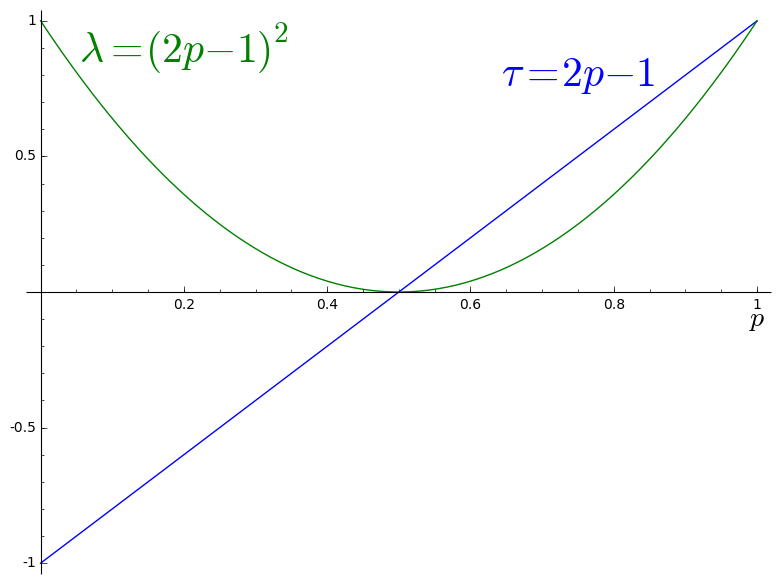
\includegraphics[scale=0.5]{figures/BC_Potenzial2.png}
\end{center}
\caption{Zusammenhang zwischen Wahrscheinlichkeit $p$,
   I/O-Korrela\-tion\index{I/O-Korrelation} $\tau$ und
   Potenzial\index{Potenzial} $\lambda$}\label{fig-bool-pot}
\end{figure}

\begin{sagecode}
\begin{verbatim}

sage: plot1 = plot(2*x-1, (x,0,1))
sage: plot2 = plot((2*x - 1)**2, (x,0,1), color = 'green')
sage: xlabel = text('$p$', (1.0, -0.1), fontsize = 20, color = 'black')
sage: legend1 = text('$\tau = 2p - 1$', (0.75,0.8), fontsize = 30)
sage: legend2 = text('$\lambda = (2p - 1)^2$', (0.2,0.9), fontsize = 30,\\
        color = 'green')
sage: show(plot1 + plot2 + xlabel + legend1 + legend2)
\end{verbatim}
\caption{Plot von I/O-Korrelation\index{I/O-Korrelation} und
   Potenzial\index{Potenzial}}\label{Sage-code-bool-pot}
\end{sagecode}

Der Schlüssel $k$ ist allerdings das Ziel des Angriffs und die
Wahrscheinlichkeit $p_{F,\alpha,\beta,\kappa}(k)$ in der
Angriffssituation unbekannt. Für die Kryptoanalyse ist es daher
angebracht, die Wahrscheinlichkeit einer linearen Relation noch
über alle Schlüssel zu mitteln:
\begin{equation}\label{eq-bool-avrg}
   p_{F,\alpha,\beta,\kappa} := \frac{1}{2^{n+l}}
      \#\{(a,k) \in \F_2^n \times \F_2^l \:|\:
           \kappa(k) = \alpha(a) + \beta(F(a,k)) \}.
\end{equation}
Diese Größe ist, zumindest theoretisch, wenn man die Effizienzfrage
außer Acht lässt, allein aus der Definition der Chiffre $F$ bestimmbar.
Ihre Bestimmung läuft allerdings auf eine Exhaustion aller Klartexte
und Schlüssel hinaus und ist daher bei einer realen Chiffre mit
genügend großen Blocklängen oft wirklich nur theoretisch.
Auch hierfür werden  I/O-Korrelation\index{I/O-Korrelation} und
Potenzial\index{Potenzial} definiert:
\[
   \tau_{F,\alpha,\beta,\kappa} := 2 p_{F,\alpha,\beta,\kappa} - 1,
\]
\[
   \lambda_{F,\alpha,\beta,\kappa} := \tau_{F,\alpha,\beta,\kappa}^2.
\]

Shamir\index{Shamir, Adi}\footnote{%
  Adi Shamir, israelischer Kryptologe, Miterfinder des RSA-Verfahrens,
  $~^{\ast}$6.7.1952.
}
bemerkte schon 1985, dass es überzufällige lineare
Relationen\index{lineare Relation}\index{Relation!linear}
für die S-Boxen des DES\index{DES}-Verfahrens gibt. Es dauerte allerdings weitere
sieben Jahre, bis es Matsui\index{Matsui, Mitsuru}\footnote{%
  Mitsuru Matsui, japanischer Kryptologe, $~^{\ast}$16.9.1961.
}
(nach ersten Versuchen von Gilbert und Chassé 1990 mit der Chiffre FEAL)
gelang, diese Beobachtung systematisch
auszunutzen. Er ging zur Schätzung\index{Maximum-Likelihood-Schätzung}\footnote{%
   Das ist eine sogenannte Maximum-Likelihood-Schätzung, d.\,h.,
   man entscheidet sich für diejenige von mehreren Hypothesen (hier
   sind es nur zwei), unter deren Annahme das Beobachtungsergebnis
   die höchste Wahrscheinlichkeit hat.
} von $\kappa(k)$ wie folgt vor
(im Fall $p_{F,\alpha,\beta,\kappa} > \frac{1}{2}$, sonst muss man
bei der Entscheidung die Werte $0$ und $1$ vertauschen\footnote{%
  Im Fall $p_{F,\alpha,\beta,\kappa} = \frac{1}{2}$ ist die
  Methode in dieser Form unbrauchbar.
}):
\begin{enumerate}
	\item {\bf [Sammelphase]} Man sammelt $N$ Klartext-Geheimtextpaare
	  $(a_1,c_1), \ldots, (a_N,c_N)$.

	\item {\bf [Auszählung]} Man bestimmt die Anzahl
\[
    t := \# \{i = 1, \ldots, N \:|\: \alpha(a_i) + \beta(c_i) = 0\}.
\]

	\item {\bf [Mehrheitsentscheidung]} aufgrund von $t$:
	  \begin{itemize}
	    \item Ist $t > \frac{N}{2}$, schätzt man $\kappa(k) = 0$.
	    \item Ist $t < \frac{N}{2}$, schätzt man $\kappa(k) = 1$.
	  \end{itemize}
\end{enumerate}
Der Fall $t = \frac{N}{2}$ ist unergiebig, kommt aber selten vor -- man
entscheidet zufällig zwischen $0$ und $1$ oder gibt eine entsprechende
Rückmeldung\footnote{%
   am besten beides wie im SageMath-Beispiel~\ref{Sage-code-bool-mats}
}. Im SageMath-Beispiel~\ref{Sage-code-bool-mats}
steht der Programmcode, eine konkrete Anwendung folgt gleich als Beispiel
im nächsten Unterabschnitt.

\begin{sagecode}
\begin{verbatim}

def Matsui_Test(a, b, pc, compl = False):
  """Matsui's test for linear cryptanalysis"""
  N = len(pc)
  results = []
  for pair in pc:
    ax = binScPr(a,pair[0])
    by = binScPr(b,pair[1])
    result = (ax + by) % 2
    results.append(result)
  t = 0
  for bb in results:
    if bb == 0:
      t = t + 1
  if 2*t > N:
    if compl:
      return [t,1,True]
    else:
      return [t,0,True]
  elif 2*t_0 < N:
    if compl:
      return [t,0,True]
    else:
      return [t,1,True]
  else:
    return [t,randint(0,1),False]
\end{verbatim}
\caption{Matsui-Test\index{Matsui-Test}. Die Linearformen sind {\tt a} für $\alpha$ und
   {\tt b} für $\beta$. Die Liste {\tt pc} enthält {\tt N} Paare von Klartext
   und Geheimtext. Der Boolesche Wert {\tt compl} gibt an, ob das
   als Ergebnis geschätzte Bit invertiert werden soll. Die Ausgabe
   ist ein Tripel aus der Anzahl {\tt t} der gezählten Nullen,
   dem geschätzten Bit und einem Booleschen Wert, der angibt, ob das
   Bit deterministisch bestimmt ({\tt True}) oder im Grenzfall
   zufällig bestimmt ({\tt False}) wurde. Verwendet wird die Funktion
   {\tt binScPr} aus dem SageMath-Beispiel~\ref{Sage-code-bool-div-bbl}
   im Anhang~\ref{ss-bool-conv}.}\label{Sage-code-bool-mats}
\end{sagecode}

Wenn man eine lineare Relation\index{lineare Relation}\index{Relation!linear}
mit hinreichend großem Potenzial\index{Potenzial}, d.\,h.
hinreichend weit von $\frac{1}{2}$ abweichender Wahrscheinlichkeit, erwischt hat,
wird die Erfolgswahrscheinlichkeit dieses Verfahrens bei hinreichend
großem $N$ gut sein. Das erlaubt dann, die Anzahl der unbekannten
Schlüsselbits durch Elimination\index{Elimination} um 1 zu verringern.

Als theoretisches Ergebnis aus diesen Überlegungen
werden wir einen Zusammenhang zwischen der Anzahl $N$ von
benötigten Klartextblöcken und der Erfolgswahrscheinlichkeit erhalten,
siehe Tabelle~\ref{tab-bool-N}.

Je mehr solcher linearen Relationen die Angreiferin mit genügend hoher
Gewissheit findet, desto stärker kann sie die Größe des Schlüsselraums
einschränken, bis schließlich eine Exhaustion\index{Exhaustion} über die noch in Frage
kommenden Schlüssel in den Bereich des Machbaren rückt. Ein konkretes
Beispiel in Abschnitt~\ref{ss-bool-mini} wird dies illustrieren.

\subsubsection*{Beispiel}

Für ein konkretes Beispiel mit $n = l = 4$ betrachten wir die
Boolesche Abbildung\footnote{%
   $f$ ist nebenbei bemerkt die S-Box\index{S-Box} $\mathrm{S}_0$
   von {\sc Lucifer}\index{Lucifer},
   das um 1970 als Vorgänger-Verfahren von DES\index{DES} entwickelt wurde.
} $f$, die durch die Wertetabelle~\ref{tab-bool-A1}
gegeben ist, und bilden damit die Bitblock-Chiffre
(s.\,a. Abbildung~\ref{fig-bool-bsp0})
\[
    F\!: \F_2^4 \times \F_2^4 \longrightarrow \F_2^4, \quad
    F(a,k) := f(a + k).
\]
Das SageMath-Beispiel~\ref{Sage-code-Luc-S0} definiert diese Boolesche
Abbildung $f$ unter dem Namen {\tt S0}
und verwendet die Klassen {\tt BoolF} und {\tt BoolMap} aus dem
Anhang~\ref{ss-bool-class}. Dabei geben die Spalten der (impliziten)
definierenden Matrix genau die Werte der Abbildung an, wie man sie auch
in Tabelle~\ref{tab-bool-A1} in der Spalte $y = f(x)$ wiederfindet.
(D.\,h., das SageMath-Beispiel~\ref{Sage-code-Luc-S0} und die
Tabelle~\ref{tab-bool-A1} enthalten äquivalente Definitionen der
Abbildung $f$.)
Eine exemplarische Evaluation illustriert das (für die dritte Spalte,
entsprechend dem Argument {\tt 0010}).

\begin{sagecode}
\begin{verbatim}

f1 = BoolF([1,1,0,1,1,1,1,0,0,0,0,0,1,0,0,1])
f2 = BoolF([1,1,1,0,1,1,0,0,0,1,0,0,0,1,1,0])
f3 = BoolF([0,1,1,1,1,0,1,0,1,1,1,0,0,0,0,0])
f4 = BoolF([0,1,1,0,0,1,1,0,0,0,1,1,1,0,1,0])
S0 = BoolMap([f1,f2,f3,f4])
# Sample evaluation
sage: S0.valueAt([0,0,1,0])
[0, 1, 1, 1]
\end{verbatim}
\caption{Eine Boolesche Abbildung (S-Box $\mathrm{S}_0$ von
   {\sc Lucifer})}\label{Sage-code-Luc-S0}
\end{sagecode}

Wir verschlüsseln mit dem Schlüssel $k =$ \verb:1000:, den wir später zur
Probe angreifen wollen. Für eine lineare Relation betrachten wir die
Linearformen
\[
     \alpha(a) = a_4, \quad \beta(c) = c_1 + c_2 + c_4, \quad \kappa(k) = k_4;
\]
wir werden in Abschnitt~\ref{ss-bool-bsp1} sehen, dass mit diesen
Linearformen die Relation
$\kappa(k) = \alpha(a) + \beta(c)$ für $F$ eine Wahrscheinlichkeit
deutlich $> \frac{1}{2}$ hat. Tabelle~\ref{tab-bool-mats} zeigt die
Verschlüsselung dreier Klartexte $a$, die wir später als bekannte
Klartexte annehmen wollen. Die Werte für $c$ wurden aus der
Wertetabelle~\ref{tab-bool-A1} abgelesen. Die Anzahl $t$ der
beobachteten Werte $0$ von $\alpha(a)$ + $\beta(c)$ ist $t = 2$.
Die Mehrheitsentscheidung führt also zu der Schätzung $k_4 = 0$
(von der wir wissen, dass sie korrekt ist).

\begin{table}
\begin{center}
\begin{tabular}{|c|c|c|c|} \hline
       $x$   & $y=f(x)$& $\alpha(x) = x_4$ & $\beta(y) = y_1+y_2+y_4$ \\ \hline
     0 0 0 0 & 1 1 0 0 &   0   &  0  \\
     0 0 0 1 & 1 1 1 1 &   1   &  1  \\
     0 0 1 0 & 0 1 1 1 &   0   &  0  \\
     0 0 1 1 & 1 0 1 0 &   1   &  1  \\
     0 1 0 0 & 1 1 1 0 &   0   &  0  \\
     0 1 0 1 & 1 1 0 1 &   1   &  1  \\
     0 1 1 0 & 1 0 1 1 &   0   &  0  \\
     0 1 1 1 & 0 0 0 0 &   1   &  0  \\
     1 0 0 0 & 0 0 1 0 &   0   &  0  \\
     1 0 0 1 & 0 1 1 0 &   1   &  1  \\
     1 0 1 0 & 0 0 1 1 &   0   &  1  \\
     1 0 1 1 & 0 0 0 1 &   1   &  1  \\
     1 1 0 0 & 1 0 0 1 &   0   &  0  \\
     1 1 0 1 & 0 1 0 0 &   1   &  1  \\
     1 1 1 0 & 0 1 0 1 &   0   &  0  \\
     1 1 1 1 & 1 0 0 0 &   1   &  1  \\ \hline
\end{tabular}
\end{center}
\caption{Wertetabelle einer Booleschen Abbildung
  $f\!: \F_2^4 \longrightarrow \F_2^4$ und zwei Linearformen}\label{tab-bool-A1}
\end{table}

\begin{table}
\begin{center}
\begin{tabular}{|c|c|c||ccc|}\hline
   $a$  & $a+k$ & $c$  & $\alpha(a)$ & $\beta(c)$ & $\alpha(a)$ + $\beta(c)$ \\
   \hline
   0010 & 1010  & 0011 &     0       &      1     &             1            \\
   0101 & 1101  & 0100 &     1       &      1     &             0            \\
   1010 & 0010  & 0111 &     0       &      0     &             0            \\
   \hline
\end{tabular}
\end{center}
\caption{Schätzung eines Schlüsselbits nach Matsui unter Verwendung von drei
   bekannten Klartexten}\label{tab-bool-mats}
\end{table}

Das war mit dem Bleistift auf Papier ganz leicht auszuzählen. Dennoch
ist der Nachvollzug in SageMath im Hinblick auf kompliziertere Beispiele
instruktiv. Das geschieht im SageMath-Beispiel~\ref{Sage-code-Mats-Expl}.
Dabei wird die Funktion {\tt xor}\index{XOR} aus dem
SageMath-Beispiel~\ref{Sage-code-bool-div-bbl} im Anhang~\ref{ss-bool-conv}
sowie die im SageMath-Beispiel~\ref{Sage-code-Luc-S0}
definierte Abbildung {\tt S0} verwendet. Das Ergebnis \mbox{\tt [2, 0, True]}
besagt, dass $2$ Nullen unter den ausgezählten Werten waren, was zur
Mehrheitsentscheidung $0$ führt, die (wegen {\tt True}) nicht durch
zufällige Auslosung bei Gleichstand ermittelt wurde.

\begin{sagecode}
\begin{verbatim}

sage: k = [1,0,0,0]
sage: alpha = [0,0,0,1]
sage: beta = [1,1,0,1]
sage: plist = [[0,0,1,0],[0,1,0,1],[1,0,1,0]]
sage: xlist = []
sage: xclist = []
sage: pclist = []
sage: for i in range(0,len(plist)):
....:     x = xor(plist[i],k)
....:     xlist.append(x)
....:
sage: xlist
[[1, 0, 1, 0], [1, 1, 0, 1], [0, 0, 1, 0]]
sage: for i in range(0,len(plist)):
....:     val = S0.valueAt(xlist[i])
....:     xclist.append([xlist[i],val])
....:     pclist.append([plist[i],val])
....:
sage: Matsui_Test(alpha,beta,pclist,False)
[2, 0, True]
\end{verbatim}
\caption{Ein Beispiel für den Matsui-Test\index{Matsui-Test}}\label{Sage-code-Mats-Expl}
\end{sagecode}

\noindent Damit das Verfahren im allgemeinen Fall Erfolg verspricht, sind
folgende Fragen zu klären:
\begin{enumerate}
	\item Wie findet man lineare
        Relationen\index{lineare Relation}\index{Relation!linear}
        von möglichst auffälliger
        Wahrscheinlichkeit? Insbesondere im Hinblick darauf, dass die
        Auswertung der Formel~(\ref{eq-bool-avrg}) am Effizienzproblem
        scheitert.
     \item Da Bitblock-Chiffren\index{Bitblock-Chiffre} meistens aus
        vielen Runden\index{Runde} zusammengesetzt sind, fragt man weiter:
	\begin{enumerate}
	  \item Wie findet man bei einer iterierten Bitblock-Chiffre
	    brauchbare lineare Relationen für die Rundenfunktion?
	  \item Wie setzt man diese über die Runden hinweg zu linearen Relationen
	    für die ganze Chiffre zusammen?
	  \item Wie bestimmt man die Wahrscheinlichkeit einer zusammengesetzten
	    linearen Relation für die ganze Chiffre aus der für die einzelnen
	    Runden?
	\end{enumerate}
\end{enumerate}

\noindent Die Antwort auf die erste Frage und Teil (a) der zweiten heißt:
Aus dem linearen Profil\index{lineares Profil}\index{Profil!linear},
siehe Abschnitt~\ref{ss-bool-lpr}. Die anschließenden
Teilfragen führen zur Untersuchung von linearen
Pfaden\index{linearer Pfad}\index{Pfad!linear},
siehe Abschnitt~\ref{ss-bool-path}, und zur Kumulation von
Wahrscheinlichkeiten, siehe Satz~\ref{thm-bool-rrnd}. Für (c) kommt
dabei letztendlich eine brauchbare Faustregel heraus.

\subsection{Beispiel A: Eine Einrunden-Chiffre}\label{ss-bool-bsp1}

Es werden Beispiele betrachtet, die als ernsthafte Blockchiffren viel
zu einfach sind, aber das Prinzip der linearen
Kryptoanalyse\index{lineare Kryptoanalyse}\index{Kryptoanalyse!linear}
anschaulich und nachvollziehbar demonstrieren. Dabei werden stets
Rundenfunktionen der Gestalt $f(a+k)$ betrachtet, d.\,h., der Schlüssel
bzw. ein $n$-bittiger Teil davon wird vor der Anwendung einer bijektiven
S-Box $f\!: \F_2^n \longrightarrow \F_2^n$ binär auf den Klartext
aufaddiert\footnote{%
   Das ist zwar eine sehr spezielle Art, den Schlüssel in das Verfahren
   einzubringen, aber dennoch realistisch. Die paradigmatischen
   Beispiel-Chiffren {\sc Lucifer}\index{Lucifer}, DES\index{DES}
   und AES\index{AES} verfahren so.
   Bei AES \cite{DaRi2002} heißt das \glqq key-alternating cipher structure\grqq.
}. Das einfachste denkbare Modell, die Verschlüsselung nach der
Vorschrift
\[
   c = f(a+k)
\]
wie im Beispiel des Abschnitts~\ref{ss-bool-lka},
siehe Abbildung~\ref{fig-bool-bsp0}\footnote{%
  In den grafischen Darstellungen hier und später wird die Abbildung
  $f$ auf der elementweisen Ebene durch die S-Box S repräsentiert.
},
ist dabei witzlos, da bei bekanntem\index{bekannter Klartext}\index{Klartext!bekannt}
Klartext die Gleichung nach dem
Schlüssel $k$ auflösbar ist\footnote{%
  Die Umkehrabbildung $f^{-1}$ wird hier als der Angreiferin
  bekannt angenommen. Sie ist ja Teil des Algorithmus zur Entschlüsselung.
  Einweg-Verschlüsselungen\index{Einweg-Verschlüsselung},
  bei denen $f^{-1}$ aus $f$ nicht effizient
  herleitbar ist, bilden ein anderes Kapitel der Kryptographie.
}:
\[
   k = f^{-1}(c) + a.
\]

\begin{figure}
\begin{center}
\begin{picture}(268,68)(0,0)
% Mengen
   \put(11,14){$\F_2^n$}
   \put(28,17){\vector(1,0){34}}
   \put(66,14){$\F_2^n$}
   \put(54,26){$\bigoplus$}
   \put(66,54){$\F_2^n$}
   \put(71,51){\vector(0,-1){28}}
   \put(83,17){\vector(1,0){34}}
   \put(94,20){$f$}
   \put(123,14){$\F_2^n$}

% Elemente
   \put(154,14){$a$}
   \put(165,17){\vector(1,0){28}}
   \put(165,14){\line(0,1){6}}
   \put(197,14){$b$}
   \put(197,54){$k$}
   \put(199,51){\vector(0,-1){28}}
   \put(197,51){\line(1,0){6}}
   \put(205,17){\vector(1,0){40}}
   \put(205,14){\line(0,1){6}}
   \put(214,14){\fcolorbox{black}{yellow}{S}}
   \put(251,14){$c$}

% Rahmen
   \put(0,0){\line(1,0){268}}
   \put(0,68){\line(1,0){268}}
   \put(0,0){\line(0,1){68}}
   \put(268,0){\line(0,1){68}}
\end{picture}
\end{center}
\caption{Ein (viel) zu einfaches Beispiel}\label{fig-bool-bsp0}
\end{figure}

\begin{figure}
\begin{center}
\begin{picture}(208,137)(0,0)
% Mengen
   \put(11,83){$\F_2^n$}
   \put(28,85){\vector(1,0){34}}
   \put(66,83){$\F_2^n$}
   \put(54,94){$\bigoplus$}
   \put(66,124){$\F_2^n$}
   \put(71,120){\vector(0,-1){28}}
   \put(83,85){\vector(1,0){34}}
   \put(94,88){$f$}
   \put(125,83){$\F_2^n$}
   \put(140,85){\vector(1,0){34}}
   \put(179,124){$\F_2^n$}
   \put(185,120){\vector(0,-1){28}}
   \put(168,94){$\bigoplus$}
   \put(179,83){$\F_2^n$}

% Elemente
   \put(23,14){$a$}
   \put(34,17){\vector(1,0){28}}
   \put(34,14){\line(0,1){6}}
   \put(71,14){$b$}
   \put(68,54){$k^{(0)}$}
   \put(74,51){\vector(0,-1){28}}
   \put(71,51){\line(1,0){6}}
   \put(80,17){\vector(1,0){40}}
   \put(80,14){\line(0,1){6}}
   \put(91,14){\fcolorbox{black}{yellow}{S}}
   \put(128,14){$b'$}
   \put(179,54){$k^{(1)}$}
   \put(185,51){\vector(0,-1){28}}
   \put(182,51){\line(1,0){6}}
   \put(142,17){\vector(1,0){28}}
   \put(142,14){\line(0,1){6}}
   \put(182,14){$c$}

% Rahmen
   \put(0,0){\line(1,0){208}}
   \put(0,137){\line(1,0){208}}
   \put(0,0){\line(0,1){137}}
   \put(208,0){\line(0,1){137}}
\end{picture}
\end{center}
\caption{Beispiel A: Eine Einrunden-Chiffre}\label{fig-bool-bspA}
\end{figure}

\begin{figure}
\begin{center}
\begin{picture}(85,68)(0,0)
   \put(6,48){$\F_2^n$}
   \put(23,51){\vector(1,0){40}}
   \put(40,54){$f$}
   \put(68,48){$\F_2^n$}
   \put(40,9){$\F_2$}
   \put(17,43){\vector(1,-1){23}}
   \put(17,26){$\alpha$}
   \put(68,43){\vector(-1,-1){23}}
   \put(60,26){$\beta$}
   \put(38,31){$\stackrel{p}{\approx}$}

% Rahmen
   \put(0,0){\line(1,0){85}}
   \put(0,68){\line(1,0){85}}
   \put(0,0){\line(0,1){68}}
   \put(85,0){\line(0,1){68}}
\end{picture}
\end{center}
\caption{Diagramm für eine "`approximative"' lineare
   Relation\index{lineare Relation}\index{Relation!linear}}\label{fig-bool-appr}
\end{figure}

Dieser einfache Angriff wird bei dem etwas komplizierteren Beispiel A mit
\[
   c = f(a+k^{(0)}) + k^{(1)}
\]
verhindert (siehe Abbildung~\ref{fig-bool-bspA}); hier ist der Ansatz der linearen
Kryptoanalyse\index{lineare Kryptoanalyse}\index{Kryptoanalyse!linear}
bereits sinnvoll: Sei $(\alpha,\beta)$ ein Paar von Linearformen\index{Linearform}
mit
\begin{equation}\label{eq-bool-prob}
     \beta\circ f(x) \stackrel{p}{\approx} \alpha(x),
\end{equation}
wobei das Symbol $\stackrel{p}{\approx}$ zu lesen ist als
"`gleich mit Wahrscheinlichkeit $p$"', also
\[
     p = p_{f,\alpha,\beta} :=
     \frac{1}{2^{n}} \cdot \#\{x \in \F_2^n \:|\: \beta\circ f(x) = \alpha(x) \}.
\]
Repräsentiert wird die Formel~(\ref{eq-bool-prob}) durch das Diagramm in
Abbildung~\ref{fig-bool-appr}. Die Linearform $\kappa$ der
allgemeinen Theorie tritt hier nicht explizit auf: Da die
Schlüsselbits auf Klartext und ("`intermediären"') Geheimtext einfach
aufaddiert werden, ist $\kappa = \alpha$ für $k^{(0)}$ und $\kappa = \beta$
für $k^{(1)}$, also $\kappa(k^{(0)}, k^{(1)}) = \alpha(k^{(0)}) + \beta(k^{(1)})$.

Wie hängt das mit der allgemeinen Situation aus Abschnitt~\ref{ss-bool-lka}
zusammen? Für das Beispiel~A ist
\begin{itemize}
   \item die Schlüssellänge $l = 2n$, der Schlüsselraum ist $\F_2^{2n}$, und
      Schlüssel haben die Gestalt $k = (k^{(0)},k^{(1)})$ mit $k^{(0)}, k^{(1)} \in \F_2^n$.
   \item Die Chiffre ist durch die Abbildung
\[
     F\!: \F_2^n \times \F_2^n \times \F_2^n \longrightarrow \F_2^n,
     \quad (a, k^{(0)}, k^{(1)}) \mapsto f(a + k^{(0)}) + k^{(1)},
\]
      definiert.
   \item Die Linearform $\kappa\!: \F_2^n \times \F_2^n \longrightarrow \F_2$
      ist durch $\kappa(k^{(0)},k^{(1)}) = \alpha(k^{(0)}) + \beta(k^{(1)})$ gegeben.
\end{itemize}
Die Wahrscheinlichkeit einer linearen Relation für einen festen
Schlüssel \mbox{$k = (k^{(0)},k^{(1)})$} ist damit
\begin{eqnarray*}
    p_{F,\alpha,\beta,\kappa}(k) & = & \frac{1}{2^n} \cdot
      \#\{a \in \F_2^n \:|\: \kappa(k) = \alpha(a) + \beta(F(a,k)) \} \\
     & = & \frac{1}{2^n} \cdot
      \#\{a \in \F_2^n \:|\: \alpha(k^{(0)}) + \beta(k^{(1)}) = \alpha(a) + \beta(f(a + k^{(0)}) + k^{(1)}) \} \\
     & = & \frac{1}{2^n} \cdot
      \#\{a \in \F_2^n \:|\: \alpha(k^{(0)}) = \alpha(a) + \beta(f(a + k^{(0)})) \},
\end{eqnarray*}
da $\beta(k^{(1)})$ auf beiden Seiten der Gleichung innerhalb der Mengenklammern
vorkommt und daher einfach weggelassen werden kann.

Dieser Ausdruck ist unabhängig von $k^{(1)}$, und an der leicht umgeformten
Gleichung
\[
     p_{F,\alpha,\beta,\kappa}(k) = \frac{1}{2^n} \cdot
      \#\{a \in \F_2^n \:|\: \alpha(a + k^{(0)}) = \beta(f(a + k^{(0)})) \}
\]
sieht man, dass er für alle $k^{(0)}$ den gleichen Wert hat, da bei festem
$k^{(0)}$ mit $a$ auch $a + k^{(0)}$ ganz $\F_2^n$ durchläuft. Dieser Wert
muss daher mit dem Mittelwert über alle $k$ übereinstimmen:
\[
     p_{F,\alpha,\beta,\kappa}(k) = p_{F,\alpha,\beta,\kappa} = \frac{1}{2^n} \cdot
      \#\{x \in \F_2^n \:|\: \alpha(x) = \beta(f(x)) \} = p.
\]
Mit dieser Überlegung ist gezeigt:

\begin{satz}
    In der Situation des Beispiels~A nimmt die Wahrscheinlichkeit $p_{F,\alpha,\beta,\kappa}(k)$
    für jeden Schlüssel $k \in \F_2^{2n}$ den gleichen Wert
\[
     p = \frac{1}{2^n} \cdot \#\{x \in \F_2^n \:|\: \alpha(x) = \beta(f(x)) \}
\]
   an, insbesondere ist $p$ auch der Mittelwert nach Gleichung~(\ref{eq-bool-avrg}).
\end{satz}

Mit den Bezeichnungen aus Abbildung~\ref{fig-bool-bspA} gilt nun
\begin{align*}
   \beta(c) & = \beta(b' + k^{(1)}) = \beta(b') + \beta(k^{(1)}) \\
            & \stackrel{p}{\approx} \alpha(b) + \beta(k^{(1)})
                   = \alpha(a + k^{(0)}) + \beta(k^{(1)})
                        = \alpha(a) + \alpha(k^{(0)}) + \beta(k^{(1)}).
\end{align*}
Als lineare Relation\index{lineare Relation}\index{Relation!linear}
für die Bits des Schlüssels $k = (k^{(0)},k^{(1)})$ erhalten wir
\[
   \alpha(k^{(0)}) + \beta(k^{(1)}) \stackrel{p}{\approx} \alpha(a) + \beta(c).
\]
Ein analoger Schluss lässt sich für die komplementäre Relation
\[
   \beta\circ f(x) \stackrel{1-p}{\approx} \alpha(x) + 1
\]
durchführen. Insgesamt ist damit gezeigt:

\begin{satz}
  Im Beispiel~A sei $(\alpha,\beta)$ ein Paar von Linearformen\index{Linearform} für $f$
  mit der Wahrscheinlichkeit $p$ wie in Formel~(\ref{eq-bool-prob}).
  Dann ist $\hat{p} =$ \mbox{$\max\{p, 1-p\}$} die Erfolgswahrscheinlichkeit für
  die Bestimmung eines Schlüsselbits aus {\em einem} bekannten
  Klartext\index{bekannter Klartext}\index{Klartext!bekannt}
  durch diese lineare Relation\index{lineare Relation}\index{Relation!linear}.
\end{satz}

\subsubsection*{Beispiel}

Nehmen wir als konkretes Beispiel $n = 4$ und für $f$ wieder die S-Box
$\mathrm{S}_0$ von {\sc Lucifer}\index{Lucifer}. Die beiden rechten Spalten der
Tabelle~\ref{tab-bool-A1} zeigen, dass die durch $(\alpha,\beta)$ mit $\alpha(x) = x_4$
und $\beta(y) = y_1+y_2+y_4$ definierte lineare Relation die Wahrscheinlichkeit
$p_{f,\alpha,\beta} = \frac{14}{16} = \frac{7}{8}$ hat\footnote{%
  Deren Größe ist ein starkes Indiz dafür, dass die Designer von
  {\sc Lucifer}\index{Lucifer} die lineare
  Kryptoanalyse\index{lineare Kryptoanalyse}\index{Kryptoanalyse!linear}
  noch nicht kannten.
}.

Die konkreten Rundenschlüssel\index{Rundenschlüssel} seien
$k^{(0)} =$ \verb:1000: und $k^{(1)} =$ \verb:0001:.
Die Tabelle~\ref{tab-bool-linrel} über alle $16$ möglichen
Klartexte zeigt, dass $\alpha(a)+\beta(c)$ den Wert $1 =\alpha(k^{(0)}) + \beta(k^{(1)})$
für die Summe der Schlüsselbits genau $14$-mal annimmt, wie es sein soll.

\begin{table}
\begin{center}
\begin{tabular}{|cccc|c|} \hline
  $a$  & $b$  & $b'$ & $c$  & $\alpha(a)+\beta(c) = a_4 + c_1 + c_2 + c_4$ \\ \hline
  0000 & 1000 & 0010 & 0011 & 1 \\
  0001 & 1001 & 0110 & 0111 & 1 \\
  0010 & 1010 & 0011 & 0010 & 0 \\
  0011 & 1011 & 0001 & 0000 & 1 \\
  0100 & 1100 & 1001 & 1000 & 1 \\
  0101 & 1101 & 0100 & 0101 & 1 \\
  0110 & 1110 & 0101 & 0100 & 1 \\
  0111 & 1111 & 1000 & 1001 & 1 \\
  1000 & 0000 & 1100 & 1101 & 1 \\
  1001 & 0001 & 1111 & 1110 & 1 \\
  1010 & 0010 & 0111 & 0110 & 1 \\
  1011 & 0011 & 1010 & 1011 & 1 \\
  1100 & 0100 & 1110 & 1111 & 1 \\
  1101 & 0101 & 1101 & 1100 & 1 \\
  1110 & 0110 & 1011 & 1010 & 1 \\
  1111 & 0111 & 0000 & 0001 & 0 \\
  \hline
\end{tabular}
\end{center}
\caption{Eine lineare Relation für die Schlüsselbits ($b$ entsteht aus $a$ durch Addition
   von $k^{(0)}$, also ``Umkippen'' des ersten Bits, $b'$ aus $b$ durch Anwendung
   von $f$, $c$ aus $b'$ durch Addition von $k^{(1)}$.}\label{tab-bool-linrel}
\end{table}

Wie groß ist nun die Erfolgswahrscheinlichkeit $p_N$ dafür, diesen Wert
richtig zu schätzen, wenn man $N = 1, 2, \ldots$ zufällige bekannte
Klartexte\index{bekannter Klartext}\index{Klartext!bekannt}
aus der Menge der $2^n$ möglichen zur Verfügung hat (zu gegebenen festen
Linearformen $\alpha$ und $\beta$ mit $p = p_{f,\alpha,\beta}$)? Das ist genau
eine konkrete Einkleidung der Fragestellung der hypergeometrischen Verteilung,
und daher gilt
(ohne Beweis und ohne Erklärung der hypergeometrischen
Verteilung\index{hypergeometrische Verteilung}\index{Verteilung!hypergeometrisch}):

\begin{satz}
  Im Beispiel A sei $(\alpha,\beta)$ ein Paar von Linearformen, das
  eine lineare Relation für $f$ mit der Wahrscheinlichkeit $p$ definiert.
  Dann ist die Erfolgswahrscheinlichkeit für die Bestimmung eines
  Schlüsselbits aus $N$ bekannten Klartexten durch diese lineare
  Relation\index{lineare Relation}\index{Relation!linear}
  gerade die kumulierte Wahrscheinlichkeit $p_N = p_N^{(s)}$ der
  hypergeometrischen Verteilung zu den Parametern $2^n$, $s = \hat{p}\cdot 2^n$
  und $N$ mit $\hat{p} = \max\{p, 1-p\}$.
\end{satz}

Verlässt man die exakte Mathematik und geht, wie oft in der angewandten Statistik,
zu asymptotischen Näherungsformeln über, so kann man unter den (sehr vage
formulierten) Voraussetzungen
"`$p$ nicht zu weit von $\frac{1}{2}$ entfernt, $N \ll 2^n$, aber $N$ nicht
zu klein,"' die hypergeometrische Verteilung\index{hypergeometrische
Verteilung}\index{Verteilung!hypergeometrisch} durch die
Normalverteilung\index{Normalverteilung} approximieren und erhält
\begin{equation}\label{equ-bool-N}
  p_N \approx \frac{1}{\sqrt{2\pi}} \cdot
                      \int_{-\infty}^{\sqrt{N\lambda}} e^{-t^2/2}\,dt,
\end{equation}
wobei $\lambda = (2p - 1)^2$ das Potenzial\index{Potenzial} der linearen Relation ist.
Zusammen mit den bekannten Werten für die Normalverteilung\footnote{%
   Man kann statt mit der Approximation durch die Normalverteilung auch direkt
   mit der hypergeometrischen
   Verteilung\index{hypergeometrische Verteilung}\index{Verteilung!hypergeometrisch}
   rechnen. Dann erhält man,
   besonders bei kleinem $N$, einen genaueren Wert, aber keine so
   einfache geschlossene Formel wie (\ref{equ-bool-N}).
} ergibt das die
Tabelle~\ref{tab-bool-N}. D.\,h., um eine Erfolgswahrscheinlichkeit von etwa
$95\%$ zu erreichen, braucht man $N \approx \frac{3}{\lambda}$ bekannte
Klartexte\index{bekannter Klartext}\index{Klartext!bekannt}.
Im obigen konkreten Beispiel war $p = \frac{7}{8}$, also $\lambda = \frac{9}{16}$,
und die Zahl der nötigen bekannten Klartexte für die $95$-prozentige
Erfolgswahrscheinlichkeit ist nach der Formel $N \approx 5$. Wir waren,
siehe Tabelle~\ref{tab-bool-mats}, schon mit $N = 3$ erfolgreich gewesen;
das ist nicht sehr überraschend, denn wie wir jetzt sehen, war
die Erfolgswahrscheinlichkeit dafür immerhin knapp 90\% (hier ist nämlich
$N\lambda = \frac{27}{16} \approx 1,68\ldots$)\footnote{%
   Hier wird man die Voraussetzung "`$N$ nicht zu klein"' der Approximation
   durch die Normalverteilung\index{Normalverteilung} zu Recht anzweifeln müssen.
   In der Tat kann man leicht die exakten Werte für die hypergeometrische
   Verteilung\index{hypergeometrische Verteilung}\index{Verteilung!hypergeometrisch}
   bestimmen:
   Zieht man aus einer Urne mit $16$ Kugeln, von denen $14$ schwarz und
   $2$ weiß sind, zufällig $3$ Kugeln, so werden diese mit Wahrscheinlichkeit
   $\frac{26}{40}$ alle drei schwarz sein, und mit Wahrscheinlichkeit
   $\frac{13}{40}$ zwei davon schwarz und eine weiß, also mit Wahrscheinlichkeit
   $\frac{39}{40} = 97,5\%$ mindestens zwei schwarz. Das ist also deutlich
   mehr als die aus der Approximationsformel~(\ref{equ-bool-N}) bestimmten 90\%.
   Die übrigen Wahrscheinlichkeiten sind $\frac{1}{40}$ für genau eine schwarze
   Kugel und $0$ für drei weiße.
}.

\begin{table}
\begin{center}
  \begin{tabular}{|c|ccccccc|} \hline
		$N\lambda$ & $1$ & $2$ & $3$ & $4$ & \ldots & $8$ & $9$ \\
		$p_N$ & $84,1\%$ & $92,1\%$ & $95,8\%$ & $97,7\%$ & \ldots &
		                      $99,8\%$ & $99,9\%$ \\ \hline
  \end{tabular}
\end{center}
\caption{Zusammenhang zwischen der Anzahl der bekannten
   Klartexte\index{bekannter Klartext}\index{Klartext!bekannt}
   und der Erfolgs\-wahr\-schein\-lich\-keit}\label{tab-bool-N}
\end{table}

\subsection{Approximationstabelle\index{Approximationstabelle},
   Korrelationsmatrix\index{Korrelationsmatrix} und lineares
   Profil\index{lineares Profil}\index{Profil!linear}}\label{ss-bool-lpr}

Die Häufigkeiten, mit denen lineare
Relationen\index{lineare Relation}\index{Relation!linear} für eine Boolesche
Abbildung\index{Boolesche Abbildung}\index{Abbildung!Boolesche}
(oder S-Box\index{S-Box}) $f\!: \F_2^n \longrightarrow \F_2^q$ gelten, werden
in einer $2^n \times 2^q$-Matrix zusammengefasst, die zu
jedem Paar von Linearformen\index{Linearform} $(\alpha,\beta)$
die Anzahl der Argumente $x$ mit $\beta\circ f(x) = \alpha(x)$ angibt und
{\bf Approximationstabelle\index{Approximationstabelle}}
genannt wird\footnote{%
   Vorsicht mit den Literatur-Referenzen: Oft wird von allen Einträgen
   noch der Wert $2^{n-1}$ abgezogen, so z.\,B. bei der SageMath-Funktion
   {\tt linear\_approximation\_matrix()}.
}\label{fn-lin-appr}.
Für die oben verwendete S-Box $\mathrm{S}_0$ von {\sc Lucifer}\index{Lucifer}
ist sie in Tabelle~\ref{tab-bool-s0} wiedergegeben. Der Eintrag $16$ in
der linken oberen Ecke besagt, dass die Relation $0 = 0$ immer, also
in allen $16$ Fällen gilt, und ist gleichzeitig der Hauptnenner, durch
den man alle Einträge teilen muss, um die Wahrscheinlichkeiten zu
erhalten; im allgemeinen Fall würde dort $2^n$ stehen. Die übrigen Einträge
in der ersten Spalte (entsprechend $\beta = 0$) sind $8$, weil jede von Null
verschiedene Linearform\index{Linearform} $\alpha$ den Wert $0$ in genau der
Hälfte aller Fälle, hier also $8$-mal, annimmt\footnote{%
   In der Sprache der Linearen Algebra\index{lineare Algebra}\index{Algebra!lineare}:
   Der Kern einer Linearform\index{Linearform} $\neq 0$
   ist ein $(n-1)$-dimensionaler Unterraum.
}. Für die erste Zeile gilt das analoge
Argument -- vorausgesetzt, $f$ ist bijektiv\footnote{%
   Im allgemeinen Fall, wo $q \neq n$ sein kann, müsste man hier
   "`balanciert\index{balanciert}"' sagen, d.\,h., alle Urbildmengen sind gleich groß.
   Das geht natürlich nur im Fall $q \leq n$ wirklich.
}.

\begin{table}
\begin{center}
\begin{tabular}{|c|cccccccccccccccc|} \hline
     & 0 & 1 & 2 & 3 & 4 & 5 & 6 & 7 & 8 & 9 &10 &11 &12 &13 &14 &15 \\ \hline
   0 &16 & 8 & 8 & 8 & 8 & 8 & 8 & 8 & 8 & 8 & 8 & 8 & 8 & 8 & 8 & 8 \\
   1 & 8 & 6 & 6 & 8 & 8 & 6 & 6 & 8 & 8 & 6 & 6 & 8 & 8 &14 & 6 & 8 \\
   2 & 8 &10 & 8 & 6 & 4 & 6 & 8 & 6 & 6 &12 & 6 & 8 &10 & 8 & 6 & 8 \\
   3 & 8 &12 &10 & 6 &12 & 8 &10 & 6 & 6 & 6 & 8 & 8 &10 &10 & 8 & 8 \\
   4 & 8 & 8 & 4 & 8 & 8 & 8 & 8 & 4 &10 & 6 & 6 & 6 &10 & 6 &10 &10 \\
   5 & 8 &10 &10 &12 & 8 &10 & 6 & 8 &10 & 8 & 4 &10 &10 & 8 & 8 & 6 \\
   6 & 8 &10 & 8 &10 & 8 &10 & 8 &10 & 8 &10 & 8 & 2 & 8 &10 & 8 &10 \\
   7 & 8 & 8 &10 & 6 & 8 & 8 & 2 & 6 & 8 & 8 &10 & 6 & 8 & 8 &10 & 6 \\
   8 & 8 & 8 & 6 &10 & 6 &10 & 8 & 8 & 4 & 8 &10 &10 &10 &10 &12 & 8 \\
   9 & 8 &10 & 8 &10 & 6 & 4 &10 & 8 & 8 & 6 & 8 & 6 & 6 & 8 &10 & 4 \\
  10 & 8 & 6 &10 & 8 & 6 & 8 & 8 &10 & 6 & 4 & 8 & 6 &12 & 6 & 6 & 8 \\
  11 & 8 &12 & 8 & 8 & 6 & 6 & 6 &10 &10 & 6 &10 &10 & 8 & 8 & 8 &12 \\
  12 & 8 & 8 &10 &10 & 6 &10 & 8 & 4 & 6 & 6 & 8 & 8 & 4 & 8 & 6 &10 \\
  13 & 8 & 6 &12 & 6 & 6 & 8 &10 & 8 &10 & 8 & 6 & 8 & 8 &10 &12 & 8 \\
  14 & 8 & 6 &10 &12 &10 & 4 & 8 & 6 & 8 &10 &10 & 8 &10 & 8 & 8 &10 \\
  15 & 8 & 8 & 8 & 8 &10 & 6 & 6 &10 & 4 & 8 & 4 & 8 & 6 & 6 &10 &10 \\ \hline
\end{tabular}
\end{center}
\caption{Approximationstabelle der S-Box $\mathrm{S}_0$ von {\sc Lucifer}\index{Lucifer} --
   Zeilen- und Spaltenindizes sind durch Zahlen repräsentierte Linearformen,
   siehe Abschnitt~\ref{ss-bool-repr}.
   Die Wahrscheinlichkeiten erhält man nach Division durch 16.}\label{tab-bool-s0}
\end{table}

\begin{table}
\begin{center}
\begin{tabular}{|c|cccccccccccccccc|} \hline
     & 0 & 1 & 2 & 3 & 4 & 5 & 6 & 7 & 8 & 9 &10 &11 &12 &13 &14 &15 \\ \hline
   0 & 1 & 0 & 0 & 0 & 0 & 0 & 0 & 0 & 0 & 0 & 0 & 0 & 0 & 0 & 0 & 0 \\
   1 & 0 &$-\frac{1}{4}$&$-\frac{1}{4}$& 0 & 0 &$-\frac{1}{4}$&$-\frac{1}{4}$& 0 & 0 &$-\frac{1}{4}$&$-\frac{1}{4}$& 0 & 0 &$\frac{3}{4}$&$-\frac{1}{4}$& 0 \\
   2 & 0 &$\frac{1}{4}$& 0 & $-\frac{1}{4}$ &$-\frac{1}{2}$& $-\frac{1}{4}$ & 0 & $-\frac{1}{4}$ & $-\frac{1}{4}$ &$\frac{1}{2}$& $-\frac{1}{4}$ & 0 &$\frac{1}{4}$& 0 & $-\frac{1}{4}$ & 0 \\
   3 & 0 &$\frac{1}{2}$&$\frac{1}{4}$& $-\frac{1}{4}$ &$\frac{1}{2}$& 0 &$\frac{1}{4}$& $-\frac{1}{4}$ & $-\frac{1}{4}$ & $-\frac{1}{4}$ & 0 & 0 &$\frac{1}{4}$&$\frac{1}{4}$& 0 & 0 \\
   4 & 0 & 0 &$-\frac{1}{2}$& 0 & 0 & 0 & 0 &$-\frac{1}{2}$&$\frac{1}{4}$& $-\frac{1}{4}$ & $-\frac{1}{4}$ & $-\frac{1}{4}$ &$\frac{1}{4}$& $-\frac{1}{4}$ &$\frac{1}{4}$&$\frac{1}{4}$\\
   5 & 0 &$\frac{1}{4}$&$\frac{1}{4}$&$\frac{1}{2}$& 0 &$\frac{1}{4}$& $-\frac{1}{4}$ & 0 &$\frac{1}{4}$& 0 &$-\frac{1}{2}$&$\frac{1}{4}$&$\frac{1}{4}$& 0 & 0 & $-\frac{1}{4}$ \\
   6 & 0 &$\frac{1}{4}$& 0 &$\frac{1}{4}$& 0 &$\frac{1}{4}$& 0 &$\frac{1}{4}$& 0 &$\frac{1}{4}$& 0 & $-\frac{3}{4}$ & 0 &$\frac{1}{4}$& 0 &$\frac{1}{4}$\\
   7 & 0 & 0 &$\frac{1}{4}$& $-\frac{1}{4}$ & 0 & 0 & $-\frac{3}{4}$ & $-\frac{1}{4}$ & 0 & 0 &$\frac{1}{4}$& $-\frac{1}{4}$ & 0 & 0 &$\frac{1}{4}$& $-\frac{1}{4}$ \\
   8 & 0 & 0 & $-\frac{1}{4}$ &$\frac{1}{4}$& $-\frac{1}{4}$ &$\frac{1}{4}$& 0 & 0 &$-\frac{1}{2}$& 0 &$\frac{1}{4}$&$\frac{1}{4}$&$\frac{1}{4}$&$\frac{1}{4}$&$\frac{1}{2}$& 0 \\
   9 & 0 &$\frac{1}{4}$& 0 &$\frac{1}{4}$& $-\frac{1}{4}$ &$-\frac{1}{2}$&$\frac{1}{4}$& 0 & 0 & $-\frac{1}{4}$ & 0 & $-\frac{1}{4}$ & $-\frac{1}{4}$ & 0 &$\frac{1}{4}$&$-\frac{1}{2}$\\
  10 & 0 & $-\frac{1}{4}$ &$\frac{1}{4}$& 0 & $-\frac{1}{4}$ & 0 & 0 &$\frac{1}{4}$& $-\frac{1}{4}$ &$-\frac{1}{2}$& 0 & $-\frac{1}{4}$ &$\frac{1}{2}$& $-\frac{1}{4}$ & $-\frac{1}{4}$ & 0 \\
  11 & 0 &$\frac{1}{2}$& 0 & 0 & $-\frac{1}{4}$ & $-\frac{1}{4}$ & $-\frac{1}{4}$ &$\frac{1}{4}$&$\frac{1}{4}$& $-\frac{1}{4}$ &$\frac{1}{4}$&$\frac{1}{4}$& 0 & 0 & 0 &$\frac{1}{2}$\\
  12 & 0 & 0 &$\frac{1}{4}$&$\frac{1}{4}$& $-\frac{1}{4}$ &$\frac{1}{4}$& 0 &$-\frac{1}{2}$& $-\frac{1}{4}$ & $-\frac{1}{4}$ & 0 & 0 &$-\frac{1}{2}$& 0 & $-\frac{1}{4}$ &$\frac{1}{4}$\\
  13 & 0 & $-\frac{1}{4}$ &$\frac{1}{2}$& $-\frac{1}{4}$ & $-\frac{1}{4}$ & 0 &$\frac{1}{4}$& 0 &$\frac{1}{4}$& 0 & $-\frac{1}{4}$ & 0 & 0 &$\frac{1}{4}$&$\frac{1}{2}$& 0 \\
  14 & 0 & $-\frac{1}{4}$ &$\frac{1}{4}$&$\frac{1}{2}$&$\frac{1}{4}$&$-\frac{1}{2}$& 0 & $-\frac{1}{4}$ & 0 &$\frac{1}{4}$&$\frac{1}{4}$& 0 &$\frac{1}{4}$& 0 & 0 &$\frac{1}{4}$\\
  15 & 0 & 0 & 0 & 0 &$\frac{1}{4}$& $-\frac{1}{4}$ & $-\frac{1}{4}$ &$\frac{1}{4}$&$-\frac{1}{2}$& 0 &$-\frac{1}{2}$& 0 & $-\frac{1}{4}$ & $-\frac{1}{4}$ &$\frac{1}{4}$&$\frac{1}{4}$\\ \hline
\end{tabular}
\end{center}\caption{Korrelationsmatrix der S-Box $\mathrm{S}_0$ von {\sc Lucifer}\index{Lucifer} --
   Zeilen- und Spaltenindizes sind durch Zahlen repräsentierte Linearformen.}\label{tab-bool-corr}
\end{table}

\begin{table}
\begin{center}
\begin{tabular}{|c|cccccccccccccccc|} \hline
  &0& 1            & 2            & 3            & 4            & 5            & 6            & 7
     & 8            & 9            &10            &11            &12            &13            &14            &15            \\
\hline
 0&1& 0            & 0            & 0            & 0            & 0            & 0            & 0
     & 0            & 0            & 0            & 0            & 0            & 0            & 0            & 0            \\
 1&0&$\frac{1}{16}$&$\frac{1}{16}$& 0            & 0            &$\frac{1}{16}$&$\frac{1}{16}$& 0
     & 0            &$\frac{1}{16}$&$\frac{1}{16}$& 0            & 0            &$\frac{9}{16}$&$\frac{1}{16}$& 0            \\
 2&0&$\frac{1}{16}$& 0            &$\frac{1}{16}$&$\frac{1}{4}$ &$\frac{1}{16}$& 0            &$\frac{1}{16}$&$\frac{1}{16}$
     &$\frac{1}{4}$ &$\frac{1}{16}$& 0            &$\frac{1}{16}$& 0            &$\frac{1}{16}$& 0            \\
 3&0&$\frac{1}{4}$ &$\frac{1}{16}$&$\frac{1}{16}$&$\frac{1}{4}$ & 0            &$\frac{1}{16}$&$\frac{1}{16}$&$\frac{1}{16}$
     &$\frac{1}{16}$& 0            & 0            &$\frac{1}{16}$&$\frac{1}{16}$& 0            & 0            \\
 4&0& 0            &$\frac{1}{4}$ & 0            & 0            & 0            & 0            &$\frac{1}{4}$ &$\frac{1}{16}$
     &$\frac{1}{16}$&$\frac{1}{16}$&$\frac{1}{16}$&$\frac{1}{16}$&$\frac{1}{16}$&$\frac{1}{16}$&$\frac{1}{16}$\\
 5&0&$\frac{1}{16}$&$\frac{1}{16}$&$\frac{1}{4}$ & 0            &$\frac{1}{16}$&$\frac{1}{16}$& 0            &$\frac{1}{16}$
     & 0            &$\frac{1}{4}$ &$\frac{1}{16}$&$\frac{1}{16}$& 0            & 0            &$\frac{1}{16}$\\
 6&0&$\frac{1}{16}$& 0            &$\frac{1}{16}$& 0            &$\frac{1}{16}$& 0            &$\frac{1}{16}$& 0
     &$\frac{1}{16}$& 0            &$\frac{9}{16}$& 0            &$\frac{1}{16}$& 0            &$\frac{1}{16}$\\
 7&0& 0            &$\frac{1}{16}$&$\frac{1}{16}$& 0            & 0            &$\frac{9}{16}$&$\frac{1}{16}$& 0
     & 0            &$\frac{1}{16}$&$\frac{1}{16}$& 0            & 0            &$\frac{1}{16}$&$\frac{1}{16}$\\
 8&0& 0            &$\frac{1}{16}$&$\frac{1}{16}$&$\frac{1}{16}$&$\frac{1}{16}$& 0            & 0            &$\frac{1}{4}$
     & 0            &$\frac{1}{16}$&$\frac{1}{16}$&$\frac{1}{16}$&$\frac{1}{16}$&$\frac{1}{4}$ & 0            \\
 9&0&$\frac{1}{16}$& 0            &$\frac{1}{16}$&$\frac{1}{16}$&$\frac{1}{4}$&$\frac{1}{16}$& 0            & 0
     &$\frac{1}{16}$& 0            &$\frac{1}{16}$&$\frac{1}{16}$& 0            &$\frac{1}{16}$&$\frac{1}{4}$ \\
10&0&$\frac{1}{16}$&$\frac{1}{16}$& 0            &$\frac{1}{16}$& 0            & 0            &$\frac{1}{16}$&$\frac{1}{16}$
     &$\frac{1}{4}$ & 0            &$\frac{1}{16}$&$\frac{1}{4}$ &$\frac{1}{16}$&$\frac{1}{16}$& 0            \\
11&0&$\frac{1}{4}$ & 0            & 0            &$\frac{1}{16}$&$\frac{1}{16}$&$\frac{1}{16}$&$\frac{1}{16}$&$\frac{1}{16}$
     &$\frac{1}{16}$&$\frac{1}{16}$&$\frac{1}{16}$& 0            & 0            & 0            &$\frac{1}{4}$ \\
12&0& 0            &$\frac{1}{16}$&$\frac{1}{16}$&$\frac{1}{16}$&$\frac{1}{16}$& 0            &$\frac{1}{4}$ &$\frac{1}{16}$
     &$\frac{1}{16}$& 0            & 0            &$\frac{1}{4}$ & 0            &$\frac{1}{16}$&$\frac{1}{16}$\\
13&0&$\frac{1}{16}$&$\frac{1}{4}$&$\frac{1}{16}$&$\frac{1}{16}$& 0            &$\frac{1}{16}$& 0            &$\frac{1}{16}$
     & 0            &$\frac{1}{16}$& 0            & 0            &$\frac{1}{16}$&$\frac{1}{4}$ &$0$\\
14&0&$\frac{1}{16}$&$\frac{1}{16}$&$\frac{1}{4}$ &$\frac{1}{16}$&$\frac{1}{4}$ & 0            &$\frac{1}{16}$& 0
     &$\frac{1}{16}$&$\frac{1}{16}$& 0            &$\frac{1}{16}$& 0            & 0            &$\frac{1}{16}$\\
15&0& 0            & 0            & 0            &$\frac{1}{16}$&$\frac{1}{16}$&$\frac{1}{16}$&$\frac{1}{16}$&$\frac{1}{4}$
     & 0            &$\frac{1}{4}$ & 0            &$\frac{1}{16}$&$\frac{1}{16}$&$\frac{1}{16}$&$\frac{1}{16}$\\
\hline
\end{tabular}
\end{center}\caption{Lineares Profil der S-Box $\mathrm{S}_0$ von {\sc Lucifer}\index{Lucifer} --
   Zeilen- und Spaltenindizes sind durch Zahlen repräsentierte Linearformen.}\label{tab-bool-lp0}
\end{table}

Die {\bf Korrelationsmatrix}\index{Korrelationsmatrix} und das
{\bf lineare Profil}\index{lineares Profil}\index{Profil!linear}\footnote{%
   oder auch Linearitätsprofil\index{Linearitätsprofil}; nicht zu verwechseln
   mit dem linearen
   Komplexitätsprofil\index{lineares Komplexitätsprofil}\index{Komplexitätsprofil!linear} einer
   Bitfolge, das mit Hilfe von linearen Schieberegistern
   definiert wird und auch oft Linearitätsprofil genannt wird.
   }
sind die entsprechenden Matrizen, deren Einträge
jeweils die I/O-Korrelation\index{I/O-Korrelation} bzw. das
Potenzial\index{Potenzial} der linearen Relation enthalten.
Man erhält die Korrelationsmatrix\index{Korrelationsmatrix} aus der
Approximationstabelle\index{Approximationstabelle}, indem man erst
die Einträge durch $2^n$ dividiert, um die jeweiligen Wahrscheinlichkeiten $p$
zu erhalten; dann muss man noch die Wahrscheinlichkeiten nach der Formel
$\tau = 2p - 1$ in I/O-Korrelationen\index{I/O-Korrelation} umrechnen.
Das lineare Profil\index{lineares Profil}\index{Profil!linear}
entsteht dann, indem man die Einträge der
Korrelationsmatrix\index{Korrelationsmatrix} einzeln quadriert.

Für $\mathrm{S}_0$ ist die Korrelationsmatrix\index{Korrelationsmatrix}
in Tabelle~\ref{tab-bool-corr} und
das lineare Profil\index{lineares Profil}\index{Profil!linear}
in Tabelle~\ref{tab-bool-lp0} wiedergegeben. Auch hier sind
die erste Zeile und die erste Spalte auffällig; die Nullen besagen, dass
eine lineare Relation\index{lineare Relation}\index{Relation!linear},
an der die Linearform $0$ beteiligt ist, das
Potenzial $0$ hat, also nutzlos ist. Die $1$ links oben in der Ecke
drückt aus, dass die Relation $0 = 0$ immer gilt, ist aber ebenso nutzlos.
Das oben herausgepickte
Paar $(\alpha,\beta)$ mit $\alpha(x) = x_4$ (repräsentiert durch \verb:0001: $\hat{=}\, 1$)
und $\beta(y) = y_1+y_2+y_4$ (repräsentiert durch \verb:1101: $\hat{=}\, 13$) in Zeile 1,
Spalte 13, hat den Maximalwert\footnote{%
  Der eigentliche Maximalwert $1$ in der linken oberen Ecke wird
  ignoriert, da er nutzlos ist.
} $\frac{9}{16}$ für das Potenzial, der aber auch noch
an den Stellen $(6,11)$ und $(7,6)$ des linearen Profils vorkommt.

\subsubsection*{Effiziente Berechnung per Fourier-Transformation}

Man kann die Approximationstabelle "`naiv"' durch Auszählen gewinnen
und daraus die Korrelationsmatrix und das lineare Profil durch
einfache (elementweise) Umrechnung herleiten. Ein effizienterer
Algorithmus verwendet die Fourier\footnote{%
   Joseph Fourier\index{Fourier, Joseph}, französischer Mathematiker und Physiker,
   21.3.1768--16.5.1830
}-Transformation\index{Fourier-Transformation}, die im uns betreffenden
binären Fall besonders einfach ist und wegen historisch unabhängiger
Erfindungen hier auch Hadamard\footnote{%
   Jacques Hadamard\index{Hadamard, Jacques}, französischer Mathematiker, 8.12.1865--17.10.1963
}-Transformation\index{Hadamard-Transformation} oder Walsh\footnote{%
   Joseph L. Walsh\index{Walsh, Joseph L.}, US-amerikanischer Mathematiker, 21.9.1895--6.12.1973
}-Transformation\index{Walsh-Transformation}
genannt wird. Diese Transformation wandelt eine {\em reellwertige} (!)
Funktion $\varphi\!: \F_2^m \longrightarrow \mathbb{R}$ wieder in eine
reellwertige Funktion $\hat{\varphi}\!: \F_2^m \longrightarrow \mathbb{R}$
um, die durch
\[
  \hat{\varphi}(u) := \sum_{x \in \F_2^m} \varphi(x)\cdot (-1)^{u\cdot x}.
\]
definiert ist\footnote{%
   Das ist ein Spezialfall der diskreten
   Fourier-Transformation\index{Fourier-Transformation!diskret}. Im
   allgemeinen Fall würde man statt $-1$ die komplexe $N$-te
   Einheitswurzel\index{Einheitswurzel}
   $\zeta = e^{2\pi i/N}$ verwenden und komplexwertige Funktionen über
   dem Ring $\Z/N\Z$ statt über $\F_2 = \Z/2\Z$ transformieren -- oder
   Funktionen auf $\Z^m$, die in jeder Variablen die Periode $N$ haben.
   Im binären Fall ist $N = 2$, und weil die zweite Einheitswurzel $-1$
   reell ist, reicht es hier, die Diskussion auf reellwertige Funktionen
   zu beschränken.
}. Dabei ist $u\cdot x$ das kanonische Skalarprodukt\index{Skalarprodukt}
in $\F_2^m$. Der Exponent ist also ein Bit, aber das passt schon,
da über der Basis $-1$ für jeden ganzzahligen Exponenten nur die
Restklasse modulo $2$ relevant ist.

Wir betrachten nun eine Boolesche
Abbildung\index{Boolesche Abbildung}\index{Abbildung!Boolesche}
$f\!: \F_2^n \longrightarrow \F_2^q$ und ihre
{\bf Indikatorfunktion}\index{Indikatorfunktion}
$\vartheta_f: \F_2^n \times \F_2^q \longrightarrow \mathbb{R}$,
\[
  \vartheta_f(x,y) := \left\{ \begin{array}{ll}
                     1, & \textrm{wenn } y = f(x), \\
                     0  & \textrm{sonst.}
                   \end{array} \right.
\]
Bestimmen wir die Fourier-Transformation\index{Fourier-Transformation}
davon (mit $m = n+q$, wobei die
Variablen auf Blöcke der Längen $n$ und $q$ verteilt werden):
\begin{eqnarray*}
  \hat{\vartheta}_f(u,v) & = & \sum_{x \in \F_2^n} \sum_{y \in \F_2^q}
                            \vartheta_f(x,y) (-1)^{u\cdot x + v\cdot y} \\
    & = & \sum_{x \in \F_2^n} (-1)^{u\cdot x + v\cdot f(x)}.
\end{eqnarray*}
Im Exponenten stehen die Linearformen\index{Linearform} $x \mapsto u \cdot x$ auf $\F_2^n$,
die wir mit $\alpha$ bezeichnen wollen, und $y \mapsto v \cdot y$ auf $\F_2^q$,
der wir den Namen $\beta$ geben. Dann ist $u$ die Bitblock-Interpretation
von $\alpha$ und $v$ die von $\beta$, und wir sehen im Exponenten etwas Bekanntes,
das uns an die lineare
Kryptoanalyse\index{lineare Kryptoanalyse}\index{Kryptoanalyse!linear} erinnert:
\[
     \alpha(x) + \beta \circ f(x).
\]
Ist $\alpha(x) = \beta \circ f(x)$, so ist der Exponent $0$, der
Summand also $1$. Andernfalls ist der Exponent $1$ und der Summand $-1$.
Es werden also $2^n \cdot p_{f,\alpha,\beta}$ Einsen und
$2^n - 2^n \cdot p_{f,\alpha,\beta}$ "`Minus-Einsen"' aufsummiert, d.\,h.,
die Summe ist
\[
     2^n \cdot [p_{f,\alpha,\beta} - (1 - p_{f,\alpha,\beta})]
     = 2^n \cdot \tau_{f,\alpha,\beta}.
\]
Somit ist $\hat{\vartheta}_f$ bis auf den Normierungsfaktor $2^n$ die
I/O-Korrelation\index{I/O-Korrelation} von $(\alpha, \beta)$.

Die Fourier-Transformierte der Indikatorfunktion\index{Indikatorfunktion}
einer Booleschen Abbildung\index{Boolesche Abbildung}\index{Abbildung!Boolesche}
$f\!\!: \F_2^n \longrightarrow \F_2^q$, also
$\hat{\vartheta_f}\!\!: \F_2^n \times \F_2^q \longrightarrow \mathbb{R}$,
wird oft das (Walsh-) {\bf Spektrum}\index{Spektrum}\index{Walsh-Spektrum}
von $f$ genannt. Wir haben also gezeigt:

\begin{satz}\label{hwtchar}
  Für eine Boolesche Abbildung $f\!:\F_2^n \longrightarrow \F_2^q$
  ist das Spektrum\index{Spektrum} genau das $2^n$-fache der
  Korrelationsmatrix\index{Korrelationsmatrix}.
\end{satz}

Dieser Satz hat große theoretische und praktische Bedeutung:
\begin{itemize}
   \item Auf der theoretischen Seite führt er zu sehr eleganten und
      knappen Beweisen von Aussagen über die
      Korrelationsmatrix\index{Korrelationsmatrix} und
      die mit ihr verwandten Objekte \cite{Pomm2008}.
   \item Auf der praktischen Seite ermöglicht er die Berechnung der
      Korrelationsmatrix (und damit auch der
      Approximationstabelle\index{Approximationstabelle} und
      des lineren Profils\index{lineares Profil}\index{Profil!linear})
      durch die {\em schnelle\index{Fourier-Transformation}
      Fourier-Transformation\index{Fourier-Transformation!schnell}}\footnote{%
         englisch: Fast Fourier Transformation\index{FFT},
         abgekürzt FFT\index{FFT}
      }, die mithilfe binärer Rekursion\index{binäre Rekursion}\index{Rekursion!binär}
      den Aufwand (fast) um einen Faktor $2^n$ drückt.
\end{itemize}
Wie effizient ist das? Der Einfachheit halber beschränken wir uns
auf den wichtigsten Fall $n = q$. Der naive Aufwand erfordert zur
Bestimmung von $p_{f,\alpha,\beta}$ (und damit auch von
$\tau_{f,\alpha,\beta}$) bei festen $\alpha$ und $\beta$ das
Durchzählen von $2^n$ Argumenten, wenn die Abbildung durch
die Wertetabelle gegeben ist. Der gesamte Aufwand dafür ist also
$2^n \cdot 2^n \cdot 2^n$.

Die Erklärung der schnellen Fourier-Transformation würde hier zu
weit führen (siehe dazu \cite{Pomm2008}). Sie steckt in der Funktion
\verb:wtr(): aus dem Anhang~\ref{ss-bool-walsh}. Ohne Beweis
sei vermerkt, dass die schnelle Fourier-Transformation\index{Fourier-Transformation!schnell}
einer reellwertigen Funktion $\F_2^m \longrightarrow \mathbb{R}$ insgesamt
$3m \cdot 2^m$ einfache reelle Operationen erfordert, die man
für Funktionen mit Werten in $\{-1, 1\}$ naiv zählen kann,
denn es kommen nur ganze Zahlen vor, die nicht allzu groß
werden. Das macht hier also $3 \cdot 2n \cdot 2^{2n}$ Operationen.

Eigentlich sollte man den Aufwand eines Algorithmus aber durch die
Größe $N$ des Inputs beschreiben. Dieser besteht hier aus der
Wertetabelle\index{Wertetabelle} einer Booleschen
Abbildung\index{Boolesche Abbildung}\index{Abbildung!Boolesche}
$\F_2^n \longrightarrow \F_2^n$,
also ist $N = n \cdot 2^n$ -- es müssen $n$ Komponentenfunktionen
für je $2^n$ Argumente definiert werden. So gesehen ist der naive
Aufwand (fast) kubisch, der Aufwand des schnellen Algorithmus nur
noch (im wesentlichen) quadratisch.

Für den Kryptographen ist allerdings die Blocklänge der relevante
Parameter. Unter diesem Gesichtspunkt wächst der Aufwand so oder
so mehr oder weniger stark exponenziell. Immerhin ist die
Berechnung für "`kleine"' S-Boxen, mindestens bis zur Blocklänge $8$,
algorithmisch sehr effizient.

Die Berechnung von Korrelationsmatrix\index{Korrelationsmatrix},
Approximationstabelle\index{Approximationstabelle}\footnote{%
  Zur Berechnung der Approximationstabelle kann man auch die Funktion
  {\tt S0.linear\_approximation\_matrix()}
  der SageMath-Klasse {\tt sage.crypto.mq.sbox.SBox} verwenden, wenn man
  zuvor {\tt S0 = mq.SBox(12,15,7,10,14,13,11,0,2,6,3,1,9,4,5,8)}
  definiert. Achtung: siehe Fußnote auf Seite~\pageref{fn-lin-appr}.
} und linearem Profil\index{lineares Profil}\index{Profil!linear}
von $\mathrm{S}_0$ wird im
SageMath-Beispiel~\ref{Sage-code-bool-lpr} wiedergegeben. (Die Einträge der
Ergebnismatrix \verb:Spec: sind durch $16$, die von \verb:linProf:
durch $256$ zu dividieren.)

\begin{sagecode}
\begin{verbatim}

sage: Spec = S0.wspec()
sage: ApprT = S0.linApprTable()
sage: linProf = S0.linProf()
\end{verbatim}
\caption{Korrelationsmatrix\index{Korrelationsmatrix},
   Approximationstabelle\index{Approximationstabelle} und lineares
   Profil\index{lineares Profil}\index{Profil!linear}
   der S-Box $\mathrm{S}_0$}\label{Sage-code-bool-lpr}
\end{sagecode}

Wird die Methode {\tt linProf()} mit dem zusätzlichen Parameter
{\tt extended=True} aufgerufen, siehe SageMath-Beispiel~\ref{Sage-code-bool-lprext},
gibt sie auch den maximalen Eintrag aus,
zusammen mit allen Index-Paaren, bei denen dieser auftritt. In der
Approximationstabelle\index{Approximationstabelle} oder der
Korrelationsmatrix\index{Korrelationsmatrix} kann man dann nachsehen,
ob die entsprechende
Relation eine Wahrscheinlichkeit größer oder kleiner als $\frac{1}{2}$
hat, ob also bei der Schätzung eines Bits nach Matsui das Komplement
zu wählen ist.

\begin{sagecode}
\begin{verbatim}

sage: lProf = S0.linProf(extended=True)
sage: lProf[0]
[...]
sage: print("Maximum entry:", lProf[1], "| with denominator:", lProf[2])
('Maximum entry:', 144, '| with denominator:', 256)
sage: print("at indices:", lProf[3])
('at indices:', [[1, 13], [6, 11], [7, 6]])
sage: Spec = S0.wspec()
sage: for coord in lProf[3]:
....:     if (Spec[coord[0]][coord[1]] < 0):
....:         print ("For relation at", coord, "take complement.")
....:
('For relation at', [6, 11], 'take complement.')
('For relation at', [7, 6], 'take complement.')
\end{verbatim}
\caption{Lineares Profil\index{lineares Profil}\index{Profil!linear}
   der S-Box $\mathrm{S}_0$ mit Auswertung}\label{Sage-code-bool-lprext}
\end{sagecode}

\subsection{Beispiel B: Eine Zweirunden-Chiffre}\label{ss-bool-2rd}

Die Rundenabbildung
\[
   f\!: \F_2^n \times \F_2^q \longrightarrow \F_2^n
\]
einer Bitblock-Chiffre wird jetzt über zwei Runden iteriert mit
Rundenschlüsseln\index{Rundenschlüssel} $k^{(i)} \in \F_2^q$
wie in Abbildung~\ref{fig-bool-2rd} grafisch dargestellt\footnote{%
  Im Grunde genommen war das Beispiel~A schon eine Zweirunden-Chiffre:
  Man könnte in Abbildung~\ref{fig-bool-bspA} am Ende noch eine
  weitere S-Box anfügen; diese wäre kryptologisch irrelevant, da
  sie als nicht-geheimer Teil des Algorithmus der Kryptoanalytikerin
  bekannt wäre und einfach "`abgestreift"' (d.\,h., ihre Inverse
  auf den Geheimtext angewendet) werden könnte. Dem entspricht,
  dass in Beispiel~A ja zwei Teilschlüssel verwendet werden.
  Analog ist das Beispiel~B in diesem Abschnitt auch schon als
  Dreirunden-Chiffre interpretierbar. Wir schließen uns hier
  aber der üblichen Rundenzählung an.
}.

\begin{figure}
\begin{center}
\begin{picture}(350,230)(0,0)
   \put(51,208){$a =$}
   \put(88,205){\framebox(23,17){$c^{(0)}$}}
   \put(100,202){\vector(0,-1){28}}
   \put(97,162){$f$}
   \put(100,165){\circle{17}}
   \put(142,165){\vector(-1,0){31}}
   \put(145,157){\framebox(23,17){$k^{(1)}$}}
   \put(100,154){\vector(0,-1){28}}
   \put(20,108){$f(c^{(0)},k^{(1)}) =$}
   \put(88,105){\framebox(23,17){$c^{(1)}$}}
   \put(100,103){\vector(0,-1){28}}
   \put(97,63){$f$}
   \put(100,66){\circle{17}}
   \put(142,66){\vector(-1,0){31}}
   \put(145,57){\framebox(23,17){$k^{(2)}$}}
   \put(100,57){\vector(0,-1){28}}
   \put(2,12){$c = f(c^{(1)},k^{(2)}) =$}
   \put(88,9){\framebox(23,17){$c^{(2)}$}}
% Formeln
   \put(194,171){\sf Lineare Relation $(\alpha_1,\beta_1,\kappa_1)$}
   \put(194,151){\sf mit $\kappa_1(k^{(1)}) \stackrel{p_1}{\approx}
                                           \alpha_1(c^{(0)}) + \beta_1(c^{(1)})$}
   \put(194,71){\sf Lineare Relation $(\alpha_2,\beta_2,\kappa_2)$}
   \put(194,51){\sf mit $\kappa_2(k^{(2)}) \stackrel{p_2}{\approx}
                                           \alpha_2(c^{(1)}) + \beta_2(c^{(2)})$}
% Rahmen
   \put(0,0){\line(1,0){350}}
   \put(0,230){\line(1,0){350}}
   \put(0,0){\line(0,1){230}}
   \put(350,0){\line(0,1){230}}
\end{picture}
\end{center}
\caption{Allgemeine Zweirunden-Chiffre}\label{fig-bool-2rd}
\end{figure}

Es gelten also die linearen Relationen
\[
   \kappa_1(k^{(1)}) \stackrel{p_1}{\approx} \alpha_1(c^{(0)}) + \beta_1(c^{(1)})
\]
mit Wahrscheinlichkeit $p_1$, I/O-Korrelation $\tau_1 = 2p_1 - 1$ und
Potenzial $\lambda_1 = \tau_1^2$ und
\[
   \kappa_2(k^{(2)}) \stackrel{p_2}{\approx} \alpha_2(c^{(1)}) + \beta_2(c^{(2)})
\]
mit Wahrscheinlichkeit $p_2$, I/O-Korrelation $\tau_2 = 2p_2 - 1$ und
Potenzial $\lambda_2 = \tau_2^2$.
Die beiden linearen Relationen sind {\bf kombinierbar}, wenn $\alpha_2 = \beta_1$.
Dann gilt eine lineare Relation für Schlüsselbits, ausgedrückt durch
den (bekannten) Klartext $c^{(0)} = a$ und den Geheimtext $c^{(2)} = c$:
\[
   \kappa_1(k^{(1)}) + \kappa_2(k^{(2)}) \stackrel{p}{\approx}
      \alpha_1(c^{(0)}) + \beta_2(c^{(2)})
\]
mit einer gewissen Wahrscheinlichkeit $p$, einer I/O-Korrelation\index{I/O-Korrelation}
$\tau$ und einem Potenzial\index{Potenzial} $\lambda$,
die im Allgemeinen von $k = (k^{(1)},k^{(2)})$ abhängen und nicht leicht zu
bestimmen sind. Daher betrachten wir wieder
ein vereinfachtes Beispiel, das Beispiel B aus Abbildung~\ref{fig-bool-bspB}.
Die Verschlüsselung geschieht also sukzessive nach den Formeln
\[
   b^{(0)} = a+k^{(0)},\: a^{(1)} = f_1(b^{(0)}),\: b^{(1)} = a^{(1)}+k^{(1)},\:
   a^{(2)} = f_2(b^{(1)}),\: c = a^{(2)}+k^{(2)}.
\]
(Dabei wird $f_1$ durch die S-Box $\mathrm{S}_0$ und $f_2$ durch die S-Box
$\mathrm{S}_1$ beschrieben, die auch mit $\mathrm{S}_0$ identisch sein
kann\footnote{%
   D.\,h., wir lassen hier zu, dass die Rundenfunktionen der verschiedenen
   Runden unterschiedlich sind. Das hat den Grund, dass in den praktisch
   wichtigen Chiffren die Rundenfunktion aus mehreren parallelen S-Boxen
   besteht und wegen der zwischengeschalteten Permutationen ein Input-Bit
   auf seinem Weg durch die Runden durch verschiedene S-Boxen geleitet
   werden kann, s. Abschnitt~\ref{ss-bool-mini}.
}.) Auch hier verhindert das zusätzliche Aufaddieren
von Schlüsselbits nach der letzten Runde, dass diese, also $f_2$, einfach
"`abgestreift"' werden kann, wie schon bei Beispiel A.

Im Vergleich zur allgemeinen Situation aus Abschnitt~\ref{ss-bool-lka}
gilt im Beispiel~B:
\begin{itemize}
   \item Die Schlüssellänge ist $l = 3n$, der Schlüsselraum ist $\F_2^{3n}$, und
      Schlüssel haben die Gestalt $k = (k^{(0)},k^{(1)},k^{(2)})$ mit
      $k^{(0)}, k^{(1)}, k^{(2)} \in \F_2^n$.
   \item Die Chiffre ist durch die Abbildung
\[
     F\!: \F_2^n \times \F_2^n \times \F_2^n \times \F_2^n \longrightarrow \F_2^n,
     \quad (a, k^{(0)}, k^{(1)}, k^{(2)}) \mapsto f_2(f_1(a + k^{(0)}) + k^{(1)}) + k^{(2)},
\]
      definiert.
   \item Die Linearform $\kappa\!\!: \F_2^n \times \F_2^n \times \F_2^n \longrightarrow \F_2$
      ist durch
      $\kappa(k^{(0)},k^{(1)},k^{(2)}) = \alpha(k^{(0)}) + \beta(k^{(1)}) + \gamma(k^{(2)})$
      gegeben.
\end{itemize}
Dabei ist $(\alpha,\beta)$ eine lineare Relation für $f_1$ mit Wahrscheinlichkeit
$p_1$, I/O-Korrelation $\tau_1$ und Potenzial $\lambda_1$
und $(\beta,\gamma)$ eine für $f_2$ mit
Wahrscheinlichkeit $p_2$, I/O-Korrelation $\tau_2$ und Potenzial $\lambda_2$
(das gleiche $\beta$, d.\,h., die linearen Relationen sind kombinierbar), und
\begin{eqnarray*}
     p_1 & = & \frac{1}{2^n}\cdot \#\{x \in \F_2^n \:|\: \beta \circ f_1(x) = \alpha(x) \} \\
     p_2 & = & \frac{1}{2^n}\cdot \#\{y \in \F_2^n \:|\: \gamma \circ f_2(y) = \beta(y) \}
\end{eqnarray*}

\begin{figure}
\begin{center}
\begin{picture}(320,170)(0,0)
% Mengen
   \put(11,111){$\F_2^n$}
   \put(28,114){\vector(1,0){34}}
   \put(66,111){$\F_2^n$}
   \put(54,123){$\bigoplus$}
   \put(66,151){$\F_2^n$}
   \put(71,148){\vector(0,-1){28}}
   \put(83,114){\vector(1,0){34}}
   \put(94,117){$f_1$}
   \put(123,111){$\F_2^n$}
   \put(140,114){\vector(1,0){34}}
   \put(179,151){$\F_2^n$}
   \put(185,148){\vector(0,-1){28}}
   \put(168,123){$\bigoplus$}
   \put(179,111){$\F_2^n$}
   \put(197,114){\vector(1,0){34}}
   \put(208,117){$f_2$}
   \put(236,111){$\F_2^n$}
   \put(254,114){\vector(1,0){34}}
   \put(293,151){$\F_2^n$}
   \put(299,148){\vector(0,-1){28}}
   \put(282,123){$\bigoplus$}
   \put(293,111){$\F_2^n$}

   \put(97,71){$\F_2$}
   \put(74,105){\vector(1,-1){23}}
   \put(74,88){$\alpha$}
   \put(125,105){\vector(-1,-1){23}}
   \put(117,88){$\beta$}
   \put(94,94){$\stackrel{p_1}{\approx}$}
   \put(211,71){$\F_2$}
   \put(188,105){\vector(1,-1){23}}
   \put(188,88){$\beta$}
   \put(239,105){\vector(-1,-1){23}}
   \put(231,88){$\gamma$}
   \put(208,94){$\stackrel{p_2}{\approx}$}

% Elemente
   \put(23,14){$a$}
   \put(34,17){\vector(1,0){28}}
   \put(34,14){\line(0,1){6}}
   \put(67,14){$b^{(0)}$}
   \put(68,54){$k^{(0)}$}
   \put(74,51){\vector(0,-1){28}}
   \put(71,51){\line(1,0){6}}
   \put(83,17){\vector(1,0){40}}
   \put(83,14){\line(0,1){6}}
   \put(91,14){\fcolorbox{black}{yellow}{$\mathrm{S}_0$}}
   \put(125,14){$a^{(1)}$}
   \put(179,54){$k^{(1)}$}
   \put(185,51){\vector(0,-1){28}}
   \put(182,51){\line(1,0){6}}
   \put(142,17){\vector(1,0){28}}
   \put(142,14){\line(0,1){6}}
   \put(180,14){$b^{(1)}$}

   \put(197,17){\vector(1,0){40}}
   \put(197,14){\line(0,1){6}}
   \put(205,14){\fcolorbox{black}{yellow}{$\mathrm{S}_1$}}
   \put(239,14){$a^{(2)}$}
   \put(293,54){$k^{(2)}$}
   \put(299,51){\vector(0,-1){28}}
   \put(296,51){\line(1,0){6}}
   \put(256,17){\vector(1,0){28}}
   \put(256,14){\line(0,1){6}}
   \put(296,14){$c$}

% Rahmen
   \put(0,0){\line(1,0){320}}
   \put(0,170){\line(1,0){320}}
   \put(0,0){\line(0,1){170}}
   \put(320,0){\line(0,1){170}}
\end{picture}
\end{center}
\caption{Beispiel B: Eine Zweirunden-Chiffre}\label{fig-bool-bspB}
\end{figure}

Dann gilt mit den Bezeichnungen aus Abbildung~\ref{fig-bool-bspB}
\begin{align*}
   \gamma(c) & = \gamma(a^{(2)}) + \gamma(k^{(2)})
                   \stackrel{p_2}{\approx} \beta(b^{(1)}) + \gamma(k^{(2)})
                   = \beta(a^{(1)}) + \beta(k^{(1)}) + \gamma(k^{(2)}) \\
             & \stackrel{p_1}{\approx} \alpha(b^{(0)}) + \beta(k^{(1)}) + \gamma(k^{(2)})
                   = \alpha(a) + \alpha(k^{(0)}) + \beta(k^{(1)}) + \gamma(k^{(2)})
\end{align*}
Wir erhalten also eine lineare Relation für die Schlüsselbits als Spezialfall
von Gleichung~(\ref{eq-bool-linrel}) in der Form
\[
   \alpha(k^{(0)}) + \beta(k^{(1)}) + \gamma(k^{(2)}) \stackrel{p}{\approx}
      \alpha(a) + \gamma(c)
\]
mit einer gewissen Wahrscheinlichkeit $p$, die durch die folgende
Formel gegeben ist:
\begin{eqnarray*}
     p & = & p_{F,\alpha,\beta,\gamma}(k) \\
       & = & \frac{1}{2^n}\cdot \#\{a \in \F_2^n \:|\:
        \alpha(k^{(0)}) + \beta(k^{(1)}) + \gamma(k^{(2)}) = \alpha(a) + \gamma(F(a,k))\}.
\end{eqnarray*}
Wir versuchen, in diesem vereinfachten Fall $p$ explizit zu bestimmen.
Wie im Einrunden-Fall fragen wir zunächst, wie weit $p$ von $k$ abhängt.
Wird in der definierenden Gleichung in der Mengenklammer die Definition
von $F(a,k)$ eingesetzt, so hebt sich $\gamma(k^{(2)})$ weg, und es bleibt
\[
   p_{F,\alpha,\beta,\gamma}(k) =
     \frac{1}{2^n}\cdot \#\{a \in \F_2^n \:|\:
        \alpha(k^{(0)} + a) + \beta(k^{(1)}) = \gamma(f_2(k^{(1)} + f_1(k^{(0)} + a)))\}.
\]
Dies ist von $k^{(2)}$ unabhängig und hat für alle $k^{(0)}$ den gleichen
Wert
\[
   p_{F,\alpha,\beta,\gamma}(k) =
     \frac{1}{2^n}\cdot \#\{x \in \F_2^n \:|\:
        \alpha(x) = \beta(k^{(1)}) + \gamma(f_2(k^{(1)} + f_1(x)))\},
\]
denn mit $a$ durchläuft auch $x = k^{(0)} + a$ ganz $\F_2^n$. Dieser Wert
hängt also tatsächlich noch von $k$, aber immerhin nur von der mittleren
Komponente $k^{(1)}$ ab. Was geschieht, wenn wir den Mittelwert
$\bar{p} := p_{F,\alpha,\beta,\gamma}$ über die möglichen Schlüssel bilden,
also
\[
   \bar{p} =
     \frac{1}{2^{2n}}\cdot \#\{(x,k^{(1)}) \in \F_2^{2n} \:|\:
        \alpha(x) = \beta(k^{(1)}) + \gamma(f_2(k^{(1)} + f_1(x)))\}?
\]
In der Mengenklammer tritt der Ausdruck $\gamma(f_2(k^{(1)} + f_1(x)))$ auf.
Über diesen wissen wir:
\[
     \gamma(f_2(k^{(1)} + f_1(x))) = \begin{cases}
           \beta(k^{(1)} + f_1(x))     & \text{mit Wahrscheinlichkeit } p_2, \\
           1 + \beta(k^{(1)} + f_1(x)) & \text{mit Wahrscheinlichkeit } 1 - p_2.
        \end{cases}
\]
Dabei bedeutet etwa "`Wahrscheinlichkeit $p_2$"', dass die Aussage in
$p_2 \cdot 2^{2n}$ von allen möglichen Fällen $(x,k^{(1)}) \in \F_2^{2n}$
gilt. Setzen wir das ein, so erhalten wir
\[
     \bar{p} = \frac{1}{2^{2n}}\cdot \left[
        p_2 \cdot \#\{(x,k^{(1)}) \in \F_2^{2n} \:|\: \alpha(x) = \beta(f_1(x))\} \right.
\]\[
     \left. + (1 -p_2) \cdot \#\{(x,k^{(1)}) \in \F_2^{2n} \:|\: \alpha(x) \neq \beta(f_1(x))\}
     \right]
\]
wobei jetzt die definierenden Gleichungen beider Mengen auch von $k^{(1)}$ unabhängig sind.
Und wir erkennen die Definition von $p_1$ wieder und setzen sie ein:
\[
     \bar{p} = p_1 p_2 + (1-p_1)(1-p_2) = 2 p_1 p_2 - p_1 - p_2 + 1.
\]
Eingängiger wird diese Formel, wenn man sie durch die
I/O-Korrelationen\index{I/O-Korrelation}
$\bar{\tau} = 2 \bar{p} - 1$ und $\tau_i = 2p_i-1$ für $i = 1$ und $2$
ausdrückt:
\[
     \bar{\tau} = 2 \bar{p} - 1 = 4 p_1 p_2 - 2p_1 - 2p_2 + 1
      = (2p_1-1)(2p_2-1) = \tau_1 \tau_2.
\]
Zusammengefasst:
\begin{satz}\label{thm-bool-2rnd}
   In der Situation des Beispiels~B gilt:

   {\rm (i)} Die Wahrscheinlichkeit $p_{F,\alpha,\beta,\gamma}(k)$
   hängt nur von der mittleren Komponente $k^{(1)}$ des Schlüssels
   $k = (k^{(0)},k^{(1)},k^{(2)}) \in \F_2^n \times \F_2^n \times \F_2^n$ ab.

   {\rm (ii)} Der Mittelwert dieser Wahrscheinlichkeiten über alle Schlüssel
   $k$ ist $p_{F,\alpha,\beta,\gamma} = \bar{p} = 2 p_1 p_2 - p_1 - p_2 + 1$.

   {\rm (iii)} Für die I/O-Korrelation\index{I/O-Korrelation} und das
   Potenzial\index{Potenzial} gelten die multiplikativen Formeln
\[
     \tau_{F,\alpha,\beta,\gamma} = \tau_1 \tau_2 \quad \text{und} \quad
     \lambda_{F,\alpha,\beta,\gamma} = \lambda_1 \lambda_2.
\]
\end{satz}
\begin{Beweis} ~
   Das alles ist schon bewiesen.
\end{Beweis}

Bei der Entscheidung im Matsui-Test\index{Matsui-Test}, ob die
lineare Relation\index{lineare Relation}\index{Relation!linear} selbst oder
ihre Negation zur Schätzung des Bits verwendet werden sollte, greift man
dann, da der Schlüssel ja noch unbekannt ist, auf diesen Mittelwert
$p_{F,\alpha,\beta,\gamma}$
zurück. Dabei kann man natürlich einen Fehler machen, weil für den
konkreten gesuchten Schlüssel $k$ die tatsächliche Wahrscheinlichkeit
$p_{F,\alpha,\beta,\gamma}(k)$ auf der anderen Seite von $\frac{1}{2}$
liegen kann als der verwendete Mittelwert.

\begin{table}
\begin{center}
\begin{tabular}{|cccccc|c|c|c|} \hline
  $a$  &$b^{(0)}$& $a^{(1)}$& $b^{(1)}$&$a^{(2)}$&$c$&$\beta(b^{(1)})$&$\gamma(a^{(2)})$&
                                                           $\alpha(a)+\gamma(c)$ \\ \hline
  0000 & 1000  & 0010  & 0011  & 1001  & 1111 &      1       &      1        & 0 \\
  0001 & 1001  & 0110  & 0111  & 0100  & 0010 &      0       &      1        & 1 \\
  0010 & 1010  & 0011  & 0010  & 1110  & 1000 &      0       &      0        & 1 \\
  0011 & 1011  & 0001  & 0000  & 0111  & 0001 &      0       &      1        & 1 \\
  0100 & 1100  & 1001  & 1000  & 1100  & 1010 &      1       &      0        & 1 \\
  0101 & 1101  & 0100  & 0101  & 1011  & 1101 &      0       &      1        & 1 \\
  0110 & 1110  & 0101  & 0100  & 0011  & 0101 &      1       &      0        & 1 \\
  0111 & 1111  & 1000  & 1001  & 1101  & 1011 &      0       &      0        & 0 \\
  1000 & 0000  & 1100  & 1101  & 1111  & 1001 &      1       &      0        & 1 \\
  1001 & 0001  & 1111  & 1110  & 1000  & 1110 &      0       &      1        & 1 \\
  1010 & 0010  & 0111  & 0110  & 0000  & 0110 &      1       &      0        & 1 \\
  1011 & 0011  & 1010  & 1011  & 1010  & 1100 &      0       &      1        & 1 \\
  1100 & 0100  & 1110  & 1111  & 0101  & 0011 &      1       &      1        & 0 \\
  1101 & 0101  & 1101  & 1100  & 0110  & 0000 &      0       &      1        & 1 \\
  1110 & 0110  & 1011  & 1010  & 0001  & 0111 &      1       &      0        & 1 \\
  1111 & 0111  & 0000  & 0001  & 0010  & 0100 &      1       &      0        & 0 \\
  \hline
\end{tabular}
\end{center}
\caption{Der Datenfluss für das konkrete Beispiel zu B und einige Linearformen}\label{tab-bool-B}
\end{table}

\begin{sagecode}
\begin{verbatim}

g1 = BoolF([0,0,1,1,0,1,0,0,1,1,0,1,0,1,1,0])
g2 = BoolF([1,0,1,0,0,0,0,1,1,1,0,0,1,1,0,1])
g3 = BoolF([1,1,1,0,1,1,0,0,0,0,0,1,1,1,0,0])
g4 = BoolF([1,0,0,1,1,1,0,0,0,1,1,0,0,1,0,1])
S1 = BoolMap([g1,g2,g3,g4])
\end{verbatim}
\caption{Eine Boolesche Abbildung (S-Box $\mathrm{S}_1$ von
   {\sc Lucifer}\index{Lucifer})}\label{Sage-code-Luc-S1}
\end{sagecode}


\subsubsection*{Beispiel}

Betrachten wir das folgende konkrete Beispiel:
Es sei $n = 4$, $\mathrm{S_0}$ sei wie in \ref{ss-bool-bsp1} gewählt
und $\mathrm{S_1}$ so, wie es im SageMath-Beispiel~\ref{Sage-code-Luc-S1}
definiert\footnote{%
  Das ist übrigens die zweite S-Box von Lucifer\index{Lucifer}.
} ist und wie man es in Tabelle~\ref{tab-bool-B} in umgeordneter Form als
Übergang von $b^{(1)}$ nach $a^{(2)}$ sieht. (Diese Tabelle kann man leicht von
Hand berechnen oder mit dem SageMath-Beispiel~\ref{Sage-code-2rds1}.)
Die Linearformen $\alpha \:\hat{=}$ \verb:0001: und $\beta \:\hat{=}$ \verb:1101:
seien wie in Abschnitt~\ref{ss-bool-bsp1} definiert, also $p_1 = \frac{7}{8}$,
$\tau_1 = \frac{3}{4}$, $\lambda_1 = \frac{9}{16}$. Ferner sei
$\gamma \:\hat{=}$ \verb:1100:, so dass die zum Paar
$(\beta,\gamma)$ gehörige lineare Relation für $f_2$ (nach
Tabelle~\ref{tab-bool-s1}, Zeilenindex 13 und Spaltenindex 12)
die Wahrscheinlichkeit $p_2 = \frac{1}{4}$, die I/O-Korrelation
$\tau_2 = -\frac{1}{2}$ und das Potenzial
$\lambda_2 = \frac{1}{4}$ hat, was nach Tabelle~\ref{tab-bool-lp1}
der maximal mögliche Wert ist\footnote{%
   Das lineare Profil von $\mathrm{S}_1$ ist deutlich ausgeglichener
   als das von $\mathrm{S}_0$.
}.

\begin{sagecode}
\begin{verbatim}

sage: n = 4
sage: alpha = [0,0,0,1]; beta = [1,1,0,1]; gamma = [1,1,0,0]
sage: k0 = [1,0,0,0]; k1 = [0,0,0,1]; k2 = [0,1,1,0]
sage: for i in range(0,2**n):
....:     a = int2bbl(i,n); b0 = xor(a,k0); a1 = S0.valueAt(b0)
....:     b1 = xor(k1,a1); a2 = S1.valueAt(b1); c = xor(a2,k2)
....:     bit1 = binScPr(beta,b1); bit2 = binScPr(gamma,a2)
....:     bit3 = (binScPr(alpha,a) + binScPr(gamma,c)) % 2
....:     print(a, b0, a1, b1, a2, c, bit1, bit2, bit3)
\end{verbatim}
\caption{Beispiel-Berechnungen für das Beispiel B (Zweirunden-Chiffre)}\label{Sage-code-2rds1}
\end{sagecode}

Die konkreten Rundenschlüssel\index{Rundenschlüssel} seien
$k^{(0)} =$ \verb:1000:, $k^{(1)} =$ \verb:0001: -- wie
schon in Abschnitt~\ref{ss-bool-bsp1} -- und $k^{(2)} =$ \verb:0110:. Wir wollen
das Bit $\alpha(k^{(0)}) + \beta(k^{(1)}) + \gamma(k^{(2)})$ finden (dessen Wert
$0$ wir im "`Cheat-Modus"' ja schon kennen). Da $\tau_1 \tau_2 < 0$,
sollte der dazu verwendete Wert $\alpha(a) + \gamma(c)$ in der
Mehrzahl der Fälle das komplementäre Bit $1$ ergeben. Die
Tabelle~\ref{tab-bool-B} sagt, dass dies in $12$ von $16$ Fällen
korrekt geschieht. Also ist $1 - p = \frac{3}{4}$, $p = \frac{1}{4}$,
$\tau = -\frac{1}{2}$,
$\lambda =  \frac{1}{4}$. Wir erinnern uns aber, dass dieser Wert
von der Schlüsselkomponente $k^{(1)}$ abhängt. Tatsächlich stimmt er
nicht ganz mit dem Mittelwert
\[
    \bar{p} =
      2 \cdot \frac{7}{8} \cdot \frac{1}{4} - \frac{7}{8} - \frac{1}{4} +1
      =  \frac{7}{16} - \frac{14}{16} - \frac{4}{16} + \frac{16}{16}
      = \frac{5}{16}
\]
überein; das zu diesem Mittelwert gehörige Potenzial wäre
$\frac{9}{16} \cdot \frac{1}{4} = \frac{9}{64}$.

\begin{table}
\begin{center}
\begin{tabular}{|c|cccccccccccccccc|} \hline
     & 0 & 1 & 2 & 3 & 4 & 5 & 6 & 7 & 8 & 9 &10 &11 &12 &13 &14 &15 \\ \hline
   0 &16 & 8 & 8 & 8 & 8 & 8 & 8 & 8 & 8 & 8 & 8 & 8 & 8 & 8 & 8 & 8 \\
   1 & 8 &10 & 8 &10 & 8 & 6 &12 &10 &10 & 4 & 6 & 8 &10 & 8 &10 & 8 \\
   2 & 8 & 6 & 4 &10 & 6 & 8 & 6 & 8 & 8 &10 & 4 & 6 &10 & 8 &10 & 8 \\
   3 & 8 & 8 & 8 & 8 & 6 & 6 & 6 & 6 &10 & 6 & 6 &10 & 4 & 8 & 8 &12 \\
   4 & 8 & 8 & 8 & 4 & 8 & 8 & 8 & 4 & 6 & 6 & 6 &10 &10 &10 &10 & 6 \\
   5 & 8 & 6 & 8 &10 & 4 & 6 & 8 & 6 & 8 & 6 &12 & 6 & 8 &10 & 8 & 6 \\
   6 & 8 &10 &12 &10 & 6 &12 & 6 & 8 &10 & 8 & 6 & 8 & 8 &10 & 8 & 6 \\
   7 & 8 & 8 & 8 &12 &10 &10 &10 & 6 & 4 & 8 & 8 & 8 & 6 &10 &10 &10 \\
   8 & 8 & 8 & 6 &10 &10 & 6 & 8 & 8 &10 &10 & 8 &12 & 8 &12 & 6 & 6 \\
   9 & 8 & 6 & 6 & 8 & 6 &12 & 8 &10 & 8 & 6 &10 &12 &10 & 8 & 8 &10 \\
  10 & 8 & 6 & 6 & 8 &12 &10 & 6 & 8 &10 & 4 & 8 & 6 & 6 & 8 & 8 & 6 \\
  11 & 8 & 4 &10 &10 & 8 & 8 &10 & 6 & 8 & 8 & 6 &10 & 8 & 4 & 6 & 6 \\
  12 & 8 & 8 & 6 & 6 & 6 &10 &12 & 8 & 8 & 8 & 6 & 6 & 6 &10 & 4 & 8 \\
  13 & 8 &10 & 6 & 8 & 6 & 8 & 8 &10 & 6 & 8 & 8 &10 & 4 & 6 &10 & 4 \\
  14 & 8 &10 & 6 & 8 & 8 &10 &10 & 4 &12 &10 &10 & 8 & 8 & 6 &10 & 8 \\
  15 & 8 & 4 &10 & 6 & 8 & 8 &10 &10 &10 &10 & 8 & 8 & 6 &10 &12 & 8 \\ \hline
\end{tabular}
\end{center}
\caption{Approximationstabelle der S-Box $\mathrm{S}_1$ von {\sc Lucifer}\index{Lucifer} --
   Zeilen- und Spaltenindizes sind durch Zahlen repräsentierte Linearformen,
   siehe Abschnitt~\ref{ss-bool-repr}.
   Die Wahrscheinlichkeiten erhält man nach Division durch 16.}\label{tab-bool-s1}
\end{table}

\begin{table}
\begin{center}
\begin{tabular}{|c|cccccccccccccccc|} \hline
 &0&1&2&3&4&5&6&7&8&9&10&11&12&13&14&15\\
\hline
 0&1&0&0&0&0&0&0&0&0&0&0&0&0&0&0&0\\
 1&0&$\frac{1}{16}$&0&$\frac{1}{16}$&0&$\frac{1}{16}$&$\frac{1}{4}$&$\frac{1}{16}$&$\frac{1}{16}$&$\frac{1}{4}$&$\frac{1}{16}$&0&$\frac{1}{16}$&0&$\frac{1}{16}$&0\\
 2&0&$\frac{1}{16}$&$\frac{1}{4}$&$\frac{1}{16}$&$\frac{1}{16}$&0&$\frac{1}{16}$&0&0&$\frac{1}{16}$&$\frac{1}{4}$&$\frac{1}{16}$&$\frac{1}{16}$&0&$\frac{1}{16}$&0\\
 3&0&0&0&0&$\frac{1}{16}$&$\frac{1}{16}$&$\frac{1}{16}$&$\frac{1}{16}$&$\frac{1}{16}$&$\frac{1}{16}$&$\frac{1}{16}$&$\frac{1}{16}$&$\frac{1}{4}$&0&0&$\frac{1}{4}$\\
 4&0&0&0&$\frac{1}{4}$&0&0&0&$\frac{1}{4}$&$\frac{1}{16}$&$\frac{1}{16}$&$\frac{1}{16}$&$\frac{1}{16}$&$\frac{1}{16}$&$\frac{1}{16}$&$\frac{1}{16}$&$\frac{1}{16}$\\
 5&0&$\frac{1}{16}$&0&$\frac{1}{16}$&$\frac{1}{4}$&$\frac{1}{16}$&0&$\frac{1}{16}$&0&$\frac{1}{16}$&$\frac{1}{4}$&$\frac{1}{16}$&0&$\frac{1}{16}$&0&$\frac{1}{16}$\\
 6&0&$\frac{1}{16}$&$\frac{1}{4}$&$\frac{1}{16}$&$\frac{1}{16}$&$\frac{1}{4}$&$\frac{1}{16}$&0&$\frac{1}{16}$&0&$\frac{1}{16}$&0&0&$\frac{1}{16}$&0&$\frac{1}{16}$\\
 7&0&0&0&$\frac{1}{4}$&$\frac{1}{16}$&$\frac{1}{16}$&$\frac{1}{16}$&$\frac{1}{16}$&$\frac{1}{4}$&0&0&0&$\frac{1}{16}$&$\frac{1}{16}$&$\frac{1}{16}$&$\frac{1}{16}$\\
 8&0&0&$\frac{1}{16}$&$\frac{1}{16}$&$\frac{1}{16}$&$\frac{1}{16}$&0&0&$\frac{1}{16}$&$\frac{1}{16}$&0&$\frac{1}{4}$&0&$\frac{1}{4}$&$\frac{1}{16}$&$\frac{1}{16}$\\
 9&0&$\frac{1}{16}$&$\frac{1}{16}$&0&$\frac{1}{16}$&$\frac{1}{4}$&0&$\frac{1}{16}$&0&$\frac{1}{16}$&$\frac{1}{16}$&$\frac{1}{4}$&$\frac{1}{16}$&0&0&$\frac{1}{16}$\\
10&0&$\frac{1}{16}$&$\frac{1}{16}$&0&$\frac{1}{4}$&$\frac{1}{16}$&$\frac{1}{16}$&0&$\frac{1}{16}$&$\frac{1}{4}$&0&$\frac{1}{16}$&$\frac{1}{16}$&0&0&$\frac{1}{16}$\\
11&0&$\frac{1}{4}$&$\frac{1}{16}$&$\frac{1}{16}$&0&0&$\frac{1}{16}$&$\frac{1}{16}$&0&0&$\frac{1}{16}$&$\frac{1}{16}$&0&$\frac{1}{4}$&$\frac{1}{16}$&$\frac{1}{16}$\\
12&0&0&$\frac{1}{16}$&$\frac{1}{16}$&$\frac{1}{16}$&$\frac{1}{16}$&$\frac{1}{4}$&0&0&0&$\frac{1}{16}$&$\frac{1}{16}$&$\frac{1}{16}$&$\frac{1}{16}$&$\frac{1}{4}$&0\\
13&0&$\frac{1}{16}$&$\frac{1}{16}$&0&$\frac{1}{16}$&0&0&$\frac{1}{16}$&$\frac{1}{16}$&0&0&$\frac{1}{16}$&$\frac{1}{4}$&$\frac{1}{16}$&$\frac{1}{16}$&$\frac{1}{4}$\\
14&0&$\frac{1}{16}$&$\frac{1}{16}$&0&0&$\frac{1}{16}$&$\frac{1}{16}$&$\frac{1}{4}$&$\frac{1}{4}$&$\frac{1}{16}$&$\frac{1}{16}$&0&0&$\frac{1}{16}$&$\frac{1}{16}$&0\\
15&0&$\frac{1}{4}$&$\frac{1}{16}$&$\frac{1}{16}$&0&0&$\frac{1}{16}$&$\frac{1}{16}$&$\frac{1}{16}$&$\frac{1}{16}$&0&0&$\frac{1}{16}$&$\frac{1}{16}$&$\frac{1}{4}$&0\\
\hline
\end{tabular}
\end{center}\caption{Lineares Profil der S-Box $\mathrm{S}_1$ von {\sc Lucifer}\index{Lucifer} --
   Zeilen- und Spaltenindizes sind durch Zahlen repräsentierte Linearformen.}\label{tab-bool-lp1}
\end{table}

Die Variation der Wahrscheinlichkeit in Abhängigkeit vom Teilschlüssel
$k^{(1)}$ wird mit dem SageMath-Beispiel~\ref{Sage-code-2rds2} ermittelt. Im
Ergebnis erscheinen je 8-mal die Wahrscheinlichkeiten $\frac{1}{4}$
und $\frac{3}{8}$, alle auf der gleichen Seite von $\frac{1}{2}$ und
mit dem korrekten Mittelwert $\frac{5}{16}$.

\begin{sagecode}
\begin{verbatim}

sage: n = 4; NN = 2**n
sage: alpha = [0,0,0,1]; beta = [1,1,0,1]; gamma = [1,1,0,0]
sage: reslist = []
sage: sum = 0
sage: for j in range(0,NN):
....:     k1 = int2bbl(j,n)
....:     ctr = 0
....:     for i in range(0,NN):
....:         x = int2bbl(i,n)
....:         u = S0.valueAt(x); y = xor(k1,u); z = S1.valueAt(y)
....:         bit1 = binScPr(alpha,x)
....:         bit2 = binScPr(beta,k1); bit3 = binScPr(gamma,z)
....:         if (bit1 == (bit2 + bit3) % 2):
....:             ctr += 1
....:     prob = ctr/NN
....:     reslist.append([k1, ctr, prob])
....:     sum += ctr
....:
sage: reslist
[[[0, 0, 0, 0], 4, 1/4],
 [[0, 0, 0, 1], 4, 1/4],
 [[0, 0, 1, 0], 4, 1/4],
 [[0, 0, 1, 1], 4, 1/4],
 [[0, 1, 0, 0], 6, 3/8],
 [[0, 1, 0, 1], 6, 3/8],
 [[0, 1, 1, 0], 6, 3/8],
 [[0, 1, 1, 1], 6, 3/8],
 [[1, 0, 0, 0], 6, 3/8],
 [[1, 0, 0, 1], 4, 1/4],
 [[1, 0, 1, 0], 4, 1/4],
 [[1, 0, 1, 1], 6, 3/8],
 [[1, 1, 0, 0], 4, 1/4],
 [[1, 1, 0, 1], 6, 3/8],
 [[1, 1, 1, 0], 6, 3/8],
 [[1, 1, 1, 1], 4, 1/4]]
sage: meanprob = sum/(NN*NN)
sage: print("Sum of counters:", sum, "| Mean probability:", meanprob)
('Sum of counters:', 80, '| Mean probability:', 5/16)
\end{verbatim}
\caption{Abhängigkeit der Wahrscheinlichkeit vom Schlüssel}\label{Sage-code-2rds2}
\end{sagecode}

Es gibt auch andere "`Pfade"' von $\alpha$ nach $\gamma$, man kann ja jedes
$\beta$ dazwischen schieben. Die durchschnittlichen Wahrscheinlichkeiten
(die man in SageMath mit einer zusätzlichen Programmschleife ermitteln kann)
sind außer der schon bekannten $\frac{5}{16}$ dreimal die $\frac{15}{32}$,
elfmal genau $\frac{1}{2}$ und einmal sogar $\frac{17}{32}$, also auf der
"`falschen"' Seite von $\frac{1}{2}$. Wirklich gut ist also nur der eine
optimale Fall, den wir ausführlich behandelt haben.

Als konkretes anderes Beispiel nehmen
wir $\beta \:\hat{=}$ \verb:0001:. Dafür ist $\lambda_1 = \frac{1}{16}$,
$p_1 = \frac{3}{8}$, $\tau_1 = -\frac{1}{4}$ und
$\lambda_2 = \frac{1}{16}$, $p_2 = \frac{5}{8}$, $\tau_2 = \frac{1}{4}$.
Also ist $\tau = -\frac{1}{16}$ und $p = \frac{15}{32}$.
Hier wird versucht, das Bit $\alpha(k^{(0)}) + \beta(k^{(1)}) + \gamma(k^{(2)}) + 1 = 1$
zu finden, und die Erfolgswahrscheinlichkeit dafür ist $1 - p = \frac{17}{32}$.
Der Mittelwert von $p$ für dieses $\beta$
über alle Schlüssel ist $\frac{15}{32}$, also mit dem
schlüsselspezifischen Wert in Übereinstimmung.

\subsection{Lineare Pfade}\label{ss-bool-path}

Betrachten wir nun den allgemeinen Fall, in dem die Rundenabbildung
\mbox{$f\!: \F_2^n \times \F_2^q \longrightarrow \F_2^n$} über mehrere Runden
iteriert wird mit Rundenschlüsseln\index{Rundenschlüssel} $k^{(i)} \in \F_2^q$
analog zu Abbildung~\ref{fig-bool-2rd}.
Um den begrifflichen Rahmen zu präzisieren, definiert man: Gegeben sei eine
über $r$ Runden iterierte Bitblock-Chiffre\index{Bitblock-Chiffre}.
Sei $(\alpha_i,\beta_i,\kappa_i)$ eine lineare
Relation\index{lineare Relation}\index{Relation!linear} für die $i$-te
Runde. Es sei $\alpha_i = \beta_{i-1}$ für $i = 2, \ldots, r$. Sei
$\beta_0 := \alpha_1$. Dann heißt die Kette
$\beta = (\beta_0, \ldots, \beta_r)$ ein
{\bf linearer Pfad}\index{linearer Pfad}\index{Pfad!linear} für die Chiffre.

Auch hier lässt sich in einem vereinfachten Szenario, nennen wir es
Beispiel~C -- als Verallgemeinerung von Beispiel~B --, eine nützliche
Aussage über die Wahrscheinlichkeiten herleiten. Wir betrachten also
wieder den speziellen, aber praktisch relevanten Fall, in dem die
Rundenschlüssel\index{Rundenschlüssel} nur additiv ins Verfahren
eingebracht werden, siehe Abbildung~\ref{fig-bool-bspC}.

\begin{figure}
\begin{center}
\begin{picture}(350,110)(0,0)
% Mengen
   \put(11,51){$\F_2^n$}
   \put(28,54){\vector(1,0){34}}
   \put(66,51){$\F_2^n$}
   \put(54,63){$\bigoplus$}
   \put(66,91){$\F_2^n$}
   \put(71,88){\vector(0,-1){28}}
   \put(83,54){\vector(1,0){34}}
   \put(94,57){$f_1$}
   \put(123,51){$\F_2^n$}
   \put(140,54){\vector(1,0){20}}

   \put(165,53){\ldots}

   \put(184,54){\vector(1,0){20}}
   \put(209,91){$\F_2^n$}
   \put(215,88){\vector(0,-1){28}}
   \put(198,63){$\bigoplus$}
   \put(209,51){$\F_2^n$}
   \put(227,54){\vector(1,0){34}}
   \put(238,57){$f_r$}
   \put(266,51){$\F_2^n$}
   \put(284,54){\vector(1,0){34}}
   \put(323,91){$\F_2^n$}
   \put(329,88){\vector(0,-1){28}}
   \put(312,63){$\bigoplus$}
   \put(323,51){$\F_2^n$}

% Relationen
   \put(97,11){$\F_2$}
   \put(74,45){\vector(1,-1){23}}
   \put(74,28){$\beta_0$}
   \put(125,45){\vector(-1,-1){23}}
   \put(117,28){$\beta_1$}
   \put(95,34){$\stackrel{p_1}{\approx}$}

   \put(241,11){$\F_2$}
   \put(218,45){\vector(1,-1){23}}
   \put(209,28){$\beta_{r-1}$}
   \put(269,45){\vector(-1,-1){23}}
   \put(261,28){$\beta_r$}
   \put(240,34){$\stackrel{p_r}{\approx}$}

% Rahmen
   \put(0,0){\line(1,0){350}}
   \put(0,110){\line(1,0){350}}
   \put(0,0){\line(0,1){110}}
   \put(350,0){\line(0,1){110}}
\end{picture}
\end{center}
\caption{Beispiel C: Mehrere Runden, Schlüssel kommen additiv in den Algorithmus}\label{fig-bool-bspC}
\end{figure}

Für einen Schlüssel $k = (k^{(0)}, \ldots, k^{(r)}) \in \F_2^{n\cdot(r+1)}$
bilden wir die Verschlüsselungsfunktion $F$ sukzessive über die Zwischenergebnisse
\[
     a^{(0)} = a \:|\: b^{(0)} = a^{(0)}+k^{(0)} \:|\: a^{(1)} = f_1(b^{(0)}) \:|\:
     b^{(1)} = a^{(1)}+k^{(1)} \:|\: \ldots
\]
\[
     b^{(r-1)} = a^{(r-1)}+k^{(r-1)} \:|\: a^{(r)} = f_r(b^{(r-1)}) \:|\:
     b^{(r)} = a^{(r)}+k^{(r)} = c =: F(a,k)
\]
Die allgemeine Formel ist also
\[
     b^{(i)} = a^{(i)} + k^{(i)} \:\:\text{für } i = 0, \ldots, r,
\]
\[
     a^{(0)} = a \:\: \text{und} \:\: a^{(i)} = f_i(b^{(i-1)}) \:\:
       \text{für } i = 1, \ldots, r.
\]
Zielobjekt ist die lineare Relation
\[
     \kappa(k) \stackrel{p}{\approx} \beta_0(a) + \beta_r(c),
\]
wobei
\[
     \kappa(k) = \beta_0(k^{(0)}) + \cdots + \beta_r(k^{(r)})
\]
und $p$ die vom Schlüssel $k$ abhängige Wahrscheinlichkeit
\[
     p_{F,\beta}(k) = \frac{1}{2^n} \cdot \#\{a \in \F_2^n \:|\:
      \sum_{i=0}^r \beta_i(k^{(i)}) = \beta_0(a) + \beta_r(F(a,k))\}
\]
ist. Den Mittelwert dieser Wahrscheinlichkeiten über alle $k$ bezeichnen wir
hier mit $q_r$; er hängt von $(f_1, \ldots, f_r)$ und vom linearen Pfad
$\beta = (\beta_0, \ldots, \beta_r)$ ab:
\[
     q_r := \frac{1}{2^{n\cdot(r+2)}} \cdot \#\{a, k^{(0)}, \ldots, k^{(r)} \in \F_2^n \:|\:
      \sum_{i=0}^r \beta_i(k^{(i)}) = \beta_0(a) + \beta_r(F(a,k))\}.
\]
Setzen wir in der definierenden Gleichung dieser Menge
$F(a,k) = a^{(r)} + k^{(r)} = f_r(b^{(r-1)}) + k^{(r)}$ ein:
\[
  \beta_0(k^{(0)}) + \cdots + \beta_r(k^{(r)}) = \beta_0(a) + \beta_r(f_r(b^{(r-1)})) + \beta_r(k^{(r)}),
\]
so kürzt sich $\beta_r(k^{(r)})$ heraus, und wir sehen, dass die Zählung von $k^{(r)}$
unabhängig ist; es bleibt also
\[
     q_r = \frac{1}{2^{n\cdot(r+1)}} \cdot \#\{a, k^{(0)}, \ldots, k^{(r-1)} \in \F_2^n \:|\:
      \sum_{i=0}^{r-1} \beta_i(k^{(i)}) = \beta_0(a) + \beta_r(f_r(b^{(r-1)}))\}.
\]
Hierin steckt die Wahrscheinlichkeit $p_r$: Es ist
\[
     \beta_r(f_r(b^{(r-1)})) = \begin{cases}
            \beta_{r-1}(b^{(r-1)})     & \text{mit Wahrscheinlichkeit } p_r, \\
            1 + \beta_{r-1}(b^{(r-1)}) & \text{mit Wahrscheinlichkeit } 1 - p_r,
        \end{cases}
\]
wobei "`mit Wahrscheinlichkeit $p_r$"' hier bedeutet: in $p_r \cdot 2^{n\cdot(r+1)}$
von allen $2^{n\cdot(r+1)}$ möglichen Fällen. Also folgt
\begin{eqnarray*}
     q_r & = & \frac{1}{2^{n\cdot(r+1)}} \cdot \left[
            p_r \cdot \#\{a, k^{(0)}, \ldots, k^{(r-1)} \: |\:
               \sum_{i=0}^{r-1} \beta_i(k^{(i)}) = \beta_0(a) + \beta_{r-1}(b^{(r-1)})\} \right. \\
        & & \left. + (1 - p_r) \cdot \#\{a, k^{(0)}, \ldots, k^{(r-1)} \:|\:
             \sum_{i=0}^{r-1} \beta_i(k^{(i)}) = 1 + \beta_0(a) + \beta_{r-1}(b^{(r-1)})\} \right] \\
        & = & p_r \cdot q_{r-1} + (1 - p_r) \cdot (1 - q_{r-1}),
\end{eqnarray*}
denn die übrig gebliebenen Mengenzählungen entsprechen genau den analog
gebildeten Wahrscheinlichkeiten über die reduzierte Rundenzahl $r-1$.

Damit haben wir den perfekten Ansatz für eine vollständige Induktion,
um zu beweisen:

\begin{satz}[Matsuis\index{Matsui, Mitsuru} Piling-Up-Theorem\index{Piling-Up}]\label{thm-bool-rrnd}
   In der Situation des Beispiels~C gilt für den Mittelwert $p_{F,\beta}$
   der Wahrscheinlichkeiten $p_{F,\beta}(k)$ über alle Schlüssel
   $k\in \F_2^{n(r+1)}$
\[
     2 p_{F,\beta} - 1 = \prod_{i=1}^r\: (2 p_i -1).
\]
   Insbesondere multiplizieren sich die I/O-Korrelationen\index{I/O-Korrelation}
   und die Potenziale\index{Potenzial}.
\end{satz}
\begin{Beweis} ~
   Der Induktionsanfang $r = 1$ ist trivial\footnote{%
     Im Satz~\ref{thm-bool-2rnd} steht der Fall $r = 2$, der hier noch
     einmal mit erledigt wird. Trotzdem war die separate Behandlung nützlich
     zur Vorbereitung und zur Motivation.
   }.

   Aus der Vorbetrachtung folgt
\[
     2 q_r - 1 = 4 p_r q_{r-1} - 2p_r - 2q_{r-1} + 1 = (2p_r-1)(2q_{r-1}-1),
\]
   und daraus die Behauptung durch Induktion.
\end{Beweis}

Bei der Anwendung auf reale Verschlüsselungsverfahren sind
im Allgemeinen die Rundenschlüssel\index{Rundenschlüssel} nicht
unabhängig, sondern werden
aus einem "`Generalschlüssel"' nach einem Schlüsselauswahlverfahren
abgeleitet. In der Praxis macht das aber kaum etwas aus.
Die Methode der linearen
Kryptoanalyse\index{lineare Kryptoanalyse}\index{Kryptoanalyse!linear}
beruht also auf der Faustregel:
\begin{quote}
  {\em Entlang eines linearen Pfades\index{linearer Pfad}\index{Pfad!linear}
  multiplizieren sich die Potenziale\index{Potenzial}.}
\end{quote}

Satz~\ref{thm-bool-rrnd}, obwohl nur eine spezielle Situation
betreffend und in der konkreten Anwendung nicht unbedingt genau,
vermittelt doch eine gute Vorstellung davon, wie der kryptoanalytische Nutzen
(also das Potenzial) von linearen Approximationen mit jeder Runde weiter abnimmt,
d.\,h., wie die Sicherheit der Chiffre vor linearer
Kryptoanalyse\index{lineare Kryptoanalyse}\index{Kryptoanalyse!linear} mit
zunehmender Rundenzahl steigt, denn das Produkt von Zahlen kleiner 1
(und größer 0) wird ja mit zunehmender Länge immer kleiner.
Die ungefähre Anzahl $N$ benötigter bekannter\index{bekannter Klartext}\index{Klartext!bekannt}
Klartexte ergibt sich aus der Formel~(\ref{equ-bool-N}) für $p_N$.

\subsection{Parallelschaltung von S-Boxen}\label{ss-bool-par}

Für die Rundenabbildung eines SP-Netzes\index{SP-Netz} werden in
der Praxis mehrere "`kleine"' S-Boxen\index{S-Box} parallel
betrieben. Zur Analyse dieser Situation
betrachten wir wieder ein einfaches Beispiel, Beispiel~D, siehe
Abbildung~\ref{fig-bool-par}.

\begin{figure}
\begin{center}
\begin{picture}(350,245)
% Input
   \put(112,235){\sf ($n = m\cdot q$ Bits)}
   \put(20,210){\framebox(260,20){$a$}}
   \put(30,210){\vector(0,-1){20}}
   \put(40,210){\vector(0,-1){20}}
   \put(50,210){\vector(0,-1){20}}
   \put(70,202){\ldots}
   \put(220,202){\ldots}
   \put(250,210){\vector(0,-1){20}}
   \put(260,210){\vector(0,-1){20}}
   \put(270,210){\vector(0,-1){20}}

% Add key
   \put(295,194){\sf Teilschlüssel}
   \put(313,175){$k^{(0)}$}
   \put(303,160){\sf ($n$ Bits)}
   \put(320,180){\circle{20}}
   \put(310,180){\vector(-1,0){30}}
   \put(20,170){\framebox(260,20){$b = a + k^{(0)}$}}
   \put(20,150){\framebox(260,20){~}}
   \put(20,150){\framebox(30,20){$b_1$}}
   \put(70,157){\ldots}
   \put(220,157){\ldots}
   \put(250,150){\framebox(30,20){$b_m$}}

% S boxes
   \put(25,150){\vector(0,-1){20}}
   \put(30,137){\ldots}
   \put(45,150){\vector(0,-1){20}}
   \put(70,137){\ldots}
   \put(220,137){\ldots}
   \put(255,150){\vector(0,-1){20}}
   \put(260,137){\ldots}
   \put(275,150){\vector(0,-1){20}}
%   \put(20,110){\fcolorbox{yellow}{yellow}{\framebox(30,20){$\mathrm{S}_1$}}}
   \put(20,110){\framebox(30,20){\fcolorbox{yellow}{yellow}{$\mathrm{S}_1$}}}
%   \put(20,110){\framebox(30,20){$\textrm{S}_1$}}
   \put(25,110){\vector(0,-1){20}}
   \put(30,97){\ldots}
   \put(45,110){\vector(0,-1){20}}
   \put(70,117){\ldots}
   \put(220,117){\ldots}
   \put(70,97){\ldots}
   \put(220,97){\ldots}
   \put(250,110){\framebox(30,20){\fcolorbox{yellow}{yellow}{$\mathrm{S}_m$}}}
   \put(255,110){\vector(0,-1){20}}
   \put(260,97){\ldots}
   \put(275,110){\vector(0,-1){20}}

   \put(20,70){\framebox(260,20){~}}
   \put(20,70){\framebox(30,20){$b'_1$}}
   \put(70,77){\ldots}
   \put(220,77){\ldots}
   \put(250,70){\framebox(30,20){$b'_m$}}
   \put(20,50){\framebox(260,20){$b'$}}
% Add key
   \put(20,10){\framebox(260,20){$c = b' + k^{(1)}$}}
   \put(295,34){\sf Teilschlüssel}
   \put(313,16){$k^{(1)}$}
   \put(303,0){\sf ($n$ Bits)}
   \put(320,20){\circle{20}}
   \put(310,20){\vector(-1,0){30}}
   \put(30,50){\vector(0,-1){20}}
   \put(40,50){\vector(0,-1){20}}
   \put(50,50){\vector(0,-1){20}}
   \put(70,37){\ldots}
   \put(220,37){\ldots}
   \put(250,50){\vector(0,-1){20}}
   \put(260,50){\vector(0,-1){20}}
   \put(270,50){\vector(0,-1){20}}
\end{picture}
\end{center}
\caption{Beispiel D: Parallelbetrieb von $m$ S-Boxen $\textrm{S}_1$, \ldots,
   $\textrm{S}_m$ der Breite $q$}\label{fig-bool-par}
\end{figure}

\begin{satz}\label{thm-bool-parallel}
   Seien $\textrm{S}_1, \ldots, \textrm{S}_m\!: \F_2^q \longrightarrow \F_2^q$
   Boolesche Abbildungen, $n = m\cdot q$ und $f$ die Boolesche Abbildung
\[
     f\!: \F_2^n \longrightarrow \F_2^n,
     \quad f(x_1, \ldots, x_m) = (\textrm{S}_1(x_1), \ldots, \textrm{S}_m(x_m))
     \: \text{für } x_1, \ldots, x_m \in \F_2^q.
\]
   Sei $(\alpha_i, \beta_i)$ für $i = 1, \ldots, m$ je eine
   lineare Relation\index{lineare Relation}\index{Relation!linear}
   für $\textrm{S}_i$ mit Wahrscheinlichkeit $p_i$. Dann ist $(\alpha, \beta)$
   mit
\begin{eqnarray*}
     \alpha(x_1, \ldots, x_m) & = & \alpha_1(x_1) + \cdots + \alpha_m(x_m) \\
     \beta(y_1, \ldots, y_m) & = & \beta_1(y_1) + \cdots + \beta_m(y_m)
\end{eqnarray*}
   eine lineare Relation für $f$ mit einer Wahrscheinlichkeit $p$, die
   gegeben ist durch
\[
     2p - 1 = (2p_1 - 1) \cdots (2p_m - 1).
\]
\end{satz}
\begin{Beweis} ~
   Wir beschränken uns auf den Fall $m = 2$; der allgemeine Fall folgt
   durch eine einfache Induktion wie beim Satz~\ref{thm-bool-rrnd}.

   Im Fall $m = 2$ ist $\beta \circ f(x_1,x_2) = \alpha(x_1,x_2)$ genau dann,
   wenn
\begin{itemize}
   \item {\em entweder} $\beta_1 \circ \textrm{S}_1(x_1) = \alpha_1(x_1)$
      und $\beta_2 \circ \textrm{S}_2(x_2) = \alpha_2(x_2)$
   \item {\em oder} $\beta_1 \circ \textrm{S}_1(x_1) = 1 + \alpha_1(x_1)$
      und $\beta_2 \circ \textrm{S}_2(x_2) = 1 +\alpha_2(x_2)$.
\end{itemize}
   Also ist $p = p_1p_2 + (1 - p_1)(1 - p_2)$, und daraus folgt die Behauptung
   wie bei Satz~\ref{thm-bool-2rnd}.
\end{Beweis}

Also verhalten sich die I/O-Korrelationen\index{I/O-Korrelation}
und die Potenziale\index{Potenzial} bei Parallelschaltung ebenfalls
multiplikativ. Das sieht auf den ersten Blick aus, als ob dadurch eine
Verstärkung der Sicherheit gegeben wäre, dieser Schein trügt aber etwas!
Niemand kann die Angreiferin hindern, alle Linearformen außer der "`besten"'
als Null zu wählen, also mit Wahrscheinlichkeit $p_i = 1$ und Potenzial $1$.
Sie sucht also das Paar $(\alpha_j, \beta_j)$ mit dem maximalen Potenzial
und wählt $\alpha(x_1, \ldots, x_m) = \alpha_j(x_j)$ und
$\beta(y_1, \ldots, y_m) = \beta_j(y_j)$. In gewisser Weise
werden die anderen S-Boxen außer $S_j$ also "`inaktiv"' gesetzt.
Dann hat die gesamte lineare Relation genau die Wahrscheinlichkeit und das
Potenzial der "`aktiven"' S-Box\index{S-Box!aktive} $S_j$.

\subsubsection*{Beispiel}

Auch hierzu wieder ein konkretes Rechenbeispiel mit $m = 2$ und $q = 4$,
also $n = 8$. Als S-Boxen nehmen wir die beiden von {\sc Lucifer}, $\textrm{S}_0$
links und $\textrm{S}_1$ rechts (vergleiche Abbildung~\ref{fig-bool-par}).
Für die linke S-Box $\textrm{S}_0$ nehmen wir wieder die lineare Relation
mit $\alpha \:\hat{=}$ \verb:0001: und $\beta \:\hat{=}$ \verb:1101:,
von der wir wissen, dass sie die
Wahrscheinlichkeit $p_1 = \frac{7}{8}$ hat. Für die rechte S-Box $\textrm{S}_1$
nehmen wir die Relation $(0,0)$, wo also beide beteiligten Linearformen $0$ sind;
da $0 = 0$ immer gilt, ist ihre Wahrscheinlichkeit $1$. Die zusammengesetzte lineare
Relation für $f = (\textrm{S}_0,\textrm{S}_1)$ hat dann nach Satz~\ref{thm-bool-parallel}
ebenfalls die
Wahrscheinlichkeit $p = \frac{7}{8}$ und das Potenzial $\lambda = \frac{9}{16}$,
und wir wissen, dass die lineare Kryptoanalyse mit $N = 5$ Klartext-Geheimtext-Paaren
schon eine (mehr als) 95-prozentige Erfolgswahrscheinlichkeit erreicht. Wir zerlegen
alle relevanten Bitblöcke in Bits:
\begin{description}
   \item[Klartext:] $a = (a_0, \ldots, a_7) \in \F_2^8$,
   \item[Geheimtext:] $c = (c_0, \ldots, c_7) \in \F_2^8$,
   \item[Schlüssel:] $k = (k_0, \ldots, k_{15}) \in \F_2^{16}$, davon
      $(k_0, \ldots, k_7)$ als "`Eingangsschlüssel"' (entspricht dem
      $k^{(0)}$ in Abbildung~\ref{fig-bool-par}) und $(k_8, \ldots, k_{15})$
      als "`Ausgangsschlüssel"' (entspricht $k^{(1)}$).
\end{description}
Dann ist $\alpha(a) = a_3$, $\beta(c) = c_0 + c_1 + c_3$ und
$\kappa(k) = \alpha(k_0, \ldots, k_7) + \beta(k_8, \ldots, k_{15}) = k_3 + k_8 + k_9 + k_{11}$.
Die anzugreifende Relation ist also
\[
     k_3 + k_8 + k_9 + k_{11} = a_3 + c_0 + c_1 + c_3.
\]
Wir wählen jetzt konkret den Schlüssel $k =$ \verb:1001011000101110:, dessen zu
schätzendes Bit also $k_3 + k_8 + k_9 + k_{11} = 1$ ist. Damit erzeugen wir
fünf zufällige Klartext-Geheimtext-Paare\footnote{%
   D.\,h., wir simulieren eine Angreiferin, die fünf Klartext-Geheimtextpaare
   aufgefangen hat, indem wir (zufällig, willkürlich) fünf solche erzeugen und
   verwenden. Damit haben wir eine gute Chance, das gesuchte Schlüsselbit richtig
   zu bestimmen.
}, siehe Tabelle~\ref{tab-bool-BspC},
und stellen fest, dass in diesem konkreten Fall das fragliche Schlüsselbit
durch den Matsui-Algorithmus einstimmig ohne Gegenstimme korrekt geschätzt wird.

\begin{table}
\begin{center}
\begin{tabular}{|c|c|c|c|c|} \hline
     $a$   & $a_3$ &    $c$   & $c_0 + c_1 + c_3$ & Schätzung \\ \hline
  00011110 &   1   & 00000010 &         0         &     1     \\
  00101100 &   0   & 00111111 &         1         &     1     \\
  10110010 &   1   & 01011101 &         0         &     1     \\
  10110100 &   1   & 01010000 &         0         &     1     \\
  10110101 &   1   & 01010111 &         0         &     1     \\ \hline
\end{tabular}
\end{center}
\caption{Rechenbeispiel zu Beispiel~D (Parallelbetrieb von $m$ S-Boxen)}\label{tab-bool-BspC}
\end{table}



\subsection{Mini-Lucifer}\label{ss-bool-mini}

Im nächsten Schritt soll die Überlegung aus dem vorigen Abschnitt über
mehrere Runden ausgedehnt werden. Dazu definieren wir eine Spiel-Chiffre
unter dem Namen "`Mini-Lucifer\index{Mini-Lucifer}"', die die S-Boxen
und eine Permutation von Lucifer\index{Lucifer} verwendet. Wir bauen
sie wie folgt auf:
\begin{itemize}
   \item Vor und nach jeder Runden-Abbildung wird ein Teilschüssel
      aufaddiert. Wir verwenden abwechselnd die Schlüssel $k^{(0)}$ und $k^{(1)}$
      (d.\,h., die ersten oder letzten 8 Bits des 16-bittigen Gesamtschlüssels).
      Insbesondere sind die Rundenschlüssel\index{Rundenschlüssel} dann
      nicht mehr unabhängig.
   \item Die Rundenfunktion besteht aus der Parallelschaltung der beiden
      S-Boxen wie im Beispiel des Abschnitts~\ref{ss-bool-par}, gefolgt
      von der Permutation $\textrm{P}$.
   \item Die Permutation $\textrm{P}$ permutiert ein Byte (Oktett) in sich und
      ist im SageMath-Beispiel~\ref{Sage-code-LucP} definiert. Sie wird in der
      letzten Runde, wie bei SP-Netzen üblich, weggelassen.
\end{itemize}
Das gesamte Schema ist in Abbildung~\ref{fig-bool-miniLuc} veranschaulicht,
das SageMath-Beipiel~\ref{Sage-code-miniLuc} enthält den SageMath/Python-Code\index{Python} dafür.

\begin{sagecode}
\begin{verbatim}

def P(b):
  """Lucifer's permutation"""
  pb = [b[2],b[5],b[4],b[0],b[3],b[1],b[7],b[6]]
  return pb
\end{verbatim}
\caption{Die Bit-Permutation $P$ von {\sc Lucifer}\index{Lucifer}}\label{Sage-code-LucP}
\end{sagecode}

\begin{sagecode}
\begin{verbatim}

def miniLuc(a,k,r):
  """Mini-Lucifer, encrypts 8-bit a with 16-bit key k over r rounds."""
  k0 = k[0:8]          # split into subkeys
  k1 = k[8:16]
  aa = a               # round input
  # --- begin round
  for i in range(0,r): # round number is i+1
    if (i % 2 == 0):   # select round key
      rndkey = k0
    else:
      rndkey = k1
    b = xor(aa,rndkey)      # add round key
    bleft = b[0:4]         # begin substitution
    bright = b[4:8]
    bbleft = S0.valueAt(bleft)
    bbright = S1.valueAt(bright)
    bb = bbleft + bbright  # end substitution
    if (i+1 == r):         # omit permutation in last round
      aa = bb
    else:
      aa = P(bb)
  # --- end round
  if (r % 2 == 0):         # add subkey after last round
    finkey = k0
  else:
    finkey = k1
  c = xor(aa,finkey)
  return c
\end{verbatim}
\caption{Mini-Lucifer über r Runden\index{Mini-Lucifer}}\label{Sage-code-miniLuc}
\end{sagecode}

\begin{figure}
\begin{center}
\begin{picture}(320,350)
% Add key
   \put(20,330){\framebox(120,20){$a$}}
   \put(80,330){\vector(0,-1){20}}
   \put(74,302){$\bigoplus$}
   \put(80,300){\vector(0,-1){20}}
   \put(170,320){\sf Rundenschlüssel}
   \put(150,295){\framebox(120,20){$k^{(i)} = k^{(0)}$ {\sf oder} $k^{(1)}$}}
   \put(150,305){\vector(-1,0){64}}
   \put(20,260){\framebox(120,20){$b = a + k^{(i)}$}}

% S boxes
   \put(20,240){\framebox(60,20){$b_{\textrm{li}}$}}
   \put(80,240){\framebox(60,20){$b_{\textrm{re}}$}}
   \put(50,240){\vector(0,-1){20}}
   \put(45,210){$\textrm{S}_0$}
   \put(50,212){\circle{15}}
   \put(50,205){\vector(0,-1){15}}
   \put(110,240){\vector(0,-1){20}}
   \put(105,210){$\textrm{S}_1$}
   \put(110,212){\circle{15}}
   \put(110,205){\vector(0,-1){15}}
   \put(20,170){\framebox(60,20){$b'_{\textrm{li}}$}}
   \put(80,170){\framebox(60,20){$b'_{\textrm{re}}$}}

% Permutation
   \put(20,150){\framebox(120,20){$b'$}}
   \put(80,150){\vector(0,-1){20}}
   \put(77,118){$\textrm{P}$}
   \put(80,122){\circle{15}}
   \put(150,118){\sf \ldots\ außer in der letzten Runde}
   \put(80,115){\vector(0,-1){15}}
   \put(20,80){\framebox(120,20){$a'$}}

% Loop
   \put(20,90){\line(-1,0){15}}
   \put(5,340){\vector(1,0){15}}
   \multiput(5,90)(0,8){31}{\line(0,1){4}}
   \put(5,338){\line(0,1){2}}

% Add key
   \put(80,80){\vector(0,-1){20}}
   \put(74,52){$\bigoplus$}
   \put(80,50){\vector(0,-1){20}}
   \put(20,10){\framebox(120,20){$c = a' + k^{(r)}$}}
   \put(150,45){\framebox(120,20){$k^{(r)} = k^{(0)}$ {\sf oder} $k^{(1)}$}}
   \put(150,55){\vector(-1,0){64}}
\end{picture}
\end{center}
\caption{Mini-Lucifer über r Runden\index{Mini-Lucifer}}\label{fig-bool-miniLuc}
\end{figure}

Bisher hatten wir bei der linearen
Kryptoanalyse\index{lineare Kryptoanalyse}\index{Kryptoanalyse!linear}
nicht mit Permutationen\index{Permutation}
zu tun. Können diese das Vorgehen beeinträchtigen?

Nun, sei $f$ eine Boolesche Abbildung, $(\alpha, \beta)$ eine
lineare Relation\index{lineare Relation}\index{Relation!linear}
für $f$ mit Wahrscheinlichkeit $p$ und $\textrm{P}$
eine Permutation im Bildbereich von $f$. Dann setzen wir
$\beta' = \beta \circ \textrm{P}^{-1}$
und sehen sofort, dass $(\beta', \alpha)$ eine lineare Relation
für $\textrm{P} \circ f$ mit der gleichen Wahrscheinlichkeit $p$ ist:
\begin{eqnarray*}
     p & = & \frac{1}{2^n} \cdot \# \{x \in \F_2^n \:|\: \beta(f(x)) = \alpha(x)\} \\
       & = & \frac{1}{2^n} \cdot \# \{x \in \F_2^n \:|\:
          (\beta \circ \textrm{P}^{-1})(\textrm{P} \circ f(x)) = \alpha(x)\}.
\end{eqnarray*}
Die Zuordnung $\beta \mapsto \beta'$ ist einfach eine Permutation
der Linearformen\index{Linearform} $\beta$. D.\,h., durch das Anfügen einer Permutation
werden in der Approximationstabelle und im linearen Profil von $f$
einfach nur die Spalten permutiert\footnote{%
   Das gilt übrigens genauso, wenn
   man statt einer Permutation allgemeiner eine bijektive lineare Abbildung
   anfügt.
}.
\begin{quote}
   {\em Das Einschieben der Permutationen\index{Permutation}
   in die Rundenfunktion eines SP-Netzes beeinträchtigt
   die lineare Kryptoanalyse nicht wesentlich.}
\end{quote}
Wir werden das gleich am konkreten Beispiel nachvollziehen und dabei auch
sehen, was "`nicht wesentlich"' bedeutet.

\subsubsection*{Beispiel}

\begin{figure}
\begin{center}
\begin{picture}(360,240)
   \put(10,220){\framebox(120,20){$a$}}
   \put(70,220){\vector(0,-1){10}}
   \put(10,190){\framebox(120,20){$b = a + k^{(0)}$}}
   \put(50,190){\vector(0,-1){20}}
   \put(35,176){$\textrm{S}_0$}
   \put(90,190){\vector(0,-1){20}}
   \put(95,176){$\textrm{S}_1$}
   \put(10,150){\framebox(120,20){$b'$}}
   \put(70,150){\vector(0,-1){20}}
   \put(75,136){$\textrm{P}$}
   \put(10,110){\framebox(120,20){$a'$}}
   \put(70,110){\vector(0,-1){10}}
   \put(10,80){\framebox(120,20){$a' + k^{(1)}$}}
   \put(50,80){\vector(0,-1){20}}
   \put(35,66){$\textrm{S}_0$}
   \put(90,80){\vector(0,-1){20}}
   \put(95,66){$\textrm{S}_1$}
   \put(10,40){\framebox(120,20){$b''$}}
   \put(70,40){\vector(0,-1){10}}
   \put(10,10){\framebox(120,20){$c = b'' + k^{(0)}$}}

   \put(150,228){$a_0,a_1,a_2,a_3,a_4,a_5,a_6,a_7$}
   \put(150,198){$b_0 = a_0 + k_0$, \ldots, $b_7 = a_7 + k_7$}
   \put(150,155){\color{red} $1$}
   \put(153,158){\color{red} \circle{15}}
   \put(165,155){\color{red} $b'_0 + b'_1 + b'_3 \stackrel{p_1}{\approx} a_3 + k_3$}
   \put(150,135){$a'_0 = b'_2$, $a'_1 = b'_5$, $a'_2 = b'_4$, $a'_3 = b'_0$}
   \put(150,120){$a'_4 = b'_3$, $a'_5 = b'_1$, $a'_6 = b'_7$, $a'_7 = b'_6$}
   \put(150,100){\color{red} $2$}
   \put(153,103){\color{red} \circle{15}}
   \put(165,100){\color{red} $a'_3 + a'_4 + a'_5 \stackrel{p_1}{\approx} a_3 + k_3$}
   \put(150,45){\color{red} $3$}
   \put(153,48){\color{red} \circle{15}}
   \put(165,52){\color{red} $b''_0 + b''_1 + b''_3 + b''_5 + b''_6 \stackrel{p_2}{\approx}$}
   \put(195,40){\color{red} $a'_3 + a'_4 + a'_5 + k_{11} + k_{12} + k_{13}$}
   \put(150,15){\color{red} $4$}
   \put(153,18){\color{red} \circle{15}}
   \put(165,22){\color{red} $c_0 + c_1 + c_3 + c_5 + c_6 \stackrel{p}{\approx}$}
   \put(175,10){\color{red} $a_3 + k_0 + k_1 + k_5 + k_6 + k_{11} + k_{12} + k_{13}$}
\end{picture}
\end{center}
\caption{Mini-Lucifer mit 2 Runden}\label{fig-bool-mLuc2}
\end{figure}

Das konkrete Beispiel (als Fortsetzung des Beispiels in \ref{ss-bool-par})
ist in Abbildung~\ref{fig-bool-mLuc2} beschrieben.
Die Relation {\color{red} 1}, nämlich
\[
     \beta(b') \stackrel{p_1}{\approx} \alpha(a + k^{(0)}) \quad \text{oder explizit} \quad
     b'_0 + b'_1 + b'_3 \stackrel{p_1}{\approx} a_3 + k_3
\]
besteht zwischen $\alpha \:\hat{=}$ \verb:0001: und
$\beta \:\hat{=}$ \verb:1101: mit Wahrscheinlichkeit $p_1 = \frac{7}{8}$. Die
Permutation $\textrm{P}$ macht daraus die Relation {\color{red} 2}, nämlich
\[
     \beta \circ \textrm{P}^{-1}(a') \stackrel{p_1}{\approx}
        \alpha(a + k^{(0)}) = \alpha(a) + \alpha(k^{(0)}), \quad
     \text{explizit} \quad a'_3 + a'_4 + a'_5 \stackrel{p_1}{\approx} a_3 + k_3.
\]
Sie verteilt aber auch die Bits auf der linken Seite der Relation
auf die beiden S-Boxen der nächsten Runde. Der kryptoanalytische Trick,
pro Runde nur eine S-Box aktiv werden zu lassen, beschränkt sich also
im Wesentlichen auf die erste Runde.
\begin{quote}
   {\em Das Einschieben der Permutationen\index{Permutation} in die
   Rundenfunktion eines SP-Netzes\index{SP-Netz} sorgt dafür, dass
   bei der linearen Kryptoanalyse in späteren Runden mehrere parallele
   S-Boxen\index{S-Box!aktive} aktiv sind.}
\end{quote}
Wie wir gleich im Beispiel sehen werden, wird das Potenzial\index{Potenzial} dadurch
verringert. Die relevanten Bits $a'_3$, $a'_4$, $a'_5$, bzw. nach
Schlüsseladdition $a'_3 + k_{11}$, $a'_4 + k_{12}$, $a'_5 + k_{13}$,
werden als Input auf die linke S-Box $\textrm{S}_0$ der
zweiten Runde (nämlich $a'_3 + k_{11}$) und auf die rechte,
$\textrm{S}_1$, (nämlich $a'_4 + k_{12}$ und $a'_5 + k_{13}$) aufgeteilt.
Auf der linken Seite, für $\textrm{S}_0$, ist die Linearform für
den Input $\beta_1' \:\hat{=}$ \verb:0001: $\hat{=}\: 1$, auf der rechten Seite, für
$\textrm{S}_1$, müssen wir $\beta_2' \:\hat{=}$ {\tt 1100} $\hat{=}\: 12$ setzen.
Aus dem linearen Profil von $\textrm{S}_0$ sehen wir,
dass wir bei $\beta_1'$ das Potenzial $\lambda_2' = \frac{9}{16}$
mit $p_2' = \frac{7}{8}$ für $\gamma_1 \:\hat{=}\: 13 \:\hat{=}$
\verb:1101: erreichen können. Bei $\beta_2'$ erreichen wir maximal das
Potenzial $\lambda_2'' = \frac{1}{4}$. Dafür gibt es zwei Möglichkeiten;
wir wählen etwa $\gamma_2 \:\hat{=}\: 6 \:\hat{=}$ \verb:0110:
mit Wahrscheinlichkeit $p_2'' = \frac{3}{4}$.
Die kombinierte lineare Relation mit
$\beta'(x) = \beta_1'(x_0,\ldots, x_3) + \beta_2'(x_4,\ldots, x_7)$
und auf der Output-Seite
$\gamma(y) = \gamma_1(y_0,\ldots, y_3) + \gamma_2(y_4,\ldots, y_7)$
hat dann nach Satz~\ref{thm-bool-parallel} die I/O-Korrelation
$2 p_2 - 1 = (2 p'_2 - 1)(2 p''_2 - 1) = \frac{3}{8}$,
also $p_2 = \frac{11}{16}$, $\lambda_2 = \frac{9}{64}$.

Die Relation zwischen $\beta'(a' + k^{(1)})$ und $\gamma(b'')$ ist
die in Abbildung~\ref{fig-bool-mLuc2} mit {\color{red} 3} markierte
und explizit ausgeschriebene, nämlich
\[
     \gamma(b'') \stackrel{p_2}{\approx} \beta'(a' + k^{(1)})
       = \beta'(a') + \beta'(k^{(1)}).
\]
Die Kombination von {\color{red} 2} und {\color{red} 3} ergibt (nach
Kürzung von $k_3$) die Relation
\[
     \gamma(c) + \gamma(k^{(0)}) = \gamma(c + k^{(0)}) = \gamma(b'')
        \stackrel{p}{\approx} \alpha(a) + \alpha(k^{(0)}) + \beta'(k^{(1)}),
\]
in der Abbildung mit {\color{red} 4} markiert und explizit ausgeschrieben,
deren Wahrscheinlichkeit $p$ nach Satz~\ref{thm-bool-rrnd} bestimmt
werden kann, da die beiden verwendeten Rundenschlüssel\index{Rundenschlüssel}
unabhängig sind. Es ergibt sich
$2 p - 1 = (2 p_1 - 1)(2 p_2 - 1) = \frac{3}{4}\cdot \frac{3}{8} = \frac{9}{32}$,
also $p = \frac{41}{64}$. Das zugehörige Potenzial ist
$\lambda = \frac{81}{1024}$.

Die Anzahl $N$ der für 95-prozentige Erfolgswahrscheinlichkeit
benötigten Klartexte erhalten wir nach der Näherungsformel aus
Tabelle~\ref{tab-bool-N} als
\[
     N = \frac{3}{\lambda} = \frac{1024}{27} \approx 38
\]
(von $256$ überhaupt möglichen).

Im Beispiel ergab sich die Erfolgswahrscheinlichkeit durch
Multiplikation der I/O-Korrelationen\index{I/O-Korrelation}
(oder der Potenziale\index{Potenzial}) aller aktiven
S-Boxen\index{S-Box!aktive}. Wir hatten das Glück, dass hier die
jeweils verwendeten Teilschlüssel unabhängig waren. Im Allgemeinen
wird das nicht der Fall sein. Dass man mit dieser Unabhängigkeitsannahme
trotzdem arbeiten kann, ist nur empirisch belegt, und daraus folgt die
Faustregel:
\begin{quote}
   {\em Die Erfolgswahrscheinlichkeit der linearen Kryptoanalyse bestimmt
   sich (ungefähr) durch die Multiplikativität der
   I/O-Korrelationen\index{I/O-Korrelation} (oder der
   Potenziale\index{Potenzial}) aller entlang des betrachteten Pfades (samt
   seiner Verzweigungen) aktiven S-Boxen\index{S-Box!aktive}.}
\end{quote}
Die Einschränkung in dieser Faustregel betrifft aber nicht das {\em Vorgehen}
bei der linearen Kryptoanalyse, sondern nur die {\em Erfolgswahrscheinlichkeit}.
Die Kryptoanalytikerin hat genau dann Recht, wenn sie Erfolg hat, egal ob
ihre Methode in allen Details mathematisch exakt begründet war oder nicht.

Wir haben jetzt ein Bit bestimmt. Und was nun?
Wir finden natürlich weitere Relationen und können
damit weitere Schlüsselbits aufdecken, aber wir müssen dabei immer
geringere Potenziale\index{Potenzial} zulassen und laufen auch zunehmend in die
Gefahr, dass die Wahrscheinlichkeit für den konkreten (gesuchten)
Schlüssel auf der "`falschen"' Seite von $\frac{1}{2}$ liegt.
Außerdem werden natürlich die Erfolgswahrscheinlichkeiten durch
Multiplikation immer kleiner. Und drittens
laufen wir zunehmend in das Problem des multiplen
Testens\index{multipler Test}\index{Test!multiple}, wenn wir immer
wieder die gleichen bekannten\index{bekannter Klartext}\index{Klartext!bekannt}
Klartexte verwenden, was eine weitere
Korrektur der Erfolgswahrscheinlichkeit nach unten bewirkt.

\subsubsection*{Die systematische Suche nach linearen Relationen}

Das Finden nutzbarer linearer
Relationen\index{lineare Relation}\index{Relation!linear} über
mehrere Runden\index{Runde} ist
algorithmisch im Allgemeinen nicht elegant lösbar; in den publizierten
Beispielen werden oft mehr oder weniger zufällig gefundene
lineare Pfade\index{linearer Pfad}\index{Pfad!linear} verwendet,
ohne dass klar ist, ob es nicht wesentlich besser geeignete gibt.

Ist $n$ die Blocklänge der Chiffre und $r$ die Zahl der Runden, so
hat man in jeder Runde $2^n$ Linearformen zur Auswahl, insgesamt also
$2^{n(r+1)}$. Diesen Aufwand muss man treiben, wenn man gute
Relationen durch vollständige Suche bestimmen will. Es gibt
Vereinfachungen, die aber die Größenordnung des Gesamtaufwands
nicht wesentlich verringern:
\begin{itemize}
   \item Man kann sich in der ersten Runde auf Linearformen beschränken,
      die nur eine S-Box\index{S-Box!aktive} aktivieren.
   \item Und dann kann man die nächste Linearform so wählen, dass sie
      möglichst wenige weitere S-Boxen\index{S-Box!aktive} aktiviert
      (bei hohem, wenn auch vielleicht nicht maximalem Potenzial).
   \item Hat eine der Relationen in einem linearen Pfad die Wahrscheinlichkeit
      $\frac{1}{2}$, also die I/O-Korrelation $0$, so ist die Gesamtkorrelation
      wegen der Multiplikativität ebenfalls $0$, der Pfad kann also
      ignoriert werden. Das gilt auch komponentenweise, wenn die
      betrachteten Linearformen auf die einzelnen S-Boxen der Runde
      aufgesplittert werden. Allerdings können in dieser Vernachlässigung
      auch Schwächen liegen, da wir ja immer mit den durchschnittlichen
      Wahrscheinlichkeiten rechnen, aber eigentlich die schlüsselabhängigen
      bräuchten.
\end{itemize}

Für unser 2-Runden-Beispiel mit Mini-Lucifer\index{Mini-Lucifer}
ist die systematische Suche
noch leicht durchführbar; selbstverständlich kann man sich dabei auch
mit SageMath (oder einem Python-Programm\index{Python}) behelfen, das soll hier aber nicht
ausgewalzt werden. Das obige Beispiel hatte folgende Kenngrößen:
\begin{itemize}
   \item $\alpha = (\alpha_1,\alpha_2)$\footnote{%
      Oben war $\alpha_1$ als $\alpha$ bezeichnet worden. Hier werden jetzt der
      Einheitlichkeit halber bei allen Linearformen beide Komponenten
      aufgeführt und mit $1$ und $2$ indiziert.
      } mit $\alpha_1 \:\hat{=}\: 1 \:\hat{=}$ \verb:0001: und
      $\alpha_2 \:\hat{=}\: 0 \:\hat{=}$ \verb:0000:
   \item $\beta = (\beta_1,\beta_2)$ mit $\beta_1 \:\hat{=}\: 13 \:\hat{=}$
      \verb:1101: und $\beta_2 \:\hat{=}\: 0 \:\hat{=}$ \verb:0000:
   \item $\beta' = (\beta_1',\beta_2')$ mit $\beta_1' \:\hat{=}\: 1\:\hat{=}$
      \verb:0001:, $\beta_2' \:\hat{=}\: 12 \:\hat{=}$ {\tt 1100}
   \item $\gamma = (\gamma_1,\gamma_2)$ mit $\gamma_1 \:\hat{=}\: 13 \:\hat{=}$
       \verb:1101:, $\gamma_2 \:\hat{=}\: 6 \:\hat{=}$ \verb:0110:
   \item $\tau_1 = \frac{3}{4}$, $\tau_2' = \frac{3}{4}$,
      $\tau_2'' = \frac{1}{2}$, $\tau_2 = \frac{3}{8}$,
      $\tau = \frac{9}{32}$, $p = \frac{41}{64} = 0,640625$
   \item $c_0 + c_1 + c_3 + c_5 + c_6 \stackrel{p}{\approx}
      a_3 + k_0 + k_1 + k_5 + k_6 + k_{11} + k_{12} + k_{13}$
\end{itemize}
Für $\gamma_2$ hätten wir noch die Möglichkeit $\gamma_2 \:\hat{=}\: 14 \:\hat{=}$
\verb:1110: gehabt; das ergibt einen linearen Pfad mit den Kenngrößen
\begin{itemize}
   \item $\alpha \:\hat{=}\: (1,0)$, $\beta \:\hat{=}\: (13,0)$, $\beta' \:\hat{=}\: (1,12)$,
      $\gamma \:\hat{=}\: (13,14)$
   \begin{itemize}
      \item wobei $\tau = -\frac{9}{32}$, $p = \frac{23}{64} = 0,359375$
      \item $c_0 + c_1 + c_3 + c_4 + c_5 + c_6 \stackrel{p}{\approx}
         a_3 + k_0 + k_1 + k_4 + k_5 + k_6 + k_{11} + k_{12} + k_{13}$
   \end{itemize}
\end{itemize}
Die systematische Suche ergibt zwei noch "`bessere"' lineare Pfade,
charakterisiert durch
\begin{itemize}
   \item $\alpha \:\hat{=}\: (8,0)$, $\beta \:\hat{=}\: (8,0)$, $\beta' \:\hat{=}\: (1,0)$,
      $\gamma \:\hat{=}\: (13,0)$
   \begin{itemize}
      \item wobei $\tau = -\frac{3}{8}$, $p = \frac{5}{16} = 0,3125$
      \item $c_0 + c_1 + c_3 \stackrel{p}{\approx} a_0 + k_1 + k_3 + k_{11}$
   \end{itemize}
   \item $\alpha \:\hat{=}\: (15,0)$, $\beta \:\hat{=}\: (8,0)$, $\beta' \:\hat{=}\: (1,0)$,
      $\gamma \:\hat{=}\: (13,0)$
   \begin{itemize}
      \item wobei $\tau = -\frac{3}{8}$, $p = \frac{5}{16} = 0,3125$
      \item $c_0 + c_1 + c_3 \stackrel{p}{\approx} a_0 + a_1 + a_2 + a_3 + k_2 + k_{11}$
   \end{itemize}
\end{itemize}
die zwar das Potenzial der einzelnen S-Boxen nicht voll ausschöpfen, aber
dafür jeweils nur eine S-Box der zweiten Runde aktivieren und damit insgesamt
das höhere Potenzial $\lambda = \frac{9}{64}$ erreichen. Dieses führt zu einer
95-prozentigen Erfolgswahrscheinlichkeit schon mit
\[
     N = \frac{3}{\lambda} = \frac{64}{3} \approx 21
\]
bekannten\index{bekannter Klartext}\index{Klartext!bekannt} Klartexten
zur Bestimmung eines Bits.

Umgekehrt wird der Designer einer Chiffre darauf achten, dass die
Permutation in jeder Runde die aktiven Bits auf möglichst viele S-Boxen
verteilt; die Erfinder von AES\index{AES}, Daemen\index{Daemen, Joan}\footnote{%
   Joan Daemen, belgischer Kryptologe, Miterfinder des AES-Verfahrens, *1965
} und Rijmen\index{Rijmen, Vincent}\footnote{%
   Vincent Rijmen, belgischer Kryptologe, Miterfinder des AES-Verfahrens, *1970
}, nennen diesen
Konstruktionsansatz die "`Wide-Trail"'-Strategie\index{Wide-Trail-Strategie}\footnote{%
   Dieser Effekt wird bei AES noch dadurch verstärkt, dass das "`P"'
   des SP-Netzes zu einem "`L"' verallgemeinert wird, nämlich zu einer
   linearen Abbildung.
}.
Abbildung~\ref{fig-bool-trail} zeigt ein Beispiel eines solchen verzweigten
linearen Pfades\index{linearer Pfad}\index{Pfad!linear}.

\subsubsection*{Beispiel (Fortsetzung)}

Zur Illustration des konkreten Vorgehens erzeugen wir $25$ Paare von
bekanntem Klartext und zugehörigem Geheimtext mit dem Schlüssel
$k \:\hat{=}\:$ \verb:1001011000101110:. Das geschieht im ersten
Teil des SageMath-Beispiels~\ref{Sage-code-miniLuc2}. Die dabei verwendete
Funktion \verb:randsel(): steht im SageMath-Beispiel~\ref{Sage-code-sample}.
Sie liefert \verb:NN: verschiedene ganze Zahlen
im Intervall $[0,255]$. Die Klartext-Geheimtext-Paare eines
Beispiel-Laufes sind im SageMath-Beispiel~\ref{Sage-code-miniLucKP}
wiedergegeben.

\begin{sagecode}
\begin{verbatim}

def randsel(max,NN):
  """Generates NN different random integers between 0 and max."""
  rndlist = []
  while (len(rndlist) < NN):
    new = randint(0,max)
    if (not(new in rndlist)):
      rndlist.append(new)
  rndlist.sort()
  return rndlist
\end{verbatim}
\caption{Erzeugung {\em verschiedener} Zufallszahlen}\label{Sage-code-sample}
\end{sagecode}


%BERM0 Ohne T1 waren 3 Zeilen etwas zu lang, was zu schw. Balken führte.
%BERM0 Weder \begin{sloppypar} noch \mbox{} wirken bei verbatim.
%BERM0 Had to dimisher the font a bit via /small
\begin{sagecode}
{\small
\begin{verbatim}
sage: key = str2bbl("1001011000101110")
sage: bit = [0,0,0,0]
sage: bit[0] = (key[0]+key[1]+key[5]+key[6]+key[11]+key[12]+key[13]) % 2
sage: bit[1] = (key[0]+key[1]+key[4]+key[5]+key[6]+key[11]+key[12]+key[13])%2
sage: bit[2] = (key[1]+key[3]+key[11]) % 2
sage: bit[3] = (key[2]+key[11]) % 2
sage: NN = 25
sage: plist = randsel(255,NN)
sage: klist = [[], [], [], []]
sage: for i in range (0,NN):
....:     plain = int2bbl(plist[i],8)
....:     ciph = miniLuc(plain,key,2)
....:     print("pc pair nr", i+1, "is", plain, ciph)
....:     kbit = (plain[3]+ciph[0]+ciph[1]+ciph[3]+ciph[5]+ciph[6]) % 2
....:     klist[0].append(kbit)
....:     kbit = (1+plain[3]+ciph[0]+ciph[1]+ciph[3]+ciph[4]+ciph[5]+ciph[6])%2
....:     klist[1].append(kbit)
....:     kbit = (1+plain[0]+ciph[0]+ciph[1]+ciph[3]) % 2
....:     klist[2].append(kbit)
....:     kbit=(1+plain[0]+plain[1]+plain[2]+plain[3]+ciph[0]+ciph[1]+ciph[3])%2
....:     klist[3].append(kbit)
....:
[...]
sage: for j in range(0,4):
....:     sum = 0
....:     for jj in range(0,NN):
....:         sum += klist[j][jj]
....:     if (bit[j] == 0):
....:         sum = NN - sum
....:     print("True bit:", bit[j], klist[j])
....:     print("    Relation", j+1, ":", sum, "of", NN ,"guesses are correct.")
....:
[...]
\end{verbatim}
}
\caption{Lineare Kryptoanalyse von Mini-Lucifer über 2 Runden}\label{Sage-code-miniLuc2}
\end{sagecode}


\begin{sagecode}
\begin{verbatim}
pc pair nr  1 is [0,0,0,0,1,1,1,1] [0,0,0,0,1,0,1,0]
pc pair nr  2 is [0,0,0,1,0,0,0,1] [1,1,0,0,1,1,1,0]
pc pair nr  3 is [0,0,0,1,0,1,1,0] [1,1,0,0,1,0,0,1]
pc pair nr  4 is [0,0,1,1,1,1,0,1] [1,0,1,1,0,0,1,0]
pc pair nr  5 is [0,1,0,0,0,0,0,0] [1,1,1,0,0,1,1,1]
pc pair nr  6 is [0,1,0,0,1,0,0,0] [0,1,0,1,0,1,1,1]
pc pair nr  7 is [0,1,0,0,1,1,0,0] [1,1,1,0,1,0,1,0]
pc pair nr  8 is [0,1,0,0,1,1,0,1] [0,1,0,1,1,1,0,0]
pc pair nr  9 is [0,1,0,0,1,1,1,1] [0,1,1,1,1,0,1,0]
pc pair nr 10 is [0,1,1,0,0,1,1,1] [0,0,1,1,0,0,1,1]
pc pair nr 11 is [1,0,0,0,0,0,1,1] [1,1,1,1,0,1,0,0]
pc pair nr 12 is [1,0,0,1,0,0,1,1] [0,1,1,0,1,0,1,1]
pc pair nr 13 is [1,0,0,1,1,0,0,0] [0,1,1,0,0,1,1,1]
pc pair nr 14 is [1,0,1,0,1,0,1,1] [1,1,0,1,1,0,0,1]
pc pair nr 15 is [1,0,1,1,0,0,0,1] [1,1,0,0,1,0,0,0]
pc pair nr 16 is [1,0,1,1,0,0,1,0] [1,0,1,0,0,1,0,0]
pc pair nr 17 is [1,0,1,1,0,1,1,0] [1,1,0,0,0,1,0,0]
pc pair nr 18 is [1,0,1,1,1,0,0,1] [1,1,0,0,0,0,0,1]
pc pair nr 19 is [1,0,1,1,1,1,0,1] [1,0,1,1,1,1,1,1]
pc pair nr 20 is [1,1,0,0,0,1,0,0] [0,1,0,0,1,1,1,1]
pc pair nr 21 is [1,1,0,0,0,1,1,1] [0,0,1,1,1,1,1,1]
pc pair nr 22 is [1,1,0,1,1,1,1,1] [1,1,0,1,1,0,1,0]
pc pair nr 23 is [1,1,1,0,0,0,0,0] [1,1,1,0,1,1,1,0]
pc pair nr 24 is [1,1,1,0,0,1,0,0] [0,1,1,1,0,0,1,1]
pc pair nr 25 is [1,1,1,1,0,1,0,1] [1,1,1,1,0,1,0,1]
\end{verbatim}
\caption{25 Klartext-Geheimtext-Paare von Mini-Lucifer über 2 Runden}\label{Sage-code-miniLucKP}
\end{sagecode}

Die zu bestimmenden Schlüssel-Bits, die wir im Cheat-Modus kennen, sind
\verb:bit[j]: für $j = 0, 1, 2, 3$ -- wir verwenden alle vier oben
identifizierten Relationen gleichzeitig ohne Furcht vor der eventuell
verringerten Erfolgswahrscheinlichkeit. Diese Relationen behaupten die
wahrscheinliche Gleichheit der Bits \verb:bit[j]: mit den in den
Zeilen \verb:kbit: angegebenen Summen von Klartext- und Geheimtextbits.
Die letzten drei dieser Summen sind zu komplementieren, da die entsprechende
I/O-Korrelation negativ (bzw. die Wahrscheinlichkeit $< \frac{1}{2}$)
ist; das geschieht durch die zusätzliche Addition des Bits \verb:1:.

Das Ergebnis der Analyse steht im SageMath-Beispiel~\ref{Sage-code-miniLucRes}.
Wir sehen, dass wir alle vier Bits richtig geschätzt haben\footnote{%
   Wir haben die Funktion {\tt Matsui\_Test()} nicht verwendet, weil wir
   etwas Einblick in die Zwischenergebnisse haben wollten.
}.

\begin{sagecode}
\begin{verbatim}

True bit: 1 [1,1,1,0,0,0,1,1,1,0,0,1,0,1,1,1,0,1,1,1,1,1,0,1,1]
    Relation 1 : 17 of 25 guesses are correct.
True bit: 1 [1,1,1,1,1,1,1,1,1,1,1,1,1,1,1,0,1,0,1,1,1,1,0,0,0]
    Relation 2 : 20 of 25 guesses are correct.
True bit: 1 [1,1,1,1,1,1,1,1,1,0,1,1,1,1,0,1,0,0,0,1,1,1,0,0,1]
    Relation 3 : 18 of 25 guesses are correct.
True bit: 0 [1,0,0,1,0,0,0,0,0,0,1,0,0,0,0,1,0,0,0,0,0,1,0,0,0]
    Relation 4 : 20 of 25 guesses are correct.
\end{verbatim}
\caption{Lineare Kryptoanalyse von Mini-Lucifer über 2 Runden}\label{Sage-code-miniLucRes}
\end{sagecode}
\clearpage

Als Folge dieser Analyse haben wir ein lineares Gleichungssystem aus
vier Gleichungen für die 16 unbekannten Schlüsselbits:
\begin{eqnarray*}
     1 & = & k_0 + k_1 + k_5 + k_6 + k_{11} + k_{12} + k_{13} \\
     1 & = & k_0 + k_1 + k_4 + k_5 + k_6 + k_{11} + k_{12} + k_{13} \\
     1 & = & k_1 + k_3 + k_{11} \\
     0 & = & k_2 + k_{11}
\end{eqnarray*}
wodurch die Anzahl der bei einer Exhaustion zu probierenden Schlüssel von
$2^{16} = 65536$ auf $2^{12} = 4096$ reduziert wird. Zwei direkte
Vereinfachungen sind $k_{11} = k_2$ aus der letzten Gleichung und
$k_4 = 0$ aus den beiden ersten. Vier weitere Simulationsläufe ergeben
\begin{itemize}
   \item $15, 16, 19, 16$
   \item $15, 16, 13, 17$
   \item $15, 20, 19, 17$
   \item $19, 19, 20, 18$
\end{itemize}
korrekte Schätzungen, also stets korrekte Ergebnisse. In unserer Simulation
ergab erst der zehnte Lauf ein falsches Bit (das zweite):
\begin{itemize}
   \item $17, 12, 14, 17$
\end{itemize}
danach erst wieder der 25. Lauf. Der empirische Eindruck ist also, dass
die Erfolgswahrscheinlichkeit in dieser Situation über 90\% liegt.

\subsubsection*{Analyse über vier Runden}

Wir wollen uns nun vergewissern, wie eine Erhöhung der Rundenzahl die
lineare Kryptoanalyse\index{lineare Kryptoanalyse}\index{Kryptoanalyse!linear}
entscheidend behindert.

Dazu betrachten wir unsere Spiel-Chiffre Mini-Lucifer\index{Mini-Lucifer}
über vier Runden. Die Suche nach einem optimalen linearen
Pfad\index{linearer Pfad}\index{Pfad!linear} über vier Runden ist
schon etwas aufwendig, wir begnügen uns daher exemplarisch mit der
Ausdehnung des besten Beispiels für zwei Runden, nämlich des obigen
dritten, über weitere zwei Runden. Mit einer auf die jetzige
Situation angepassten Bezeichnung haben wir:
\begin{itemize}
   \item für die erste Runde $\beta_0 = \alpha \:\hat{=}\: (8,0)$ und
      $\beta_1 \:\hat{=}\: (8,0)$ (das "`alte"' $\beta$)
      mit $\tau_1 = -\frac{1}{2}$,
   \item für die zweite Runde (die Permutation P auf $\beta_1$ angewendet)
      $\beta_1' \:\hat{=}\: (1,0)$ und $\beta_2 \:\hat{=}\: (13,0)$
      (das "`alte"' $\gamma$) mit $\tau_2 = \frac{3}{4}$,
   \item für die dritte Runde $\beta_2' \:\hat{=}\: (1,12)$ und
      $\beta_3 \:\hat{=}\: (13,6)$ mit $\tau_3 = \frac{3}{8}$,
   \item für die vierte Runde $\beta_3' \:\hat{=}\: (5,13)$ und
      $\beta = \beta_4 \:\hat{=}\: (3,12)$ (das "`neue"' $\beta$)
      mit $\tau_4 = -\frac{1}{4}$.
\end{itemize}
Dieser lineare Pfad mit seinen Verzweigungen ist in
Abbildung~\ref{fig-bool-trail} skizziert.

Da wir Rundenschlüssel\index{Rundenschlüssel} wiederholt haben,
sind diese nicht unabhängig. Die Multiplikativität der
I/O-Korrelationen\index{I/O-Korrelation} ist also nur durch die
Faustregel begründet. Sie ergibt daher für die I/O-Korrelation der
linearen Relation $(\alpha, \beta)$ über die gesamten vier Runden
nur einen ungefähren Wert
\[
     \tau \approx \frac{1}{2} \cdot \frac{3}{4} \cdot \frac{3}{8} \cdot \frac{1}{4}
     = \frac{9}{256} \approx 0,035.
\]
Die übrigen Kennzahlen sind
\[
     p \approx \frac{265}{512} \approx 0,518, \quad
     \lambda \approx \frac{81}{65536} \approx 0,0012, \quad
     N \approx \frac{65536}{27} \approx 2427,
\]
letzteres als die Zahl der für den 95-prozentigen Erfolg benötigten bekannten
Klartexte\index{bekannter Klartext}\index{Klartext!bekannt}.

Das wäre im Aufwand immer noch geringer als die Exhaustion über alle
$65536$ möglichen Schlüssel -- aber es gibt ja insgesamt nur $256$
verschiedene mögliche Klartexte, so dass wir gar keinen Ansatzpunkt
für die Analyse finden -- die lineare
Kryptoanalyse\index{lineare Kryptoanalyse}\index{Kryptoanalyse!linear}
hat durch die Erhöhung der Rundenzahl ihren Sinn verloren.

\begin{figure}
\begin{center}
\begin{picture}(260,370)
   \put(10,350){\framebox(60,20){\tt 1 0 0 0}}
   \put(80,350){\framebox(60,20){\tt 0 0 0 0}}
   \put(170,355){$\alpha = \beta_0 \:\hat{=}\: (8,0)$}

   \put(150,350){\vector(0,-1){30}}
   \put(156,330){S}
   \put(40,335){\color{red} \circle*{5}}
   \put(22,352){\color{red} \vector(1,-1){15}}
   \put(38,333){\color{red} \vector(-1,-1){15}}
   \put(110,335){\color{red} \circle*{5}}

   \put(10,300){\framebox(60,20){\tt 1 0 0 0}}
   \put(80,300){\framebox(60,20){\tt 0 0 0 0}}
   \put(170,305){$\beta_1 \:\hat{=}\: (8,0)$}

   \put(150,300){\vector(0,-1){30}}
   \put(156,280){P}
   \put(22,302){\color{red} \vector(1,-1){35}}

   \put(10,250){\framebox(60,20){\tt 0 0 0 1}}
   \put(80,250){\framebox(60,20){\tt 0 0 0 0}}
   \put(170,255){$\beta_1' \:\hat{=}\: (1,0)$}
   \put(150,250){\vector(0,-1){30}}
   \put(156,230){S}
   \put(57,252){\color{red} \vector(-1,-1){15}}
   \put(38,233){\color{red} \vector(-1,-1){15}}
   \put(39,234){\color{red} \vector(-1,-3){5.5}}
   \put(41,233){\color{red} \vector(1,-1){15}}
   \put(40,235){\color{red} \circle*{5}}
   \put(110,235){\color{red} \circle*{5}}

   \put(10,200){\framebox(60,20){\tt 1 1 0 1}}
   \put(80,200){\framebox(60,20){\tt 0 0 0 0}}
   \put(170,205){$\beta_2 \:\hat{=}\: (13,0)$}

   \put(150,200){\vector(0,-1){30}}
   \put(156,180){P}
   \put(22,202){\color{red} \vector(1,-1){35}}
   \put(34,202){\color{red} \vector(2,-1){69}}
   \put(58,202){\color{red} \vector(1,-1){35}}

   \put(10,150){\framebox(60,20){\tt 0 0 0 1}}
   \put(80,150){\framebox(60,20){\tt 1 1 0 0}}
   \put(170,155){$\beta_2' \:\hat{=}\: (1,12)$}

   \put(150,150){\vector(0,-1){30}}
   \put(156,130){S}
   \put(40,135){\color{red} \circle*{5}}
   \put(57,152){\color{red} \vector(-1,-1){15}}
   \put(38,133){\color{red} \vector(-1,-1){15}}
   \put(41,133){\color{red} \vector(1,-1){15}}
   \put(39.5,134){\color{red} \vector(-1,-3){5,5}}
   \put(110,135){\color{red} \circle*{5}}
   \put(92,152){\color{red} \vector(1,-1){15}}
   \put(104,152){\color{red} \vector(1,-3){5}}
   \put(110,134){\color{red} \vector(-1,-3){5.5}}
   \put(110,134){\color{red} \vector(1,-3){5.5}}

   \put(10,100){\framebox(60,20){\tt 1 1 0 1}}
   \put(80,100){\framebox(60,20){\tt 0 1 1 0}}
   \put(170,105){$\beta_3 \:\hat{=}\: (13,6)$}

   \put(150,100){\vector(0,-1){30}}
   \put(156,80){P}
   \put(22,102){\color{red} \vector(1,-1){35}}
   \put(34,102){\color{red} \vector(2,-1){69}}
   \put(58,102){\color{red} \vector(1,-1){35}}
   \put(103,102){\color{red} \vector(-2,-1){70}}
   \put(116,102){\color{red} \vector(1,-3){11}}

   \put(10,50){\framebox(60,20){\tt 0 1 0 1}}
   \put(80,50){\framebox(60,20){\tt 1 1 0 1}}
   \put(170,55){$\beta_3' \:\hat{=}\: (5,13)$}

   \put(150,50){\vector(0,-1){30}}
   \put(156,30){S}
   \put(40,35){\color{red} \circle*{5}}
   \put(34,52){\color{red} \vector(1,-3){5}}
   \put(57,52){\color{red} \vector(-1,-1){15}}
   \put(39,34){\color{red} \vector(1,-3){5.5}}
   \put(41,33){\color{red} \vector(1,-1){15}}
   \put(110,35){\color{red} \circle*{5}}
   \put(92,52){\color{red} \vector(1,-1){15}}
   \put(104,52){\color{red} \vector(1,-3){5}}
   \put(127,52){\color{red} \vector(-1,-1){15}}
   \put(108,33){\color{red} \vector(-1,-1){15}}
   \put(110,34){\color{red} \vector(-1,-3){5.5}}
   \put(10,0){\framebox(60,20){\tt 0 0 1 1}}

   \put(80,0){\framebox(60,20){\tt 1 1 0 0}}
   \put(170,5){$\beta = \beta_4 \:\hat{=}\: (3,12)$}
\end{picture}
\end{center}
\caption{Ein linearer Pfad\index{linearer Pfad}\index{Pfad!linear}
   mit Verzweigungen (\glqq Trail\grqq). Bei S wird
   die Linearform im Bild jeweils {\em gewählt} (anhand des Potenzials),
   angedeutet durch den roten Punkt;
   bei P entsteht die Linearform im Bild jeweils durch
   Transformation.}\label{fig-bool-trail}
\end{figure}

\subsection{Ausblick}\label{ss-bool-res}

Wir haben gesehen, dass die lineare
Kryptoanalyse\index{lineare Kryptoanalyse}\index{Kryptoanalyse!linear} Anhaltspunkte
für die Sicherheit einer Chiffre gibt, insbesondere für die Zunahme der
Sicherheit durch Erhöhung der Rundenzahl. Eine mathematisch befriedigende
Grundlage gibt es aber nur für einen Teil der Theorie. Die vorhandenen
Publikationen beschäftigen sich meist mit ad-hoc-Analysen konkreter
Verschlüsselungsverfahren. So hat etwa Matsui\index{Matsui, Mitsuru}
gezeigt, wie man beim DES\index{DES}-Verfahren mit $2^{43}$ bekannten
Klartexten\index{bekannter Klartext}\index{Klartext!bekannt}
$14$ Schlüsselbits mit hoher Gewissheit bestimmen kann,
was die Exhaustion auf die übrigen $42 = 56 - 14$
Schlüsselbits reduzierte und somit auch praktisch durchführbar war
(vorausgesetzt, man kennt so viele Klartexte).

Die Betrachtung der linearen Kryptoanalyse ist als Beispiel zu sehen.
Für die differenzielle
Kryptoanalyse\index{differenzielle Kryptoanalyse}\index{Kryptoanalyse!differenziell}
sowie die verallgemeinerten und
gemischten Varianten laufen die Überlegungen einen analogen Gang.
Zum Weiterlesen sei das Buch \cite{Stin2006} empfohlen. Dort werden auch
die wichtigen Verfahren DES\index{DES} und AES\index{AES} beschrieben.

\begin{figure}
\begin{center}
\begin{picture}(300,250)
  \put(20,5){\framebox(260,20){\sf Geheimtextblock}}
  \put(150,44){\vector(0,-1){20}}
  \put(148,84){$\vdots$}
  \put(150,79){\vector(0,-1){20}}
  \put(144,47){$\bigoplus$}
  \put(150,118){\vector(0,-1){20}}
  \put(147,123){$f$}
  \put(160,126){\sf Runden-}
  \put(160,116){\sf funktion}
  \put(150,125){\circle{13}}
  \put(150,153){\vector(0,-1){20}}
  \put(148,193){$\vdots$}
  \put(150,188){\vector(0,-1){20}}
  \put(144,156){$\bigoplus$}
  \put(150,227){\vector(0,-1){20}}
  \put(20,227){\framebox(260,20){\sf Klartextblock}}

  \put(20,44){\framebox(20,164){~}}
  \put(26,94){\rotatebox{90}{\sf Schlüsselblock}}
  \put(40,159){\vector(1,0){102}}
  \put(55,162){\sf Teilschlüssel $k^{(i-1)}$}
  \put(40,49){\vector(1,0){102}}
  \put(55,52){\sf Teilschlüssel $k^{(r)}$}

  \put(230,164){\line(0,-1){70}}
  \put(220,164){\line(1,0){10}}
  \put(220,94){\line(1,0){10}}
  \put(235,124){\sf $i$-te Runde}
\end{picture}
\end{center}
\caption{Grobe Struktur des AES-Verfahrens}\label{fig-bool-aes1}
\end{figure}

\begin{figure}
\begin{center}
\begin{picture}(300,180)
% Input
   \put(32,180){\vector(0,-1){20}}
   \put(42,180){\vector(0,-1){20}}
   \put(52,180){\vector(0,-1){20}}
   \put(70,172){\ldots}
   \put(220,172){\ldots}
   \put(248,180){\vector(0,-1){20}}
   \put(258,180){\vector(0,-1){20}}
   \put(268,180){\vector(0,-1){20}}
   \put(20,140){\framebox(260,20){~}}
   \put(90,146){\sf Zerlegung in 8-Bit-Blöcke}
   \put(50,140){\line(0,1){20}}
   \put(250,140){\line(0,1){20}}
   \put(25,140){\vector(0,-1){20}}
   \put(30,127){\ldots}
   \put(45,140){\vector(0,-1){20}}
   \put(70,127){\ldots}
   \put(220,127){\ldots}
   \put(255,140){\vector(0,-1){20}}
   \put(260,127){\ldots}
   \put(275,140){\vector(0,-1){20}}

% Permutation
   \put(20,60){\framebox(260,20){~}}
   \put(50,60){\line(0,1){20}}
   \put(250,60){\line(0,1){20}}
   \put(32,60){\vector(1,-1){20}}
   \put(42,60){\vector(0,-1){20}}
   \put(52,60){\vector(-1,-1){20}}
   \put(60,47){\ldots}
   \put(79,46){\sf Permutation / lineare Abbildung}
   \put(230,47){\ldots}
   \put(248,60){\vector(1,-1){20}}
   \put(258,60){\vector(0,-1){20}}
   \put(268,60){\vector(-1,-1){20}}
   \put(20,20){\framebox(260,20){~}}
   \put(32,20){\vector(0,-1){20}}
   \put(42,20){\vector(0,-1){20}}
   \put(52,20){\vector(0,-1){20}}
   \put(70,7){\ldots}
   \put(220,7){\ldots}
   \put(248,20){\vector(0,-1){20}}
   \put(258,20){\vector(0,-1){20}}
   \put(268,20){\vector(0,-1){20}}

% S boxes
   \put(20,100){\framebox(30,20){~}}
   \put(25,100){\vector(0,-1){20}}
   \put(30,87){\ldots}
   \put(45,100){\vector(0,-1){20}}
   \put(60,107){\ldots}
   \put(230,107){\ldots}
   \put(80,106){\sf Parallele Anwendung der S-Box}
   \put(70,87){\ldots}
   \put(220,87){\ldots}
   \put(250,100){\framebox(30,20){~}}
   \put(255,100){\vector(0,-1){20}}
   \put(260,87){\ldots}
   \put(275,100){\vector(0,-1){20}}
   \linethickness{20pt}
   \color{yellow}
   \put(17,110){\line(1,0){29}}
   \put(247,110){\line(1,0){29}}
   \color{black}
   \thinlines
   \put(29,106){$\mathrm{S}$}
   \put(259,106){$\mathrm{S}$}
\end{picture}
\end{center}
\caption{Die Rundenfunktion $f$ des AES-Verfahrens}\label{fig-bool-aes2}
\end{figure}
%\clearpage

\subsubsection*{AES}

Die Abbildungen~\ref{fig-bool-aes1} und \ref{fig-bool-aes2}
beschreiben grob den Aufbau des AES\index{AES}-Verfahrens\footnote{%
  In CrypTool~2 unter "`Moderne Verfahren"'/ "`AES"' zu finden.
} und zeigen, wie die hier
hergeleiteten Konstruktionsprinzipien dabei umgesetzt wurden.
\begin{itemize}
   \item Die Blocklänge ist $n = 128$, die Schlüssellänge $l = 128$,
         $192$ oder $256$, die Zahl der Runden $r = 10$, $12$ oder $14$.
   \item Zu Beginn jeder Runde und am Ende des Verfahrens wird ein
         Teilschlüssel auf den aktuellen Bitblock aufaddiert wie in
         den Beispielen A, B und C, Abbildungen~\ref{fig-bool-bspA},
         \ref{fig-bool-bspB} und \ref{fig-bool-bspC}, insgesamt also
         $r+1$ Teilschlüssel.
   \item Die $128$-Bit-"`Teilschlüssel"' $k^{(i)}$ sind nicht wirklich
         Teilschlüssel, sondern werden aus dem Gesamtschlüssel $k$
         nach einem etwas komplizierten Verfahren ("`Schlüsselauswahl"')
         extrahiert. Insbesondere sind sie nicht unabhängig.
   \item Zu Beginn jeder Runde wird der aktuelle $128$-Bitblock
         in $16$ Teilblöcke zu $8$-Bit zerlegt. Auf jeden dieser Teilblöcke
         wird die gleiche S-Box $\mathrm{S}\!: \F_2^8 \longrightarrow \F_2^8$
         angewendet. Diese hat eine mathematisch sehr elegante Beschreibung,
         für die aber einige zusätzliche Kenntnisse in abstrakter Algebra
         nötig sind, weshalb sie hier nicht gegeben wird.
         Das lineare Potenzial der S-Box von AES ist $\frac{1}{64}$.
         Dies kann man mit der Methode {\tt linProf()} der Klasse
         {\tt boolMap},
         SageMath-Beispiel~\ref{Sage-code-bool-bool-map2},
         explizit bestimmen, es gibt aber auch eine "`tiefliegende"'
         mathematische Herleitung davon\footnote{%
         bei der als mathematisches Wunder die Zählung von Punkten
         elliptischer Kurven\index{elliptische Kurve}\index{Kurve!elliptisch}
         über endlichen Körpern\index{endlicher Körper}\index{Körper!endlich}
         der Charakteristik 2 vorkommt
         }.
   \item Der Permutationsschritt besteht aus einer Permutation gefolgt
         von einer linearen Abbildung. Dieser "`Diffusionsschritt"'
         ist also etwas komplexer als bei einem reinen SP-Netz\index{SP-Netz}
         nach Abbildung~\ref{fig-bool-round}.
\end{itemize}

Eine Bemerkung noch zur Schlüsselauswahl\index{Schlüsselauswahl}:
Werden die "`Rundenschlüssel\index{Rundenschlüssel}"',
die wir mit $k^{(i)}$ bezeichnet haben, nicht einfach durch
eine Teilauswahl von Bits bestimmt, sondern nach einem komplizierteren
Verfahren, so wird der "`wahre"' Schlüssel verschleiert. Die kryptoanalytischen
Angriffe richten sich gegen den "`effektiven"' Schlüssel, also gegen die
Rundenschlüssel\index{Rundenschlüssel} $k^{(i)}$. Diese reichen der
Kryptoanalytikerin, um die Chiffre zu brechen. Ein kompliziertes
Schlüsselauswahlverfahren kann aber verhindern, dass die Angreiferin
eine Abhängigkeit der verschiedenen Rundenschlüssel\index{Rundenschlüssel}
ausnützt, etwa wenn diese als überlappende Teilblöcke aus dem "`wahren"'
Schlüssel gebildet werden.


% ++++++++++++++++++++++++++++++++++++++++++++++++++++++++++++++++++++++++++
\newpage
\section{Bitstrom-Chiffren}\label{s-bool-bitstr}

Bei einer Bitstrom-Chiffre\index{Bitstrom-Chiffre} wird der Reihe
nach jedes einzelne Bit einer Bitkette\index{Bitkette}
nach einer anderen Vorschrift verschlüsselt, entweder unverändert
gelassen oder negiert. Da man das Unverändert-Lassen als (algebraische)
Addition (also XOR\index{XOR}) von $0$, das Negieren als Addition von $1$
beschreiben kann, ist jede Bitstrom-Chiffre als XOR-Verschlüsselung
im Sinne des folgenden Abschnitts interpretierbar\footnote{%
  Der Schlüssel wäre die "`Differenz"' zwischen Geheimtext und Klartext
  wie in Abbildung~\ref{fig-bool-otp}.
}. Allerdings macht
es einen Unterschied, ob der zu addierende Schlüsselstrom unabhängig
vom Klartext vorher festgelegt wird -- man spricht dann auch von einer
{\bf synchronen
Bitstrom-Chiffre}\index{synchrone Bitstrom-Chiffre}\index{Bitstrom-Chiffre!synchron}
--, oder ob er sich abhängig vom Klartext oder
anderen Kontext-Parametern ändern kann -- dann handelt es sich um eine
{\bf asynchrone
Bitstrom-Chiffre}\index{asynchrone Bitstrom-Chiffre}\index{Bitstrom-Chiffre!asynchron}.

In diesem Abschnitt werden nur synchrone Bitstrom-Chiffren behandelt.
Auch Stromchiffren\index{Stromchiffre} für andere Zeichenvorräte
als die Bits $0$, $1$ bleiben hier außen vor.

\subsection{XOR-Verschlüsselung}\label{ss-bool-xor}

\begin{figure}[bhtp]
\begin{center}
\begin{picture}(340,120)
  \put(10,97){\sf Klartext-Bits}
  \put(10,80){\framebox[80pt][l]{$a_1 a_2 a_3 \ldots$}}
  \put(10,20){\framebox[80pt][l]{$k_1 k_2 k_3 \ldots$}}
  \put(10,3){\sf Schlüssel-Bits}
  \put(250,50){\framebox[80pt][l]{$c_1 c_2 c_3 \ldots$}}
  \put(250,33){\sf Geheimtext-Bits}

  \put(90,78){\vector(3,-1){60}}
  \put(90,30){\vector(3,1){60}}
  \put(170,55){\circle{40}}
  \put(156,51){\bf XOR}
  \put(190,55){\vector(1,0){60}}
\end{picture}
\end{center}
\caption{Das Prinzip der XOR-Verschlüsselung}\label{fig-bool-xor}
\end{figure}

Die einfachste und gängigste Art von Bitstrom-Chiffren ist die
XOR-Verschlüsselung\index{XOR}\index{Verschlüsselung!XOR}. Hierbei wird der Klartext als Folge von Bits
aufgefasst\footnote{%
  "`Gewöhnliche"' Texte kann man etwa mit der SageMath-Methode
  {\tt ascii\_to\_bin()} aus dem Modul {\tt sage.crypto.util} in
  Bitketten\index{Bitkette} umwandeln. Für den Rückweg dient die Methode
  {\tt bin\_to\_ascii()}. Diese Bitketten gehören aber zur Klasse
  {\tt StringMonoidElement} und sind umständlich weiter zu verarbeiten.
  Wir definieren daher im SageMath-Beispiel~\ref{Sage-code-bool-conv-bbl1}
  eine Funktion {\tt txt2bbl}, die ASCII-Texte als Bitblöcke\index{Bitblock}
  wiedergibt.
  Für die weitere Verwandlung in Bitketten kann man {\tt bbl2str}
  anschließen.
}.
Auch der Schlüssel ist eine Folge von Bits, die {\bf Schlüsselstrom}\index{Schlüsselstrom}
genannt wird. Verschlüsselt wird, indem das jeweils nächste Bit des Klartexts
mit dem nächsten Bit des Schlüsselstroms binär addiert wird.
Abbildung~\ref{fig-bool-xor} illustriert dieses Vorgehen\footnote{%
  In CrypTool~2 unter "`Klassische Verfahren"'/ "`XOR"' zu finden,
  im Anhang~\ref{ss-bool-conv} als {\tt xor}, siehe
  SageMath-Beispiel~\ref{Sage-code-bool-div-bbl}.
},
Abbildung~\ref{fig-bool-xorbsp} zeigt ein Beispiel.

\begin{figure}[bhtp]
\begin{center}
\begin{minipage}[h]{5cm}
\begin{verbatim}
   a: 01000100011101 ...
   k: 10010110100101 ...
      ------------------
   c: 11010010111000 ...
\end{verbatim}
\end{minipage}
\end{center}
\caption{Ein Beispiel zur XOR-Verschlüsselung}\label{fig-bool-xorbsp}
\end{figure}

Historisch wurde die XOR-Verschlüsselung\index{XOR}\index{Verschlüsselung!XOR}
in den Zwanzigerjahren des 20. Jahrhunderts zur Verschlüsselung von
Fernschreiber\index{Fernschreiber}-Nachrichten eingesetzt. Solche
Nachrichten wurden auf Lochstreifen\index{Lochstreifen} gestanzt, jeweils 5 Bits
nebeneinander. Als Schlüssel diente ein weiterer Lochstreifen. Die entsprechenden
Verschlüsselungsgeräte hießen Chiffrier-Fernschreiber und Schlüsselzusätze.
Zum US-Patent angemeldet wurde das Verfahren 1918 von
Vernam\index{Vernam, Gilbert}\footnote{%
  Gilbert Vernam, US-amerikanischer Ingenieur,
  4.4.1890--7.2.1960.
},
zunächst mit periodischem Schlüssel, der aus einem an den Enden
zusammengeklebten Lochstreifen bestand. Dass man unbedingt einen nichtperiodischen
Schlüssel verwenden sollte, wurde von Mauborgne\index{Mauborgne, Joseph}\footnote{%
  Joseph Mauborgne, US-amerikanischer Offizier,
  26.2.1881--7.7.1971.
},
einem Offizier und späteren Chief Signal Officer der US Army, bemerkt.

%BERM0: Kopierte es vom englischen bitciphers.tex
\begin{figure}[bhtp]
\begin{center}
\begin{picture}(135,50)
   \put(4,0){\line(1,0){130}}
   \put(4,40){\line(1,0){130}}
   \put(4,0){\line(1,1){10}}
   \put(14,10){\line(-1,1){10}}
   \put(4,20){\line(1,1){10}}
   \put(14,30){\line(-1,1){10}}
   \put(134,0){\line(-1,1){10}}
   \put(124,10){\line(1,1){10}}
   \put(134,20){\line(-1,1){10}}
   \put(124,30){\line(1,1){10}}

% T 10 101
   \put(20,4){\circle*{5}}
   \put(20,11){\circle{5}}
   \put(20,20){\circle*{5}}
   \put(20,27){\circle{5}}
   \put(20,34){\circle*{5}}

% E 00 010
   \put(30,4){\circle{5}}
   \put(30,11){\circle{5}}
   \put(30,20){\circle{5}}
   \put(30,27){\circle*{5}}
   \put(30,34){\circle{5}}

% L 11 110
   \put(40,4){\circle*{5}}
   \put(40,11){\circle*{5}}
   \put(40,20){\circle*{5}}
   \put(40,27){\circle*{5}}
   \put(40,34){\circle{5}}

% E 00 010
   \put(50,4){\circle{5}}
   \put(50,11){\circle{5}}
   \put(50,20){\circle{5}}
   \put(50,27){\circle*{5}}
   \put(50,34){\circle{5}}

% P 11 111
   \put(60,4){\circle*{5}}
   \put(60,11){\circle*{5}}
   \put(60,20){\circle*{5}}
   \put(60,27){\circle*{5}}
   \put(60,34){\circle*{5}}

% R 11 001
   \put(70,4){\circle*{5}}
   \put(70,11){\circle*{5}}
   \put(70,20){\circle{5}}
   \put(70,27){\circle{5}}
   \put(70,34){\circle*{5}}

% I 00 011
   \put(80,4){\circle{5}}
   \put(80,11){\circle{5}}
   \put(80,20){\circle{5}}
   \put(80,27){\circle*{5}}
   \put(80,34){\circle*{5}}

% N 11 011
   \put(90,4){\circle*{5}}
   \put(90,11){\circle*{5}}
   \put(90,20){\circle{5}}
   \put(90,27){\circle*{5}}
   \put(90,34){\circle*{5}}

% T 10 101
   \put(100,4){\circle*{5}}
   \put(100,11){\circle{5}}
   \put(100,20){\circle*{5}}
   \put(100,27){\circle{5}}
   \put(100,34){\circle*{5}}

% E 00 010
   \put(110,4){\circle{5}}
   \put(110,11){\circle{5}}
   \put(110,20){\circle{5}}
   \put(110,27){\circle*{5}}
   \put(110,34){\circle{5}}

% R 11 001
   \put(120,4){\circle*{5}}
   \put(120,11){\circle*{5}}
   \put(120,20){\circle{5}}
   \put(120,27){\circle{5}}
   \put(120,34){\circle*{5}}
\end{picture}
\end{center}
\caption{Lochstreifen (Punched tape) -- jede Spalte repräsentiert ein 5-Bit-Zeichen}\label{fig-bool-ptape}
\end{figure}


Als One-Time-Pad (OTP)\index{OTP} lieferte die XOR-Chiffre später ein
Beispiel für perfekte Sicherheit im Sinne von Shannon\index{Shannon, Claude}.
Als Algorithmus A5\index{A5} bzw. $\mathrm{E}_0$\index{E0} wirkt sie mit,
die Mobil-Telefonie\index{Mobil-Telefonie} bzw. das
Bluetooth\index{Bluetooth}-Protokoll für Daten\-über\-tra\-gung per Funk scheinbar sicher
zu machen. Sie kommt als RC4\index{RC4} im SSL\index{SSL}-Protokoll vor, das die
Client-Server-Kommunikation im World Wide Web (gelegentlich) verschlüsselt, und
in der PKZIP\index{PKZIP}-Verschlüsselung. Viele weitere aktuelle Anwendungen kann man leicht
finden, und viele davon erfüllen nicht die erwarteten Sicherheitsansprüche.
\begin{quote}
   {\em Die Spannweite der XOR-Verschlüsselung\index{XOR}\index{Verschlüsselung!XOR}
   reicht von trivial zu brechenden Verfahren bis hin zu unbrechbaren Chiffren.}
\end{quote}

\begin{description}
   \item[Vorteile] der XOR-Verschlüsselung:
      \begin{itemize}
         \item Der Verschlüsselungsalgorithmus und der
               Entschlüsselungsalgorithmus sind identisch: Da
               $c_i = a_i + k_i$, ist $a_i = c_i + k_i$, d.\,h. zur
               Entschlüsselung wird der Schlüsselstrom auf den Geheimtext
               addiert (elementweise binär).
         \item Das Verfahren ist extrem einfach zu verstehen und zu implementieren
               \ldots
         \item \ldots\, und sehr schnell -- vorausgesetzt, der
               Schlüsselstrom\index{Schlüsselstrom}
               ist schon vorhanden. Für hohe Datenübertragungsraten kann
               man den Schlüsselstrom auf beiden Seiten vorherberechnen.
         \item Bei gut gewähltem Schlüsselstrom ist eine sehr hohe Sicherheit möglich.
      \end{itemize}
   %   \item[Nachteile:] ~
   \item[Nachteile] der XOR-Verschlüsselung:
      \begin{itemize}
         \item Das Verfahren ist anfällig gegen bekannten
               Klartext\index{bekannter Klartext}\index{Klartext!bekannt}; jedes
               erratene Klartextbit ergibt ein Schlüsselbit.
         \item Die Angreiferin kann bei bekanntem Klartextstück das
               entsprechende Schlüsselstück ermitteln und dann diesen
               Klartext beliebig austauschen -- z.\,B. "`ich liebe dich"'
               durch "`ich hasse dich"' ersetzen oder einen Geldbetrag
               von \EUR{1000} auf \EUR{9999} ändern.
	       % Nutzung von \EUR{} oder \euro: http://www.theiling.de/eurosym.html
	       D.\,h., die Integrität\index{Integrität} der
               Nachricht ist unzureichend geschützt\footnote{%
                 Die Nachrichten-Integrität ist durch zusätzliche
		 Maßnahmen zu sichern.
	       }.
         \item Es gibt keine Diffusion\index{Diffusion} im Sinne der Shannonschen Kriterien,
               da jedes Klartext-Bit nur das entsprechende Geheimtext-Bit beeinflusst\footnote{%
	         Bei Blockchiffren war die Diffusion eines der grundlegenden Kriterien.
	       }.
         \item Jegliche Wiederverwendung eines Teils der Schlüsselfolge
               (auch in Gestalt einer Periode) macht die betroffenen
               Geheimtexte angreifbar. Die historischen Erfolge beim
               Brechen von Strom-Chiffren beruhen meist auf diesem Effekt,
               so zum Beispiel bei Chiffrier-Fernschreibern und Schlüsselzusätzen
               im zweiten Weltkrieg oder beim Projekt Venona\index{Venona}
               im Kalten Krieg.
      \end{itemize}
\end{description}

Im Zusammenhang mit dem ersten Nachteil, der Anfälligkeit für Angriffe
mit bekanntem Klartext\index{bekannter Klartext}\index{Klartext!bekannt},
hat der gewöhnliche ISO-Zeichensatz\index{ISO-Zeichensatz}
für Texte eine systematische Schwachstelle: Die Kleinbuchstaben {\tt a..z}
beginnen im 8-Bit-Code alle mit {\tt 011}, die Großbuchstaben {\tt A..Z}
alle mit {\tt 010}\footnote{%
  Das Auftreten vieler Nullen in den Leitbits der Bytes ist übrigens ein
  sehr wichtiges Erkennungsmerkmal für natürlichsprachigen Text in
  europäischen Sprachen.
}. Eine vermutete Folge von sechs Kleinbuchstaben (egal welche das sind)
enthüllt schon $6\cdot 3 = 18$ Schlüsselbits.

Mit anderen Worten: Dass die Angreiferin eine gute Portion Klartext
kennt oder erraten kann, ist bei einer XOR-Chiffre gar nicht zu vermeiden.
Die Sicherheit vor einem Angriff mit bekanntem Klartext ist hier noch
wichtiger als bei anderen kryptographischen Verfahren.

\subsection{Erzeugung des Schlüsselstroms}\label{ss-bool-keystream}

Für die Erzeugung des Schlüsselstroms\index{Schlüsselstrom} sind
drei naive Methoden gängig:
\begin{itemize}
   \item periodische Bitfolge,
   \item Lauftext,
   \item "`echte"' Zufallsfolge\index{Zufallsfolge}.
\end{itemize}
Eine bessere Methode verwendet eine
\begin{itemize}
   \item Pseudozufallsfolge\index{Pseudozufallsfolge}
\end{itemize}
und führt zu wirklich praktikablen Verfahren.
Hierbei ist allerdings die Qualität des Schlüsselstroms sehr kritisch.

\subsubsection*{Periodische Bitfolgen}

\begin{description}
\item[Beispiel:] Schlüsselfolge der Periode\index{Periode} $8$ mit $k =$ {\tt 10010110}.
   Die Buchstaben werden nach dem ISO-Zeichensatz\index{ISO-Zeichensatz}
   durch Bytes repräsentiert.
\end{description}
\begin{verbatim}
         D    |   u    |        |   b    |   i    |   s    |
   a: 01000100|01110101|00100000|01100010|01101001|01110011|
   k: 10010110|10010110|10010110|10010110|10010110|10010110|
      -------- -------- -------- -------- -------- --------
   c: 11010010|11100011|10110110|11110100|11111111|11100101|

         t    |        |   d    |   o    |   o    |   f
      01110100|00100000|01100100|01101111|01101111|01100110
      10010110|10010110|10010110|10010110|10010110|10010110
      -------- -------- -------- -------- -------- --------
      11100010|10110110|11110010|11111001|11111001|11110000
\end{verbatim}
Das kann man leicht per Hand ausführen, aber auch mit dem
SageMath-Beispiel~\ref{Sage-code-bool-xor} nachvollziehen.

Werden in diesem Beispiel die Geheimtext-Bytes in Zeichen des
ISO-9960-1-Zeichensatzes zurückgewandelt, sieht der Geheimtext
so aus
\begin{quote}
   \`O \~a \P\ \^o \oe\ \r{a} \^a \P\ \`o \`u \`u \dh
\end{quote}
und kann Laien vielleicht beeindrucken. Einem Fachmann fällt sofort auf, dass alle Zeichen
in der oberen Hälfte der möglichen 256 Bytes liegen. Das legt die Vermutung
nahe, dass ein gewöhnlicher Text mit einem Schlüssel behandelt wurde, dessen Leitbit
eine 1 ist. Versucht er, das auffällig wiederholte Zeichen \P\ = {\tt 10110110} als
Leerzeichen {\tt 00100000} zu deuten, kann er sofort den Schlüssel als Differenz
{\tt 10010110} bestimmen und hat die Verschlüsselung gebrochen.
\begin{quote}
   {\em Bekannter\index{bekannter Klartext}\index{Klartext!bekannt} oder
   vermuteter Klartext führt leicht zu einem
   erfolgreichen Angriff auf die periodische XOR-Verschlüsselung.}
\end{quote}

\begin{sagecode}
\begin{verbatim}

sage: testtext = "Du bist doof"
sage: bintext = txt2bbl(testtext)
sage: binstr = bbl2str(bintext)
sage: binstr
'010001000111010100100000011000100110100101110011
011101000010000001100100011011110110111101100110'
sage: testkey = [1,0,0,1,0,1,1,0]
sage: keystr = bbl2str(testkey)
sage: keystr
'10010110'
sage: cipher = xor(bintext,testkey)
sage: ciphstr = bbl2str(cipher)
sage: ciphstr
'110100101110001110110110111101001111111111100101
111000101011011011110010111110011111100111110000'
\end{verbatim}
\caption{XOR-Verschlüsselung\index{XOR}\index{Verschlüsselung!XOR} in Python/SageMath\index{Python}}\label{Sage-code-bool-xor}
\end{sagecode}
% \clearpage


\subsubsection*{MS-Word und periodisches XOR}

Die folgende Tabelle (die man leicht selbst erzeugen kann) gibt
typische Häufigkeiten an für die häufigsten Bytes
in MS-Word\index{MS-Word}-Dokumenten.
\begin{center}
\begin{tabular}{|l|l|l|} \hline
   {\bf Byte} (hexadezimal) & {\bf Bits} & {\bf Häufigkeit} \\ \hline
   {\tt 00}                 & 00000000   & 7--70\%          \\
   {\tt 01}                 & 00000001   & 0.8--17\%        \\
   {\tt 20} (Leerzeichen)   & 00100000   & 0.8--12\%        \\
   {\tt 65} (e)             & 01100101   & 1--10\%          \\
   {\tt FF}                 & 11111111   & 1--10\%          \\ \hline
\end{tabular}
\end{center}
Die Häufigkeiten hängen allerdings sehr stark von der Art des Dokuments ab und
ändern sich mit jeder Version. Die Schwankungen sind sehr groß, es gibt immer
wieder unerwartete Spitzen, und alle Bytes {\tt 00}--{\tt FF} können vorkommen.
Aber darauf kommt es hier gar nicht an. Jedenfalls beobachtet man:
\begin{quote}
   {\em Es gibt lange Ketten von {\tt 00}-Bytes.}
\end{quote}
Ist ein Word-Dokument XOR-verschlüsselt\index{XOR}\index{Verschlüsselung!XOR} mit periodisch wiederholtem Schlüssel,
so ergibt sich aus der Häufung von Nullen eine effiziente Analyse-Methode:
den Strom der Geheimtext-Bits in Blöcke entsprechend der Periodenlänge\footnote{%
  Falls die Periodenlänge nicht schon bekannt ist, kann man sie oft mit
  den nach Kasiski, Friedman oder Sinkov benannten Methoden ermitteln,
  die in der klassischen Kryptoanalyse auf periodische polyalphabetische
  Chiffren angewendet werden. Ansonsten hilft Durchprobieren.
} einteilen
und die Blöcke paarweise addieren. Besteht der eine Block im Klartext im wesentlichen
aus Nullen, entsteht als Summe lesbarer Klartext. Wir betrachten also
die Situation:
\begin{center}
\begin{tabular}{rc|ccc|c|ccc|c}
                     & $\ldots$ & \multicolumn{3}{c|}{Block 1} & $\ldots$ & \multicolumn{3}{c|}{Block 2} & $\ldots$ \\
\hline
   {\bf Klartext:}   & $\ldots$ & $a_1$ & $\ldots$ & $a_s$     & $\ldots$ & $0$    & $\ldots$ & $0$      & $\ldots$ \\
   {\bf Schlüssel:}  & $\ldots$ & $k_1$ & $\ldots$ & $k_s$     & $\ldots$ & $k_1$  & $\ldots$ & $k_s$    & $\ldots$ \\
   {\bf Geheimtext:} & $\ldots$ & $c_1$ & $\ldots$ & $c_s$     & $\ldots$ & $c_1'$ & $\ldots$ & $c_s'$   & $\ldots$
\end{tabular}
\end{center}
mit $c_i = a_i + k_i$ und $c_i' = 0 + k_i = k_i$ für $i = 1, \ldots, s$.
D.\,h., der Schlüssel scheint bei Block 2 durch, aber das muss die Angreiferin
erst mal merken. Bei der versuchsweisen paarweisen Addition aller Blöcke
erhält sie unter anderem
\[
     c_i + c_i' = a_i + k_i + k_i = a_i \quad\text{für } i = 1, \ldots, s,
\]
also einen Klartextblock. Falls sie das erkennt (an typischen Strukturen),
hat sie auch den Schlüssel $k_1, \ldots, k_s$.

Sollte aber bei der Addition zweier Geheimtextblöcke sogar ein Nullblock herauskommen,
d.\,h., sind zwei Geheimtextblöcke gleich, so waren auch beide Klartextblöcke
gleich. Dann ist die Wahrscheinlichkeit groß, dass beide Klartextblöcke
nur aus Nullen bestanden. Auch in diesem Fall ist der Schlüssel enthüllt.
Wir halten fest:
\begin{quote}
   {\em Die XOR-Verschlüsselung\index{XOR}\index{Verschlüsselung!XOR} mit periodischem Schlüssel ist für
   Dateien mit bekannter Struktur ziemlich einfach zu brechen.}
\end{quote}
Das gilt auch bei einer großen Periode\index{Periode}, etwa von $512$ Bytes $= 4096$ Bits,
trotz des überastronomisch riesigen Schlüsselraums aus $2^{4096}$ verschiedenen
potenziellen Schlüsseln.


\subsubsection*{Lauftext-Verschlüsselung}

Eine Möglichkeit, die Periodizität zu vermeiden, besteht darin, als Schlüssel
eine Datei zu verwenden, die mindestens die gleiche Länge wie der Klartext hat.
Die Bezeichnung als Lauftext-Verschlüsselung\index{Lauftext-Verschlüsselung}
entstand in der klassischen Kryptographie, weil als Schlüssel oft der Text eines Buches ab
einer bestimmten Stelle gewählt wurde. Gebrochen wurden solche Verschlüsselungen
meistens dadurch, dass das Buch erraten wurde. Das ist auch der
offensichtlichste Schwachpunkt, wenn man diese Idee auf die XOR-Verschlüsselung
von Dateien überträgt. Sobald die Quelle der Bits, etwa eine Datei oder eine
CD oder DVD, der Gegnerin bekannt ist, ist der Schlüsselraum viel zu klein --
das (lineare!) Durchprobieren von mehreren Gigabyte Daten, um die richtige
Anfangsstelle zu finden, ist mit Computer-Hilfe wenig aufwendig.

Aber auch wenn die Schlüsselquelle nicht erraten wird, ist die Kryptoanalyse
möglich, da sowohl Klartext als auch Schlüssel Strukturen haben, die
durch die Verschlüsselung nicht völlig verschleiert werden. Darauf
soll hier aber nicht weiter eingegangen werden\footnote{%
   In JCrypTool ist unter "`Analysen"'/"`Viterbi-Analyse"' eine automatische
   Erkennung der beiden Klartexte zu finden, die nur das per
   Lauftext-Verschlüsselung erzeugte Chiffrat benötigt.
}. Festzuhalten ist jedenfalls:
\begin{quote}
   {\em Die XOR-Verschlüsselung\index{XOR}\index{Verschlüsselung!XOR} mit Lauftext ist für
   Dateien mit bekannter Struktur nicht allzu schwer zu brechen.}
\end{quote}


\subsubsection*{Echte Zufallsfolgen}\label{s-bool-bitstr-real-random}

Das andere Extrem ist, als Schlüsselstrom\index{Schlüsselstrom} eine
rein zufällige Folge von Bits zu verwenden. Dann heißt das Verfahren
{\bf (binäres) One-Time-Pad (OTP\index{OTP})}.
Insbesondere darf kein Teil des Schlüsselstroms irgendwann wiederholt
verwendet werden. Die Bezeichnung "`Pad"' rührt daher, dass man sich
die Bits wie auf einem Abreißkalender vorstellt  -- jedes Blatt wird
nach Benutzung sofort vernichtet. Eine solche
Verschlüsselung kann nicht gebrochen werden, d.\,h., das Verfahren ist
perfekt sicher. Shannon\index{Shannon, Claude} hat das formal bewiesen,
siehe etwa \cite{Stin2006}.

Man kann die Sicherheit aber auch ohne mathematischen Formalismus wie
folgt begründen: Der Geheimtext gibt -- außer der Länge -- keinerlei
Informationen über den Klartext preis. Er kann aus {\em jedem beliebigen}
Klartext gleicher Länge entstanden sein. Man muss nur die Differenz
zwischen dem Geheimtext und dem beliebigen Text als Schlüssel verwenden:
Der Geheimtext sei $c = a + k$ mit dem Klartext $a$ und dem Schlüssel
$k$, alles als Bitströme gedacht und Bit für Bit addiert wie in
Abbildung~\ref{fig-bool-xor}. Für einen beliebigen anderen Klartext
$b$ ist dann $c = b + k'$ ebenfalls eine mögliche gültige Verschlüsselung,
wenn man als Schlüssel einfach $k' = b + c$ verwendet.

Diese Eigenschaft des OTP\index{OTP} kann man ausnutzen, um bei erzwungener
Entschlüsselung einen unverfänglichen Klartext zu produzieren, wie
in Abbildung~\ref{fig-bool-otp} demonstriert.

\begin{figure}
\begin{center}
\begin{verbatim}
Plain bits and text:
01000100 01101001 01100101 01110011 01100101 01110010  Dieser
00100000 01010100 01100101 01111000 01110100 00100000   Text
01101001 01110011 01110100 00100000 01100010 01110010  ist br
01101001 01110011 01100001 01101110 01110100 00101110  isant.

Key bits:
11001000 11010110 00110011 11000000 00111011 10001110
00001000 11101111 01001001 11100101 10111100 10111001
00010010 11000110 01110011 11010111 11000100 01100000
11100110 00010111 01101010 10111011 00010101 11011000

Cipher bits:
10001100 10111111 01010110 10110011 01011110 11111100
00101000 10111011 00101100 10011101 11001000 10011001
01111011 10110101 00000111 11110111 10100110 00010010
10001111 01100100 00001011 11010101 01100001 11110110

Pseudokey bits:
11001000 11010110 00110011 11000000 00111011 10001110
00001000 11101111 01001001 11100101 10111100 10111001
00010010 11000110 01110011 11010111 11001110 01110011
11111101 00001001 01100111 10111010 00010010 11011000

Pseudodecrypted bits and text:
01000100 01101001 01100101 01110011 01100101 01110010  Dieser
00100000 01010100 01100101 01111000 01110100 00100000   Text
01101001 01110011 01110100 00100000 01101000 01100001  ist ha
01110010 01101101 01101100 01101111 01110011 00101110  rmlos.
\end{verbatim}
\end{center}
\caption{Eine XOR-Verschlüsselung und ein vorgetäuschter passender
   Klartext}\label{fig-bool-otp}
\end{figure}

Wenn das One-Time-Pad\index{OTP} so perfekt ist -- warum wird es denn
nicht generell verwendet?
\begin{itemize}
\item Unhandliches Schlüssel-Management:
      Die Vereinbarung eines Schlüs\-sels wird zum Problem -- er ist
      ja ebenso lang wie der Klartext und schwer zu merken. Die
      Kommunikationspartner müssen also im Voraus den Schlüsselstrom
      vereinbaren und aufzeichnen. Wollen sie die Schlüssel erst bei
      Bedarf vereinbaren,
      benötigen sie dazu einen sicheren Kommunikationsweg,
      aber dann können sie den (auch nicht längeren) Klartext
      gleich direkt verschicken.
\item Keine Eignung zur Massenanwendung:
      Das Verfahren ist bestenfalls zur Kommunikation zwischen
      {\em zwei} Partnern geeignet, wegen des Aufwands bei der
      Schlüsselverwaltung nicht für eine Mehr-Parteien-Kommunikation.
\item Das Problem der Nachrichtenintegrität besteht beim OTP\index{OTP} wie
      bei jeder XOR-Verschlüsselung\index{XOR}\index{Verschlüsselung!XOR}.
\end{itemize}

Ein weiteres praktisches Problem stellt sich bei der Verschlüsselung
am Computer: Woher erhält man "`echten Zufall"'? Als echter Zufall\index{Zufall}
gelten physikalische Ereignisse wie der radioaktive Zerfall oder
das Rauschen\index{Rauschen} auf einem optischen Sensor. Aber auch die vermeintlich
deterministische Maschine "`Computer"' produziert solchen Zufall.
Es gibt spezielle Chips, die auslesbares Rauschen produzieren; es
gibt aber auch unvorhersehbare Ereignisse, z.\,B. die genauen Mausbewegungen
eines Nutzers oder eingehende Netzpakete, die zwar nicht völlig
zufällig sind, aus denen man aber zufällige
Anteile extrahieren und etwa auf Unix-Systemen von
\href{http://de.wikipedia.org/wiki//dev/random}{\tt /dev/random}
abrufen kann.

Solche wie "`echt"' auch immer erzeugten Zufallsbits\index{Zufallsbits}
sind aber zur direkten Verschlüsselung per OTP\index{OTP}
kaum brauchbar. Das Problem ist,
dass der Empfänger sie nicht reproduzieren kann, also auf eine
explizite Schlüsselvereinbarung angewiesen ist. Dennoch hat auch
der "`echte"' Zufall wichtige kryptographische Anwendungen:
Schlüssel für beliebige Verschlüsselungsverfahren sollen möglichst
zufällig und damit für die Gegnerin nicht erratbar erzeugt werden.
Viele kryptographische Protokolle verwenden sogenannte Nonces\index{Nonce},
die außer ihrer Zufälligkeit keine Bedeutung haben wie z.\,B. die
Initialisierungsvektoren der Betriebsarten bei Blockverschlüsselung
oder die "`Challenge"' bei einem starken Authentisierungsverfahren
("`Challenge-Response-Verfahren"').

Für die XOR-Verschlüsselung als Approximation an das OTP sind dagegen
algorithmisch erzeugte Bitfolgen viel praktikabler. Diese sollen
aber für die Gegnerin nach Möglichkeit nicht von echt zufälligen
Folgen unterscheidbar sein. Man spricht dann von "`Pseudozufall"',
und die Erzeugung solcher Folgen ist von hoher kryptologischer
Relevanz.

\begin{quote}
   {\em Wenn die XOR-Verschlüsselung\index{XOR}\index{Verschlüsselung!XOR}
   statt mit einer Zufallsfolge mit einer Pseudozufallsfolge
   \index{Pseudozufallsfolge}\index{Zufallsgenerator}
   durchgeführt wird, geht die perfekte Sicherheit des One-Time-Pad\index{OTP}
   verloren. Wenn die Pseudozufallsfolge allerdings kryptographisch sicher ist
   (Abschnitt~\ref{ss-bool-rndperf}), hat die Gegnerin keine Chance, das auszunutzen.}
\end{quote}

\subsection{Pseudozufallsgeneratoren}\label{ss-bool-prg}

Man versucht, die idealen Eigenschaften des One-Time-Pad\index{OTP} zu
approximieren, indem man statt einer "`echten"' Zufallsfolge eine
von einem Algorithmus ("`Zufallsgenerator\index{Zufallsgenerator}"')
aus einem "`effektiven Schlüssel"' (= kurzen Startwert) erzeugte
"`pseudozufällige"' Bitfolge verwendet. Ein wesentlicher Unterschied
zu einer echten Zufallsfolge
besteht also in der leichten Reproduzierbarkeit.
Dennoch ist sogar bei mäßiger Qualität des Zufallsgenerators
der Geheimtext resistent gegen statistische
Analysen\index{statistische Analyse}\index{Analyse!statistisch}.
Es bleibt das Problem, die Sicherheit gegen einen Angriff mit
bekanntem Klartext\index{bekannter Klartext}\index{Klartext!bekannt}
in den Griff zu bekommen.

Die entscheidende Frage an eine Pseudozufallsfolge\index{Pseudozufallsfolge}
bzw. an den sie erzeugenden Zufallsgenerator\footnote{%
  Der Vorsatz "`Pseudo-"' wird beim Zufallsgenerator\index{Zufallsgenerator}
  meist weggelassen,
  wenn aus dem Kontext keine Missverständnisse zu befürchten sind.
} ist:
\begin{quote}
   Kann man aus einem bekannten (auch fragmentierten) Stück
   der Folge weitere Bits -- vorwärts oder rückwärts -- bestimmen?
\end{quote}
Die Antwort für die "`klassischen"', in statistischen Anwendungen
und Simulationen verwendeten Zufallsgeneratoren ist JA, siehe
etwa Abschnitt~\ref{ss-bool-alg2}. Wir
werden aber auch Zufallsgeneratoren kennen lernen, die in diesem
Sinne -- vermutlich -- kryptographisch sicher sind. Ein wesentliches
Problem ist dabei, einen akzeptablen Kompromiss zwischen der
Geschwindigkeit der Erzeugung und der Sicherheit zu finden.

Methodisch gibt es zwei ernsthaft praktizierte Hauptrichtungen zur Erzeugung
eines Schlüsselstroms:
\begin{itemize}
\item (rückgekoppelte) Schieberegister\index{Schieberegister} und Kombinationen
      davon als Anwendung der Booleschen Algebra,
\item perfekte Zufallsgeneratoren als Anwendung zahlentheoretischer
      Methoden.
\end{itemize}

Die schematische Funktionsweise eines Zufallsgenerators ist in
Abbildung~\ref{fig-bool-prg} skizziert. Er verbirgt einen Zustand,
der sich von Schritt zu Schritt nach einem vorgegebenen Algorithmus
ändert. Dieser Algorithmus wird von Parametern gesteuert, die z.\,T.
"`öffentlich"' bekannt sein können, z.\,T. als Komponente des Schlüssels
geheim gehalten werden. Der Anfangszustand (= Startwert) wird echt
zufällig gewählt und ebenfalls geheim gehalten. In jedem Schritt gibt
der Zufallsgenerator\index{Zufallsgenerator}, abhängig von
seinem momentanen Zustand, einen Wert aus,
solange bis er durch externen Eingriff gestoppt wird.

\begin{figure}[htbp]
\begin{center}
\begin{picture}(360,160)
  \linethickness{3pt}
  \put(0,20){\line(1,0){270}}
  \put(270,20){\line(0,1){120}}
  \put(0,140){\line(1,0){270}}
  \put(0,20){\line(0,1){120}}
  \linethickness{1pt}
  \put(80,40){\line(1,0){180}}
  \put(260,40){\line(0,1){60}}
  \put(80,100){\line(1,0){180}}
  \put(80,40){\line(0,1){60}}
  \put(85,80){\bf \sf Zustand}
  \put(85,55){\sf Algorithmus zur Zustandsänderung}

  \put(10,150){\bf \sf Geheimer Teil ("`Black Box"')}
  \put(100,125){\sf interne Parameter (geheim)}
  \put(160,120){\vector(0,-1){20}}
  \put(4,70){\bf \sf Startwert}
  \put(4,57){\sf ("`kurze"' Folge)}
  \put(62,73){\vector(1,0){18}}
  \put(100,0){\sf externe Parameter (öffentlich)}
  \put(160,10){\vector(0,1){30}}
  \put(260,73){\vector(1,0){100}}
  \put(275,80){\bf \sf Output}
  \put(275,58){\sf Pseudozufallsfolge}
  \put(275,45){\sf ("`lang"')}
\end{picture}
\caption{Das Prinzip des (Pseudo-)Zufallsgenerators
	 \index{Zufallsgenerator}\index{Black Box}}\label{fig-bool-prg}
\end{center}
\end{figure}

Der Zufallsgenerator wandelt also eine kurze, echt zufällige,
Bitfolge, den Startwert, in eine lange pseudozufällige Folge um.
Man nennt diesen Vorgang in der Kryptologie auch
"`Schlüsselexpansion\index{Schlüsselexpansion}"'.


\subsubsection*{Rückgekoppelte Schieberegister}

Eine klassische und weit verbreitete Methode zur Erzeugung von
Pseudozufallsfolgen ist die Schieberegister\index{Schieberegister}-""Methode.
Im Englischen heißen Rückgekoppelte Schieberegister\index{Schieberegister!rückgekoppelt}
Feedback shift registers (FSR).
Diese Methode wurde von Golomb\index{Golomb, Solomon}\footnote{%
  Solomon W. Golomb, amerikanischer Mathematiker und Ingenieur,
  $~^{\ast}$30.5.1932.
} 1955 erstmals vorgeschlagen, wird aber oft nach Tausworthe
benannt, der die Idee 1965 in einer Arbeit aufgriff.
Sie ist besonders leicht in Hardware zu realisieren.

Hat das Register die Länge $l$, wird es durch eine
Boolesche Funktion\index{Boolesche Funktion}\index{Funktion!Boolesche}
$f\!\!: \F_2^l \longrightarrow \F_2$, die
"`Rückkopplungsfunktion\index{Rückkopplungsfunktion}"',
repräsentiert. Die Funktionsweise
ist in Abbildung~\ref{fig-bool-fsr} skizziert. Das rechte Bit $u_0$
wird ausgegeben, alle anderen Bits rücken eine Zelle nach rechts,
und von links wird das Bit $u_l = f(u_{l-1}, \ldots, u_0)$ nachgeschoben.
Die gesamte Folge wird also nach der Rekursionsformel
\begin{equation}\label{eq-bool-fsr}
     u_n = f(u_{n-1}, \ldots, u_{n-l}) \quad \text{für } n \geq l
\end{equation}
berechnet. Das SageMath-Beispiel~\ref{Sage-code-bool-fsr} definiert ein
allgemeines rückgekoppeltes Schieberegister mit Rückkopplungsfunktion
$f$. Im SageMath-Beispiel~\ref{Sage-code-bool-fsr1} wird es mit einer
konkreten exemplarischen Rückkopplungsfunktion eingesetzt,
um eine Bitfolge zu erzeugen. Die Fortschaltung des Registers
in diesem konkreten Beispiel wird
in Tabelle~\ref{tab-bool-fsr2} veranschaulicht. Dass das Ergebnis nicht
besonders zufällig aussieht, ist ein Warnhinweis darauf, dass man
bei der Wahl der Parameter größere Sorgfalt walten lassen sollte.

Die Bits $u_0$, \ldots, $u_{l-1}$ dienen als Startwerte.
Die Schlüsselexpansion besteht also darin, dass aus dem kurzen
Startwert $u = (u_0, \ldots, u_{l-1})$ als effektivem Schlüssel der
Länge $l$ ein beliebig langer Schlüsselstrom\index{Schlüsselstrom} $u_0, u_1, \ldots$
erzeugt wird. Allerdings kann man in diesem Kontext auch die
internen Parameter, das ist hier die Rückkopplungsfunktion $f$
oder zumindest einige ihrer Parameter,
als Komponente des Schlüssels ansehen, so dass die tatsächliche
effektive Schlüssellänge dann größer als $l$ ist.

Hierin unterscheidet sich eine Implementierung in Hardware von
einer in Software: In Hardware wird man nur mit zusätzlichen
Schaltkreisen die Rückkopplungsfunktion\index{Rückkopplungsfunktion}
als veränderlich
implementieren können, so dass man sie hier in der Regel als
konstant und damit auch (zumindest langfristig) als der Gegnerin
bekannt annehmen muss. In Software dagegen ist die Rückkopplungsfunktion
jederzeit leicht änderbar und damit als Bestandteil des Schlüssels
geeignet.

\begin{figure}[hbtp]
\begin{center}
\begin{picture}(342,114)(0,0)
   \put(122,31){\fbox{$u_{l-1}\:\ldots\:\ldots\:u_2\:u_1\:u_0$}}
   \put(146,26){\line(0,1){12}}
   \put(183,26){\line(0,1){12}}
   \put(196,26){\line(0,1){12}}
   \put(208,26){\line(0,1){12}}
   \put(71,34){\vector(1,0){50}}
   \put(71,34){\line(0,1){57}}
   \put(60,60){$u_l$}
   \put(225,34){\vector(1,0){43}}
   \put(271,31){$u_0$}
   \put(175,92){\oval(90,20)}
   \put(172,88){$f$}
   \put(135,39){\vector(0,1){44}}
   \put(188,39){\vector(0,1){42}}
   \put(201,39){\vector(0,1){42}}
   \put(214,39){\vector(0,1){44}}
   \put(150,55){$\ldots\:\ldots$}
   \put(129,91){\line(-1,0){58}}
% Rahmen
   \put(0,0){\line(1,0){342}}
   \put(0,114){\line(1,0){342}}
   \put(0,0){\line(0,1){114}}
   \put(342,0){\line(0,1){114}}
\end{picture}
\caption{Ein rückgekoppeltes Schieberegister (beim ersten Iterationsschritt). Die
   Boolesche Funktion $f$ berechnet aus dem aktuellen Zustand des Registers ein
   neues Bit, das von links nachgeschoben wird.}\label{fig-bool-fsr}
\end{center}
\end{figure}

\begin{sagecode}
\begin{verbatim}

def fsr(f,x,n):
  """Generate a feedback shift register sequence.
  Parameters: Boolean function f, start vector x,
  number n of output bits."""
  u = x
  outlist = []
  for i in range (0,n):
    b = f.valueAt(u)
    c = u.pop()
    u.insert(0,b)
    outlist.append(c)
  return outlist
\end{verbatim}
\caption{Ein rückgekoppeltes Schieberegister in Python/SageMath\index{Python}}\label{Sage-code-bool-fsr}
\end{sagecode}

\begin{sagecode}
\begin{verbatim}

sage: bits = "1000010111001001"
sage: x = str2bbl(bits)
sage: f = BoolF(x)
sage: start = [0,1,1,1]
sage: bitlist = fsr(f, start, 32)
sage: print(bbl2str(bitlist))
11101010101010101010101010101010
\end{verbatim}
\caption{Eine Pseudozufallsfolge\index{Pseudozufallsfolge} in Python/SageMath\index{Python}}\label{Sage-code-bool-fsr1}
\end{sagecode}
%\clearpage

\begin{table}
\begin{center}
\begin{tabular}{|cc|c|cc|} \hline
   Rückkopplung  &                   & Zustand &                   & Output \\ \hline
   Start         &                   & $0111$  & $\longrightarrow$ & $1$    \\
   $f(0111) = 1$ & $\longrightarrow$ & $1011$  & $\longrightarrow$ & $1$    \\
   $f(1011) = 0$ & $\longrightarrow$ & $0101$  & $\longrightarrow$ & $1$    \\
   $f(0101) = 1$ & $\longrightarrow$ & $1010$  & $\longrightarrow$ & $0$    \\
   $f(1010) = 0$ & $\longrightarrow$ & $0101$  & ab hier           & periodisch \\
   \hline
\end{tabular}
\end{center}
\caption{Fortschaltung eines (rückgekoppelten) Schieberegisters}\label{tab-bool-fsr2}
\end{table}


\subsubsection*{Perioden endlicher Automaten}% Finite-State Machine

Ein rückgekoppeltes Schieberegister ist für den Informatiker ein Spezialfall eines
endlichen Zustandsautomaten\index{endlicher Zustandsautomat}\index{Zustandsautomat!endlich}.
Die Abfolge seiner Zustände ist periodisch oder zyklisch, d.h. er hat stets eine
Periode\index{Periode}. Das sieht man wie folgt.

Sei $M$ eine endliche Menge mit $m = \#M$ Elementen. Wir stellen uns $M$
als die Menge der möglichen "`Zustände"' eines Automaten vor. Dazu sei eine
Abbildung ("`Zustandsänderung\index{Zustandsänderung}"') gegeben:
\[
    g\!: M \longrightarrow M.
\]
Für jedes Element ("`Anfangszustand"') $x_0 \in M$ definieren wir eine Folge
$(x_i)_{i \geq 0}$ in $M$ durch die Rekursionsformel $x_i = g(x_{i-1})$
für $i \geq 1$. Nach einer Vorperiode\index{Periode!Vorperiode} der Länge $\mu$ wird diese Folge
periodisch mit einer Periode\index{Periode} $\nu$, siehe Abbildung~\ref{fig-bool-P+VP},
die Erklärung folgt gleich.

\begin{figure}[htbp]
\begin{center}
\begin{picture}(342,99)
   \multiput(23,42)(54,0){5}{\framebox[28pt]{\rule{0pt}{11pt}}}
   \multiput(51,48)(54,0){5}{\vector(1,0){26}}
   \put(31,45){$x_0$}
   \put(85,45){$\ldots$}
   \put(134,45){$x_{\mu-1}$}
   \put(194,45){$x_{\mu}$}
   \put(202,31){$= x_{\mu+\nu}$}
   \put(248,45){$\ldots$}
   \put(293,42){\framebox[37pt]{\rule{0pt}{11pt}}}
   \put(296,45){$x_{\mu+\nu-1}$}
   \put(311,40){\line(0,-1){14}}
   \put(308,22){\line(-1,0){105}}
   \put(308,25){\oval(6,6)[br]}
   \put(202,25){\oval(6,6)[bl]}
   \put(199,25){\vector(0,1){14}}
% Sammelwischer
   \put(23,65){$\overbrace{\rule{137pt}{0pt}}$}
   \put(66,80){\sf Vorperiode}
   \put(185,65){$\overbrace{\rule{145pt}{0pt}}$}
   \put(239,80){\sf Periode}
% Rahmen
   \put(0,0){\line(1,0){342}}
   \put(0,99){\line(1,0){342}}
   \put(0,0){\line(0,1){99}}
   \put(342,0){\line(0,1){99}}
\end{picture}
\end{center}
\caption{Periode\index{Periode} und Vorperiode\index{Periode!Vorperiode}}\label{fig-bool-P+VP}
\end{figure}

Da die Menge $M$ der möglichen Zustände endlich ist, müssen diese sich
irgendwann wiederholen. D.\,h., es gibt kleinste
ganze Zahlen $\mu \geq 0$ und $\nu \geq 1$, so dass
$x_{\mu+\nu} = x_{\mu}$: Um das zu sehen, nimmt man einfach als $\mu$
den kleinsten Index, für den das Element $x_{\mu}$ irgendwo in der
Folge noch einmal auftritt, und als $\mu+\nu$ den Index, bei dem diese
erste Wiederholung auftritt. Dann ist auch
\[
    x_{i+\nu} = x_i  \quad \text{für } i \geq \mu.
\]
Dabei ist $0 \leq \mu \leq m - 1$, $1 \leq \nu \leq m$,
$\mu + \nu \leq m$. Die Werte $x_0, \ldots, x_{\mu+\nu-1}$ sind alle
verschieden, und die Werte $x_0, \ldots, x_{\mu-1}$ erscheinen
niemals wieder in der Folge.

\begin{description}
   \item[Definition:] $\mu$ heißt die (Länge der) {\bf Vorperiode\index{Periode!Vorperiode}},
      $\nu$ die (Länge der) {\bf Periode\index{Periode}}.
\end{description}

\begin{quote}
   {\em Pseudozufallsgeneratoren\index{Zufallsgenerator}
   im Sinne von Abbildung~\ref{fig-bool-prg}
   erzeugen immer periodische Folgen. Die Periode sollte aber so
   riesig sein, dass ihre Größenordnung in der praktischen
   Anwendung nie erreicht wird.}
\end{quote}


\subsubsection*{Lineare Schieberegister}

Der einfachste und am besten verstandene Spezialfall rückgekoppelter
Schieberegister sind die
linearen\index{lineares Schieberegister}\index{Schieberegister!linear}\footnote{%
   abgekürzt LFSR für Linear Feedback Shift Register; im Deutschen wird
   der Zusatz "`rückgekoppelt"' meistens implizit angenommen.
}.
Hier ist die Rückkopplungsfunktion\index{Rückkopplungsfunktion}
$f$ linear, also nach \ref{ss-bool-lin} nichts anderes als eine Vorschrift,
aus einem $l$-Bit-Block eine Teilsumme zu bilden:
\begin{equation}\label{eq-bool-lfsr1}
    f(u_{n-1}, \ldots, u_{n-l}) = \sum_{j=1}^{l} s_j u_{n-j},
\end{equation}
wobei als Koeffizienten $s_j$ ja nur 0 oder 1 vorkommen.
Ist $I$ die Teilmenge der Indizes $j$ mit $s_j = 1$, so lässt sich
die Iterationsformel~(\ref{eq-bool-fsr}) in der folgender Form schreiben:
\begin{equation}\label{eq-bool-lfsr2}
    u_n = \sum_{j \in I} u_{n-j}
\end{equation}

%BERM0: Satz analog dem englischen ergänzt.
Eine einfache graphische Repräsentation eines LFSR zeigt Abbildung~\ref{fig-bool-grnlfsr}.
Hier definiert die Teilmenge $I$ die Kontakte ("`Taps"'\index{Tap}), die die
entsprechenden Zellen der Rückgabe-Summe definieren.

%BERM0: Verschoben an die richtige Stelle. Fehlte zuerst und war dann vor der subsubsection-Überschrift
\begin{figure}[h] % [htbp]
\begin{center}
\begin{picture}(320,50)
  \linethickness{2pt}
  \put(20,20){\line(1,0){260}}
  \put(20,20){\line(0,1){30}}
  \put(20,50){\line(1,0){260}}
  \put(280,20){\line(0,1){30}}

  \linethickness{1pt}
  \put(60,20){\line(0,1){30}}
  \put(100,20){\line(0,1){30}}
  \put(240,20){\line(0,1){30}}
  \put(200,20){\line(0,1){30}}
  \put(110,30){\ldots}
  \put(180,30){\ldots}

  \put(300,5){\sf taps}
  \put(280,5){$\dashleftarrow$}
  \put(40,20){\line(0,-1){20}}
  \put(80,20){\line(0,-1){20}}
  \put(220,20){\line(0,-1){20}}
  \put(260,20){\line(0,-1){20}}
  \put(260,0){\line(-1,0){260}}
  \put(0,0){\line(0,1){35}}
  \put(0,35){\vector(1,0){20}}
  \put(280,35){\vector(1,0){20}}
\end{picture}
\end{center}
\caption{Einfache graphische Repräsentation eines LFSR}\label{fig-bool-grnlfsr}
\end{figure}

Bei geschickter Wahl der Parameter, die hier nicht weiter
behandelt wird, hat die Folge eine Periode\index{Periode} nahe $2^l$ -- der Anzahl der
möglichen verschiedenen Zustände des Registers -- und ist durch statistische
Tests praktisch nicht von einer gleichverteilten Zufallsfolge zu
unterscheiden \cite{Golo1982} -- erstaunlich, dass man mit einem so
simplen Ansatz schon so guten Pseudozufall erzeugen kann! Den
Startblock $u = (0, \ldots, 0)$ sollte man natürlich vermeiden.
Für einen Startblock $\neq 0$ ist die maximal mögliche Periode $2^l - 1$.
Ohne das hier näher auszuführen sei erwähnt, dass diese Periode
leicht zu erreichen ist\footnote{%
  Genau dann, wenn das "`Rückkopplungspolynom"'
  $1 + s_1 x + s_2 x^2 + \cdots + s_l x^l$ als Polynom über
  dem Körper $\F_2$ primitiv ist, ist die Periode $2^l - 1$.
  Achtung: Nicht das Rückkopplungspolynom mit der
  Rückkopplungsfunktion verwechseln: Ersteres ist ein (formales)
  Polynom in einer Variablen, letztere eine Boolesche Linearform
  in $l$ Variablen.
}.

Bei der Anwendung für die Bitstrom-Verschlüsselung werden die
geheimen internen Parameter, also die Koeffizienten $s_1, \ldots, s_l$,
sowie die Startwerte $u_0, \ldots, u_{l-1}$ als Schlüssel betrachtet.
Die Länge $l$ des Registers wird dagegen meist als der Gegnerin bekannt
angenommen.

Das SageMath-Beispiel~\ref{Sage-code-bool-lfsr}, die Funktion {\tt lfsr()},
implementiert ein lineares
Schieberegister\index{lineares Schieberegister}\index{Schieberegister!linear}
in SageMath\footnote{%
  oder die Funktion {\tt sage.crypto.lfsr.lfsr\_sequence} von SageMath
}$^,$\footnote{%
  Im SageMath-Beispiel~\ref{Sage-code-bool-lfsr3}
  wird ein systematischerer Zugang durch Definition einer geeigneten
  Klasse {\tt LFSR} angeboten.
}; Ausgabe ist ein
pseudozufälliger Bitstrom. (Dabei ist {\tt binScPr()} aus dem
SageMath-Beispiel~\ref{Sage-code-bool-div-bbl} das "`Skalarprodukt\index{Skalarprodukt}"'
zweier binärer Vektoren, also die Auswertung der durch {\tt s}
definierten Linearform\index{Linearform} für den Bitblock {\tt u}.)
Ein exemplarischer Aufruf dieser Funktion mit einem Schieberegister der
Länge 16, aus dem 1024 Bits erzeugt werden sollen, ist im
SageMath-Beispiel~\ref{Sage-code-bool-lfsr1} zu finden
und ergibt den Output in Tabelle~\ref{Sage-code-bool-psr}
(ohne Klammern und Kommata wiedergegeben).

Man könnte auf diesen Bitstrom jetzt eine Reihe statistischer
Tests\index{statistischer Test}\index{Test!statistisch}, z.\,B.
auf Gleichverteilung, anwenden und würde stets gute Ergebnisse sehen.
Statt dessen wird die Folge in Abbildung~\ref{fig-bool-lfsr2}
zur optischen Inspektion visualisiert -- was natürlich noch weniger beweist.
Man sieht aber, dass zumindest der äußere Eindruck der einer
ziemlich zufälligen Bitfolge ist. Die Grafik wurde mit dem
zweiten Teil des SageMath-Beispiels~\ref{Sage-code-bool-lfsr1} erzeugt.

An den 9 aufeinanderfolgenden (schwarzen) Einsen in der drittletzten
Zeile sollte man sich nicht stören: Die Wahrscheinlichkeit für 9 Einsen
bei 9 Bits ist
$(1/2)^9 = 1/512$. Bei einem zufälligen Bitstrom der Länge $1024$ ist
ein solcher "`Run"' also mit hoher Wahrscheinlichkeit zu erwarten.

\begin{quote}
   {\em Über die kryptographische Eignung einer Pseudozufallsfolge\index{Pseudozufallsfolge}
   sagen weder die üblichen statistischen Tests noch der visuelle Eindruck etwas
   aus.}
\end{quote}

\begin{table}[htbp]
\begin{verbatim}
              11001000110101100011001111000000
              00111011100011100000100011101111
              01001001111001011011110010111001
              00010010110001100111001111010111
              11000100011000001110011000010111
              01101010101110110001010111011000
              11110000010000100010111100011110
              10100111000001111000100001011000
              01010101000101111110110011011101
              11001001110111110001011000100010
              11100100101111110011011001010011
              00001100100001100110100011100100
              11101000100101110110011011001010
              11011100100110111001011100000011
              00100010111101111000110000010001
              01110100001110011111101000100101
              00111010001111000100000000110110
              10000101110101110001100000010001
              11011011011110111001000110101001
              10001111110110101010011111100001
              11101110111101011001010110001010
              00000100001001100110001110100110
              00010100101110100000010101100100
              10010110101011111110111111011101
              11001010010100010010110111111110
              10100101001111110110100100010001
              10111100011001111001011111010110
              01110111010100100010100101101111
              01100111011000000111011111010000
              11011101111111110000010001000100
              10010111111110101011101110111111
              01110010110000010001111001100111
\end{verbatim}
\caption{Eine pseudozufälligen Bitfolge aus einem
   linearen\index{lineares Schieberegister}\index{Schieberegister!linear}
	Schieberegister (LSFR)\index{LFSR}}\label{Sage-code-bool-psr}
\end{table}

\begin{sagecode}
\begin{verbatim}

def lfsr(s,x,n):
  """Generate a linear feedback shift register sequence.
  Parameters: Coefficient vector s, start vector x, number n of
  output bits."""
  l = len(s)
  assert l == len(x), "lfsr_Error: Bad length of start vector."
  u = x                           # in Python use u = x.copy()
  outlist = []
  for i in range (0,n):
    b = binScPr(s, u)
    c = u.pop()
    u.insert(0,b)
    outlist.append(c)
  return outlist
\end{verbatim}
\caption{Ein lineares\index{lineares Schieberegister}\index{Schieberegister!linear}
	Schieberegister (LSFR) in Python/SageMath\index{Python}}\label{Sage-code-bool-lfsr}
\end{sagecode}

\begin{sagecode}
\begin{verbatim}

sage: coeff = [0,1,1,0,1,0,0,0,0,0,0,0,0,0,0,1]
sage: start = [0,1,1,0,1,0,1,1,0,0,0,1,0,0,1,1]
sage: bitlist = lfsr(coeff, start, 1024)
sage: print(bitlist)
### Visualization
sage: m = matrix(GF(2),32,bitlist)
sage: row = [1]*32
sage: n = matrix(GF(2),32,row*32)  # All entries 1
sage: p = m+n                  # Toggle bits of m ---> 1 = black
sage: p.subdivide(range(0,33),range(0,33))
sage: matrix_plot(p, subdivisions=True)
\end{verbatim}
\caption{Eine Pseudozufallsfolge\index{Pseudozufallsfolge} in Python/SageMath\index{Python}}\label{Sage-code-bool-lfsr1}
\end{sagecode}

\begin{figure}[htbp]
\begin{center}
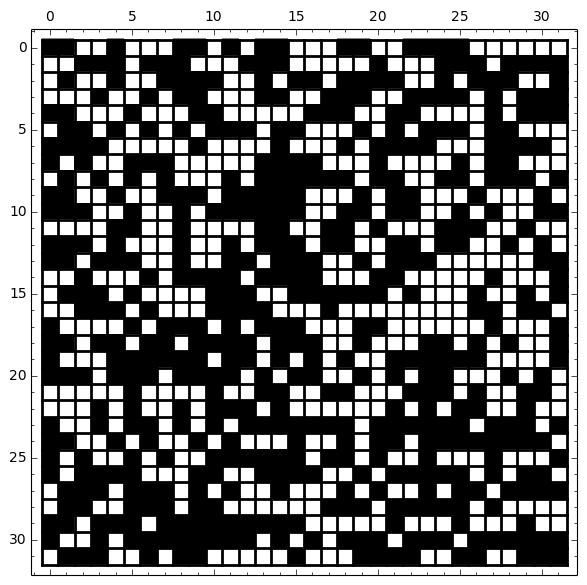
\includegraphics[scale=0.5]{figures/BC_lfsr_ex1.png}   %BERM0
\end{center}
\caption{Visualisierung der pseudozufälligen Bitfolge aus Abbildung~\ref{Sage-code-bool-psr},
   erzeugt mit dem SageMath-Beispiel~\ref{Sage-code-bool-psr}
   (1 = schwarz, 0 = weiß)}\label{fig-bool-lfsr2}
\end{figure}
\clearpage

\subsection{Algebraischer Angriff\index{algebraischer Angriff}\index{Angriff!algebraisch}
            auf lineare Schieberegister}\label{ss-bool-alg2}

Auch einfache Zufallsgeneratoren\index{Zufallsgenerator} wie die linearen
Schieberegister\index{lineares Schieberegister}\index{Schieberegister!linear} liefern,
wie gesehen, Bitfolgen, die mit statistischen Mitteln nicht ohne weiteres
von "`echtem"' Zufall unterschieden werden können und für statistische
Methoden der Kryptoanalyse keinen unmittelbar erfolgversprechenden
Ansatz bieten. Anders sieht es aus, wenn man
bekannten Klartext\index{bekannter Klartext}\index{Klartext!bekannt} annimmt
-- dann erhält man Gleichungen für die Schlüsselbits. Werden die
Schlüsselbits nach einem einfachen Algorithmus erzeugt, kann man
mit algebraischer
Kryptoanalyse\index{algebraische Kryptoanalyse}\index{Kryptoanalyse!algebraisch},
d.\,h. durch Auflösung dieser Gleichungen, auf Erfolg hoffen. Dies ist besonders
für lineare Schieberegister\footnote{%
  Die "`Rückkopplung"' wird in der Bezeichnungsweise meistens weggelassen,
  wenn keine Missverständnisse zu befürchten sind, ist hier aber implizit
  immer mit gemeint.
} der Fall.

Nehmen wir an, ein lineares
Schieberegister\index{lineares Schieberegister}\index{Schieberegister!linear}
hat den Schlüsselbitstrom $u_0, u_1, \ldots$ nach den
Formeln~(\ref{eq-bool-lfsr1}) und (\ref{eq-bool-lfsr2}) erzeugt.
Mit diesem Schlüsselstrom\index{Schlüsselstrom} wurde ein
Klartext $a$ per XOR\index{XOR}\index{Verschlüsselung!XOR}
zum Geheimtext $c$ verschlüsselt, $c_i = a_i + u_i$
für $i = 0, 1, \ldots$ Was kann die Gegnerin erreichen, wenn sie ein
Stück vom Anfang des Klartexts kennt?

Nun, kennt sie die ersten $l+1$ Bits des Klartexts, so hat sie sofort
die entsprechenden Bits $u_0, \ldots, u_l$ des Schlüsselstroms,
insbesondere den Startwert. Für die noch unbekannten Koeffizienten
$s_i$ kennt sie eine lineare Relation:
\[
     s_1 u_{l-1} + \cdots + s_l u_0 = u_l.
\]
Jedes weitere bekannte Bit des Klartexts liefert eine weitere Relation,
und mit $l$ solchen Relationen, also insgesamt $2l$ Bits an bekanntem
Klartext, liefert die sehr einfache Lineare
Algebra\index{lineare Algebra}\index{Algebra!lineare} über dem Körper
$\F_2$ im allgemeinen eine eindeutige Lösung. Die
$l \times l$-Koeffizientenmatrix dieses linearen
Gleichungssystems\index{lineares Gleichungssystem}\index{Gleichungssystem!linear}
ist im Wesentlichen die Matrix $U$ des nächsten Abschnitts. Ein
kleiner Umweg macht die Lösung noch ein wenig eleganter -- in den nächsten,
etwas mehr Mathematik voraussetzenden Abschnitten wird bewiesen:

\begin{satz}\label{thm-bool-lfsr}
  Ein lineares Schieberegister\index{lineares Schieberegister}\index{Schieberegister!linear}
  der Länge $l$ ist aus den ersten $2l$ Bits
  vorhersagbar. Der Aufwand dazu beträgt ungefähr $\frac{1}{3} \cdot l^3$
  Bitoperationen.
\end{satz}

\subsubsection*{Vorhersage linearer Schieberegister}

Nehmen wir an, wir kennen die ersten $2l$ Bits $u_0, \ldots, u_{2l-1}$
aus einem linearen Schieberegister\index{lineares Schieberegister}\index{Schieberegister!linear}
der Länge $l$. Die Lineare Algebra lässt
sich eleganter formulieren, wenn man die {\bf Zustandsvektoren\index{Zustandsvektor}}
\[
     u_{(i)} = (u_i, \ldots, u_{i+l-1}) \quad \text{für } i = 0, 1, \ldots
\]
verwendet. Dabei ist $u_{(i)}$ gerade der Inhalt des Registers beim Schritt
Nummer $i$ (in umgekehrter Reihenfolge) -- d.\,h., die Analyse konzentriert
sich nicht auf den Output, sondern setzt bei den Zuständen an. Die
Rekursionsformel~(\ref{eq-bool-lfsr1}) kann man dann für $n \geq l$ in
Matrixform als
\[
     \begin{pmatrix} u_{n-l+1} \\ \vdots \\ u_{n-1} \\ u_{n} \end{pmatrix}
     =
     \begin{pmatrix} 0      & 1      & \ldots & 0      \\
                     \vdots & \vdots & \ddots & \vdots \\
                     0      & 0      & \ldots & 1      \\
                     s_l    & s_{l-1}    & \ldots & s_1 \end{pmatrix}
     \begin{pmatrix} u_{n-l} \\ \vdots \\ u_{n-2} \\ u_{n-1} \end{pmatrix}
\]
schreiben oder sehr knapp und übersichtlich in der Form (mit substituierten Indizes
$m = n-l+1$)
\[
     u_{(m)} = S \cdot u_{(m-1)} \quad \text{für } m \geq 1\,,
\]
wobei $S$ die Koeffizientenmatrix ist. Noch einen Schritt weiter gehend
fasst man $l$ aufeinanderfolgende Zustandsvektoren
$u_{(i)}, \ldots, u_{(i+l-1)}$ zu einer Zustandsmatrix
\[
     U_{(i)} = \begin{pmatrix} u_i      & u_{i+1}      & \ldots & u_{i+l-1}      \\
                               u_{i+1} & u_{i+2} & \ldots & u_{i+l} \\
                               \vdots  & \vdots & \ddots & \vdots     \\
                     u_{i+l-1}    & u_{i+l} & \ldots & u_{2l-2} \end{pmatrix}
\]
zusammen, setzt $U = U_{(0)}$, $V = U_{(1)}$, und erhält damit die Formel
\[
     V  =  S \cdot U,
\]
die die unbekannten Koeffizienten $s_1, \ldots, s_l$ durch die bekannten
Klartextbits $u_0, \ldots, u_{2l-1}$ ausdrückt. Vor allem aber gestattet sie,
als Lohn für die Bemühungen sofort die Lösung hinzuschreiben -- vorausgesetzt,
die Matrix $U$ ist invertierbar:
\[
     S  =  V \cdot U^{-1},
\]
denn aus der Matrix $S$ kann man ja die Koeffizienten $s_j$ auslesen.
Mehr zur Invertierbarkeit später.

\subsubsection*{Beispiel}

Wir haben einen Geheimtext vorliegen:
\begin{verbatim}
   10011100 10100100 01010110 10100110 01011101 10101110
   01100101 10000000 00111011 10000010 11011001 11010111
   00110010 11111110 01010011 10000010 10101100 00010010
   11000110 01010101 00001011 11010011 01111011 10110000
   10011111 00100100 00001111 01010011 11111101
\end{verbatim}
Wir vermuten, dass er XOR-chiffriert\index{XOR}\index{Verschlüsselung!XOR}
ist mit einem Schlüsselstrom, der
durch ein lineares Schieberegister der Länge $l = 16$ erzeugt wurde.
Der Kontext lässt vermuten, dass der Text mit dem Wort "`Treffpunkt"'
beginnt. Zum Brechen benötigen wir nach der Theorie 32 Bits, also
nur die ersten vier Buchstaben. Daraus ermitteln wir 32 Bits des
Schlüsselstroms:
\begin{verbatim}
    01010100 01110010 01100101 01100110 = T r e f
    10011100 10100100 01010110 10100110   cipher bits
    -------- -------- -------- --------
    11001000 11010110 00110011 11000000   key bits
\end{verbatim}
Im SageMath-Beispiel~\ref{Sage-code-bool-lfsr2} wird die Koeffizientenmatrix
bestimmt. Die letzte Zeile sagt uns, dass die $s_i = 0$ sind außer
$s_{16} = s_5 = s_3 = s_2 = 1$.

Damit kennen wir das Schieberegister und den Startwert, können den
gesamten Schlüsselstrom berechnen -- ja, es ist der aus Abbildung~\ref{Sage-code-bool-psr}
-- und damit den Klartext herstellen
(der übrigens nicht ganz so beginnt wie vermutet).

\begin{sagecode}
\begin{verbatim}

sage: l = 16
sage: kbits =
      [1,1,0,0,1,0,0,0,1,1,0,1,0,1,1,0,0,0,1,1,0,0,1,1,1,1,0,0,0,0,0,0]
sage: ulist = []
sage: for i in range(0,l):
        state = kbits[i:(l+i)]
        ulist.append(state)
sage: U = matrix(GF(2),ulist)
sage: det(U)
1
sage: W = U.inverse()
sage: vlist = []
sage: for i in range(1,l+1):
        state = kbits[i:(l+i)]
        vlist.append(state)
sage: V = matrix(GF(2),vlist)
sage: S = V*W
sage: S
[0 1 0 0 0 0 0 0 0 0 0 0 0 0 0 0]
[0 0 1 0 0 0 0 0 0 0 0 0 0 0 0 0]
[0 0 0 1 0 0 0 0 0 0 0 0 0 0 0 0]
[0 0 0 0 1 0 0 0 0 0 0 0 0 0 0 0]
[0 0 0 0 0 1 0 0 0 0 0 0 0 0 0 0]
[0 0 0 0 0 0 1 0 0 0 0 0 0 0 0 0]
[0 0 0 0 0 0 0 1 0 0 0 0 0 0 0 0]
[0 0 0 0 0 0 0 0 1 0 0 0 0 0 0 0]
[0 0 0 0 0 0 0 0 0 1 0 0 0 0 0 0]
[0 0 0 0 0 0 0 0 0 0 1 0 0 0 0 0]
[0 0 0 0 0 0 0 0 0 0 0 1 0 0 0 0]
[0 0 0 0 0 0 0 0 0 0 0 0 1 0 0 0]
[0 0 0 0 0 0 0 0 0 0 0 0 0 1 0 0]
[0 0 0 0 0 0 0 0 0 0 0 0 0 0 1 0]
[0 0 0 0 0 0 0 0 0 0 0 0 0 0 0 1]
[1 0 0 0 0 0 0 0 0 0 0 1 0 1 1 0]
\end{verbatim}
\caption{Bestimmung einer Koeffizientenmatrix}\label{Sage-code-bool-lfsr2}
\end{sagecode}

\subsubsection*{Beweis des Satzes}

Für den Fall, dass die Zustandsmatrix $U = U_{(0)}$ invertierbar ist,
haben wir oben schon gezeigt, dass die Koeffizienten eindeutig bestimmbar sind.
Insbesondere ist dann das Schieberegister bekannt und aller weitere Output
vorhersagbar. Wir müssen uns also noch mit der Möglichkeit auseinandersetzen,
dass die Matrix $U$ nicht invertierbar sein könnte.

Falls einer der ersten $l$ Zustandsvektoren (= Zeilen der Matrix $U$)
Null ist, sind auch alle weiteren Null, die Vorhersage ist also trivial.

Wir können also annehmen, dass diese Vektoren alle nicht Null, aber linear
abhängig sind. Dann gibt es einen kleinsten Index $k \geq 1$, so dass
$u_{(k)}$ in dem von $u_{(0)}, \ldots, u_{(k-1)}$ aufgespannten
Unterraum liegt. D.\,h., es gibt Koeffizienten $t_1, \ldots, t_k \in \F_2$ mit
\[
     u_{(k)}  =  t_1 u_{(k-1)} + \cdots + t_k u_{(0)}.
\]
Dann gilt aber auch $u_{(k+1)} = S\cdot u_{(k)} =
t_1 S\cdot u_{(k-1)} + \cdots + t_k S\cdot u_{(0)} =
t_1 u_{(k)} + \cdots + t_k u_{(1)}$ und weiter durch Induktion
\[
     u_{(n)}  =  t_1 u_{(n-1)} + \cdots + t_k u_{(n-k)}
     \quad \text{für alle } n \geq k.
\]
Durch diese Formel werden also auch alle weiteren Bits vorhergesagt.

Die Aussage über den Aufwand folgt aus Satz~\ref{thm-bool-lin}.

\begin{description}
   \item[Diskussion:] ~
      \begin{itemize}
         \item Diese Überlegung ergibt für den Fall einer nicht invertierbaren
            Zustandsmatrix ein kürzeres lineares Schieberegisters (der Länge
            $k < l$), das die gleiche Folge erzeugt. In diesem Fall werden
            die Koeffizienten des originalen Registers also nicht bestimmt,
            aber die weitere Folge trotzdem korrekt vorhergesagt.
         \item Wenn nicht die ersten Bits, sondern $2l$ zusammenhängende
            Bits an späterer Stelle bekannt sind, ergibt der Satz zunächst
            nur eine Berechnung der späteren Bits. Im Regelfall, wo die
            Zustandsmatrix $U$ invertierbar ist, ist das Register aber
            dann völlig bekannt und kann natürlich auch rückwärts zur
            Bestimmung der Vorgängerbits eingesetzt werden. Ist die
            Zustandsmatrix nicht invertierbar, kann man das gleiche mit dem
            eben konstruierten kürzeren linearen Schieberegister erreichen.
         \item Etwas komplizierter wird die Situation, wenn man zwar $2l$
            Bits des Schlüsselstroms kennt, diese aber nicht zusammenhängen.
            Auch dann erhält man lineare Relationen, in denen aber
            zusätzlich unbekannte Zwischenbits vorkommen. Ist $m$ die Zahl
            der Lücken, so hat man dann insgesamt $l+m$ lineare Gleichungen
            für $l+m$ unbekannte Bits.
         \item Was aber, wenn auch die Länge $l$ des Registers unbekannt ist?
            Das Durchprobieren aller Werte $l = 1, 2, 3, \ldots$ ist sicher
            lästig, aber machbar. Es gibt aber auch den Algorithmus von
            Berlekamp-Massey\footnote{%
            in SageMath als {\tt sage.crypto.lfsr.berlekamp\_massey} enthalten,
            in CrypTool\,2 unter
            "`Kryptoanalyse"'/"`Generisch"'/"`Berlekamp-Massey-Algorithmus"'
            zu finden
            }, der ohne vorherige Kenntnis
            von $l$ sehr effizient ist. Dessen Behandlung würde aber hier
            zu weit führen.
      \end{itemize}
\end{description}

\subsubsection*{Fazit}

Kryptoanalyse bedeutet für Zufallsgeneratoren\index{Zufallsgenerator} wie in Abbildung~\ref{fig-bool-prg},
aus einem Teil ihres Outputs eine der folgenden Informationen zu bestimmen:
\begin{itemize}
\item die geheimen Parameter,
\item den Startwert,
\item weitere Teile des Outputs ("`Vorhersageproblem\index{Vorhersageproblem}"').
\end{itemize}
Wie wir bei den linearen
Schieberegistern\index{lineares Schieberegister}\index{Schieberegister!linear}
gesehen haben, ist es
realistisch, das Vorhersageproblem anzugehen, das auch lösbar sein
kann, wenn die Bestimmung der internen Parameter nicht gelingt.
Wir halten fest:
\begin{quote}
   {\em Die Kryptoanalyse eines Zufallsgenerators bedeutet in erster Linie
   die Lösung des Vorhersageproblems. Ein Zufallsgenerator\index{Zufallsgenerator}
   ist kryptographisch
   sicher, wenn sein Vorhersageproblem nicht effizient lösbar ist.}
\end{quote}

\begin{quote}
   {\em Lineare Schieberegister\index{lineares Schieberegister}\index{Schieberegister!linear}
   sind kryptographisch nicht sicher.}
\end{quote}

\subsection{Nichtlinearität\index{Nichtlinearität} für Schieberegister
   -- Ansätze}\label{ss-bool-nlsr}

Lineare Schieberegister sind beliebt -- vor allem bei Elektro-Ingenieuren
und beim Militär -- denn sie sind
\begin{itemize}
	\item sehr einfach zu realisieren,
	\item extrem effizient in Hardware,
	\item als Zufallsgeneratoren für statistische Zwecke sehr gut geeignet,
	\item problemlos in gro"ser Anzahl parallel zu betreiben,
	\item aber leider kryptologisch völlig unsicher.
\end{itemize}
Um die positiven Eigenschaften zu nutzen und die kryptologische Schwäche
zu vermeiden, gibt es verschiedene Ansätze.

\subsubsection*{Ansatz 1: Nichtlineare Rückkopplung}

Die nichtlineare Rückkopplung\index{Rückkopplung}
folgt dem Schema aus Abbildung~\ref{fig-bool-fsr}
mit einer nichtlinearen Booleschen Funktion\index{Boolesche
Funktion}\index{Funktion!Boolesche} $f$.
Sie wird hier nicht weiter behandelt; ein ganz
einfaches, kryptographisch ungeeignetes Beispiel war das
SageMath-Beispiel~\ref{Sage-code-bool-fsr1}. Man kann aber auch
allgemein zeigen, dass solche nichtlinearen Schieberegister
(nonlinear feedback, NLFSR\footnote{%
   für Non-Linear Feedback Shift Register\index{Schieberegister!nichtlinear}
}
), für sich allein genommen, unter realistischen Annahmen
im praktischen Einsatz nicht kryptographisch
sicher sind \cite{Pom2016}.


\subsubsection*{Ansatz 2: Nichtlinearer Ausgabefilter}

Der nichtlineare Ausgabefilter\index{Ausgabefilter}
(Non-Linear Feedforward) folgt dem Schema
aus Abbildung~\ref{fig-bool-nlf}.
Das Schieberegister selbst ist linear. Der nichtlineare Ausgabefilter
ist ein Spezialfall des nächsten Ansatzes.

\begin{figure}
\begin{center}
\begin{picture}(320,150)
  \linethickness{2pt}
  \put(20,20){\line(1,0){260}}
  \put(20,20){\line(0,1){30}}
  \put(20,50){\line(1,0){260}}
  \put(280,20){\line(0,1){30}}
  \put(260,120){\circle{30}}
  \put(256,117){$f$}

  \linethickness{1pt}
  \put(60,20){\line(0,1){30}}
  \put(100,20){\line(0,1){30}}
  \put(240,20){\line(0,1){30}}
  \put(200,20){\line(0,1){30}}
  \put(110,30){\ldots}
  \put(180,30){\ldots}

  \put(40,20){\line(0,-1){20}}
  \put(80,20){\line(0,-1){20}}
  \put(220,20){\line(0,-1){20}}
  \put(260,20){\line(0,-1){20}}
  \put(260,0){\line(-1,0){260}}
  \put(0,0){\line(0,1){35}}
  \put(0,35){\vector(1,0){20}}

  \put(260,50){\vector(0,1){53}}
  \put(220,50){\vector(1,2){29}}
  \put(80,50){\line(0,1){25}}
  \put(80,75){\vector(4,1){163}}
  \put(40,50){\line(0,1){70}}
  \put(40,120){\vector(1,0){203}}

  \put(277,120){\vector(1,0){43}}
\end{picture}
\end{center}
\caption{Nichtlinearer Ausgabefilter für ein lineares Schieberegister}\label{fig-bool-nlf}
\end{figure}

\subsubsection*{Ansatz 3: Nichtlinearer Kombinierer\index{Kombinierer}}

Hier wird eine "`Batterie"' aus $n$ linearen Schieberegistern -- die durchaus
unterschiedliche Länge haben können und sollen -- parallel betrieben.
Ihre Outputfolgen werden in eine
Boolesche Funktion\index{Boolesche Funktion}\index{Funktion!Boolesche}
$f\!\!: \F_2^n \longrightarrow \F_2$ gefüttert\footnote{%
   daher auch hierfür gelegentlich die Bezeichnung Non-Linear Feedforward
}, siehe Abbildung~\ref{fig-bool-nlc}.
Ein Ansatz zur Analyse dieses Verfahrens folgt in Abschnitt~\ref{ss-bool-bsana}.

\begin{figure}
\begin{center}
\begin{picture}(350,200)
  \linethickness{2pt}
  \put(20,20){\line(1,0){260}}
  \put(20,20){\line(0,1){30}}
  \put(20,50){\line(1,0){260}}
  \put(280,20){\line(0,1){30}}

  \linethickness{1pt}
  \put(60,20){\line(0,1){30}}
  \put(100,20){\line(0,1){30}}
  \put(240,20){\line(0,1){30}}
  \put(200,20){\line(0,1){30}}
  \put(110,30){\ldots}
  \put(180,30){\ldots}

  \put(40,20){\line(0,-1){20}}
  \put(80,20){\line(0,-1){20}}
  \put(220,20){\line(0,-1){20}}
  \put(260,20){\line(0,-1){20}}
  \put(260,0){\line(-1,0){260}}
  \put(0,0){\line(0,1){35}}
  \put(0,35){\vector(1,0){20}}

  \linethickness{2pt}
  \put(20,150){\line(1,0){260}}
  \put(20,150){\line(0,1){30}}
  \put(20,180){\line(1,0){260}}
  \put(280,150){\line(0,1){30}}

  \linethickness{1pt}
  \put(60,150){\line(0,1){30}}
  \put(100,150){\line(0,1){30}}
  \put(240,150){\line(0,1){30}}
  \put(200,150){\line(0,1){30}}
  \put(110,160){\ldots}
  \put(180,160){\ldots}

  \put(40,150){\line(0,-1){20}}
  \put(80,150){\line(0,-1){20}}
  \put(220,150){\line(0,-1){20}}
  \put(260,150){\line(0,-1){20}}
  \put(260,130){\line(-1,0){260}}
  \put(0,130){\line(0,1){35}}
  \put(0,165){\vector(1,0){20}}

  \put(80,100){$\vdots$}
  \put(220,100){$\vdots$}
  \put(80,70){$\vdots$}
  \put(220,70){$\vdots$}

  \put(280,165){\vector(1,0){20}}
  \put(280,35){\vector(1,0){20}}
  \put(315,100){\oval(30,160)}
  \put(330,100){\vector(1,0){20}}
  \put(313,97){$f$}
\end{picture}
\end{center}
\caption{Nichtlinearer Kombinierer}\label{fig-bool-nlc}
\end{figure}

\subsubsection*{Ansatz 4: Auswahlsteuerung/Dezimierung/Taktung}

Weitere Möglichkeiten bestehen in verschiedenen Methoden zur Steuerung
einer Batterie von $n$ parallel betriebenen linearen Schieberegistern
durch ein weiteres lineares Schieberegister:
\begin{itemize}
	\item Bei der {\bf Auswahlsteuerung}\index{Auswahlsteuerung}
        wird je nach Zustand des "`Hilfsregisters"'
	   das aktuelle Output-Bit von genau einem der "`Batterie-Register"' als
	   Output des Zufallsgenerators ausgewählt. Allgemeiner kann man auch
	   eine Auswahl "`$r$ aus $n$"' treffen.
	\item Bei der {\bf Dezimierung}\index{Dezimierung} nimmt man
        im allgemeinen $n = 1$ an und gibt das
	   Output-Bit des einen Batterie-Registers nur dann aus, wenn das
	   Hilfsregister einen bestimmten Zustand hat. Diese Art der Dezimierung
	   kann man natürlich analog auf jede Bitfolge anwenden.
	\item Bei der {\bf Taktung}\index{Taktung} gibt der Zustand
        des Hilfsregisters an, welche
	   der Batterie-Register im aktuellen Taktzyklus weitergeschoben werden
	   (und um wie viele Positionen) und welche in ihrem momentanen Zustand bleiben.
	   Das ist vergleichbar mit der Steuerlogik von
        Rotor-Maschinen\index{Rotor-Maschine}.
\end{itemize}
Diese Ansätze lassen sich oft bequem auch als nichtlineare Kombinierer schreiben,
so dass Ansatz 3 als der gängigste Ansatz zur Rettung der linearen
Schieberegister\index{lineares Schieberegister}\index{Schieberegister!linear}
angesehen werden kann.

Der Mobilfunk-Verschlüsselungsstandard
\href{http://de.wikipedia.org/wiki/A5\_(Algorithmus)}{A5/1}\index{A5}  %% Ok in PDF, aber 1. in href muss man "_" maskieren, was unschön ist. 2. Wie sichtbar machen, dass hinter "A5/1" eine URL, auf die man tippen kann und die einen Balloontext hat. Ich habe urlcolor=cyan gesetzt. Gibt es etwas Eleganteres und etwas, was man im s/w-Ausdruck besser sieht (black und blue sieht man gut)? ==> Todo Doris
% yyy \href{\url{http://de.wikipedia.org/wiki/A5_(Algorithmus)}}{A5/1}\index{A5}  %% lässt sich nicht compilieren
% yyy \url{http://de.wikipedia.org/wiki/A5_(Algorithmus)}{A5/1}\index{A5}  %% Gibt URL aus
verwendet drei leicht unterschiedlich getaktete lineare Schieberegister
der Längen 19, 22 und 23 mit jeweils maximaler Periode, deren
Outputströme linear (nämlich einfach durch binäre Addition)
kombiniert werden. Bei A5/2 -- das noch schwächer ist -- wird
die Taktung durch ein Hilfsregister geregelt. Beide Varianten
lassen sich auf handelsüblichen PCs in Echtzeit brechen.

Der Bluetooth-Verschlüsselungsstandard $\mathrm{E}_0$\index{E0} verwendet vier
lineare Schieberegister, die nichtlinear kombiniert werden. Dieses Verfahren
ist etwas stärker als A5, aber auch zu schwach für echte Sicherheit \cite{Schm2016}.

\subsubsection*{Beispiel: Der Geffe-Generator}

Das einfachste Beispiel für die Auswahlsteuerung ist der
Geffe-Generator\index{Geffe-Generator},
der durch das Schema in Abbildung~\ref{fig-bool-gef}
beschrieben wird. Die Ausgabe ist $x$, wenn $z = 0$, und $y$, wenn
$z = 1$. Das kann man so als Formel ausdrücken:
\begin{eqnarray*}
   u & = & \begin{cases}
              x, & \text{wenn } z = 0, \\
              y, & \text{wenn } z = 1
           \end{cases} \\
      & = & (1 - z) x + zy = x + zx + zy.
\end{eqnarray*}
Also lässt sich der Geffe-Generator auch durch einen nichtlinearen
Kombinierer mit einer Booleschen Funktion
$f\!\!: \F_2^3 \longrightarrow \F_2$ vom Grad 2 beschreiben. Diese
wird zur späteren Verwendung im SageMath-Beispiel~\ref{Sage-code-bool-gef}
erzeugt.

\begin{figure}
\begin{center}
\setlength{\unitlength}{1pt}
\begin{picture}(350,200)
  \linethickness{2pt}
  \put(20,20){\line(1,0){260}}
  \put(20,20){\line(0,1){30}}
  \put(20,50){\line(1,0){260}}
  \put(280,20){\line(0,1){30}}

  \linethickness{1pt}
  \put(60,20){\line(0,1){30}}
  \put(100,20){\line(0,1){30}}
  \put(240,20){\line(0,1){30}}
  \put(200,20){\line(0,1){30}}
  \put(110,30){\ldots}
  \put(180,30){\ldots}

  \put(40,20){\line(0,-1){20}}
  \put(80,20){\line(0,-1){20}}
  \put(220,20){\line(0,-1){20}}
  \put(260,20){\line(0,-1){20}}
  \put(260,0){\line(-1,0){260}}
  \put(0,0){\line(0,1){35}}
  \put(0,35){\vector(1,0){20}}

  \linethickness{2pt}
  \put(20,80){\line(1,0){260}}
  \put(20,80){\line(0,1){30}}
  \put(20,110){\line(1,0){260}}
  \put(280,80){\line(0,1){30}}

  \linethickness{1pt}
  \put(60,80){\line(0,1){30}}
  \put(100,80){\line(0,1){30}}
  \put(240,80){\line(0,1){30}}
  \put(200,80){\line(0,1){30}}
  \put(110,90){\ldots}
  \put(180,90){\ldots}

  \put(40,80){\line(0,-1){20}}
  \put(80,80){\line(0,-1){20}}
  \put(220,80){\line(0,-1){20}}
  \put(260,80){\line(0,-1){20}}
  \put(260,60){\line(-1,0){260}}
  \put(0,60){\line(0,1){35}}
  \put(0,95){\vector(1,0){20}}

  \linethickness{2pt}
  \put(50,160){\line(1,0){260}}
  \put(50,160){\line(0,1){30}}
  \put(50,190){\line(1,0){260}}
  \put(310,160){\line(0,1){30}}

  \linethickness{1pt}
  \put(90,160){\line(0,1){30}}
  \put(130,160){\line(0,1){30}}
  \put(270,160){\line(0,1){30}}
  \put(230,160){\line(0,1){30}}
  \put(140,170){\ldots}
  \put(210,170){\ldots}

  \put(70,160){\line(0,-1){20}}
  \put(110,160){\line(0,-1){20}}
  \put(250,160){\line(0,-1){20}}
  \put(290,160){\line(0,-1){20}}
  \put(290,140){\line(-1,0){260}}
  \put(30,140){\line(0,1){35}}
  \put(30,175){\vector(1,0){20}}

  \put(310,175){\line(1,0){20}}
  \put(330,175){\line(0,-1){40}}
  \put(333,152){$z$}
  \put(330,135){\line(-1,0){15}}
  \put(315,135){\vector(0,-1){25}}

  \put(280,95){\vector(1,0){20}}
  \put(288,97){$x$}
  \put(280,35){\vector(1,0){20}}
  \put(288,38){$y$}
  \put(315,65){\oval(30,90)}
  \put(330,65){\line(-1,-1){30}}
  \put(330,65){\vector(1,0){20}}
\end{picture}
\end{center}
\caption{Geffe-Generator}\label{fig-bool-gef}
\end{figure}

\begin{sagecode}
\begin{verbatim}

sage: geff = BoolF(str2bbl("00011100"),method="ANF")
sage: geff.printTT()
Value at 000 is 0
Value at 001 is 0
Value at 010 is 0
Value at 011 is 1
Value at 100 is 1
Value at 101 is 0
Value at 110 is 1
Value at 111 is 1
\end{verbatim}
\caption{Die Geffe-Funktion}\label{Sage-code-bool-gef}
\end{sagecode}

\subsection{Implementation eines nichtlinearen Kombinierers}\label{ss-bool-ncsr}

Ein nichtlinearer Kombinierer\index{Kombinierer} benötigt mehrere parallel betriebene
lineare Schieberegister. Dies legt nahe, diese als Objekte zu
implementieren, d.\,h., eine Klasse {\tt LFSR} zu definieren\footnote{%
   siehe auch in CrypTool\,2 unter "`Protokolle"'/"`LFSR"' bzw. "`NLFSR"'
}.

\begin{description}
   \item[Klasse {\tt LSFR}:] ~
      \begin{description}
         \item[Attribute:] ~
            \begin{itemize}
               \item {\tt length}: die Länge des Registers
               \item {\tt taplist}: die Liste der Koeffizienten ("`Taps"'\footnote{%
                    auf deutsch etwa "`Abzweig"' oder "`Abgriff"', weil bei einer
                    Hardware-Implementierung genau an diesen Stellen die für die
                    Rückkopplung verwendeten Bits abgegriffen werden
                  }), die die  rückzukoppelnden Bits definieren (konstant)
               \item {\tt state}: der Zustand des Registers (veränderbar)
            \end{itemize}
         \item[Methoden:] ~
            \begin{itemize}
               \item {\tt setLength}: Definition der Länge (nur implizit bei
                  der Initialisierung verwendet)
               \item {\tt setTaps}: Besetzung der Tap- (= Koeffizienten-) Liste
                  (nur implizit bei der Initialisierung verwendet)
               \item {\tt setState}: Belegung des Registers mit einem Zustand
               \item {\tt getLength}: Ausgabe der Länge
               \item {\tt nextBits}: Erzeugung einer vorgegebenen Anzahl von
                  Ausgabebits und kontinuierliche Weiterschaltung des Zustands
            \end{itemize}
      \end{description}
\end{description}
Dazu ist es zur Überwachung des Registers praktisch, noch eine Methode
(die in Python\index{Python} generisch {\tt \_\_str\_\_} heißt) zu haben, die die
Attribute in lesbarer Form ausgibt.

Für die Implementation siehe das SageMath-Beispiel~\ref{Sage-code-bool-lfsr3}
im Abschnitt~\ref{ss-bool-lfsrclass}.

\subsubsection*{Beispiel: Geffe-Generator\index{Geffe-Generator}}

Zunächst wählen wir drei lineare Schieberegister der Längen 15, 16 und 17,
deren Perioden\footnote{%
  nach den Listen primitiver Polynome in \cite{Menezes2001}
} $2^{15} - 1 = 32767$, $2^{16} - 1 = 65535$ und
$2^{17} - 1 = 131071$ sind, und diese sind paarweise teilerfremd, siehe
SageMath-Beispiel~\ref{Sage-code-bool-per}.
Fasst man ihren Output in jedem Takt zu Bitblöcken der Länge $3$
zusammen, so hat diese Folge eine Periode der eindrucksvollen Länge
$281459944554495$, also knapp $300 \times 10^{12}$ (300 Billionen\footnote{%
  europäische Billionen. Amerikanisch wären das 300 Trillionen.
}).
Die drei Register werden im SageMath-Beispiel~\ref{Sage-code-bool-regs}
definiert; die Rekursionsformel für das dritte davon, das
Steuerungsregister {\tt reg17}, ist z.\,B. $u_n = u_{n-3} + u_{n-17}$,
da genau die Taps 3 und 17 gesetzt sind.
Mit jedem von ihnen wird eine Folge der Länge 100 erzeugt,
siehe SageMath-Beispiel~\ref{Sage-code-bool-seqs}. Diese werden im
SageMath-Beispiel~\ref{Sage-code-bool-gef-seq} mithilfe der
Geffe-Funktion kombiniert.

\begin{sagecode}
\begin{verbatim}

sage: n15 = 2**15 - 1; n15
32767
sage: n15.factor()
7 * 31 * 151
sage: n16 = 2**16 - 1; n16
65535
sage: n16.factor()
3 * 5 * 17 * 257
sage: n17 = 2**17 - 1; n17
131071
sage: n17.factor()
131071
sage: period = n15 * n16 * n17; period
281459944554495
\end{verbatim}
\caption{Eine Periodenberechnung}\label{Sage-code-bool-per}
\end{sagecode}

\begin{sagecode}
\begin{verbatim}

sage: reg15 = LFSR([1,0,0,0,0,0,0,0,0,0,0,0,0,0,1])
sage: reg15.setState([0,1,1,0,1,0,1,1,0,0,0,1,0,0,1])
sage: print(reg15)
Length: 15 | Taps: 100000000000001 | State: 011010110001001
sage: reg16 = LFSR([0,1,1,0,1,0,0,0,0,0,0,0,0,0,0,1])
sage: reg16.setState([0,1,1,0,1,0,1,1,0,0,0,1,0,0,1,1])
sage: print(reg16)
Length: 16 | Taps: 0110100000000001 | State: 0110101100010011
sage: reg17 = LFSR([0,0,1,0,0,0,0,0,0,0,0,0,0,0,0,0,1])
sage: reg17.setState([0,1,1,0,1,0,1,1,0,0,0,1,0,0,1,1,1])
sage: print(reg17)
Length: 17 | Taps: 00100000000000001 | State: 01101011000100111
\end{verbatim}
\caption{Drei lineare Schieberegister}\label{Sage-code-bool-regs}
\end{sagecode}

\begin{sagecode}
\begin{verbatim}

sage: nofBits = 100
sage: outlist15 = reg15.nextBits(nofBits)
sage: print(outlist15)
[1, 0, 0, 1, 0, 0, 0, 1, 1, 0, 1, 0, 1, 1, 0, 1, 1, 1, 0, 0,
 0, 0, 1, 0, 0, 1, 1, 0, 1, 1, 0, 1, 0, 0, 0, 0, 0, 1, 1, 1,
 0, 1, 1, 0, 1, 1, 0, 0, 0, 0, 0, 0, 1, 0, 1, 1, 0, 1, 1, 0,
 1, 1, 1, 1, 1, 1, 1, 0, 0, 1, 0, 0, 1, 0, 0, 1, 0, 1, 0, 1,
 0, 1, 1, 1, 0, 0, 0, 1, 1, 1, 0, 0, 1, 1, 0, 0, 1, 0, 1, 1]
sage: outlist16 = reg16.nextBits(nofBits)
sage: print(outlist16)
[1, 1, 0, 0, 1, 0, 0, 0, 1, 1, 0, 1, 0, 1, 1, 0, 0, 0, 1, 1,
 0, 0, 1, 1, 1, 1, 0, 0, 0, 0, 0, 0, 0, 0, 1, 1, 1, 0, 1, 1,
 1, 0, 0, 0, 1, 1, 1, 0, 0, 0, 0, 0, 1, 0, 0, 0, 1, 1, 1, 0,
 1, 1, 1, 1, 0, 1, 0, 0, 1, 0, 0, 1, 1, 1, 1, 0, 0, 1, 0, 1,
 1, 0, 1, 1, 1, 1, 0, 0, 1, 0, 1, 1, 1, 0, 0, 1, 0, 0, 0, 1]
sage: outlist17 = reg17.nextBits(nofBits)
sage: print(outlist17)
[1, 1, 1, 0, 0, 1, 0, 0, 0, 1, 1, 0, 1, 0, 1, 1, 0, 0, 0, 1,
 0, 0, 0, 0, 0, 0, 1, 1, 0, 0, 1, 1, 1, 1, 1, 1, 0, 1, 1, 0,
 1, 1, 0, 0, 0, 0, 0, 1, 1, 1, 0, 0, 0, 0, 1, 1, 0, 0, 0, 0,
 0, 0, 0, 0, 1, 1, 1, 1, 1, 1, 1, 0, 0, 1, 0, 0, 1, 0, 0, 1,
 0, 1, 0, 1, 0, 1, 0, 1, 1, 0, 0, 1, 0, 1, 1, 0, 0, 1, 1, 0]
\end{verbatim}
\caption{Drei LFSR-Folgen}\label{Sage-code-bool-seqs}
\end{sagecode}
\clearpage

\begin{sagecode}
\begin{verbatim}

sage: outlist = []
sage: for i in range(0,nofBits):
....:     x = [outlist15[i],outlist16[i],outlist17[i]]
....:     outlist.append(geff.valueAt(x))
....:
sage: print(outlist)
[1, 1, 0, 1, 0, 0, 0, 1, 1, 1, 0, 0, 0, 1, 1, 0, 1, 1, 0, 1,
 0, 0, 1, 0, 0, 1, 0, 0, 1, 1, 0, 0, 0, 0, 1, 1, 0, 0, 1, 1,
 1, 0, 1, 0, 1, 1, 0, 0, 0, 0, 0, 0, 1, 0, 0, 0, 0, 1, 1, 0,
 1, 1, 1, 1, 0, 1, 0, 0, 1, 0, 0, 0, 1, 1, 0, 1, 0, 1, 0, 1,
 0, 0, 1, 1, 0, 1, 0, 0, 1, 1, 0, 1, 1, 0, 0, 0, 1, 0, 0, 1]
\end{verbatim}
\caption{Die kombinierte Folge}\label{Sage-code-bool-gef-seq}
\end{sagecode}

\subsection{Korrelationsattacken\index{Korrelationsattacke}
    -- die Achillesferse der Kombinierer}\label{ss-bool-bsana}

Sei $f\!\!: \F_2^n \longrightarrow \F_2$ die Kombinierfunktion eines
nichtlinearen Kombinierers\index{Kombinierer}. Die Anzahl
\[
   K_f := \#\{ x = (x_1, \ldots, x_n) \in \F_2^n \:|\: f(x) = x_1 \}
\]
gibt an, wie oft der Funktionswert mit dem ersten Argument übereinstimmt.
Ist sie $> 2^{n-1}$, so ist die Wahrscheinlichkeit für diese Übereinstimmung,
\[
   p = \frac{1}{2^n} \cdot K_f > \frac{1}{2},
\]
also überdurchschnittlich. Die kombinierte Outputfolge "`korreliert"' also
stärker mit dem Output des ersten linearen Schieberegisters, als zufällig
zu erwarten wäre. Ist $p < \frac{1}{2}$, so weicht die Korrelation nach
unten vom zufälligen Wert ab.

Diesen Effekt kann sich die Kryptoanalytikerin bei einem Angriff mit
bekanntem Klartext\index{bekannter Klartext}\index{Klartext!bekannt}
zunutze machen. Angenommen wird, dass ihr die
"`Hardware"', also die Rekursionsformeln für die Register (die Taps) und
auch die Kombinierfunktion $f$, bekannt ist. Gesucht sind die als Schlüssel
betrachteten Startvektoren aller Register. Die Bits $k_0, \ldots, k_{r-1}$
des Schlüsselstroms\footnote{%
  Der Einfachheit der Darstellung halber die ersten $r$ -- für irgendwelche $r$
  bekannten Schlüsselbits funktioniert die Argumentation genauso.
} seien bekannt. Mit einer Exhaustion über die $2^{l_1}$
Startvektoren des ersten Registers erzeugt man jedesmal die Folge
$u_0, \ldots, u_{r-1}$ und zählt die Übereinstimmungen. Zu erwarten ist
\[
   \frac{1}{r}\cdot \#\{i \:|\: u_i = k_i\} \approx
   \begin{cases}
      p & \text{beim richtigen Startvektor,} \\
      \frac{1}{2} & \text{sonst.}
   \end{cases}
\]
Falls $r$ groß genug ist, kann man also den echten Startvektor des ersten
Registers mit einem Aufwand $\sim 2^{l_1}$ (mit hoher Wahrscheinlichkeit)
bestimmen. Macht man dann mit
den anderen Registern genauso weiter, gelingt die Identifikation des
gesamten Schlüssels mit einem Aufwand $\sim 2^{l_1} + \cdots + 2^{l_n}$.
Das ist zwar exponenziell, aber wesentlich geringer als der Aufwand
$\sim 2^{l_1} \cdots 2^{l_n}$ für die naive vollständige Schlüsselsuche.

In der Sprache der linearen
Kryptoanalyse\index{lineare Kryptoanalyse}\index{Kryptoanalyse!linear}
aus \ref{ss-bool-lka} haben
wir hier die lineare Relation\index{lineare Relation}\index{Relation!linear}
\[
     f(x_1, \ldots, x_n) \stackrel{p}{\approx} x_1
\]
für $f$ ausgenutzt. Klar ist, dass man analog jede lineare
Relation ausnutzen kann, um die Komplexität der vollständigen Schlüsselsuche
zu reduzieren\footnote{%
  Eine genauere Analyse der Situation führt auf den Begriff der
  Korrelationsimmunität\index{Korrelationsimmunität}, die mit dem linearen
  Potenzial\index{lineares Potenzial}\index{Potenzial!linear}
  verwandt ist.
}.

\subsubsection*{Korrelationen des Geffe-Generators}

Für den Geffe-Generator\index{Geffe-Generator} kann man die Korrelationen aus
der Wahrheitstafel, Tabelle~\ref{tab-bool-gef-wt}, ablesen:
Als Wahrscheinlichkeit für die Übereinstimmung erhält man also
\[
   p = \begin{cases}
          \frac{3}{4} & \text{für das Register 1 ($x$),} \\
          \frac{3}{4} & \text{für das Register 2 ($y$),} \\
          \frac{1}{2} & \text{für das Register 3 ($z =$ Steuerung).}
       \end{cases}
\]
Daher lassen sich bei einer Korrelationsattacke die Startwerte für die
Register 1 und 2 -- die Batterieregister -- leicht schon aus kurzen
Outputfolgen bestimmen; den Startwert für Register 3, das Steuerungsregister,
findet man dann auch leicht durch Exhaustion.

\begin{table}
\begin{center}
  \begin{tabular}{|c|cccc|cccc|}\hline
      $x$    & $0$ & $0$ & $0$ & $0$ & $1$ & $1$ & $1$ & $1$ \\
      $y$    & $0$ & $0$ & $1$ & $1$ & $0$ & $0$ & $1$ & $1$ \\
      $z$    & $0$ & $1$ & $0$ & $1$ & $0$ & $1$ & $0$ & $1$ \\
    \hline
  $f(x,y,z)$ & $0$ & $0$ & $0$ & $1$ & $1$ & $0$ & $1$ & $1$ \\
    \hline
  \end{tabular}
\end{center}
\caption{Wahrheitstafel der Geffe-Funktion (waagerecht angeordnet)}\label{tab-bool-gef-wt}
\end{table}

Diese Schwachstelle des Geffe-Generators wird im
SageMath-Beispiel~\ref{Sage-code-bool-gef-lp} nachvollzogen, das als
Fortsetzung des SageMath-Beispiels~\ref{Sage-code-bool-gef} einzugeben ist.
Da wir das lineare Profil nur in der Klasse {\tt BoolMap} definiert
haben, müssen wir zuerst die Funktion {\tt geff} als Boolesche
Abbildung interpretieren -- also als Liste der Länge 1 von Booleschen
Funktionen. Das lineare Profil wird als Matrix
mit 2 Spalten und 8 Zeilen gedacht. Die erste Spalte
{\tt [64, 0, 0, 0, 0, 0, 0, 0]} misst die Übereinstimmung mit der
Linearform 0 des Bildbereichs. Sie enthält also keine nennenswerte
Information, außer dass alles durch $64$ zu dividieren ist. Die
zweite Spalte {\tt [0, 0, 16, 16, 16, 16, 0, 0]} wird
(nach dieser Division) in der Tabelle~\ref{tab-bool-gef-korr}
als Liste der Korrelationswahrscheinlichkeiten $p$ interpretiert.
Dabei wird die Formel
\[
     p = \frac{1}{2} \cdot (\pm \sqrt{\lambda} + 1)
\]
verwendet. Ist $\lambda = 0$, so $p = 1/2$. Ist  $\lambda = 1/4$,
so $p = 1/4$ oder $3/4$. Die Entscheidung zwischen diesen beiden
Werten für $p$ kann man anhand der Tabelle~\ref{tab-bool-gef-wt}
treffen.

\begin{table}
\begin{center}
\begin{tabular}{|l|cccccccc|} \hline
  Linearform     & $0$   &   $z$   &   $y$    &   $y+z$   &  $x$    &   $x+z$   &  $x+y$  & $x+y+z$ \\
  Repräsentation & $000$ & $001$ & $010$ & $011$ & $100$ & $101$ & $110$ & $111$ \\ \hline
  Potenzial      & $0$   & $0$   & $1/4$ & $1/4$ & $1/4$ & $1/4$ & $0$   & $0$ \\
  Wahrsch. $p$   & $1/2$ & $1/2$ & $3/4$ & $1/4$ & $3/4$ & $3/4$ & $1/2$ & $1/2$ \\ \hline
\end{tabular}
\end{center}
\caption{Korrelationswahrscheinlichkeiten der Geffe-Funktion}\label{tab-bool-gef-korr}
\end{table}

\begin{sagecode}
\begin{verbatim}

sage: g = BoolMap([geff])
sage: linProf = g.linProf(); linProf
[[64, 0], [0, 0], [0, 16], [0, 16], [0, 16], [0, 16], [0, 0], [0, 0]]
\end{verbatim}
\caption{Lineares Profil der Geffe-Funktion}\label{Sage-code-bool-gef-lp}
\end{sagecode}

Im SageMath-Beispiel~\ref{Sage-code-bool-gef-coi} wird diese Erkenntnis auf
die mit dem Geffe-Generator erzeugte Folge der Länge $100$ angewendet.
Zur Zählung der Koinzidenzen (= Übereinstimmungen) wird die Funktion {\tt coinc} aus dem
SageMath-Beispiel~\ref{Sage-code-bool-div-bbl} (im Anhang) verwendet. Mit dem ersten
Register gibt es $73$, mit dem zweiten $76$ Koinzidenzen, mit dem
dritten dagegen nur $41$. Das passt sehr gut zu den im Rahmen statistischer Schwankungen
theoretisch erwarteten Werten $75$, $75$, $50$.

\begin{sagecode}
\begin{verbatim}

sage: coinc(outlist15,outlist)
73
sage: coinc(outlist16,outlist)
76
sage: coinc(outlist17,outlist)
41
\end{verbatim}
\caption{Koinzidenzen des Geffe-Generators}\label{Sage-code-bool-gef-coi}
\end{sagecode}

\subsubsection*{Analyse des Geffe-Generators\index{Geffe-Generator}}

Diese deutlichen Ergebnisse legen nahe, dass die Analyse der beispielhaft
erzeugten Folge leicht sein sollte. Für eine grobe Erfolgsabschätzung
kann man auf mathematische Strenge verzichten.

Betrachtet wird ein fest vorgegebener Bitblock $b \in \F_2^r$. Wir fragen
zunächst, wie groß die Wahrscheinlichkeit für einen zufälligen Bitblock
$u \in \F_2^r$ ist, an genau $t$ Stellen mit $b$ übereinzustimmen,
also $t$ Koinzidenzen zu haben. Das ist genau die Fragestellung der
symmetrischen Binomialverteilung\index{Binomialverteilung}
(also mit $p = \frac{1}{2}$ als
Wahrscheinlichkeit einer einzelnen Übereinstimmung): Die
Wahrscheinlichkeit für genau $t$ Koinzidenzen ist
\[
     B_{r,\frac{1}{2}}(t)  =  \frac{\binom{r}{t}}{2^r}.
\]
Die Wahrscheinlichkeit für bis zu $T$ Koinzidenzen ist also
\[
     \sum_{t=0}^T B_{r,\frac{1}{2}}(t)
       =  \frac{1}{2^r} \cdot \sum_{t=0}^T \binom{r}{t}.
\]
Wenn $r$ nicht zu groß ist, kann man diesen Wert für eine konkrete
Schranke $T$ explizit ausrechnen. Wenn $r$ nicht zu klein ist,
approximiert man ihn mithilfe der Normalverteilung\index{Normalverteilung}.
Dazu benötigt man den Erwartungswert für die
Anzahl der Koinzidenzen, der $r/2$ ist, die Varianz $r/4$ und die
Standardabweichung $\sqrt{r}/2$.

Wie auch immer man das macht, im Fall $r = 100$ ist (exemplarisch) die
Wahrscheinlichkeit, maximal $65$ Koinzidenzen zu finden, ziemlich
genau $0,999$, die Überschreitungswahrscheinlichkeit also
%%%  Da \textperthousand nicht funktionierte (auch nicht mit package textcomp), \permil genommen.
1\,\permil. Die Exhaustion der Startwerte des Registers 1
umfasst $2^{15} = 32786$ Möglichkeiten (den eigentlich ausgeschlossenen
Startwert $0 \in \F_2^{15}$ zählen wir großzügig mit). Dabei
können wir also etwa $33$ "`Grenzüberschreitungen"' mit mindestens
66 Koinzidenzen erwarten. Darunter sollte der wahre Startwert
von Register 1 sein,
der etwa $75$ Koinzidenzen produzieren sollte und sich vielleicht
sogar durch das Maximum der Koinzidenzen verrät.

Das SageMath-Beispiel~\ref{Sage-code-bool-gef-ana1} zeigt, dass das
tatsächlich so ist. Das Maximum der Koinzidenzen, $73$, ist im
Histogramm allerdings zweimal vertreten. Zum ersten Mal tritt
es beim Index $13705$, also beim Startwert $011010110001001$
auf, den wir damit korrekt identifiziert haben. Das zweite
Auftreten, im SageMath-Beispiel~\ref{Sage-code-bool-gef-ana1a}
ermittelt, liefert das falsche Ergebnis $111100110001011$, das
letztlich durch Ausprobieren ausgeschieden werden muss.

\begin{sagecode}
\begin{verbatim}

sage: clist = []
sage: histogr = [0] * (nofBits + 1)
sage: for i in range(0,2**15):
....:     start = int2bbl(i,15)
....:     reg15.setState(start)
....:     testlist = reg15.nextBits(nofBits)
....:     c = coinc(outlist,testlist)
....:     histogr[c] += 1
....:     clist.append(c)
....:
sage: print(histogr)
[0, 0, 0, 0, 0, 0, 0, 0, 0, 0, 0, 0, 0, 0, 0, 0, 0, 0, 0, 0, 0,
 0, 0, 0, 0, 0, 0, 0, 0, 0, 0, 0, 0, 4, 12, 12, 37, 78, 116, 216,
 329, 472, 722, 1003, 1369, 1746, 1976, 2266, 2472, 2531, 2600,
 2483, 2355, 2149, 1836, 1574, 1218, 928, 726, 521, 343, 228, 164,
 102, 60, 47, 36, 13, 8, 7, 4, 2, 1, 2, 0, 0, 0, 0, 0, 0, 0, 0, 0,
 0, 0, 0, 0, 0, 0, 0, 0, 0, 0, 0, 0, 0, 0, 0, 0, 0, 0]
sage: mm = max(clist)
sage: ix = clist.index(mm)
sage: block = int2bbl(ix,15)
sage: print "Maximum =", mm, "at index", ix, ", start value", block
Maximum = 73 at index 13705 , start value\
 [0, 1, 1, 0, 1, 0, 1, 1, 0, 0, 0, 1, 0, 0, 1]
\end{verbatim}
\caption{Analyse des Geffe-Generators -- Register 1}\label{Sage-code-bool-gef-ana1}
\end{sagecode}

\begin{sagecode}
\begin{verbatim}

sage: ix = clist.index(mm,13706); ix
31115
sage: print int2bbl(ix,15)
[1, 1, 1, 1, 0, 0, 1, 1, 0, 0, 0, 1, 0, 1, 1]
\end{verbatim}
\caption{Analyse des Geffe-Generators -- Fortsetzung}\label{Sage-code-bool-gef-ana1a}
\end{sagecode}
\clearpage

Die analoge Analyse von Register 2 wird im SageMath-Beispiel~\ref{Sage-code-bool-gef-ana2}
durchgeführt. Hier ist das Maximum der Koinzidenzen, $76$,
tatsächlich deutlich herausgehoben. Es tritt beim Index $27411$,
also beim Startwert $0110101100010011$ auf, den wir damit
ebenfalls korrekt identifiziert haben.

\begin{sagecode}
\begin{verbatim}

sage: clist = []
sage: histogr = [0] * (nofBits + 1)
sage: for i in range(0,2**16):
....:     start = int2bbl(i,16)
....:     reg16.setState(start)
....:     testlist = reg16.nextBits(nofBits)
....:     c = coinc(outlist,testlist)
....:     histogr[c] += 1
....:     clist.append(c)
....:
sage: print(histogr)
[0, 0, 0, 0, 0, 0, 0, 0, 0, 0, 0, 0, 0, 0, 0, 0, 0, 0, 0, 0,
 0, 0, 0, 0, 0, 0, 0, 1, 0, 2, 3, 4, 8, 17, 25, 51, 92, 171,
 309, 477, 750, 1014, 1423, 1977, 2578, 3174, 3721, 4452, 4821,
 5061, 5215, 5074, 4882, 4344, 3797, 3228, 2602, 1974, 1419,
 1054, 669, 434, 306, 174, 99, 62, 38, 19, 10, 3, 0, 1, 0, 0,
 0, 0, 1, 0, 0, 0, 0, 0, 0, 0, 0, 0, 0, 0, 0, 0, 0, 0, 0, 0,
 0, 0, 0, 0, 0, 0, 0]
sage: mm = max(clist)
sage: ix = clist.index(mm)
sage: block = int2bbl(ix,16)
sage: print "Maximum =", mm, "at index", ix, ", start value", block
Maximum = 76 at index 27411 , start value\
 [0, 1, 1, 0, 1, 0, 1, 1, 0, 0, 0, 1, 0, 0, 1, 1]
\end{verbatim}
\caption{Analyse des Geffe-Generators -- Register 2}\label{Sage-code-bool-gef-ana2}
\end{sagecode}
\clearpage

Zur vollständigen Analyse ist jetzt noch der Startwert von Register 3,
dem Steuerungsregister, zu bestimmen. Das könnte durch Exhaustion über
die $2^{17}$ verschiedenen Möglichkeiten geschehen. Man kann das
deutlich verkürzen, denn von den ersten 100 Bits des Steuerungsregisters
sind 51 bereits bekannt: Nur wenn die Werte von Register 1 und 2 übereinstimmen,
ist das entsprechende Bit des (Steuerungs-) Registers 3 unbestimmt. Sind
sie aber verschieden, so ist das Bit 0, wenn der Gesamt-Output mit
Register 1 übereinstimmt, und sonst 1.
\begin{verbatim}
Register 1: 10010001101011011100001001101101000001110110110000
Register 2: 11001000110101100011001111000000001110111000111000
Register 3: -1-00--0-1101-110001---00-1-00-1--1101--110---0---
Bitfolge:   11010001110001101101001001001100001100111010110000

        ... 00101101101111111001001001010101110001110011001011
        ... 00100011101111010010011110010110111100101110010001
        ... ----110-------1-1-11-0-100----01--01-1-001-1-00-1-
        ... 00100001101111010010001101010100110100110110001001
\end{verbatim}
Insbesondere sind 11 der 17 Bits des Startwerts schon bekannt und
daher nur noch $2^6 = 64$ Möglichkeiten durchzuprobieren.

Aber auch das geht noch einfacher, da zwischen den bekannten und
den unbekannten Bits lineare Relationen der Art $u_n = u_{n-3} + u_{n-17}$
bestehen. Unbekannt von der Startbelegung sind die Bits
$u_0$, $u_2$, $u_5$, $u_6$, $u_8$, $u_{13}$. Ihre Berechnung folgt
spaltenweise der Tabelle~\ref{tab-bool-gef_ana3}, in der schon
$u_0 = 1$, $u_2 = 1$ und $u_6 = 0$ abzulesen sind. Die übrigen
Ergebnisse liefern $u_8 = u_{22} = u_{39} = 0$,
$u_5 = u_{22} + 1 = u_8 + 1 = 1$ und $u_{13} = u_{30} + 1 = 0$.
Der Startwert des Steuerungsregisters ist also als
{\tt 01101011000100111} (und somit korrekt) bestimmt.
Eigentlich müssten wir jetzt noch die zweite mögliche Lösung
für das Register 1 durchprobieren, aber da in der jetzt bestimmten
Konstellation die Folge korrekt reproduziert wird, ist das überflüssig.

\begin{table}
\begin{center}
\begin{tabular}{c|c|c|c}
   $u_{17}=u_{14}+u_0$    & $0=1+u_0$              & $u_0=1$                &                   \\
   $u_{19}=u_{16}+u_2$    & $1=0+u_2$              & $u_2=1$                &                   \\
   $u_{20}=u_{17}+u_3$    & $u_{20}=0+0$           & $u_{20}=0$             &                   \\
   $u_{22}=u_{19}+u_5$    & $u_{22}=u_5+1$         & $u_5=u_{22}+1$         &                   \\
   $u_{23}=u_{20}+u_6$    & $0=u_{20}+u_6$         & $u_6=u_{20}$           & $u_6=0$           \\
   $u_{25}=u_{22}+u_8$    & $u_{25}=u_{22}+u_8$    & $u_8=u_{22}+u_{25}$    & $u_8=u_{22}$      \\
   $u_{27}=u_{24}+u_{10}$ & $u_{27}=0+1$           & $u_{27}=1$             &                   \\
   $u_{28}=u_{25}+u_{11}$ & $0=u_{25}+0$           & $u_{25}=0$             &                   \\
   $u_{30}=u_{27}+u_{13}$ & $u_{30}=u_{27}+u_{13}$ & $u_{13}=u_{27}+u_{30}$ & $u_{13}=u_{30}+1$ \\
   $u_{33}=u_{30}+u_{16}$ & $u_{33}=u_{30}+0$      & $u_{30}=u_{33}$        & $u_{30}=1$        \\
   $u_{36}=u_{33}+u_{19}$ & $0=u_{33}+1$           & $u_{33}=1$             &                   \\
   $u_{39}=u_{36}+u_{22}$ & $u_{39}=0+u_{22}$      & $u_{22}=u_{39}$        &                   \\
   $u_{42}=u_{39}+u_{25}$ & $0=u_{39}+u_{25}$      & $u_{39}=u_{25}$        & $u_{39}=0$
\end{tabular}
\end{center}
\caption{Bestimmung des Steuerungsregisters}\label{tab-bool-gef_ana3}
\end{table}

\subsection{Design-Kriterien für nichtlineare Kombinierer}

Aus der bisherigen Diskussion lassen sich als Design-Kriterien für
nichtlineare Kombinierer\index{Kombinierer} herleiten:
\begin{itemize}
	\item Die einzelnen Batterieregister müssen möglichst lang sein.
	\item Die Kombinierfunktion $f$ soll ein möglichst geringes lineares
        Potenzial\index{lineares Potenzial}\index{Potenzial!linear} haben.
\end{itemize}

Wie lang sollen die Batterieregister sein? Es gibt verschiedene Ansätze zu
"`schnellen"' Korrelationsattacken, z.\,B. mit Hilfe der
Walsh-Transformation\index{Walsh-Transformation}, besonders gegen dünn
besetzte lineare Rückkopplungsfunktionen \cite{MeSt1989}.
Diese reduzieren zwar nicht die Komplexitätsklasse des Angriffs
("`mindestens exponenziell in der Länge des kürzesten Registers"'), aber der
Aufwand wird um einen beträchtlichen Proportionalitätsfaktor verringert.
Auf diese Weise werden Register angreifbar, deren Rückkopplungsfunktion
in der ANF weniger als 100 Monome mit Koeffizienten 1 enthält. Folgerung:
\begin{itemize}
	\item Die einzelnen linearen Schieberegister sollten mindestens 200 Bits
	   lang sein und eine "`dicht besetzte"' Rückkopplung besitzen.
\end{itemize}
Für die Anzahl $n$ der zu kombinierenden linearen Schieberegister muss man
beachten, dass die Kombinationsfunktion möglichst "`korrelationsimmun"'
sein, insbesondere ein möglichst geringes lineares Potenzial haben soll.
Hier sollte man mit einer Booleschen Funktion von $16$ Variablen
schon gut hinkommen\footnote{%
  Empfehlungen hierfür aus der Literatur sind nicht bekannt.
}.

Ein eleganter Ausweg, der die Korrelationsattacke zusammenbrechen lässt,
wurde von Rueppel vorgeschlagen: eine "`zeitabhängige"' Kombinierfunktion,
also eine Familie $(f_t)_{t \in \mathbb{N}}$ zu verwenden. D.\,h., zur Berechnung
des Bits $u_t$ des Schlüsselstroms wird die Kombinierfunktion $f_t$
verwendet. Die Sicherheit dieses Ansatzes wird hier nicht weiter
analysiert.

Man kann aber auch daran denken, dass die Korrelationsattacke darauf
angewiesen ist, dass die Rückkopplungskoeffizienten, die Taps, bekannt sind.
Sind sie das nicht, so muss auch für sie eine Exhaustion durchgeführt
werden, was die Komplexität z.\,B. für das erste Schieberegister
um einen weiteren Faktor $2^{l_1}$ vergrößert. In dieser Situation
kann man die Anforderungen an die Länge der einzelnen Register
etwas abmildern. Es sei aber daran erinnert, dass bei einer
Hardware-Implementation die Rückkopplungskoeffizienten eher als
Teil des Algorithmus und eher nicht als Teil des Schlüssels anzusehen
sind, also im Sinne von Abbildung~\ref{fig-bool-prg} zu den
öffentlich bekannten externen Parametern zu rechnen sind.

\subsubsection*{Effizienz}

Lineare Schieberegister\index{lineares Schieberegister}\index{Schieberegister!linear}
und nichtlineare Kombinierer\index{Kombinierer} lassen sich mit
speziell dafür gefertigter Hardware effizient realisieren, so dass pro
Prozessortakt ein Bit herauspurzelt, durch Parallelisierung auch
mehrere. Eine Aufwandsabschätzung für einen gängigen PC-Prozessor
ist insofern etwas unfair. Hier müsste man jedes der $16$ Register
à $\geq 200$ Bit auf 4 Stücke mit bis zu 64 Bit aufteilen, so dass
allein das Weiterschieben eines der Register schon mindestens 4 Takte
beansprucht, für $16$ Register also 64 Takte. Selbst wenn die
Kombinierfunktion ihre Aufgabe in einem Takt erledigt, hätten wir
65 Takte pro Bit benötigt, würden auf einem 2-GHz-Prozessor also
bei maschinennaher Implementation und optimistischer Schätzung
maximal $2 \cdot 10^9 / 65 \approx 30$ Millionen Bits pro Sekunde
produzieren.

Als Fazit kann man festhalten:
\begin{quote}
  {\em Mit linearen Schieberegistern und nichtlinearen Kombinierern
  lassen sich brauchbare, ziemlich schnelle
  Pseudozufallsgeneratoren\index{Zufallsgenerator}
  aufbauen, besonders in Hardware.}
\end{quote}
Für die kryptologische Sicherheit dieser Pseudozufallsgeneratoren gibt es
zwar keine umfassende befriedigende Theorie und schon gar keinen mathematischen
Beweis, aber durchaus eine plausible Absicherung, die -- ähnlich wie
bei Bitblock-Chiffren -- mit der Nichtlinearität\index{Nichtlinearität} Boolescher
Funktionen\index{Boolesche Funktion}\index{Funktion!Boolesche} zu tun hat.

\subsection{Perfekte Pseudozufallsgeneratoren}\label{ss-bool-rndperf}

Anfang der 1980er Jahre entwickelte sich im Umkreis der asymmetrischen
Kryptographie eine Vorstellung davon, wie man die Unvorhersagbarkeit eines
Zufallsgenerators\index{Zufallsgenerator} mathematisch modellieren könnte,
nämlich im Rahmen der Komplexitätstheorie\index{Komplexitätstheorie}:
Die Vorhersage soll nicht effizient möglich sein,
d.\,h., auf ein bekanntes "`hartes"' Problem zurückgeführt werden können.
Dadurch wurde ein neuer Qualitätsstandard für Zufallsgeneratoren gesetzt,
der allerdings letztlich auf der mathematisch völlig unbewiesenen
Grundlage aufbaut, dass es für gewisse zahlentheoretische Probleme wie
die Primzerlegung\index{Faktorisierung} oder den diskreten Logarithmus
\index{Logarithmusproblem!diskret} keine effizienten
Algorithmen gibt. -- Die Situation ist also die gleiche wie bei der
Sicherheit der asymmetrischen Verschlüsselung.

Interessanterweise stellte sich bald heraus, dass die scheinbar viel
stärkere Forderung, die erzeugte Zufallsfolge solle sich durch
{\em überhaupt keinen} effizienten Algorithmus von einer echten
Zufallsfolge unterscheiden lassen, zur
Unvorhersagbarkeit\index{Unvorhersagbarkeit} äquivalent
ist, siehe Satz~\ref{thm-bool-YaoTh} (Satz von Yao). Dadurch ist
die Bezeichnung "`perfekt\index{perfekt}"' für die entsprechenden Zufallsgeneratoren
gerechtfertigt. Insbesondere gibt es keinen effizienten
statistischen Test\index{statistischer Test}\index{Test!statistisch},
der in der Lage ist, eine Folge aus einem perfekten Zufallsgenerator
von einer echt zufälligen Folge zu unterscheiden.
Auf der theoretischen Seite ist damit ein sehr gutes Modell
für Zufallsgeneratoren vorhanden, die statistisch absolut einwandfrei und
kryptologisch unangreifbar sind. -- Also:
\begin{quote}
   {\em Perfekte\index{perfekt}
   Zufallsgeneratoren\index{perfekter Zufallsgenerator}\index{Zufallsgenerator!perfekt}
   sind kryptographisch sicher
   und statistisch nicht von echten Zufallsquellen zu unterscheiden.}
\end{quote}
\begin{quote}
   {\em Es gibt vermutlich perfekte Zufallsgeneratoren, aber ein
   vollständiger mathematischer Beweis dafür steht noch aus.}
\end{quote}

Die ersten konkreten Ansätze, von denen der BBS- (= Blum\index{Blum, Lenore}\footnote{%
Lenore Blum, US-amerikanische Mathematikerin und Informatikerin, *18.12.1942
}-Blum\index{Blum, Manuel}\footnote{%
Manuel Blum, US-amerikanischer Mathematiker und Informatiker, *26.4.1938
}-Shub\index{Shub, Michael}\footnote{%
Michael Shub, US-amerikanischer Mathematiker, *17.8.1943
}-)
Generator der bekannteste ist, lieferten Zufallsgeneratoren, die für den
praktischen Einsatz (mit damaligen Prozessoren) meist zu langsam waren.
Modifizierte Ansätze führten aber bald zu einigermaßen schnellen und
trotzdem (vermutlich) kryptographisch sicheren Zufallsgeneratoren.

\subsection{Der BBS-Generator}\label{ss-bool-bbs}

Wie beim RSA\index{RSA}-Verfahren betrachtet man einen ganzzahligen Modul $m$, der
Produkt zweier großer Primzahlen ist. Für den BBS-Generator\index{BBS-Generator} wählt man
-- aus technischen Gründen, die hier nicht weiter erläutert werden --
{\bf Blum-Primzahlen}\index{Blum-Primzahl} $p$; das sind solche, die $\equiv 3 \bmod 4$
sind. Ein Produkt zweier Blum-Primzahlen heißt {\bf Blum-Zahl}\index{Blum-Zahl}.

Der BBS-Generator\index{BBS-Generator} funktioniert dann so:
Als ersten Schritt bildet man eine große Blum-Zahl $m$ als Produkt
zweier zufälliger Blum-Primzahlen $p$ und $q$.
Als zweites wählt man dann einen (zufälligen) ganzzahligen Ausgangswert
$s$ mit $1 \leq s \leq m-1$, der zu $m$
teilerfremd ist\footnote{%
  Falls man ein $s$ erwischt, das nicht zu $m$ teilerfremd ist, hat
  man $m$ per Zufall faktorisiert. Dass das vorkommt, ist äußerst
  unwahrscheinlich, kann aber natürlich bei der Initialisierung
  abgefangen werden.
}\footnote{%
  Falls man $s$ im Bereich $< \sqrt{m}$ wählt, kann es passieren, dass
  man beim ganzzahligen Quadrieren eine Zeitlang die Grenze $m$ nicht
  überschreitet. Dann sind die Ausgabebits so lange konstant, weil
  das Quadrat einer natürlichen Zahl dieselbe Parität hat wie
  die Zahl selbst. Ähnlich sieht es für $s$ im Bereich ab
  $m - \sqrt{m}$ aus. Wird $s$ aber tatsächlich zufällig gewählt,
  so ist es extrem unwahrscheinlich, dass es in diesen
  Randbereichen liegt. Wenn man es ganz sicher vermeiden möchte,
  kann man die Randbereiche natürlich schon bei der Wahl ausschließen.
}.

Nun kann man an die Erzeugung einer Zufallsfolge gehen: Man wählt
$x_0 = s^2 \bmod m$ als Startwert und bildet die Folge
$x_i = x_{i-1}^2 \bmod m$ für $i = 1, 2, 3, \ldots$ als Folge der
inneren Zustände des Zufallsgenerators. Ausgegeben wird nur das jeweils
letzte Bit der Binärdarstellung, nämlich $u_i = x_i \bmod 2$ für
$i = 0, 1, 2, \ldots$, also die Parität von $x_i$.

\subsubsection*{Beispiel:}

Ein Beispiel mit ganz kleinen Zahlen ist natürlich nicht praxistauglich,
verdeutlicht aber das Vorgehen: $p = 7$, $q = 11$, $m = 77$,
$s = 53$. Dann ist $s^2 = 2809$, also
$x_0 = 37$ und $u_0 = 1$, da $x_0$ ungerade. Die Fortsetzung entnimmt
man dem ganz naiven SageMath-Beispiel~\ref{Sage-code-bool-BBStoy}:
\begin{center}
\begin{tabular}{|c|c|c|c|c|c|}
   \hline
   $i$   &  $0$ &  $1$ &  $2$ &  $3$ & $\ldots$ \\ \hline
   $x_i$ & $37$ & $60$ & $58$ & $53$ & $\ldots$ \\
   $u_i$ &  $1$ &  $0$ &  $0$ &  $1$ & $\ldots$ \\ \hline
\end{tabular}
\end{center}

\begin{sagecode}
\begin{verbatim}

sage: p = 7
sage: q = 11
sage: m = p*q; m
77
sage: s = 53
sage: x0 = (s^2) % m; x0
37
sage: x1 = (x0^2) % m; x1
60
sage: x2 = (x1^2) % m; x2
58
sage: x3 = (x2^2) % m; x3
53
\end{verbatim}
\caption{(Viel zu) einfaches Beispiel für BBS}\label{Sage-code-bool-BBStoy}
\end{sagecode}

Die Zahlen $p$ und $q$ werden nur zur Bildung von $m$ gebraucht und können
dann sogar vernichtet werden, da sie im Gegensatz zum RSA\index{RSA}-Verfahren
nicht weiter benötigt werden; insbesondere sind sie als Geheimnis des
Zufallsgenerators zu behandeln. Ebenso bleiben alle nicht ausgegebenen
Bits der Folgenglieder $x_i$, also des inneren Zustands, geheim.

Der BBS-Generator wird von SageMath schon in der Standard-Distribution
mitgebracht. Man benötigt die Prozeduren:
\begin{itemize}
   \item {\tt random\_blum\_prime()} aus dem Modul {\tt sage.crypto.util}. Um
      eine zufällige Blum-Primzahl $p$ mit einer vorgegebenen Zahl $k$ von
      Bits (= Stellen in der Binärdarstellung) zu erzeugen, ruft man
      sie in der Form {\tt p = random\_blum\_prime(2**(k-1), 2**k)} auf.
      Die Korrektheit des Algorithmus ist nur empirisch gesichert:
      Zwischen $2^{k-1}$ und $2^k$ gibt es zwar für $k \geq 2$ immer eine
      Primzahl\footnote{%
      Das ist ein Spezialfall des Bertrandschen Postulats, das 1850 von
      Tschebyschow bewiesen wurde: Zwischen $n$ und $2n$ gibt es stets
      eine Primzahl (wenn $n \geq 2$).
      }, aber das muss keine Blum-Primzahl sein. Die Empirie sagt
      aber, dass es sogar sehr viele solche gibt, nämlich um die
      $2^k/(k \log(2))$, so dass eine Angreiferin mit vollständiger Suche
      keinen Erfolg erwarten kann.
   \item {\tt blum\_blum\_shub()} aus {\tt sage.crypto.stream}.
      Um eine Folge von $r$ Pseudozufallsbits zu erzeugen, ruft man diese
      Prozedur
      in der Form {\tt blum\_blum\_shub(r,x\_0,p,q)} auf, nachdem man zuvor
      zwei zufällige Blum-Primzahlen $p$ und $q$ sowie einen Startwert
      $x_0 = s^2 \bmod pq$ erzeugt hat.
\end{itemize}
Das SageMath-Beispiel~\ref{Sage-code-bool-bbs} demonstriert das Vorgehen.
Die Zwischenergebnisse $p$, $q$ und $x_0$ sind in den Tabellen~\ref{tab-bool-bbs-p},
\ref{tab-bool-bbs-q} und \ref{tab-bool-bbs-x0} wiedergegeben,
das Ergebnis in der Tabelle~\ref{tab-bool-bits1000}.
Gemäß der Konvention sind $s$ und die Faktoren $p$ und $q$ geheim zu
halten, es gibt aber auch keinen Grund, das Produkt $m = pq$ herauszugeben.
Im Hinblick auf den Fortschritt der Faktorisierungsalgorithmen sollte
man allerdings lieber Blum-Zahlen\index{Blum-Zahl} in der Größenordnung ab 2048 Bit
verwenden\footnote{%
   mehr dazu im Abschnitt~\ref{ss-bool-perfqr}
}.
Und in jedem Fall sollte $s$ zufällig gewählt werden! Gegen diese
Pflicht haben wir im Beispiel verstoßen, denn unser $s$ ist eine
reine Potenz.

\begin{sagecode}
\begin{verbatim}

sage: from sage.crypto.util import random_blum_prime
sage: from sage.crypto.stream import blum_blum_shub
sage: p = random_blum_prime(2^511, 2^512)
sage: q = random_blum_prime(2^511, 2^512)
sage: x0 = 11^248 % (p*q)             # s = 11^124 % (p*q)
sage: blum_blum_shub(1000,x0,p,q)
\end{verbatim}
\caption{Erzeugung einer Folge von BBS-Pseudozufallsbits}\label{Sage-code-bool-bbs}
\end{sagecode}

\begin{table}[hbtp]
\begin{verbatim}
    8 445 834 617 855 090 512 176 000 413 196 767 417 799 332
  626 936 992 170 472 089 385 128 414 279 550 732 184 808 226
  736 683 775 727 426 619 339 706 269 080 823 255 441 520 165
  438 397 334 657 231 839 251
\end{verbatim}
\caption{Eine Blum-Primzahl $p$ mit 512 Bits (154 Dezimalstellen)} \label{tab-bool-bbs-p}
\end{table}

\begin{table}[hbtp]
\begin{verbatim}
   12 580 605 326 957 495 732 854 671 722 855 802 182 952 894
  232 088 903 111 155 705 856 898 413 602 721 771 810 991 595
  365 229 641 230 483 180 760 744 910 366 324 916 344 823 400
  588 340 927 883 444 616 787
\end{verbatim}
\caption{Eine Blum-Primzahl $q$ mit 512 Bits (155 Dezimalstellen)} \label{tab-bool-bbs-q}
\end{table}

\begin{table}[hbtp]
\begin{verbatim}
    1 842 408 460 334 540 507 430 929 434 383 083 145 786 026
  412 146 359 363 362 017 837 922 966 741 162 861 257 645 571
  680 482 798 249 771 263 305 761 292 545 408 040 659 753 561
  970 871 645 393 254 757 072 936 076 922 069 587 163 804 708
  256 246 366 137 431 776 175 309 050 064 068 198 002 904 756
  218 898 942 856 431 647 438 473 529 312 261 281
\end{verbatim}
\caption{Ein Startwert $x_0$} \label{tab-bool-bbs-x0}
\end{table}

\begin{table}[hbtp]
\begin{verbatim}
  1010 0110 0011 0100 0000 0111 1111 0100 1111 0111 0010 1001
  0000 0100 1111 0000 0010 1010 1011 1111 1000 0101 1110 0011
  1110 1000 1001 1100 1000 1000 0110 0111 0011 0011 1010 0011
  1100 1111 0011 1000 1011 0110 1011 1110 0110 1110 0111 1000
  1101 0011 1101 0010 1000 1101 0000 1100 0100 1011 1110 0011
  0110 0010 1011 0000 1010 1001 0110 0000 0011 1010 0011 1111
  1010 0110 0101 1000 1011 0100 0100 1111 1010 1011 0001 1100
  0000 0011 1101 1001 0001 0000 1111 1010 1001 0111 0111 0111
  0000 1010 0101 0111 0111 0001 0110 1001 0011 1011 0000 0011
  1000 0000 0111 0110 0110 1010 0110 0011 0111 1100 0010 0110
  0011 1001 1010 1111 0001 0010 1111 0010 1100 1111 0110 0100
  0001 1000 0101 0011 0000 0101 1111 1100 0101 0000 0100 0100
  0100 0101 0010 1110 1010 1011 1011 0110 0101 1011 1111 1110
  1100 1001 1011 0110 1001 0111 0111 1110 0101 0111 0011 0100
  1101 1110 0011 1111 1101 0100 1111 1011 1010 0010 0111 1111
  1010 1000 1100 1001 1010 1001 1010 0111 0100 0100 1010 0110
  0011 0010 1110 0111 0101 0111 1101 0000 0110 0000 1110 1100
  0101 1010 0111 1000 0101 1111 0010 1101 0110 0100 0010 1101
  0000 1101 0111 1011 0010 1010 1000 0110 0100 0111 1100 0000
  1101 0000 1011 1111 0101 1011 0011 1110 0010 1110 1101 0001
  1110 1111 1000 0111 1010 0000 1100 0101 0110 0001
\end{verbatim}
\caption{1000 BBS-Pseudozufallsbits} \label{tab-bool-bits1000}
\end{table}
\clearpage

\subsection{Perfektheit und Faktorisierungsvermutung}\label{ss-bool-perfqr}

Informell definiert man einen {\bf Pseudozufallsgenerator}
(kurz: einen Zufallsgenerator\index{Zufallsgenerator})
als einen effizienten Algorithmus, der eine
"`kurze"' Bitkette $s \in \F_2^n$ in eine "`lange"' Bitkette\index{Bitkette}
$s \in \F_2^r$ umwandelt.

Mathematisch exakt kann man das in der Terminologie der
Komplexitätstheorie\index{Komplexitätstheorie}
formulieren, indem man parameterabhängige Familien
von Booleschen Abbildungen\index{Boolesche Abbildung}
\mbox{$G_n\!: \F_2^n \longrightarrow \F_2^{r(n)}$} betrachtet und den
Parameter $n$ gegen unendlich gehen lässt. Damit ein solcher
Algorithmus -- repräsentiert durch die Familie $(G_n)$ Boolescher
Abbildungen -- überhaupt effizient sein kann, darf die "`Streckungsfunktion"'
$r\!: \mathbb{N} \longrightarrow \mathbb{N}$ höchstens polynomial mit dem Parameter
$n$ wachsen, sonst wäre ja schon das Hinschreiben der Output-Folge
nicht mehr effizient möglich. Dann misst man den
Aufwand in einer irgendwie sinnvollen Weise -- z.\,B. die Anzahl der
notwendigen Bit-Operationen -- und betrachtet dessen Asymptotik,
die eben auch ein höchstens polynomiales Wachstum zeigen darf.
Auch der Aufwand von Algorithmen, die weitere Bits vorhersagen
oder sonstwie Schwächen des Zufallsgenerators aufdecken sollen,
wird in Abhängigkeit von $n$ betrachtet. Wächst dieser Aufwand
stärker als jedes Polynom, z.\,B. exponenziell, so gilt der
Angriff über einen solchen Algorithmus als nicht effizient.
Dieser Zugang liefert allerdings nur qualitative Aussagen und
ist daher nicht sehr befriedigend, ist aber wie auch sonst oft
in der Komplexitätstheorie das Beste, was man beweisen kann.

Diesen Ansatz weiter zu verfolgen, würde hier bei weitem zu viel
zusätzlichen Formalismus erfordern, zumal für kryptoanalytische
Angriffe auch probabilistische Algorithmen zuzulassen sind.
Es ist aber gut zu wissen,
dass man die intuitive Vorstellung von Effizienz mathematisch
korrekt formulieren kann. Es ist also durchaus sinnvoll mit dem
naiven Ansatz zu argumentieren. Das gilt auch für die folgende
Definition, die in dieser Form mathematisch nicht korrekt ist,
aber eben korrekt gemacht werden kann.

\begin{definition}\label{def-bool-prg-pred}\index{Vorhersageverfahren}
  Gegeben sei ein Pseudozufallsgenerator.
  Ein {\bf  Vorhersageverfahren}\footnote{%
    englisch: next bit predictor
  } ist ein Algorithmus, der aus einem
  Anfangsstück $u_0, \ldots, u_{r-1}$ der erzeugten Folge das nächste
  Bit $u_r$ berechnet, ohne dabei auf die internen Parameter des
  Pseudozufallsgenerators zuzugreifen.

  Der Pseudozufallsgenerator {\bf besteht den
  Vorhersagetest\index{Vorhersagetest}}, wenn
  es kein effizientes Vorhersageverfahren gibt.
\end{definition}
Zum Beispiel bestehen
lineare Schieberegister\index{lineares Schieberegister}\index{Schieberegister!linear}
wegen des effizienten
Vorhersageverfahrens aus Satz~\ref{thm-bool-lfsr} den Vorhersagetest nicht.

\begin{definition}\label{def-bool-prg-perf}\index{perfekter Pseudozufallsgenerator}
  Gegeben sei ein Pseudozufallsgenerator.
  Ein {\bf  Unterscheidungsverfahren}\index{Unterscheidungsverfahren}\footnote{%
    englisch: distinguisher
  } ist ein Algorithmus, der, ohne dabei auf die internen Parameter des
  Pseudozufallsgenerators zuzugreifen, eine davon erzeugte Folge von
  einer echten Zufallsfolge\index{Zufallsfolge} unterscheiden kann.

  Der Pseudozufallsgenerator ist {\bf perfekt}\index{perfekt}, wenn
  es kein effizientes Unterscheidungsverfahren gibt.
\end{definition}
Ein perfekter Pseudozufallsgenerator ist insbesondere durch keinen
effizienten statistischen Test von einer echten Zufallsquelle zu
unterscheiden. Überraschenderweise reicht das Bestehen des
Vorhersagetests für die Perfektheit schon aus, d.\,h., der
Vorhersagetest ist "`universell"'.

\begin{satz} {\rm (Yaos Kriterium)}\label{thm-bool-YaoTh}
  Für einen Pseudozufallsgenerator sind folgende Aussagen äquivalent:

   {\rm (i)} Er besteht den Vorhersagetest.

   {\rm (ii)} Er ist perfekt.
\end{satz}
Hier ohne Beweis.


\subsubsection*{Die (vermutete) Perfektheit des BBS-Generators}

Die {\bf Faktorisierungsvermutung}\index{Faktorisierung!Faktorisierungsvermutung}
besagt, dass sich große natürliche
Zahlen nicht effizient in Primfaktoren zerlegen lassen. Diese
Vermutung ist die Begründung für die Sicherheit des RSA-Verfahrens,
und auch, wie Satz~\ref{thm-bool-BBSperf} sagt, für die Perfektheit
des BBS-Generators\index{BBS-Generator}.

\begin{satz} {\rm (Blum/Blum/Shub/Vazirani/Vazirani)}\label{thm-bool-BBSperf}
   \index{Blum, Lenore}\index{Blum, Manuel}\index{Shub, Michael}\index{Vazirani, Umesh}\index{Vazirani, Vijay}
   Wenn die Fak\-to\-ri\-sie\-rungs\-vermutung richtig ist, ist der BBS-Generator
   perfekt.
\end{satz}

Der (ziemlich komplizierte) Beweis wird hier nicht ausgeführt.
Salopp kann man den Satz so formulieren:
\begin{quote}
   {\em Wer in der Lage ist, aus einer Teilfolge des BBS-Generators
   auch nur ein einziges weiteres Bit vorherzusagen, kann auch
   den Modul faktorisieren.}
\end{quote}
Das gilt freilich unter der Annahme, dass die Gegnerin den Modul $m$ des BBS-Generators
überhaupt kennt. Dieser kann aber auch geheim gehalten, d.\,h., als Teil des
Schlüssels behandelt werden. Unter dieser Annahme sollte die kryptographische
Sicherheit noch größer sein -- aber hierfür scheint es keine Beweise, auch
keine heuristischen, zu geben.

\subsection{Beispiele und praktische Überlegungen}\label{ss-bool-perfbsp}

Der BBS-Generator ist also perfekt unter einer plausiblen, aber
unbewiesenen Annahme, nämlich der Faktorisierungsvermutung. Wir wissen aber
nichts Konkretes, z.\,B., welche Parameter möglicherweise schlecht sind.
So gibt es Startwerte, die eine Output-Folge von kurzer Periode erzeugen.
Dafür kennt man zwar einige Kriterien, die aber weit von einer vollständigen
Antwort entfernt sind.
Der Sicherheitsbeweis (relativ zur Faktorisierungsvermutung) erfordert allerdings
keine zusätzlichen Annahmen. Man darf daher den BBS-Generator
getrost mit der pragmatischen Einstellung verwenden: Es ist bei zufälliger
Wahl der Parameter (Primfaktoren und Startwert) extrem unwahrscheinlich,
dass man schlechte Werte erwischt. Jedenfalls wesentlich unwahrscheinlicher
als das bekannte "`Glücksspiel kann süchtig machen -- Chance auf einen Hauptgewinn
1 zu 140 Millionen"'.

Relevante Fragen für die Sicherheit des BBS-Generators\index{BBS-Generator}
sind aber jedenfalls:
\begin{itemize}
  \item Wie groß muss man den Parameter $m$ wählen?
  \item Wieviele Bits am Stück darf man verwenden bei gegebenem Modul und
    Startwert, ohne die Sicherheit zu gefährden?
\end{itemize}

Die beweisbaren Aussagen -- relativ zur Faktorisierungsvermutung -- sind qualitativ,
nicht quantitativ. Die Empfehlung, den Modul so groß zu wählen, dass er
nicht mit den bekannten Methoden faktorisiert werden kann, basiert auch nur
auf heuristischen Überlegungen und ist nicht ganz zwingend, wenn der
Modul auch noch geheim gehalten wird. Die tatsächliche
Qualität der erzeugten Zufallsbits, sei es für statistische oder kryptographische
Anwendungen, kann bis auf weiteres nur empirisch beurteilt werden.
Man kann davon ausgehen, dass für Moduln, die sich den gegenwärtigen
Faktorisierungsalgorithmen noch sicher entziehen, also etwa ab $2048$ Bit
Länge, bei zufälliger Wahl des Moduls und des Startwerts die Gefahr extrem
gering, auf jeden Fall vernachlässigbar, ist, eine "`schlechte"' Bitfolge
zu erzeugen\footnote{%
  Auf Émile Borel geht die folgende informelle Abstufung der
  Vernachlässigbarkeit extrem kleiner Wahrscheinlichkeiten zurück:
  aus menschlicher Perspektive $\leq 10^{-6}$, aus irdischer Perspektive
  $\leq 10^{-15}$, aus kosmischer Perspektive $\leq 10^{-45}$. Diese
  Schranken werden bei genügend großer Wahl des Moduls $m$ für das
  BBS- (oder RSA-) Verfahren mühelos unterboten.
}.

Für die Länge der nutzbaren Folge gibt es nur die qualitative Aussage
"`höchstens polynomial"', mit der man in der konkreten Anwendung nichts
anfangen kann. Aber selbst wenn man nur "`quadratisch viele"' Bits zulässt,
kann man bei einem $\geq 2000$-Bit-Modul ohne weiteres 4 Millionen
erzeugte Bits verwenden; bei wesentlich höherem Bedarf sollte man dann
irgendwann mit neuen Parametern weitermachen.

Als weitere Frage könnte man stellen: Darf man, um die praktische Verwertbarkeit
des Generators zu verbessern, in jedem Iterationsschritt mehr als nur ein Bit
des inneren Zustands ausgeben? Wenigstens 2? Diese Frage wurde durch
Vazirani\index{Vazirani, Umesh}\footnote{%
  Umesh Vazirani, indisch-US-amerikanischer Informatiker
}/Vazirani\index{Vazirani, Vijay}\footnote{%
  Vijay Vazirani, indisch-US-amerikanischer Informatiker, $~^{\ast}$20.4.1957
} und
unabhängig von ihnen durch Alexi/Chor/Gold\-reich\index{Goldreich, Oded}\footnote{%
  Oded Goldreich, israelischer Mathematiker und Informatiker, $~^{\ast}$4.2.1957
}/Schnorr\index{Schnorr, Claus-Peter}\footnote{%
  Claus-Peter Schnorr, deutscher Mathematiker und Informatiker, $~^{\ast}$4.8.1943
} teilweise, aber auch wieder
nur qualitativ, beantwortet: Wenigstens $\Oh(\log_2 \log_2 m)$ der niedrigsten
Bits sind "`sicher"'. Je nach Wahl der Konstanten, die in dem "`$\Oh$"' steckt,
muss man die Bitzahl des Moduls genügend groß machen und auf empirische
Erfahrungen vertrauen. Üblicherweise entscheidet man sich für genau
$\lfloor \log_2 \log_2 m \rfloor$ Bits.
Hat dann $m$ 2048 Bits, also etwa 600 Dezimalstellen, so kann man also in
jedem Schritt 11 Bits verwenden. Um $x^2 \bmod m$ zu berechnen, wenn $m$
eine $n$-Bit-Zahl ist, braucht man $(\frac{n}{64})^2$ Multiplikationen von
64-Bit-Zahlen und anschließend ebensoviele Divisionen "`128 Bit durch 64 Bit"'.
Bei $n = 2048$ sind das $2 \cdot (2^5)^2 = 2048$ solcher elementaren Operationen,
um 11 Bits zu erzeugen, also etwa 200 Operationen pro Bit.
Als gängige Faustregel kann man heute annehmen, dass ein Prozessor
eine Multiplikation pro Takt erledigt\footnote{%
  Es geht auch wesentlich schneller auf speziellen Prozessoren, etwa durch
  "`Pipelining"' und Parallelisierung.
}.
Auf einem 2-GHz-Prozessor mit 64-Bit-Architektur sind das dann
$2\cdot 10^9 / 200 \approx 10$ Millionen Bits pro Sekunde, allerdings nur
bei maschinennaher, optimierter Implementation. Der BBS-Generator ist
also mit der Software-Implementation eines hinreichend sicheren nichtlinearen
Kombinierers fast schon konkurrenzfähig und auf heutigen Prozessoren für
viele Zwecke durchaus schnell genug.

In der Literatur werden einige weitere Pseudozufallsgeneratoren betrachtet, die
nach ähnlichen Prinzipien funktionieren wie der BBS-Generator\index{BBS-Generator}.
\begin{description}
  \item[Der RSA-Generator\index{RSA-Generator} (Shamir\index{Shamir, Adi}).]
     Man wählt einen zufälligen Modul
     $m$ der Stellenzahl $n$, der ein Produkt zweier großer Primzahlen $p, q$ ist,
     und einen Exponenten $d$, der teilerfremd zu $(p-1)(q-1)$ ist, ferner
     einen zufälligen Startwert $x = x_0$. Die
     interne Transformation ist $x \mapsto x^d \bmod m$.
     Man bildet also $x_i = x_{i-1}^d \bmod m$ und gibt das letzte Bit
     oder auch die letzten $\lfloor \log_2 \log_2 m \rfloor$ Bits aus. Wenn dieser
     Pseudozufallsgenerator nicht perfekt ist,
     dann gibt es einen effizienten Algorithmus zum Brechen
     der RSA-Verschlüsselung. Der Rechenaufwand ist größer als beim
     BBS-Generator in dem Maße, wie das Potenzieren
     mit $d$ aufwendiger als das Quadrieren ist; ist $d$ zufällig gewählt,
     so ist der Zeitbedarf pro Bit $\Oh(n^3)$, da das Potenzieren mit einer
     $n$-Bit-Zahl im Vergleich zum schlichten Quadrieren in jedem Schritt den
     Aufwand mit dem Faktor $n$ vergrößert.
  \item[Der Index-Generator\index{Index-Generator}
     (Blum\index{Blum, Manuel}/Micali\index{Micali, Silvio}).]
     Man wählt als Modul zufällig
     eine große Primzahl $p$ und bestimmt dazu eine
     Primitivwurzel\index{Primitivwurzel}\footnote{%
     Das ist eine Zahl, deren Potenzen alle Restklassen $\neq 0$ $\bmod\, p$
     durchlaufen, oder, algebraisch ausgedrückt, ein erzeugendes Element
     der multiplikativen Gruppe $\bmod\, p$.
     } $a$. Ferner
     wählt man einen zufälligen Startwert $x = x_0$, teilerfremd zu $p-1$.
     Dann bildet man $x_i = a^{x_{i-1}} \bmod p$ und gibt das erste oder die
     ersten $\lfloor \log_2 \log_2 p \rfloor$ Bits aus.
     Die Perfektheit dieses Pseudozufallsgenerators beruht auf der Vermutung,
     dass die Berechnung diskreter
     Logarithmen\index{diskreter Logarithmus}\index{Logarithmus!diskret}
     $\bmod p$ hart ist. Auch hier ist der Zeitbedarf pro Bit $\Oh(n^3)$.
  \item[Der elliptische Index-Generator (Kaliski).] Er funktioniert~wie
     der Index-""Generator, nur dass man die Gruppe der invertierbaren
     Elemente des Körpers $\F_p$ durch eine
     elliptische Kurve\index{elliptische Kurve}\index{Kurve!elliptisch}
     über $\F_p$ ersetzt
     (eine solche Kurve ist auf kanonische Weise eine endliche Gruppe).
\end{description}

\subsection{Der Micali-Schnorr-Generator}\label{ss-bool-micsch}

Ein von Micali\index{Micali, Silvio}\footnote{%
  Silvio Micali, US-amerikanischer Informatiker, $~^{\ast}$13.10.1954
} und Schnorr vorgeschlagener Pseudozufallsgenerator ist
ein Abkömmling des RSA-Generators. Sei dazu $d \geq 3$ ungerade. Als
Parametermenge dient die Menge aller Produkte $m$ von zwei Primzahlen
$p$ und $q$, die sich in ihrer Bitanzahl höchstens um 1 unterscheiden und
für die $d$ zu $(p-1)(q-1)$ teilerfremd ist. Wenn $m$ eine
$n$-Bit-Zahl ist, sei $h(n) \approx \frac{2n}{d}$ ganzzahlig; die $d$-te Potenz
einer $h(n)$-Bit-Zahl ist dann (ungefähr) eine $2n$-Bit-Zahl.

Im $i$-ten Schritt wird $z_i = x_{i-1}^d \bmod m$ gebildet; davon werden
die ersten $h(n)$ Bits, also $\lfloor z_i/2^{n-h(n)} \rfloor$, als $x_i$
genommen, die übrigen Bits, also $y_i = z_i \bmod 2^{n-h(n)}$ werden
ausgegeben. Bemerkenswert ist, dass die Bits auf zwei {\em disjunkte} Teile
verteilt werden: den Wert $x_i$ für den nächsten Schritt und die Ausgabe
$y_i$. Die Abbildung~\ref{fig-bool-micsch} macht das deutlich.

\begin{figure}
\begin{center}
\setlength{\unitlength}{1pt}
\begin{picture}(350,175)
  \linethickness{2pt}
  \put(0,20){\line(1,0){260}}
  \put(0,20){\line(0,1){30}}
  \put(100,20){\line(0,1){15}}
  \put(0,35){\line(1,0){260}}
  \put(0,50){\line(1,0){260}}
  \put(260,20){\line(0,1){30}}

  \linethickness{1pt}
  \put(45,25){$x_2$}
  \put(175,25){$y_2$}
  \put(110,40){$x_1^d \bmod m$}
  \put(260,27){\vector(1,0){60}}
  \put(270,30){\sf Output}
  \put(330,25){$y_2$}
  \put(0,20){\line(0,-1){20}}
  \put(95,20){\line(4,-1){80}}

  \linethickness{2pt}
  \put(0,90){\line(1,0){260}}
  \put(0,90){\line(0,1){30}}
  \put(100,90){\line(0,1){15}}
  \put(0,105){\line(1,0){260}}
  \put(0,120){\line(1,0){260}}
  \put(260,90){\line(0,1){30}}

  \linethickness{1pt}
  \put(45,95){$x_1$}
  \put(175,95){$y_1$}
  \put(110,110){$x_0^d \bmod m$}
  \put(10,122){\sf --- --- --- $n$ Bits --- --- --- --- --- --- --- ---}
  \put(260,97){\vector(1,0){60}}
  \put(270,100){\sf Output}
  \put(330,95){$y_1$}
  \put(0,90){\line(0,-1){40}}
  \put(95,90){\line(4,-1){160}}

  \linethickness{2pt}
  \put(0,160){\line(1,0){100}}
  \put(0,160){\line(0,1){15}}
  \put(100,160){\line(0,1){15}}
  \put(0,175){\line(1,0){100}}

  \linethickness{1pt}
  \put(45,165){$x_0$}
  \put(10,150){\sf --- $2n/d$ Bits ---}
  \put(0,160){\line(0,-1){40}}
  \put(95,160){\line(4,-1){160}}
  \put(275,165){\sf $x_0$ hat $2n/d$ Bits.}
  \put(280,145){\sf $x_0^d$ hat $2n$ Bits.}
\end{picture}
\end{center}
\caption{Micali-Schnorr-Generator}\label{fig-bool-micsch}
\end{figure}

Mit welcher Rechtfertigung wird dieser Zufallsgenerator als perfekt vermutet?
Dazu wird folgendes angenommen: Kein effizienter Test kann
die Gleichverteilung auf $\{1, \ldots,m-1\}$ von der Verteilung
von $x^d \bmod m$ für gleichverteiltes $x \in \{1, \ldots, 2^{h(n)}\}$
unterscheiden. Ist diese Annahme richtig, so ist der
Micali-Schnorr-Generator\index{Micali-Schnorr-Generator} perfekt. Es gibt heuristische
Überlegungen, die die Annahme in enge Beziehung zur Sicherheit des
RSA-Verschlüsselungsverfahrens und zur Primzerlegung bringen,
man muss aber konstatieren, dass der "`Sicherheitsbeweis"' doch
deutlich dünner als der für das BBS-Verfahren ist.

Wie schnell purzeln nun die Pseudozufallsbits aus der Maschine?
Als elementare Operationen gezählt werden sollen wieder die
Multiplikation zweier 64-Bit-Zahlen und die Division einer
128-Bit-Zahl durch eine 64-Bit-Zahl mit 64-Bit-Quotient.
Multipliziert und dividiert wird nach der klassischen Methode\footnote{%
  Die Multiplikation mithilfe der schnellen Fourier-Transformation bringt
  erst bei viel größeren Stellenzahlen Vorteile.
};
das Produkt von $s$ (64-Bit-)Wörtern mit $t$ Wörtern kostet also
$st$ elementare Operationen, bei der Division ist der Aufwand
das Produkt der Wortzahlen von Divisor und Quotient.

Die Erfinder machten nun einen konkreten Vorschlag\footnote{%
  Heute würde man $n$ wesentlich größer wählen.
}:
$d= 7$, $n = 512$. Ausgegeben werden jeweils 384 Bits,
zurückbehalten werden 128 Bits. Das binäre Potenzieren
einer 128-Bit-Zahl $x$ mit 7 kostet eine Reihe elementarer
Operationen:
\begin{itemize}
    \item $x$ hat 128 Bits, also 2 Wörter.
    \item $x^2$ hat 256 Bits, also 4 Wörter, und
          kostet $2 \cdot 2 = 4$ elementare Operationen.
    \item $x^3$ hat 384 Bits, also 6 Wörter, und kostet
          $2 \cdot 4 = 8$ elementare Operationen.
    \item $x^4$ hat 512 Bits, also 8 Wörter, und kostet
          $4 \cdot 4 = 16$ elementare Operationen.
    \item $x^7$ hat 896 Bits, also 14 Wörter, und kostet
          $6 \cdot 8 = 48$ elementare Operationen.
    \item $x^7 \bmod m$ hat $\leq 512$ Bits und kostet
          ebenfalls $6 \cdot 8 = 48$ elementare Operationen.
\end{itemize}
Insgesamt braucht man also 124 elementare Operationen; es war
nur eine Reduktion $\bmod\,m$ nötig. Die Belohnung besteht
aus 384 Bits. Man erhält also etwa 3 Bits pro elementarer
Operation, also nach der Annahme in Abschnitt~\ref{ss-bool-perfbsp}
etwa 6 Milliarden Bits pro Sekunde. Gegenüber dem BBS-Generator\index{BBS-Generator}
ist das ein Faktor von fast 1000.

Eine fast beliebige Geschwindigkeitssteigerung ergibt sich
durch Parallelisierung: Der Micali-Schnorr-Generator\index{Micali-Schnorr-Generator}
ist vollständig parallelisierbar; das bedeutet, dass eine Verteilung
der Arbeit auf $k$ Prozessoren einen Gewinn um den echten Faktor
$k$ bedeutet: Die Prozessoren können unabhängig voneinander
arbeiten ohne Notwendigkeit zur Kommunikation.

\subsection{Zusammenfassung und Ausblick}\label{ss-bool-prg-res}

Bitstrom-Chiffren\index{Bitstrom-Chiffre} brauchen kryptographisch
sichere Zufallsgeneratoren\index{Zufallsgenerator}. Diese scheint
es zu geben, auch wenn ihre Sicherheit -- wie die auch aller
anderen Verschlüsselungsverfahren -- mathematisch nicht vollständig
bewiesen ist.

Ein guter Zufallsgenerator reicht aber nicht aus, um eine praxistaugliche
Bitstrom-Chiffre zu implementieren:
\begin{itemize}
   \item Für die Nachrichten-Integrität\index{Integrität} sind zusätzliche
      Überlegungen erforderlich, z.\,B. die Kombination mit einer kryptographischen
      Hash-Funktion\index{Hashfunktion}.
   \item Bei der Benutzung muss zuverlässig verhindert werden, dass der gleiche
      Schlüsselstrom\index{Schlüsselstrom} irgendwann noch einmal vorkommt,
      d.\,h., das Schlüsselmanagement\index{Schlüsselmanagement} erfordert
      zusätzliche Sorgfalt. Ein möglicher Ansatz\footnote{%
         Dies war der übliche Ansatz bei den Verschlüsselungsmaschinen im zweiten Weltkrieg.
      } dafür ist es, einen längerfristig gültigen Schlüssel aus internen
      Parametern des Zufallsgenerators zusammenzusetzen und die übrigen
      Parameter einschließlich Startwert als einmaligen Nachrichtenschlüssel
      zu verwenden\index{Nachrichtenschlüssel}\index{OTP}.
      % Ist der Startwert dann eine Art Initialisierungsvektor, der sogar
      % offen mit der Nachricht übermittelt werden kann?
\end{itemize}

Im Gegensatz zu Bitblock-Chiffren mit ihrem akzeptierten Standard AES\index{AES}
(und davor dem Standard DES\index{DES}) gibt es für Bitstrom-Chiffren kein gleichermaßen
etabliertes Verfahren. Einer Standardisierung am nächsten kommt
das \href{http://www.ecrypt.eu.org/ecrypt1/stream/}{eSTREAM\index{eSTREAM}-Portfolio},
das von 2004 bis 2008 in einem europäischen Projekt erarbeitet
wurde und mehrere Verfahren empfiehlt \cite{Schm2016}.

Leider wurden gerade im Bereich der Bitstrom-Chiffren in der
Vergangenheit viele im Hinterzimmer entwickelte ("`proprietäre"')
Verfahren in sicherheitsrelevante Anwendungen eingebracht,
deren Funktionsweise geheim gehalten wurde, aber durch
"`Reverse Engineering"' ermittelt
werden konnte, und deren Sicherheit dann von Kryptologen leicht
zerpflückt werden konnte. Daher schließt dieses Kapitel mit
dem guten Rat, der hier wie überall in der Kryptographie gilt:

\begin{quote}
   {\em Traue keinem Zufallsgenerator\index{Zufallsgenerator}, dessen Algorithmus dir
   vorenthalten wird und für den es keine öffentlich zugänglichen
   Analyse-Informationen gibt. Statistische Analysen reichen als
   Sicherheitsnachweis nicht aus, ebensowenig wie eine gigantische
   Periode\index{Periode} oder eine riesige Auswahl an Startwerten.}
\end{quote}


% ++++++++++++++++++++++++++++++++++++++++++++++++++++++++++++++++++++++++++
\newpage
\section{Anhang: Boolesche Abbildungen in SageMath}\label{a-bool-sage}
\subsection{Was liefert SageMath mit?}

SageMath bietet einige Funktionen zur Behandlung von Bitblöcken\index{Bitblock}
und Booleschen Funktionen\index{Boolesche Funktion}\index{Funktion!Boolesche}.
Diese sind allerdings etwas unsystematisch über unterschiedliche Module
verteilt und operieren mit unterschiedlichen Datentypen und Einschränkungen.
Man könnte sich damit behelfen. In diesem Text stützen wir uns allerdings
überwiegend auf eine eigene unabhängige (freie) Implementation\footnote{%
   Man nennt das "`das Rad neu erfinden"'. Die angestrebte Einheitlichkeit
   und Vollständigkeit mögen es entschuldigen. Auch sollte das Durcharbeiten
   einen Lerneffekt mit sich bringen. Weiterer Aspekt:
   Die folgenden Module sind reines Python\index{Python} und deshalb auch ohne eine
   SageMath-Implementation verwendbar.
}.

\subsubsection*{Bitblöcke\index{Bitblock}}

Die SageMath-Funktion \verb:binary(): wandelt Zahlen in
Bitketten\index{Bitkette} um. Anwendung \verb:123456789.binary():,
Ergebnis \verb:'111010110111100110100010101':.

Im Modul \verb:sage.crypto.util: gibt es die Funktionen \verb:ascii_to_bin():,
\verb:bin_to_ascii(): und \verb:ascii_integer():. Außerdem gibt es ganz
woanders, in \verb:sage.crypto.block_cipher.sdes:, noch die Funktion
\verb:sdes.string_to_list():, die eine Bitkette in eine Liste umwandelt.

\subsubsection*{Logische Ausdrücke}

Funktionen zur Behandlung logischer
Ausdrücke\index{logischer Ausdruck}\index{Ausdruck!logisch}
sind in den Modulen
\verb:sage.logic.boolformula:,
\verb:sage.sat.converters:,
\verb:sage.sat.solvers: und
\verb:sage.sat.boolean_polynomials:
enthalten, die allerdings eine ganz andere Denkweise als die in
diesem Text vorherrschende, für kryptographische Überlegungen
zweckmäßige, erfordern.

\subsubsection*{Boolesche Funktionen und Abbildungen}

Zum Umgang mit Booleschen
Funktionen\index{Boolesche Funktion}\index{Funktion!Boolesche}
kann man aus dem Modul
\verb:sage.crypto.boolean_function: die Funktionen
\verb:truth_table():,
\verb:algebraic_normal_form(): und
\verb:walsh_hadamard_transform():\index{Walsh-Transformation}\index{Hadamard-Transformation}
heranziehen, die als Methoden der Klasse \verb:BooleanFunction:
implementiert sind.

Zur Behandlung von Booleschen
Abbildungen\index{Boolesche Abbildung}\index{Abbildung!Boolesche}
dienen die Funktionen
\verb:cnf():,
\verb:linear_approximation_matrix(): und
\verb:difference_distribution_matrix():
als Methoden der Klasse \verb:SBox: aus dem Modul \verb:sage.crypto.mq.sbox:.

\subsection{Neu implementierte SageMath-Funktionen}

Die im Folgenden beschriebenen SageMath-Klassen und -Funktionen sind
im Modul \verb:bitciphers.sage: zusammengefasst
Sie wurden mit Python\index{Python} 3.4.1\footnote{%
   Der einzige Unterschied zu Python 2, der verwendet wurde, ist der
   Operator {\tt //} für die Ganzzahl-Division.
} unter OS X entwickelt und mit SageMath 6.2 getestet.

Zur Nutzung benötigt man eine entsprechende SageMath-Installation
und bindet das Modul in einem Kommando-Fenster mit den SageMath-Kommandos
\begin{quote}
  {\tt load\_attach\_path(path='/mein/Pfad', replace=False)}
\end{quote}
\begin{quote}
   {\tt attach('bitciphers.sage')}
\end{quote}
ein. Nutzt man das Worksheet-Frontend (z.\,B. mit einem SageMath-Server),
so kopiert man besser die einzelnen Funktionen in jeweils eine
Eingabezelle\footnote{%
   Ein vollständiges SageMath-Worksheet mit allen Beispielen dieses
   Texts ist als {\tt bitciphers.sws} bzw. in lesbarem PDF-Format
   als {\tt bitciphers\_sws.pdf} erhältlich.
}.

\subsection{Konversionen von Bitblöcken}\label{ss-bool-conv}

\begin{sagecode}
\begin{verbatim}

def int2bbl(number,dim):
  """Converts number to bitblock of length dim via base-2
  representation."""
  n = number                         # catch input
  b = []                             # initialize output
  for i in range(0,dim):
    bit = n % 2                      # next base-2 bit
    b = [bit] + b                    # prepend
    n = (n - bit)//2
  return b

def bbl2int(bbl):
  """Converts bitblock to number via base-2 representation."""
  ll = len(bbl)
  nn = 0                             # initialize output
  for i in range(0,ll):
    nn = nn + bbl[i]*(2**(ll-1-i))   # build base-2 representation
  return nn
\end{verbatim}
\caption{Konversion von Bitblöcken\index{Bitblock}\index{Bitkette}\index{Bitstring}
   }\label{Sage-code-bool-conv-bbl}
\end{sagecode}

\begin{sagecode}
\begin{verbatim}

def str2bbl(bitstr):
  """Converts bitstring to bitblock."""
  ll = len(bitstr)
  xbl = []
  for k in range(0,ll):
    xbl.append(int(bitstr[k]))
  return xbl

def bbl2str(bbl):
  """Converts bitblock to bitstring."""
  bitstr = ""
  for i in range(0,len(bbl)):
    bitstr += str(bbl[i])
  return bitstr

def txt2bbl(text):
  """Converts ASCII-text to bitblock."""
  ll = len(text)
  xbl = []
  for k in range(0,ll):
    n = ord(text[k])
    by = int2bbl(n,8)
    xbl.extend(by)
  return xbl

def bbl2sub(bbl):
  """Converts bitblock to subset."""
  ll = len(bbl)
  set = []
  for i in range(0,ll):
    if (bbl[i] == 1):
      set.append(i+1)
  return set
\end{verbatim}
\caption{Konversion von Bitblöcken\index{Bitblock} (Fortsetzung)}\label{Sage-code-bool-conv-bbl1}
\end{sagecode}

\begin{sagecode}
\begin{verbatim}

def coinc(x,y):
  """Counts coincidences between 2 lists."""
  ll = len(x)
  assert ll <= len(y), "coinc_Error: Second bitblock too short."
  nn = 0
  for i in range(0,ll):
    if (x[i] == y[i]):
      nn += 1
  return nn

def binScPr(x,y):
  """Scalar product of two binary vectors (lists) mod 2."""
  l = len(x)
  assert l == len(y), "binScPr_Error: Blocks have different lengths."
  res = 0
  for i in range (0,l):
    res += x[i] * y[i]
  return res %2

def xor(plain,key):
  """Binary addition of bitblocks.
  Crops key if longer than plain.
  Repeats key if shorter than plain.
  """
  lk = len(key)
  lp = len(plain)
  ciph = []
  i = 0
  for k in range(0,lp):
    cbit = (plain[k] + key[i]) % 2
    ciph.append(cbit)
    i += 1
    if i >= lk:
      i = i-lk
  return ciph
\end{verbatim}
\caption{Diverse Verknüpfungen von
   Bitblöcken\index{Bitblock}\index{Vektor}\index{Skalarprodukt}
   }\label{Sage-code-bool-div-bbl}
\end{sagecode}
\clearpage

\subsection{Matsui-Test}\label{ss-bool-mtst}

\begin{sagecode}
\begin{verbatim}

def Mats_tst(a, b, pc, compl = False):
  """Matsui's test for linear cryptanalysis"""
  NN = len(pc)
  results = []
  for pair in pc:
    ax = binScPr(a,pair[0])
    by = binScPr(b,pair[1])
    result = (ax + by) % 2
    results.append(result)
  t_0 = 0
  for bb in results:
    if bb == 0:
      t_0 = t_0 + 1
  if 2*t_0 > NN:
    if compl:
      return [t_0,1,True]
    else:
      return [t_0,0,True]
  elif 2*t_0 < NN:
    if compl:
      return [t_0,0,True]
    else:
      return [t_0,1,True]
  else:
    return [t_0,randint(0,1),False]
\end{verbatim}
\caption{Matsui-Test\index{Matsui-Test}}\label{Sage-code-bool-mtst}
\end{sagecode}
\clearpage

\subsection{Walsh-Transformation}\label{ss-bool-walsh}

\begin{sagecode}
\begin{verbatim}

def wtr(xx):
  """Fast Walsh transform of a list of numbers"""
  max = 4096                  # max dim = 12
  ll = len(xx)
  assert ll <= max, "wtr_Error: Bitblock too long."
  dim = 0                     # dimension
  m = 1                       # 2**dimension
  while m < ll:
    dim = dim+1
    m = 2*m
  assert ll == m, "wtr_Error: Block length not a power of 2."
  x = copy(xx)                # initialize auxiliary bitblock
  y = copy(xx)                # initialize auxiliary bitblock
  mi = 1                      # actual power of 2
  for i in range(0,dim):      # binary recursion
    for k in range(0,ll):
      if ((k//mi) % 2 == 1):  # picks bit nr i
        y[k] = x[k-mi] - x[k]
      else:
        y[k] = x[k+mi] + x[k]
    for k in range(0,ll):
      x[k] = y[k]
    mi = 2*mi                 # equals 2**i in the next step
  return x
\end{verbatim}
\caption{Walsh-Transformation\index{Walsh-Transformation}\index{Hadamard-Transformation}
   von Bitblöcken}\label{Sage-code-bool-walsh}
\end{sagecode}
\newpage

\subsection{Klasse für Boolesche
  Funktionen\index{Boolesche Funktion}\index{Funktion!Boolesche}}\label{ss-bool-class}

\begin{sagecode}
\begin{verbatim}

class BoolF(object):
  """Boolean function
  Attribute: a list of bits describing the truth table of the function
  Attribute: the dimension of the domain"""

  __max = 4096                              # max dim = 12

  def __init__(self,blist,method="TT"):
    """Initializes a Boolean function with a truth table
    or by its algebraic normal form if method is ANF."""
    ll = len(blist)
    assert ll <= self.__max, "BoolF_Error: Bitblock too long."
    dim = 0                                 # dimension
    m = 1                                   # 2**dim
    while m < ll:
      dim = dim+1
      m = 2*m
    assert ll == m, "booltestError: Block length not a power of 2."
    self.__dim = dim
    if method=="TT":
      self.__tlist = blist
    else:
      self.__tlist=self.__convert(blist)

  def __convert(self,xx):
    """Converts a truth table to an ANF or vice versa."""
    x = copy(xx)                  # initialize auxiliary bitblock
    y = copy(xx)                  # initialize auxiliary bitblock
    mi = 1                        # actual power of 2
    for i in range(0,self.__dim): # binary recursion
      for k in range(0,2**(self.__dim)):
        if ((k//mi) % 2 == 1): # picks bit nr i
          y[k] = (x[k-mi] + x[k]) % 2 # XOR
        else:
          y[k] = x[k]
      for k in range(0,2**(self.__dim)):
        x[k] = y[k]
      mi = 2*mi                   # equals 2**i in the next step
    return x
\end{verbatim}
\caption{Klasse für Boolesche Funktionen\index{ANF}}\label{Sage-code-bool-boolF}
\end{sagecode}

\begin{sagecode}
\begin{verbatim}

  def getTT(self):
    """Returns truth table as bitlist."""
    return self.__tlist

  def valueAt(self,xx):
    """Evaluates Boolean function."""
    ll = len(xx)
    assert ll == self.__dim, "booltestError: Block has false length."
    index = bbl2int(xx)
    return self.__tlist[index]

  def getDim(self):
    """Returns dimension of definition domain."""
    return self.__dim

  def getANF(self):
    """Returns algebraic normal form as bitlist."""
    y = self.__convert(self.__tlist)
    return y

  def deg(self):
    """Algebraic degree of Boolean function"""
    y = self.__convert(self.__tlist)
    max = 0
    for i in range (0,len(y)):
      if y[i] != 0:
        b = int2bbl(i,self.__dim)
        wt = sum(b)
        if wt > max:
          max = wt
    return max
\end{verbatim}
\caption{Boolesche Funktionen\index{ANF}\index{Grad!algebraisch}
   -- Fortsetzung}\label{Sage-code-bool-bool-f1}
\end{sagecode}

\begin{sagecode}
\begin{verbatim}

  def wspec(self):
    """Calculate Walsh spectrum."""
    ff = copy(self.__tlist)
    ll = len(ff)
    gg = []
    for i in range(0,ll):
      bit = ff[i]
      if (bit):
        gg.append(-1)
      else:
        gg.append(1)
    ff = wtr(gg)
    return ff

  def printTT(self):
    """Prints truth table to stdout."""
    for i in range(0,2**(self.__dim)):
      bb = int2bbl(i,self.__dim)
      print "Value at " + bbl2str(bb) + " is " + repr(self.__tlist[i])

  def printANF(self):
    """Prints algebraic normal form to stdout."""
    y = self.__convert(self.__tlist)
    for i in range(0,2**(self.__dim)):
      monom = int2bbl(i,self.__dim)
      print "Coefficient at " + bbl2str(monom) + " is " + repr(y[i])
\end{verbatim}
\caption{Boolesche Funktionen -- Walsh-Spektrum\index{Spektrum}\index{Walsh-Spektrum}
   und menschenlesbare Ausgabe}\label{Sage-code-bool-bool-f2}
\end{sagecode}
\clearpage

\subsection{Klasse für Boolesche
   Abbildungen\index{Boolesche Abbildung}\index{Abbildung!Boolesche}}\label{ss-bool-map}

\begin{sagecode}
\begin{verbatim}

class BoolMap(object):
  """Boolean map
  Attribute: a list of Boolean functions
  Attribute: the dimensions of domain and range"""

  __max = 8                                # max dim = 8

  def __init__(self,flist):
    """Initializes a Boolean map with a list of Boolean functions."""
    qq = len(flist)
    assert qq <= self.__max, "BoolMap_Error: Too many components."
    ll = len(flist[0].getTT())
    dim = 0                                 # dimension
    m = 1                                   # 2**dim
    while m < ll:
      dim = dim+1
      m = 2*m
    assert ll == m, "BoolMap_Error: Block length not a power of 2."
    assert dim <= self.__max, "BoolMap_Error: Block length exceeds maximum."
    self.__dimd = dim
    self.__dimr = qq
    for i in range(1,qq):
      li = len(flist[i].getTT())
      assert li == ll,  "BoolMap_Error: Blocks of different lengths."
    self.__flist = flist

  def getFList(self):
    """Returns component list."""
    return self.__flist

  def getDim(self):
    """Returns dimension of preimage and image domain."""
    return [self.__dimd, self.__dimr]
\end{verbatim}
\caption{Klasse für Boolesche Abbildungen}\label{Sage-code-bool-bool-map}
\end{sagecode}

\begin{sagecode}
\begin{verbatim}

  def getTT(self):
    """Returns truth table as list of bitlists."""
    nn = 2**(self.__dimd)
    qq = self.__dimr
    clist = []
    for j in range(0,qq):
      clist.append(self.__flist[j].getTT())
    transp = []
    for j in range(0,nn):
      trrow = []
      for i in range(0,qq):
        trrow.append(clist[i][j])
      transp.append(trrow)
    return transp

  def printTT(self):
    """Prints truth table to stdout."""
    nn = 2**(self.__dimd)
    qq = self.__dimr
    print("Dimensions of truth table:", nn, "by", qq)
    clist = []
    for j in range(0,qq):
      clist.append(self.__flist[j].getTT())
    transp = []
    for j in range(0,nn):
      trrow = []
      for i in range(0,qq):
        trrow.append(clist[i][j])
      transp.append(trrow)
    for j in range(0,nn):
      bb = int2bbl(j,self.__dimd)
      print("Value at", bb, "is", transp[j])

  def valueAt(self,xx):
    """Evaluates Boolean map."""
    ll = len(xx)
    assert ll == self.__dimd, "boolF_Error: Block has false length."
    index = bbl2int(xx)
    vlist = []
    for j in range(0,self.__dimr):
      vlist.append(self.__flist[j].getTT()[index])
    return vlist
\end{verbatim}
\caption{Boolesche Abbildungen -- Fortsetzung}\label{Sage-code-bool-bool-map1}
\end{sagecode}

\begin{sagecode}
\begin{verbatim}

  def wspec(self):
    """Calculate Walsh spectrum."""
    dd = self.getDim()
    tt = self.getTT()
    m = 2**(dd[0])
    t = 2**(dd[1])
    nullv = [0] * t
    charF = []
    for k in range(0,m):
      charF.append(copy(nullv))
    for k in range(0,m):
      index = bbl2int(tt[k])
      charF[k][index] = 1
    blist = []
    for k in range(0,m):
      blist.extend(charF[k])
    speclist = wtr(blist)
    specmat = []
    for k in range(0,m):
      specmat.append(speclist[k*t:k*t+t])
    return specmat

  def linApprTable(self):
    """Calculate the linear approximation table."""
    lpr = self.wspec()
    dd = self.getDim()
    m = 2**(dd[0])
    t = 2**(dd[1])
    for k in range(0,m):
      for i in range(0,t):
        lpr[k][i] = (lpr[k][i] + m)//2
    return lpr
\end{verbatim}
\caption{Boolesche Abbildungen\index{Spektrum}\index{Walsh-Spektrum}
   -- Fortsetzung}\label{Sage-code-bool-bool-map2}
\end{sagecode}
\clearpage

\begin{sagecode}
\begin{verbatim}

  def linProf(self, extended=False):
    """Calculate linear profile. If extended is True, also
       calculate maximum potential and corresponding linear forms."""
    lpr = self.wspec()
    dd = self.getDim()
    m = 2**(dd[0])
    t = 2**(dd[1])
    for k in range(0,m):
      for i in range(0,t):
        lpr[k][i] = lpr[k][i] * lpr[k][i]
    if extended:
      flatlist = []
      for row in lpr:
        flatlist.extend(row)
      denominator = flatlist.pop(0)
      mm = max(flatlist)
      ixlist = []
      for k in range(0,m):
        for i in range(0,t):
          if lpr[k][i] == mm:
            ixlist.append([k,i])
      return [lpr, mm, denominator, ixlist]
    else:
      return lpr
\end{verbatim}
\caption{Boolesche Abbildungen -- lineares
   Profil\index{lineares Profil}\index{Profil!linear}}\label{Sage-code-bool-bool-map3}
\end{sagecode}
\clearpage

\subsection{Lucifer und Mini-Lucifer}\label{ss-bool-lucmin}

\begin{sagecode}
\begin{verbatim}

#-------------- Define S0 ----------------------------
f1 = BoolF([1,1,0,1,1,1,1,0,0,0,0,0,1,0,0,1])
f2 = BoolF([1,1,1,0,1,1,0,0,0,1,0,0,0,1,1,0])
f3 = BoolF([0,1,1,1,1,0,1,0,1,1,1,0,0,0,0,0])
f4 = BoolF([0,1,1,0,0,1,1,0,0,0,1,1,1,0,1,0])
S0 = BoolMap([f1,f2,f3,f4])

#-------------- Define S0 inverse -------------------
fi1 = BoolF([0,1,1,1,1,1,1,0,1,1,0,0,0,0,0,0])
fi2 = BoolF([1,0,0,0,1,1,0,0,1,1,0,1,0,1,1,0])
fi3 = BoolF([1,1,0,1,0,1,0,1,1,0,1,1,0,0,0,0])
fi4 = BoolF([1,1,0,0,1,0,1,0,1,0,1,0,0,1,0,1])
S0inv = BoolMap([fi1,fi2,fi3,fi4])

#-------------- Define S1 ----------------------------
g1 = BoolF([0,0,1,1,0,1,0,0,1,1,0,1,0,1,1,0])
g2 = BoolF([1,0,1,0,0,0,0,1,1,1,0,0,1,1,0,1])
g3 = BoolF([1,1,1,0,1,1,0,0,0,0,0,1,1,1,0,0])
g4 = BoolF([1,0,0,1,1,1,0,0,0,1,1,0,0,1,0,1])
S1 = BoolMap([g1,g2,g3,g4])

#-------------- Define S1 inverse -------------------
gi1 = BoolF([0,1,0,0,0,1,1,0,1,0,1,0,1,1,0,1])
gi2 = BoolF([1,0,0,1,1,1,1,0,1,0,0,1,0,0,0,1])
gi3 = BoolF([1,1,0,0,1,1,0,0,1,1,1,0,0,0,1,0])
gi4 = BoolF([0,0,1,0,1,1,0,0,0,1,1,1,0,1,0,1])
S1inv = BoolMap([gi1,gi2,gi3,gi4])

def P(b):
  """Lucifer's bit permutation"""
  pb = [b[2],b[5],b[4],b[0],b[3],b[1],b[7],b[6]]
  return pb
\end{verbatim}
\caption{S-Boxen und Bitpermutation von Lucifer\index{Lucifer}
   }\label{Sage-code-bool-Luc}
\end{sagecode}
\clearpage

\begin{sagecode}
\begin{verbatim}

def miniLuc(a,k,r):
  """Mini-Lucifer, encrypts 8-bit a with 16-bit key k over r rounds."""
  ll = len(a)
  assert ll == 8, "miniLuc_Error: Only blocks of length 8 allowed."
  lk = len(k)
  assert lk == 16, "miniLuc_Error: Only keys of length 16 allowed."
  k0 = k[0:8]          # split into subkeys
  k1 = k[8:16]
  aa = a               # round input
  # --- begin round
  for i in range(0,r): # round number is i+1
    if (i % 2 == 0):   # select round key
      rndkey = k0
    else:
      rndkey = k1
    b = xor(aa,rndkey)     # add round key
    bleft = b[0:4]         # begin substitution
    bright = b[4:8]
    bbleft = S0.valueAt(bleft)
    bbright = S1.valueAt(bright)
    bb = bbleft + bbright  # end substitution
    if (i+1 == r):         # omit permutation in last round
      aa = bb
    else:
      aa = P(bb)
  # --- end round
  if (r % 2 == 0):         # add subkey after last round
    finkey = k0
  else:
    finkey = k1
  c = xor(aa,finkey)
  return c
\end{verbatim}
\caption{Mini-Lucifer über r Runden\index{Mini-Lucifer}}\label{Sage-code-bool-MiniLuc}
\end{sagecode}
\clearpage

\subsection{Klasse für lineare Schieberegister}\label{ss-bool-lfsrclass}

\begin{sagecode}
\begin{verbatim}

class LFSR(object):
  """Linear Feedback Shift Register
  Attributes: the length of the register
              a list of bits describing the taps of the register
              the state
  """

  __max = 1024                              # max length

  def __init__(self,blist):
    """Initializes a LFSR with a list of taps
    and the all 0 state."""
    ll = len(blist)
    assert ll <= self.__max, "LFSR_Error: Bitblock too long."
    self.__length = ll
    self.__taplist = blist
    self.__state = [0] * ll

  def __str__(self):
    """Defines a printable string telling the internals of
    the register."""
    outstr = "Length: " + str(self.__length)
    outstr += " | Taps: " + bbl2str(self.__taplist)
    outstr += " | State: " + bbl2str(self.__state)
    return outstr

  def getLength(self):
    """Returns the length of the LFSR."""
    return self.__length

  def setState(self,slist):
    """Sets the state."""
    sl = len(slist)
    assert sl == self.__length, "LFSR_Error: Bitblock has wrong length."
    self.__state = slist
\end{verbatim}
\caption{Klasse für linear rückgekoppelte
   Schieberegister\index{lineares Schieberegister}\index{Schieberegister!linear}
   }\label{Sage-code-bool-lfsr3}
\end{sagecode}

\begin{sagecode}
\begin{verbatim}

  def nextBits(self,n):
    """Returns the next n bits as a list and updates the state."""
    outlist = []
    a = self.__taplist
    u = self.__state
    for i in range (0,n):
      b = binScPr(a,u)
      c = u.pop()
      u.insert(0,b)
      outlist.append(c)
    self.__state = u
    return outlist
\end{verbatim}
\caption{Klasse für linear rückgekoppelte
   Schieberegister\index{lineares Schieberegister}\index{Schieberegister!linear}
   -- Fortsetzung}\label{Sage-code-bool-lfsr4}
\end{sagecode}



%------------------------------------------------------------------------------
\printbibliography[%
	heading=subbibintoc,
	title={Literatur zu Kapitel \thechapter},
	segment=\therefsegment,
]

\noindent Alle Links wurden am 15.07.2016 überprüft.

\end{refsegment}
%BERM1 \end{document}

